%%%%%%%%%%%%%%%%%%%%%%
%%%   manual.tex   %%%
%%%%%%%%%%%%%%%%%%%%%%
%%
%%  Date:   06-Mar-2002
%%  Authors: wd (Wolfgang.Dobler@kis.uni-freiburg.de)
%%           ab (Axel.Brandenburg@nordita.org)
%%  CVS: $Id$
%%  Description:
%     User manual for the Pencil Code
%   Process with:
%     latex manual; makeindex -s dotted.idxsty manual; makeindex -s dotted.idxsty manual.vidx -o manual.vind; makeindex -s dotted.idxsty manual.fidx -o manual.find; latex manual
%   Macros for files, variables, etc (list loosely adopted from texinfo):
%
%     \code:    A fragment of code:
%                   use the line \code{call remove\_file()}
%     \kbd:     Keyboard input:
%                   type \kbd{M-x comment-region}
%     \key:     A key  or key combination on your keyboard:
%                   press \key{F1} of \key{C-h}
%     \samp:    Sample input (?)
%                   \samp{a}, \samp{e}, \samp{i}, \samp{o}, \samp{u}
%     \url:     A url:
%                   \url{http://www.nowhere.net/second_page.html}
%     \email:   An email address:
%                   \email{nobody@nowhere.nil}
%
% The following will also be automatically indexed:
%     \name:    Name of a program, object, etc.
%                   \name{object}
%               will put `Object' (capitalized) into the index;
%                   \name[Subject]{object}
%               will put `Subject' into the index;
%     \var:     A variable:
%                   is determined by \var{ivisc}
%     \env:     An environment variable:
%                   this sets \env{CVSROOT}
%     \file:    A file or directory name:
%                   written to \file{var.dat} in \file{data/}
%               Please make sure that the index entries for directory
%               names end in `/'.
%               Like \name, \file accepts an optional argument that will
%               override the index entry:
%                   \file[var.dat]{data/var.dat}
%     \File     Same formatting as \file, but generates no index entry
%               (useful for section headings to avoid weird header lines)
%     \command,
%     \cmd:     A command line:
%                   use \command{rm -f *} at your own risk
%     \option:  An option (command line or similar):
%                   use CVS with the option \option{-q}
%     \dfn:     A definition:
%                   a \dfn{definition} is a specification sufficiently
%                   obfuscated to be misunderstood
%     \acronym: An acronym (hardly ever used here):
%                   should we call the code \acronym{PROMPT}?

\input{driver_switch}              % sets \mydriver, set up by Makefile

\RequirePackage{ifpdf}
\ifpdf
  \def\mydriver{pdftex}         % anything else make no sense
\else
\fi

\documentclass[\mydriver,12pt,twoside,notitlepage,a4paper]{article}


%\usepackage{url} %(do we not need this; but it's not working anyway)
%\usepackage{german,a4}
%\usepackage[german,british]{babel}
\usepackage[latin1]{inputenc}
%\usepackage[T1]{fontenc}
%\usepackage{ae}                 % To get good PDF with the T1 encoding
\usepackage{newcent,helvet}
\renewcommand{\ttdefault}{cmtt} % Courier is too broad
\usepackage{amsmath,amssymb}

\usepackage[it,footnotesize]{caption2}
\setlength{\abovecaptionskip}{5pt} % Space before caption
\setlength{\belowcaptionskip}{5pt} % Space after caption

\usepackage[bf,sf,small,nonindentfirst]{titlesec}

\newcommand{\sectionbreak}{\clearpage} % starts new page for new section
\titleformat{\subsubsection}{\normalfont\itshape}{\thesubsubsection}{.5em}{}
%\titlespacing{\subsubsection}{0pt}{*1}{*-1}
\usepackage{fancyhdr}
\usepackage{fancybox}
\setcounter{tocdepth}{3} % Older versions of fancybox very annoyingly (and
                         % unnecessarily) resets this and make table of
                         % contents disappear

\usepackage{amssymb}
\usepackage{expdlist,booktabs,units,longtable}

\usepackage{fancyvrb}
%\DefineShortVerb{\|}
\usepackage{alltt}
\usepackage{underscore}

\usepackage{graphicx}
\graphicspath{{figs/}}

\usepackage{parskip}%,vmargin}
%\setmargrb{20mm}{25mm}{20mm}{15mm}
\usepackage[inner=23mm,outer=17mm,top=25mm,bottom=15mm]{geometry}
\usepackage{multicol}

%% Load hyperref after titlesec, or else (with dvipdfm) the \section links
%% are one or two pages off
\usepackage[\mydriver]{hyperref}
%\usepackage{makeidx}
\usepackage{index}      % Allow for multiple indexes (load after hyperref)

\renewcommand{\textfraction}{0}
\renewcommand{\bottomfraction}{1}
\renewcommand{\floatpagefraction}{1}

\frenchspacing
\sloppy

%%% Multiple, three-column indexes
\makeindex
\newindex{var}{vidx}{vind}{Variable Index}
\newindex{file}{fidx}{find}{File Index}
%% The following is adapted from hyperref.sty and fixes hyperrefs in the
%% index after all of our nasty manipulations:
\makeatletter
  \@ifpackageloaded{hyperref}{%
    \let\HyInd@org@wrindex\@wrindex
    \def\@wrindex#1#2{\HyInd@@wrindex{#1}#2||\\}%
    \def\HyInd@@wrindex#1#2|#3|#4\\{%
      \ifx\\#3\\%
        \HyInd@org@wrindex{#1}{#2|hyperpage}%
      \else
        \def\Hy@temp@A{#3}%
        \ifx\Hy@temp@A\HyInd@ParenLeft
          HyInd@org@wrindex{#1}{#2|#3hyperpage}%
        \else
          \HyInd@org@wrindex{#1}{#2|#3}%
        \fi
      \fi
    }%
  }{}
\makeatother
%% Redefine index to be in three columns (adapted from `index.sty'):
\makeatletter
\renewenvironment{theindex}{%
  \edef\indexname{\the\@nameuse{idxtitle@\@indextype}}%
  \if@twocolumn\@restonecolfalse
  \else\@restonecoltrue
  \fi
  \columnseprule \z@
  \columnsep 35\p@
  \begin{multicols}{3}[\section*{\indexname}%
    \ifx\index@prologue\@empty%
    \else\index@prologue\bigskip
    \fi
  ]%
  \@mkboth{\MakeUppercase\indexname}%
          {\MakeUppercase\indexname}%
  \thispagestyle{plain}%
  \parindent\z@
  \parskip\z@ \@plus .3\p@\relax
  \let\item\@idxitem
}
{ \end{multicols}
  \if@restonecol\onecolumn\else\clearpage\fi
}
\makeatother


%%% Page headings
\pagestyle{fancy}
\renewcommand{\sectionmark}[1]{% Don't upcase the section title
  \markright{\thesection.\ #1}}
\fancyhead{}                    % clear header
\fancyhead[LE,RO]{\thepage}
\fancyhead[CE]{\sc{The Pencil Code}}
\fancyhead[CO]{\rightmark}
%
\fancyfoot{}

% ---------------------------------------------------------------------- %

%%% Macros

%% Centered table cells for headings
\newcommand{\mcc}[1]{\multicolumn{1}{c}{#1}}

%% Bold face \tt prompts (only works within `alltt' or \tt environment)
\newcommand{\prompt}[1]{{\ttfamily\bfseries{}#1}}

%% Margin and inline notes and remarks
\newcommand\note[1]{\marginpar{\renewcommand{\baselinestretch}{0.8}
        \raggedright\scriptsize\usefont{OT1}{phv}{mc}{n} #1}}
\newcommand{\Note}[1]{\emph{[#1]}}


%% Symbols for dependency tables
%% required
\newcommand{\req}{$\bullet$}
%% optional
\newcommand{\opt}{$\diamond$}

%% keys, names, paths, files, etc.
%% Examples: \name{Greeks} \name[Trojans]{Greeks}
\newcommand{\code}[1]{\texttt{#1}}
\newcommand{\cmd}{\command}
\newcommand{\kbd}[1]{\texttt{\textsl{#1\/}}}
\newcommand{\key}[1]{{\setlength{\fboxsep}{1pt}\ovalbox{\sf #1}}}
\newcommand{\samp}[1]{`\code{#1}'}
%\newcommand{\dfn}[1]{\textsl{#1}\index{#1}\/}
%\newcommand{\cite}[1]{}
\newcommand{\acronym}[1]{\textsc{#1}\index{#1}}
%\newcommand{\url}[1]{}
\newcommand{\email}[1]{\code{#1}}

%\newcommand{\command}[1]{\code{#1}\index{#1}}
%\newcommand{\env}[1]{\code{#1}\index[var]{#1}}
%\newcommand{\file}[1]{`\texttt{#1}'\index{#1@\texttt{#1}}}
%\newcommand{\name}[1]{\textsl{#1}\index{#1}\/}
%\newcommand{\option}[1]{`\code{#1}'\index{Option #1@Option \emph{`#1'}}}
%\newcommand{\var}[1]{\textsl{#1}\index[var]{#1@\emph{#1}}\/}
\makeatletter
\newcommand{\command}[2][]{%
  \def\index@{#1}%
  \code{#2}%
  \ifx\index@\@empty\index{#2@\emph{#2}}%
  \else\index{#1@\emph{#1}}%
  \fi%
}
\newcommand{\env}[2][]{%
  \def\index@{#1}%
  \code{#2}%
  \ifx\index@\@empty\index[var]{#2}%
  \else\index[var]{#1}%
  \fi%
}
\newcommand{\file}[2][]{%
  \def\index@{#1}%
  `\texttt{#2}'%
  \ifx\index@\@empty\index[file]{#2@\texttt{#2}}%
  \else\index[file]{#1@\texttt{#1}}%
  \fi%
}
\newcommand{\File}[2][]{%
  `\texttt{#2}'%
}
\newcommand{\name}[2][]{%
  \def\index@{#1}%
  \textsl{#2\/}%
  \ifx\index@\@empty\index{#2@\MakeUppercase #2}%
  \else\index{#1}%
  \fi%
}
\newcommand{\option}[2][]{%
  \def\index@{#1}%
  `\code{#2}'%
  \ifx\index@\@empty\index{Option #2@Option \emph{`#2'}}%
  \else\index{Option #1@Option \emph{`#1'}}%
  \fi%
}
\newcommand{\var}[2][]{%
  \def\index@{#1}%
  \textsl{#2\/}%
  \ifx\index@\@empty\index[var]{#2@\emph{#2}}%
  \else\index[var]{#1@\emph{#1}}%
  \fi%
}
\makeatother
\newcommand{\dfn}{\name}
\newcommand{\Path}[1]{\file{#1}}

%
\newcommand{\bsT}{{\fontencoding{T1}\selectfont{\symbol{92}}}}
\newcommand{\bcks}{\texttt{\symbol{92}}}
\newcommand{\bs}{\bcks}       % Save us creation of a couple of fonts

% ---------------------------------------------------------------------- %
%% Maths operators

\newcommand{\de}      {\mathrm{d}}
\newcommand{\De}      {\mathrm{D}}
\newcommand{\artanh}  {\mathop{\rm artanh}\nolimits}
\renewcommand{\vec}[1]{\mbox{\boldmath{$#1$}}}
\newcommand{\vcs}[1]  {\mbox{\boldmath{$\scriptstyle{#1}$}}}
\newcommand{\const}   {\mbox{\rm const}}
\newcommand{\grad}    {\vec{\nabla}}
\newcommand{\Div}     {\vec{\nabla}\cdot}
\newcommand{\curl}    {\nabla\times}
\newcommand{\Laplace} {\nabla^2}
\newcommand{\rot}     {\curl}
\newcommand{\erfc}    {\mathop{\rm erfc}\nolimits}
\newcommand{\erf}     {\mathop{\rm erf}\nolimits}

\newcommand{\pderiv}[2]{\frac{\partial #1}{\partial #2}}
\newcommand{\pderivn}[3]{\frac{{\partial{}}^{#3} #1}{{\partial #2}^{#3}}}

%% Maths variables

%% Vectors
\newcommand{\Av}            {\vec{A}}
% \newcommand{\av}            {\vec{a}}
\newcommand{\Bv}            {\vec{B}}
\newcommand{\Jv}            {\vec{J}}
\newcommand{\Uv}            {\vec{U}}
\newcommand{\Wv}            {\vec{W}}
% \newcommand{\bv}            {\vec{b}}
\newcommand{\ev}            {\vec{e}}
\newcommand{\Ev}            {\vec{E}}
% \newcommand{\ex}            {\ev_{x}}
% \newcommand{\ey}            {\ev_{y}}
% \newcommand{\ez}            {\ev_{z}}
\newcommand{\Fv}            {\vec{F}}
\newcommand{\fv}            {\vec{f}}
\newcommand{\gv}            {\vec{g}}
\newcommand{\jv}            {\vec{j}}
\newcommand{\kv}            {\vec{k}}
\newcommand{\uv}            {\vec{u}}
\newcommand{\qv}            {\vec{q}}
\newcommand{\bv}            {\vec{b}}
\newcommand{\xv}            {\vec{x}}
\newcommand{\zerovect}      {\vec{0}}
\newcommand{\omv}           {\boldsymbol{\omega}}

% Reynolds numbers
\newcommand{\Ra}            {\mathrm{Ra}}
\newcommand{\Reynolds}      {\mathrm{Re}}
\newcommand{\Rm}            {\mathrm{Rm}}

% Heating and Cooling
\newcommand{\Heat}          {{\cal H}}
\newcommand{\Heavi}         {\theta}
\newcommand{\Cool}          {{\cal C}}

% Sound Speed
\newcommand{\cs}            {c_{\rm s}}
\newcommand{\csnull}        {c_{{\rm s},0}}

% Strain Tensor
\newcommand{\Strain}        {\boldsymbol{\mathsf{S}}}


% \newcommand{\Vol}           {{\cal V}}
% Alfven Speed
\newcommand{\vA}            {v_{\rm A}}

\newcommand{\bra}[1]{\langle #1\rangle}
\newcommand{\Eq}[1]{Eq.~(\ref{#1})}
\newcommand{\Fig}[1]{Fig.~\ref{#1}}
\newcommand{\eq}[1]{\Eq{#1}}
\newcommand{\fig}[1]{\Fig{#1}}
\newcommand{\nab}{\mbox{\boldmath $\nabla$} {}}
\newcommand{\dd}{{\rm d} {}}

\newcommand{\Bhat}{\hat{B}}
\newcommand{\BBhat}{\hat{\vec{B}}}

\newcommand{\EE}[1]{\,{\times}\,10^{#1}}
\newcommand{\ttimes}[1]{10^{#1}}
\newcommand{\xtimes}[2]{#1 \times 10^{#2}}

\def\la{\mathrel{\mathchoice {\vcenter{\offinterlineskip\halign{\hfil
$\displaystyle##$\hfil\cr<\cr\sim\cr}}}
{\vcenter{\offinterlineskip\halign{\hfil$\textstyle##$\hfil\cr<\cr\sim\cr}}}
{\vcenter{\offinterlineskip\halign{\hfil$\scriptstyle##$\hfil\cr<\cr\sim\cr}}}
{\vcenter{\offinterlineskip\halign{\hfil$\scriptscriptstyle##$\hfil\cr<\cr\sim\cr}}}}}
\def\ga{\mathrel{\mathchoice {\vcenter{\offinterlineskip\halign{\hfil
$\displaystyle##$\hfil\cr>\cr\sim\cr}}}
{\vcenter{\offinterlineskip\halign{\hfil$\textstyle##$\hfil\cr>\cr\sim\cr}}}
{\vcenter{\offinterlineskip\halign{\hfil$\scriptstyle##$\hfil\cr>\cr\sim\cr}}}
{\vcenter{\offinterlineskip\halign{\hfil$\scriptscriptstyle##$\hfil\cr>\cr\sim\cr}}}}}

% ---------------------------------------------------------------------- %

%\title{{\sffamily\bfseries Installing and Using the High-Order Pencil MPI code}}
%\subtitle{A very preliminary manual}
%\author{Wolfgang Dobler \& Axel Brandenburg}
%\date{$ $Date$ $,~ $ $Revision$ $}

% ====================================================================== %

\begin{document}
\pagestyle{empty}
\pagestyle{plain}
\pagenumbering{roman}

%\maketitle

\begin{titlepage}
  \begin{center}

  \large

  \vspace*{2cm}

  {\Large\sffamily\bfseries The Pencil Code:\\[2\parskip]
    A High-Order MPI code for MHD Turbulence}

  \vspace{3ex}

  {\sffamily User's and Reference Manual}

  \vspace{\stretch{2}}

  \centerline{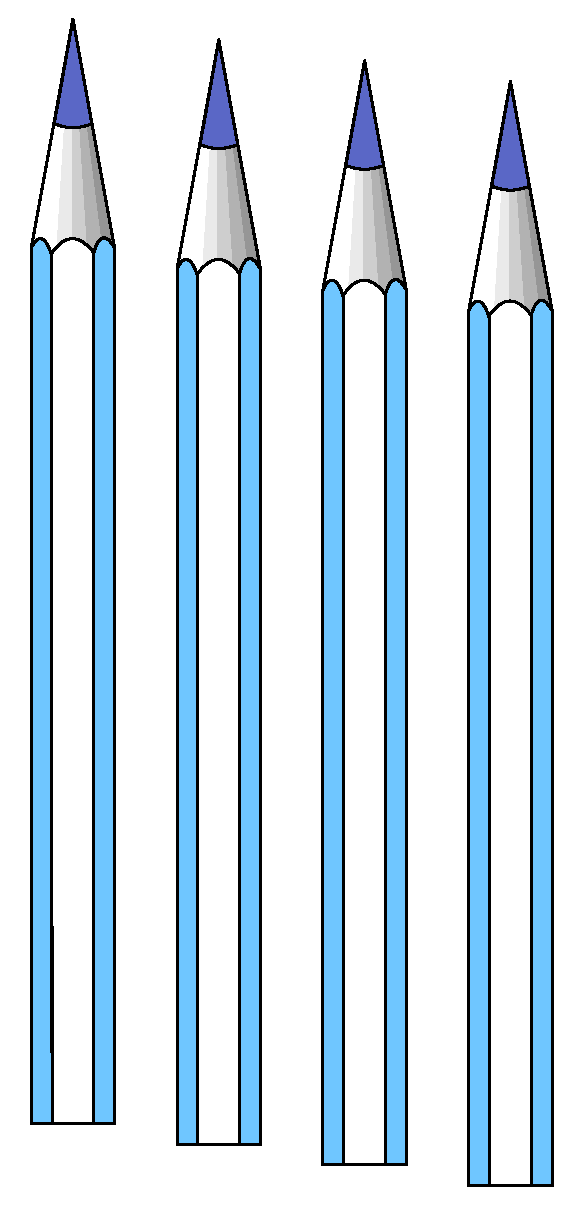
\includegraphics[angle=-90,width=0.9\textwidth]{pencils}}

  \vspace{\stretch{2}}

  %\htmladdnormallink{Wolfgang Dobler}{http://www.kis.uni-freiburg.de/~dobler/}
  %\&
  %\htmladdnormallink{Axel Brandenburg}{http://www.nordita.org/~brandenb/}

  \vspace{\stretch{1}}

  \emph{$ $Date$ $,~ $ $Revision$ $}\\
  \url{http://www.nordita.org/software/pencil-code/}\\
  \url{http://pencil-code.googlecode.com/}

  \vspace{\stretch{3}}

\end{center}

\end{titlepage}


\newpage
\mbox{}

\begin{center}
  {\bf The {\sc Pencil Code}: multi-purpose and multi-user maintained}\\
  \url{http://www.nordita.org/~brandenb/talks/misc/PencilCode04.htm}
\end{center}

% ---------------------------------------------------------------------- %
\begin{figure}[htb]
  \centering
  \includegraphics%
    [width=.99\textwidth,keepaspectratio]%
    {cvsstat}
  \caption{Check-in patterns as a function of time for different
  subroutines. The different users are marked by different symbols
  and different colors.
  }
  \label{cvsstat}
\end{figure}
% ---------------------------------------------------------------------- %

\newpage

\begin{center}
  {\bf Contributors to the code}\\
  (in inverse alphabetical order according to their user name)\\
\end{center}

An up to date list of Pencil Code contributers can be found at
\htmladdnormallink{Google
Code}{https://code.google.com/p/pencil-code/people/list}.

\begin{tabular}{lll}
  wladimir.lyra & \htmladdnormallink{Wladimir Lyra}{http://www.astro.uu.se/~wlyra/} & JPL/Caltech\\
  weezy & \htmladdnormallink{S. Louise Wilkin}{http://www.mas.ncl.ac.uk/~n9405169/} & University of Newcastle\\
  wdobler & \htmladdnormallink{Wolfgang Dobler}{http://www.kis.uni-freiburg.de/~dobler/} & Potsdam\\
  vpariev & \htmladdnormallink{Vladimir Pariev}{http://www.pas.rochester.edu/~vpariev/} & University of Rochester\\
  torkel & \htmladdnormallink{Ulf Torkelsson}{http://fy.chalmers.se/~torkel/} & Chalmers University\\
  %tavo.buk & \htmladdnormallink{Gustavo Guerrero}{http://congformodel.sevensense.co/index.php?option=com_content\&view=article\&id=132&Itemid=173\&lang=es} & Stanford University\\
  tavo.buk & \htmladdnormallink{Gustavo Guerrero}{} & Stanford University\\
  thomas.gastine & \htmladdnormallink{Thomas Gastine}{http://www.mps.mpg.de/homes/gastine/} & MPI for Solar System Research\\
  theine & \htmladdnormallink{Tobias (Tobi) Heinemann}{http://www.damtp.cam.ac.uk/user/theine/} & IAS Princeton \\
  tarek & \htmladdnormallink{Tarek A. Yousef}{http://www.pvv.org/~tarek/} & University of Trondheim\\
  sven.bingert & \htmladdnormallink{Sven Bingert}{http://www.svenbingert.de} & MPI for Solar System Research\\
  steveb & \htmladdnormallink{Steve Berukoff}{http://www.physics.ucla.edu/~steveb/} & UCLA \\
  snod & \htmladdnormallink{Andrew Snodin}{http://www.ncl.ac.uk/math/postgrad/postgrads.htm} & University of Newcastle\\
  pkapyla & \htmladdnormallink{Petri K\"apyl\"a}{http://www.helsinki.fi/~kapyla/} & University of Helsinki\\
  nils.e.haugen & \htmladdnormallink{Nils Erland L.\ Haugen}{http://www.sintef.no/Kontakt-oss/Alle-ansatte/?EmpId=1199} & SINTEF \\
  ngrs & \htmladdnormallink{Graeme R. Sarson}{http://www.mas.ncl.ac.uk/~ngrs/home.html} & University of Newcastle\\
  NBabkovskaia & \htmladdnormallink{Natalia Babkovskaia}{http://www.nordita.org/~nbabkovs/} & University of Helsinki\\
  mreinhardt  & \htmladdnormallink{Matthias Rheinhardt}{http://www.helsinki.fi/~rei/} & University of Helsinki\\
  mkorpi  & \htmladdnormallink{Maarit J.\ Mantere (n\'ee Korpi)}{http://www.helsinki.fi/~mkorpi/} & University of Helsinki\\
  miikkavaisala  & \htmladdnormallink{Miikka V\"ais\"al\"a}{https://tuhat.halvi.helsinki.fi/portal/en/persons/miikka-vaisala(90245497-b541-4d55-8409-03ea3e563d82).html} & University of Helsinki\\
  mee  & \htmladdnormallink{Antony (tOnY) Mee}{http://www.mas.ncl.ac.uk/~n7026413/pencil-code/movies/} & University of Newcastle\\
  mcmillan & \htmladdnormallink{David McMillan}{http://brunhes.eas.yorku.ca/dave/CV/} & York University, Toronto\\
  mattias & \htmladdnormallink{Mattias Christensson}{http://www.nordita.org/~mattias/} & formerly at Nordita\\
  koenkemel  & \htmladdnormallink{Koen Kemel}{http://www.nordita.org/~koen/} & Nordita, Stockholm \\
  karlsson & \htmladdnormallink{Torgny Karlsson}{http://www.nordita.org/people/people.php?variant=single\&cn=Torgny+Karlsson} & Nordita\\
  joishi  & \htmladdnormallink{Jeff S.\ Oishi}{http://cms.jsoishi.org/} & Kavli Institute for Particle Astrophysics \& Cosmology\\
  joern.warnecke  & \htmladdnormallink{J\"orn Warnecke}{http://www.nordita.org/~warnecke/} & Nordita, Stockholm \\
  Iomsn1  & \htmladdnormallink{Simon Candelaresi}{http://www.nordita.org/~iomsn/} & Nordita, Stockholm \\
  fadiesis  & \htmladdnormallink{Fabio Del Sordo}{http://www.nordita.org/~fabio/} & Nordita, Stockholm \\
  dorch & \htmladdnormallink{Bertil Dorch}{http://www.astro.ku.dk/~dorch/} & University of Copenhagen\\
  boris.dintrans & \htmladdnormallink{Boris Dintrans}{http://www.ast.obs-mip.fr/dintrans} &  Observatoire Midi-Pyr\'en\'ees, Toulouse\\
  dhruba.mitra & \htmladdnormallink{Dhrubaditya Mitra}{http://www.nordita.org/~dhruba} &  Nordita, Stockholm\\
  ccyang & \htmladdnormallink{Chia-Chun Yang}{} & Lick Observatory \\
  christer & \htmladdnormallink{Christer Sandin}{http://www.astro.uu.se/~christer/CS_index.html} & University of Uppsala\\
  Bourdin.KIS & \htmladdnormallink{Philippe Bourdin}{http://www.mps.mpg.de/en/projekte/coronal-dynamics/} & MPI for Solar System Research\\
  AxelBrandenburg & \htmladdnormallink{Axel Brandenburg}{http://www.nordita.org/~brandenb/} & Nordita\\
  apichat & \htmladdnormallink{Apichat Neamvonk}{Apichat.Neamvonk@ncl.ac.uk} & University of Newcastle\\
  amjed & \htmladdnormallink{Amjed Mohammed}{http://ehf.uni-oldenburg.de/member.php?nav=staff\&sprache=english\&show=43} & University of Oldenburg\\
  alex.i.hubbard  & \htmladdnormallink{Alex Hubbard}{http://www.linkedin.com/pub/alexander-hubbard/47/906/379} & Am. Museum Nat. History\\
  michiel.lambrechts & \htmladdnormallink{Michiel Lambrechts}{http://pc500.astro.lu.se/~michiel/} & Lund Observatory, Lund University\\
  anders & \htmladdnormallink{Anders Johansen}{http://pc366.astro.lu.se/anders/index_en.php} & Lund Observatory, Lund University
\end{tabular}

\vfill

Copyright \copyright{} 2001--2011 Wolfgang Dobler \& Axel Brandenburg
\bigskip

Permission is granted to make and distribute verbatim copies of
this manual provided the copyright notice and this permission notice
are preserved on all copies.

Permission is granted to copy and distribute modified versions
of this manual under the conditions for verbatim copying,
\index{Manual}
provided that the entire resulting derived work is distributed under the
terms of a permission notice identical to this one.

\clearpage

\begin{center}
  {\bf License agreement and giving credit}\\
\end{center}

The content of all files under
\code{:pserver:\$USER@svn.nordita.org:/var/cvs/brandenb}
are under the GNU General Public License
(\url{http://www.gnu.org/licenses/gpl.html}).

We, the {\sc Pencil Code} community, ask that in publications
and presentations the use of the code (or parts of it)
be acknowledged with reference to the web site
\url{http://www.nordita.org/software/pencil-code/} or (equivalently) to.
\url{http://pencil-code.googlecode.com/}.
As a courtesy to the people involved in developing particularly important
parts of the program (use \cmd{svn annotate src/*.f90} to find out who did what!)
we suggest to give appropriate reference to one or
several of the following (or other appropriate) papers (listed here in temporal order):

\newcommand{\arXiv}[1]{\htmladdnormallink{\sf arXiv/#1}{http://arXiv.org/abs/#1}}
\newcommand{\astroph}[1]{\htmladdnormallink{\sf astro-ph/#1}{http://arXiv.org/abs/astro-ph/#1}}
\newcommand{\condmat}[1]{\htmladdnormallink{\sf cond-mat/#1}{http://arXiv.org/abs/abs/cond-mat/#1}}
\newcommand{\physics}[1]{\htmladdnormallink{\sf physics/#1}{http://arXiv.org/abs/abs/physics/#1}}
\newcommand{\qbio}[1]{\htmladdnormallink{\sf q-bio/#1}{http://arXiv.org/abs/abs/q-bio/#1}}
\newcommand{\yannr}[5]{:~#1, ``#5,'' {\em Ann.\ Rev.\ Astron.\ Astrophys. }{\bf #2}, #3-#4}
\newcommand{\yica}[5]{:~#1, ``#5,'' {\em Icarus }{\bf #2}, #3-#4}
\newcommand{\ysph}[5]{:~#1, ``#5,'' {\em Solar Phys. }{\bf #2}, #3-#4}
\newcommand{\ysphs}[5]{:~#1, ``#5'' {\em Solar Phys. }{\bf #2}, #3-#4}
\newcommand{\ymn}[5]{:~#1, ``#5,'' {\em Monthly Notices Roy. Astron. Soc. }{\bf #2}, #3-#4}
\newcommand{\yan}[5]{:~#1, ``#5,'' {\em Astron. Nachr. }{\bf #2}, #3-#4}
\newcommand{\yana}[5]{:~#1, ``#5,'' {\em Astron. Astrophys. }{\bf #2}, #3-#4}
\newcommand{\yanaN}[4]{:~#1, ``#4,'' {\em Astron. Astrophys. }{\bf #2}, #3}
\newcommand{\yanas}[5]{:~#1, ``#5'' {\em Astron. Astrophys. }{\bf #2}, #3-#4}
\newcommand{\yass}[5]{:~#1, ``#5,'' {\em Astrophys. Spa. Sci. }{\bf #2}, #3-#4}
\newcommand{\yapj}[5]{:~#1, ``#5,'' {\em Astrophys. J. }{\bf #2}, #3-#4}
\newcommand{\yapjl}[5]{:~#1, ``#5,'' {\em Astrophys. J. Lett. }{\bf #2}, #3-#4}
\newcommand{\yapjlS}[5]{:~#1, ``#5'' {\em Astrophys. J. Lett. }{\bf #2}, #3-#4}
\newcommand{\yjfm}[5]{:~#1, ``#5,'' {\em J. Fluid Mech. }{\bf #2}, #3-#4}
\newcommand{\ypepi}[5]{:~#1, ``#5,'' {\em Phys. Earth Planet. Int.}{\bf #2}, #3-#4}
\newcommand{\ygafd}[5]{:~#1, ``#5,'' {\em Geophys. Astrophys. Fluid Dyn. }{\bf #2}, #3-#4}
\newcommand{\sproc}[5]{:~#1, ``#2,'' in {\em #3}, ed.\ #4, #5 (submitted)}
\newcommand{\eproc}[6]{:~#1, ``#2,'' in {\em #3}, \url{#4}, #5}
\newcommand{\pproc}[5]{:~#1, ``#2,'' in {\em #3}, ed.\ #4, #5 (in press)}
\newcommand{\ypr}[5]{:~#1, ``#5,'' {\em Phys. Rev. }{\bf #2}, #3-#4}
\newcommand{\yprN}[5]{:~#1, ``#5,'' {\em Phys. Rev. }{\bf #2}, #3, #4}
\newcommand{\yproc}[7]{:~#1, ``#4,'' in {\em #5}, ed.\ #6, #7, pp.~#2-#3}
\newcommand{\yjourS}[6]{:~#1, ``#6'' {\em #2} {\bf #3}, #4-#5}
\newcommand{\yjour}[6]{:~#1, ``#6,'' {\em #2} {\bf #3}, #4-#5}
\newcommand{\sjour}[3]{:~#1, ``#3,'' {\em #2} (submitted)}
\newcommand{\sjourS}[3]{:~#1, ``#3'' {\em #2} (submitted)}
\newcommand{\pjour}[3]{:~#1, ``#3,'' {\em #2} (in press)}
\newcommand{\pjourS}[3]{:~#1, ``#3'' {\em #2} (in press)}
\newcommand{\ybook}[3]{:~#1,  {\em #2}. #3}
\newcommand{\ypf}[5]{:~#1, ``#5,'' {\em Phys. Fluids }{\bf #2}, #3-#4}
\newcommand{\ypp}[5]{:~#1, ``#5,'' {\em Phys. Plasmas }{\bf #2}, #3-#4}
\newcommand{\yepl}[5]{:~#1, ``#5,'' {\em Europhys. Lett. }{\bf #2}, #3-#4}
\newcommand{\yprl}[5]{:~#1, ``#5,'' {\em Phys. Rev. Lett. }{\bf #2}, #3-#4}
\newcommand{\ybif}[5]{:~#1, ``#5,'' {\em Int. J. Bifurc. Chaos }{\bf #2}, #3-#4}
\newcommand{\ycsf}[5]{:~#1, ``#5,'' {\em Chaos, Solitons \& Fractals }{\bf #2}, #3-#4}
\newcommand{\ycsfS}[5]{:~#1, ``#5'' {\em Chaos, Solitons \& Fractals }{\bf #2}, #3-#4}
\newcommand{\sprl}[2]{:~#1, ``#2,'' {\em Phys. Rev. Lett.} (submitted)}
\newcommand{\pprl}[2]{:~#1, ``#2,'' {\em Phys. Rev. Lett.} (in press)}
\newcommand{\tpr}[3]{:~#1, ``#3,'' {\em Phys. Rev. }{\bf #2} (to be submitted)}
\newcommand{\spr}[3]{:~#1, ``#3,'' {\em Phys. Rev. }{\bf #2} (submitted)}
\newcommand{\ppr}[3]{:~#1, ``#3,'' {\em Phys. Rev. }{\bf #2} (in press)}
\newcommand{\pppp}[3]{:~#1, ``#2,'' {\em Phys. Plasmas} (in press, scheduled for the #3 issue)}
\newcommand{\ppp}[2]{:~#1, ``#2,'' {\em Phys. Plasmas} (in press)}
\newcommand{\spp}[2]{:~#1, ``#2,'' {\em Phys. Plasmas} (submitted)}
\newcommand{\tpp}[2]{:~#1, ``#2,'' {\em Phys. Plasmas} (to be submitted)}
\newcommand{\tppS}[2]{:~#1, ``#2'' {\em Phys. Plasmas} (to be submitted)}
\newcommand{\san}[2]{:~#1, ``#2,'' {\em Astron. Nachr.} (submitted)}
\newcommand{\pan}[2]{:~#1, ``#2,'' {\em Astron. Nachr.} (in press)}
\newcommand{\sana}[2]{:~#1, ``#2,'' {\em Astron. Astrophys.} (submitted)}
\newcommand{\tana}[2]{:~#1, ``#2,'' {\em Astron. Astrophys.} (to be submitted)}
\newcommand{\sanas}[2]{:~#1, ``#2'' {\em Astron. Astrophys.} (submitted)}
\newcommand{\pana}[2]{:~#1, ``#2,'' {\em Astron. Astrophys.} (in press)}
\newcommand{\panas}[2]{:~#1, ``#2'' {\em Astron. Astrophys.} (in press)}
\newcommand{\sgafd}[2]{:~#1, ``#2,'' {\em Geophys. Astrophys. Fluid Dyn.} (submitted)}
\newcommand{\pgafd}[2]{:~#1, ``#2,'' {\em Geophys. Astrophys. Fluid Dyn.} (in press)}
\newcommand{\ppgafd}[3]{:~#1, ``#3,'' {\em Geophys. Astrophys. Fluid Dyn.} {\bf #2}}
\newcommand{\tapj}[2]{:~#1, ``#2,'' {\em Astrophys. J.} (to be submitted)}
\newcommand{\ppapj}[2]{:~#1, ``#2,'' {\em Astrophys. J.} (in press)}
\newcommand{\ppapjl}[2]{:~#1, ``#2,'' {\em Astrophys. J. Lett.} (in press)}
\newcommand{\sapj}[2]{:~#1, ``#2,'' {\em Astrophys. J.} (submitted)}
\newcommand{\sapjS}[2]{:~#1, ``#2'' {\em Astrophys. J.} (submitted)}
\newcommand{\ppapjS}[2]{:~#1, ``#2'' {\em Astrophys. J.} (in press)}
\newcommand{\sapjl}[2]{:~#1, ``#2,'' {\em Astrophys. J. Lett.} (submitted)}
\newcommand{\ppapjlS}[2]{:~#1, ``#2'' {\em Astrophys. J. Lett.} (in press)}
\newcommand{\sapjlS}[2]{:~#1, ``#2'' {\em Astrophys. J. Lett.} (submitted)}
\newcommand{\papj}[4]{:~#1, ``#3,'' {\em Astrophys. J. }{\bf #2} (scheduled for the #4 issue)}
\newcommand{\papjS}[4]{:~#1, ``#3'' {\em Astrophys. J. }{\bf #2} (scheduled for the #4 issue)}
\newcommand{\papjl}[4]{:~#1, ``#3,'' {\em Astrophys. J. Lett. }{\bf #2} (scheduled for the #4 issue)}
\newcommand{\papjlS}[4]{:~#1, ``#3'' {\em Astrophys. J. Lett. }{\bf #2} (scheduled for the #4 issue)}
\newcommand{\ynat}[5]{:~#1, ``#5,'' {\em Nature }{\bf #2}, #3--#4}
\newcommand{\spf}[2]{:~#1, ``#2,'' {\em Phys. Fluids} (submitted)}
\newcommand{\ppf}[2]{:~#1, ``#2,'' {\em Phys. Fluids} (in press)}
\newcommand{\ssph}[2]{:~#1, ``#2,'' {\em Solar Phys.} (submitted)}
\newcommand{\psph}[2]{:~#1, ``#2,'' {\em Solar Phys.} (in press)}
\newcommand{\sbif}[2]{:~#1, ``#2,'' {\em Int. J. Bifurc. Chaos} (submitted)}
\newcommand{\pbif}[2]{:~#1, ``#2,'' {\em Int. J. Bifurc. Chaos} (in press)}
\newcommand{\pjfm}[2]{:~#1, ``#2,'' {\em J. Fluid Mech. } (in press)}
\newcommand{\sjfm}[2]{:~#1, ``#2,'' {\em J. Fluid Mech. } (submitted)}
\newcommand{\tjfm}[2]{:~#1, ``#2,'' {\em J. Fluid Mech. } (to be submitted)}
\newcommand{\pmn}[2]{:~#1, ``#2,'' {\em Monthly Notices Roy. Astron. Soc.} (in press)}
\newcommand{\smn}[2]{:~#1, ``#2,'' {\em Monthly Notices Roy. Astron. Soc.} (submitted)}
\newcommand{\tmn}[2]{:~#1, ``#2,'' {\em Monthly Notices Roy. Astron. Soc.} (to be submitted)}

\begin{list}{}{\leftmargin 3em \itemindent -3em\listparindent \itemindent
\itemsep 0pt \parsep 1pt}\item[]

% -- Isotropic homogeneous hydro turbulence --
Dobler, W., Haugen, N. E. L., Yousef, T. A., \&
Brandenburg, A.\yprN{2003}{E 68}{026304}
{1-8}{Bottleneck effect in three-dimensional turbulence simulations}
(\astroph{0303324})

% -- Isotropic homogeneous MHD turbulence --
Haugen, N. E. L., Brandenburg, A., \& Dobler, W.\yapjlS{2003}{597}{L141}
{L144}{Is nonhelical hydromagnetic turbulence peaked at small scales?}
(\astroph{0303372})

% -- Passive scalar diffusion --
Brandenburg, A., K\"apyl\"a, P., \& Mohammed, A.\ypf{2004}{16}{1020}
{1027}{Non-Fickian diffusion and tau-approximation from numerical turbulence}
(\astroph{0306521})

% -- Dust in the fluid approximation --
Johansen, A., Andersen, A. C., \& Brandenburg, A.\yana{2004}{417}{361}
{371}{Simulations of dust-trapping vortices in protoplanetary discs}
(\astroph{0310059})

% -- Supersonic turbulence --
Haugen, N. E. L., Brandenburg, A., \& Mee, A. J.\ymn{2004}{353}{947}
{952}{Mach number dependence of the onset of dynamo action}
(\astroph{0405453})

% -- Homochirality --
Brandenburg, A., \& Multam\"aki, T.\yjourS{2004}{Int.\ J.\ Astrobiol.}{3}{209}
{219}{How long can left and right handed life forms coexist?}
(\qbio{0407008})

% -- Geodynamo --
McMillan, D. G., \& Sarson, G. R.\ypepi{2005}{153}{124}
{135}{Dynamo simulations in a spherical shell of ideal gas using a
high-order Cartesian magnetohydrodynamics code}

% -- Radiation transfer --
Heinemann, T., Dobler, W., Nordlund, \AA., \&
Brandenburg, A.\yana{2006}{448}{731}
{737}{Radiative transfer in decomposed domains}
(\astroph{0503510})

% -- Star-in-a-box simulation --
Dobler, W., Stix, M., \& Brandenburg, A.\yapj{2006}{638}{336}
{347}{Convection and magnetic field generation in fully convective spheres}
(\astroph{0410645})

% -- Cosmic ray diffusion --
Snodin, A. P., Brandenburg, A., Mee, A. J., \& Shukurov, A.\ymn{2006}{373}{643}
{652}{Simulating field-aligned diffusion of a cosmic ray gas}
(\astroph{0507176})

% -- Dust represented as particles --
Johansen, A., Klahr, H., \& Henning, T.\yapj{2006}{636}{1121}
{1134}{Dust sedimentation and self-sustained Kelvin-Helmholtz turbulence
in protoplanetary disc mid-planes}
(\astroph{0512272})

% -- Core accretion in the context of Code comparison --
de Val-Borro, M. and 22 coauthors (incl.\ Lyra, W.)\ymn{2006}{370}{529}
{558}{A comparative study of disc-planet interaction}
(\astroph{0605237})

% -- Self-gravity --
Johansen, A., Oishi, J. S., Mac Low, M. M., Klahr, H., Henning, T.,
\& Youdin, A.\ynat{2007}{448}{1022}
{1025}{Rapid planetesimal formation in turbulent circumstellar disks}
(\arXiv{0708.3890})

% -- Global models of protoplanetary disks --
Lyra, W., Johansen, A., Klahr, H., \& Piskunov, N.\yana{2008}{479}{883}
{901}{Global magnetohydrodynamical models of turbulence in protoplanetary disks I. A cylindrical potential on a Cartesian grid and transport of solids}
(\arXiv{0705.4090})

% -- Test-field method --
Brandenburg, A., R\"adler, K.-H., Rheinhardt, M., \& K\"apyl\"a, P. J.\yapj{2008}{676}{740}
{751}{Magnetic diffusivity tensor and dynamo effects in rotating
and shearing turbulence}
(\arXiv{0710.4059})

% -- Global simulations of planet formation --
Lyra, W., Johansen, A., Klahr, H., \& Piskunov, N.\yana{2008}{491}{L41}{L44}{Embryos grown in the dead zone. Assembling the first protoplanetary cores in low-mass selfgravitating circumstellar disks of gas and solids}

% -- N-body solver --
Lyra, W., Johansen, A., Klahr, H., \& Piskunov, N.\yana{2009}{493}{1125}
{1139}{Standing on the shoulders of giants. Trojan Earths and vortex trapping in low-mass selfgravitating protoplanetary disks of gas and solids}

% -- Cylindrical grid --
Lyra, W., Johansen, A., Zsom, A., Klahr, H., \& Piskunov, N.\yana{2009}{497}{869}
{888}{Planet formation bursts at the borders of the dead zone in 2D numerical simulations of circumstellar disks}
(\arXiv{0901.1638})

% -- Spherical coordinates --
Mitra, D., Tavakol, R., Brandenburg, A., \& Moss, D.\yapj{2009}{697}{923}
{933}{Turbulent dynamos in spherical shell segments of varying geometrical extent} (\arXiv{0812.3106})

% -- Particle impaction on a cylinder --
Haugen, N. E. L., \& Kragset, S.\yjfm{2010}{661}{239}
{261}{Particle impaction on a cylinder in a crossflow as function of Stokes and Reynolds numbers}

% -- Nonlinear test-field method --
Rheinhardt, M., \& Brandenburg, A.\yanaN{2010}{520}{A28}
{Test-field method for mean-field coefficients with MHD background}
(\arXiv{1004.0689})

% -- Turbulent combustion --
Babkovskaia, N., Haugen, N. E. L., Brandenburg, A.\yjour{2011}{J.\ Comp.\ Phys.}{230}{1}
{12}{A high-order public domain code for direct numerical simulations of turbulent combustion}
(\arXiv{1005.5301})

% -- superparticles --
Johansen, A., Youdin, A. N., \& Lithwick, Y.\yanaN{2012}{537}{A125}
{Adding particle collisions to the formation of asteroids and Kuiper belt objects via streaming instabilities}

\end{list}
This list is not always up-to-date.
We therefore ask the developers to check in new relevant papers,
avoiding however redundancies.
\clearpage

% ====================================================================== %

\section*{Foreword}

This code was originally developed at the Turbulence Summer School of the
Helmholtz Institute in Potsdam (2001).
While some SPH and PPM codes for hydrodynamics and magnetohydrodynamics
are publicly available, this does not generally seem to be
the case for higher order finite-difference or spectral codes.
Having been approached by people interested in using our code, we
decided to make it as flexible as possible and as user-friendly as seems
reasonable, and to put it onto a public \name{CVS} repository.
Since 21 September 2008 it is distributed via
\url{http://code.google.com/p/pencil-code/}.
The code can certainly not be treated as a black box (no code can), and in
order to solve a new problem in an optimal way, users will need to find their
own optimal set of parameters.
In particular, you need to be careful in choosing
the right values of viscosity, magnetic diffusivity, and radiative
conductivity.

The {\sc Pencil Code} is primarily designed to deal with weakly compressible
turbulent flows, which is why we use high-order first and second derivatives.
To achieve good parallelization, we use explicit
(as opposed to compact) finite differences.
Typical scientific targets include driven MHD turbulence in a periodic box,
convection in a slab with non-periodic upper and lower boundaries,
a convective star embedded in a fully nonperiodic box, accretion disc
turbulence in the shearing sheet approximation, etc.
Furthermore, nonlocal radiation transport, inertial particles,
dust coagulation, self-gravity, chemical reaction networks, and several
other physical components are installed, but this number increases steadily.
In addition to Cartesian coordinates, the code can also deal with spherical
and cylindrical polar coordinates.

Magnetic fields are implemented in terms of the magnetic vector potential
to ensure that the field remains solenoidal (divergence-free).
At the same time, having the magnetic
vector potential readily available is a big advantage if
one wants to monitor the magnetic helicity, for example.
The code is therefore particularly well suited for all kinds of
dynamo problems.

The code is normally non-conservative; thus, conserved quantities should only be
conserved up to the discretization error of the scheme (not to machine
accuracy).
There is no guarantee that a conservative code is more accurate with
respect to quantities that are not explicitly conserved, such as entropy.
Another important quantity that is (to our knowledge) not strictly
conserved by ordinary flux conserving schemes is \name{magnetic helicity}.

There are currently no plans to implement adaptive mesh refinement
into the code, which would cause major technical complications.
Given that turbulence is generically space-filling, local refinement
to smaller scales would often not be very useful anyway.
On the other hand, in some geometries
turbulence may well be confined to certain regions in space, so one
could indeed gain by solving the outer regions with fewer points.

In order to be cache-efficient, we solve the equations along
\name{pencils} in the $x$ direction.
One very convenient side-effect is that auxiliary and derived variables
use very little memory, as they are only ever defined on one pencil.
The domain can be tiled in the $y$ and $z$ directions.
On multiprocessor computers, the code can use \name{MPI}
(Message Passing Interface) calls to communicate between processors.
An easy switching mechanism allows the user to run the code on a machine
without MPI libraries (e.g.\ a notebook computer).
Ghost zones are used to implement boundary conditions on physical and
processor boundaries.

A high level of flexibility is achieved by encapsulating individual
physical processes and variables in individual \name{modules}, which can
be switched on or off in the file \file{Makefile.local} in the local
\file[src/]{src} directory.
This approach avoids the use of difficult-to-read preprocessor directives,
at the price of requiring one dummy module for each physics module.
For nonmagnetic hydrodynamics, for example, one will use the module
\file{nomagnetic.f90} and specifies
\begin{Verbatim}
  MAGNETIC=nomagnetic
\end{Verbatim}
in \file{Makefile.local},
while for MHD simulations, \file{magnetic.f90} will be used:
\begin{Verbatim}
  MAGNETIC=magnetic
\end{Verbatim}
Note that the term \name{module} as used here is only loosely related to
Fortran modules:
both \file{magnetic.f90} and \file{nomagnetic.f90} define an F90
module named \emph{Magnetic} --- this is the basis of the switching
mechanism we are using.

Input parameters (which are set in the files \file{start.in},
\file{run.in}) can be changed without recompilation.
Furthermore, one can change the list of variables for monitoring
(diagnostic) output on the fly, and there are mechanisms for making the
code reload new parameters or exit gracefully at runtime.

The requirements for using the Pencil-MPI code are modest: you can use it
on any Linux or Unix system with a F90/F95 compiler.
Although the {\sc Pencil Code} is mainly designed to run on supercomputers,
more than 50\% of the users run their code also on Macs, and the other half
uses either directly Linux on their laptops or they use VirtualBox
on their Windows machine on which they install Ubuntu Linux.
If you have \name{IDL} as
well, you will be able to visualize the results (a number of sample
procedures are provided), but other tools such as
\name{Python}, \name{DX} (OpenDX, data explorer) can also be used
and some relevant tools and routines come with the {\sc Pencil Code}.

\bigskip

If you want to make creative use of the code, this manual will contain far
too little information.
Its major aim is to give you an idea of the way the code is organized, so
you can more efficiently \emph{read the source code}, which contains a
reasonable amount of comments.
You might want to read through the various sample directories that are checked in.
Choose one that is closest to your application and start modifying.
For further enhancements that you may want to add to the code, you can
take as an example the lines in the code that deal with related variables,
functions, diagnostics, equations etc., which have already been implemented.
Just remember: \cmd{grep} is one of your best friends when you want to
understand how certain variables or functions are used in the code.

\bigskip

We will be happy to include user-supplied changes and updates to the code
in future releases and welcome any feedback.

\vspace{5mm}
%\noindent
%\email{Wolfgang.Dobler@kis.uni-freiburg.de}\hfill Freiburg\\
\email{wdobler@gmail.com}\hfill Potsdam\\
\email{AxelBrandenburg@gmail.com}\hfill Stockholm
%Wolfgang's new company: www.jpk.com

% ====================================================================== %

\section*{Acknowledgments}

Many people have contributed in different ways to the development of this
code. We thank first of all {\AA}ke Nordlund (Copenhagen Observatory)
and Bob Stein (University of Michigan) who introduced us to the idea of
using high-order schemes in compressible flows and who taught us a lot
about simulations in general.

The calculation of the power spectra, structure functions,
the remeshing procedures,
routines for changing the number of processors, as well as
the shearing sheet approximation and the flux-limited diffusion
approximation for radiative transfer
were implemented by Nils Erland L.\ Haugen (University of Trondheim).
Tobi Heinemann added the long characteristics method for
radiative transfer as well as hydrogen ionization.
He also added and/or improved shock diffusion for other variables
and improved the resulting timestep control.
Anders Johansen, Wladimir (Wlad) Lyra, and Jeff Oishi contributed
to the implementation of
the dust equations (which now comprises an array of different components).
Antony (Tony) Mee (University of Newcastle) implemented shock viscosity
and added the interstellar module together with
Graeme R.\ Sarson (also University of Newcastle), who also implemented
the geodynamo set-up together with David McMillan
(currently also at the University of Newcastle).
Tony also included a method for outputting auxiliary variables and
enhanced the overall functionality of the code and related idl and dx
procedures.
He also added, together with Andrew Snodin, the evolution equations
for the cosmic ray energy density.
Vladimir Pariev (University of Rochester) contributed to the development
and testing of the potential field boundary condition at an early stage.
The implementation of spherical and cylindrical coordinates is due
to Dhrubaditya (Dhruba) Mitra and Wladimir Lyra. Wlad also
implemented the global set-up for protoplanetary
disks (as opposed to the local shearing sheet formalism). He also added a
$N$-body code (based on the particle module coded by Anders Johansen
and Tony), and implemented the coupled evolution equations of neutrals and
ions for two-fluid models of ambipolar diffusion.
Boris Dintrans is in charge of implementing the anelastic and Boussinesq modules.
Philippe-A. Bourdin implemented HDF5 support and wrote the optional IO-modules
for high-performance computing featuring various communication strategies.
He also contributed to the solar-corona module and worked on the IDL GUI,
including the IDL routines for reading and working with large amounts of data.
Again, this list contains other recent items that are not yet fully
documented and acknowledged.

Use of the PPARC supported supercomputers in St Andrews (Mhd) and
Leicester (Ukaff) is acknowledged. We also acknowledge the Danish Center
for Scientific Computing for granting time on Horseshoe, which is a
512+140 processor Beowulf cluster in Odense (Horseshoe).

\clearpage
\tableofcontents
\cleardoublepage
\pagestyle{fancy}
\pagenumbering{arabic}


% ====================================================================== %

\part{Using the {\sc Pencil Code}}

\section{System requirements}

To use the code, you will need the following:

\begin{enumerate}

\item Absolutely needed:
  \begin{itemize}
  \item \name{F95} compiler
  \item \name{C} compiler
  \end{itemize}

\item Used heavily (if you don't have one of these, you will need to
  adjust many things manually):
  \begin{itemize}
  \item a \name{Unix}/\name{Linux}-type system with \name{make} and \name{csh}
  \item \name{Perl} (remember: if it doesn't run Perl, it's not a
    computer)
  \end{itemize}

\item The following are dispensable, but enhance functionality in one
  way or the other:
  \begin{itemize}
  \item an \name{MPI} implementation (for parallelization on
    multiprocessor systems)
  \item \name{DX} alias \name{OpenDX} or \name{data explorer} (for
    3-D visualization of results)
  \item \name{IDL} (for visualization of results; the 7-minute demo
    license will do for many applications)
  \end{itemize}

\end{enumerate}

%If you like the exotic and get the code running in a \name{Cygwin}
%environment, please let us know.


% ====================================================================== %

\section{Obtaining the code}
\index{Download}
\label{Download}

The code is now distributed via
\url{http://code.google.com/p/pencil-code/},
where you can either download a tarball, or, preferably,
download it via \name{svn}.
In Iran and some other countries, Google Code is not currently available.
To alleviate this problem, we have made a recent copy available on
\url{http://www.nordita.org/software/pencil-code/}.
If you want us to update this tarball, please contact us.

To ensure at least some level of stability of the \name{svn}
versions, a set of test problems (listed in
\file[auto-test]{\$PENCIL_HOME/bin/auto-test})
are routinely tested.
This includes all problems in
\file[samples/]{\$PENCIL_HOME/samples}.
See Sect.~\ref{S-Testing} for details.

% ---------------------------------------------------------------------- %

\subsection{Obtaining the code via svn}
\index{CVS}
\index{svn}

\begin{enumerate}

\item Many machines have \name{svn} installed
  (try \code{svn -v} or \code{which svn}).
  On Ubuntu, for example, \name{svn} comes under the
  package name subversion.

\item Unless you are a privileged users with write access, you can
  download the code with the command
  \begin{verbatim}
    svn checkout http://pencil-code.googlecode.com/svn/trunk/ pencil-code
  \end{verbatim}
  Privileged users with write access to the original repository should use
  something like
  \begin{verbatim}
    svn checkout https://pencil-code.googlecode.com/svn/trunk/ pencil-code --username USERNAME
  \end{verbatim}
  where \name{USERNAME} is to be replaced by {\it your} googlecode user name.
  Note that the svn password is not the usual google password, but it is the
  more complicated character string generated by google when clicking on
  $\to$ profile $\to$ settings.
  There it says ``Your googlecode.com password: ...''.

  Be sure to run \code{auto-test} before you check anything back in again.
  It can be very annoying for someone else to figure out what's wrong,
  especially if you are just up to something else.
  At the very least, you should do
  \begin{verbatim}
    pc_auto-test --level=0 --no-pencil-check -C
  \end{verbatim}
  This allows you to run just 2 of the most essential tests starting
  with all the no-modules and then most-modules.

\end{enumerate}

% ---------------------------------------------------------------------- %

\subsection{Updating via svn}
\index{svn}

Independent of how you installed the code in the first place (from tarball
or via \name{svn}), you can update your version using \name{svn}.
If you have done nontrivial alterations to your version of the code, you
ought to be careful about upgrading: although \name{svn} is an excellent
tool for distributed programming,
conflicts are quite possible, since many of us are going to
touch many parts of the code while we develop it further.
Thus, despite the fact that the code is under \name{svn}, you should probably
back up your important changes before upgrading.

Here is the upgrading procedure:
\begin{enumerate}
\item Perform a \cmd{svn} update of the tree:
  \begin{alltt}
  \prompt{unix> } pc_svnup \
  \end{alltt}
\item Fix any conflicts you encounter and make sure the examples in the
  directory \file{samples/} are still working.
\end{enumerate}

If you have made useful changes, please contact one of the (currently) 10
``Owners'' (listed under \url{https://code.google.com/p/pencil-code/people/list})
who can give you check-in permission.
Be sure to have sufficient comments in the code and please follow our
standard coding conventions explained in Section~\ref{ProgrammingStyle}.

% ---------------------------------------------------------------------- %

\subsection{Getting the last validated version}
\index{svn}

The script \cmd{pc_svnup} accepts arguments -val or -validated, which
means that the current changes on a user's machine will be merged
into the last working version. This way every user can be sure that
any problems with the code must be due to the current changes done
by this user since the last check-in.

Examples:
  \begin{alltt}
  \prompt{unix> } pc_svnup -src -s -validated\
  \end{alltt}

brings all files in \file[src/]{\$PENCIL_HOME/src} to the last validated
status, and merges all your changes into this version. This allows you
to work with this, but in order to check in your changes you have to
update everything to the most recent status first, i.e.
  \begin{alltt}
  \prompt{unix> } pc_svnup -src\
  \end{alltt}
Your own changes will be merged into this latest version as before.

NOTE: The functionality of the head of the trunk should be preserved
at all times. However, accidents do happen. For the benefit of all
other developers, any errors should be corrected within 1-2 hours.
This is the reason why the code comes with a file
\file{pencil-code/license/developers.txt},
which should contain contact details of all developers.
The \cmd{pc_svnup -val} option allows all other people to stay away
from any trouble.

% ---------------------------------------------------------------------- %

\subsection{Getting older versions}
\index{svn}

You may find that the latest \name{svn} version of the code produces errors.
If you have reasons to believe that this is due to changes introduced on
27 November 2008 (to give an example), you can check out the version prior to
this by specifying a revision number with \cmd{svn update -r \#\#\#\#\#}.
One reason why one cannot always reproduce exactly the same situation too far
back in time is connected with the fact that processor architecture and the
compiler were different, resulting e.g. in different rounding errors.

% ---------------------------------------------------------------------- %

%\subsection{Obtaining and unpacking the tarball}
%
%\begin{enumerate}
%\item Download the tarball file, pencil-code_X.tar.gz,
%  where X is the release number, after registering on
%  \url{http://www.nordita.org/software/pencil-code/}
%\item Put it into a convenient directory and unpack it:
%  \begin{alltt}
%  \prompt{unix> } mv pencil-code_X.tar.gz somewhere/; cd somewhere
%  \prompt{unix> } gunzip pencil-code_X.tar.gz
%  \prompt{unix> } tar xf pencil-code_X.tar \
%  \end{alltt}
%\end{enumerate}


% ====================================================================== %

\section{Getting started}
\label{S-getting-started}

To get yourself started, you should run one or several examples which are
provided in one of the \file{samples/} subdirectories.
Note that you will only be able to fully assess the numerical solutions if you
visualize them with \name{IDL}, \name{DX} or other tools (see
Sect.~\ref{S-Visualization}).

% ---------------------------------------------------------------------- %

\subsection{Setup}
\index{Setup}

\subsubsection{Environment settings}

The functionality of helper scripts and IDL routines relies on a few
environment variables being set correctly.
The simplest way to achieve this is to go to the top directory of the code
and source one of
the two scripts \file{sourceme.csh} or \file{sourceme.sh} (depending on
the type of shell you are using):
\begin{alltt}
  \prompt{csh> } cd pencil-code
  \prompt{csh> } source ./sourceme.csh
\end{alltt}
for \name{tcsh} or \name{csh} users; or
\begin{alltt}
  \prompt{sh> } cd pencil-code
  \prompt{sh> } . ./sourceme.sh
\end{alltt}
for users of \name{bash}, \name{Bourne shell}, or similar shells.
You should get output similar to
\begin{alltt}
  PENCIL_HOME = </home/dobler/f90/pencil-code>
  Adding /home/dobler/f90/pencil-code/bin to PATH
\end{alltt}
Apart from the \env{PATH} variable, the environment variable
\env{IDL_PATH} is set to something like
\texttt{./idl:../idl:+\$PENCIL_HOME/idl:./data:<IDL_DEFAULT>} .

\paragraph{Note 1}
The \code{<IDL_DEFAULT>} mechanism does not work for IDL versions 5.2 or
older. In this case, you will have to edit the path manually, or adapt
the \file{sourceme} scripts.

\paragraph{Note 2}
If you  don't want to rely on the \file{sourceme} scripts' (quite
heuristic) ability to correctly identify the code's main directory, you
can set the environment variable
\env{PENCIL_HOME} explicitly before you run the source command.

\paragraph{Note 3}
Do not just source the \file{sourceme} script from your shell startup file
(\file[.cshrc]{\~{}/.cshrc} or \file[.bashrc]{\~{}/.bashrc}, because it
outputs a few lines of diagnostics for each sub-shell, which will break
many applications.
To suppress all output, follow the instructions given in the header
documentation of \file{sourceme.csh} and \file{sourceme.sh}.

\paragraph{Note 4}
The second time you source \file{sourceme}, it will not add
anything to your \env{PATH} variable.
This is on purpose to avoid cluttering of your environment: you can
source the file as often as you like (in your shell startup script, then
manually and in addition in some script you have written), without
thinking twice.
If, however, at the first sourcing, the setting of \env{PENCIL_HOME} was
wrong, this mechanism would keep you from ever adding the right directory
to your \env{PATH}.
In this case, you need to first undefine the environment variable
\env{PENCIL_HOME}:
\begin{alltt}
  \prompt{csh> } unsetenv PENCIL_HOME
  \prompt{csh> } source ./sourceme.csh
  {\sl{}or}
  \prompt{sh> } unset PENCIL_HOME
  \prompt{sh> } . ./sourceme.sh
\end{alltt}



\subsubsection{Linking scripts and source files}

With your environment set up correctly, you can now go to the directory
you want to work in and set up subdirectories and links.
This is accomplished by the script \file{pc_setupsrc}, which is located in
\file[bin/]{\$PENCIL_HOME/bin} and is thus now in your executable path.

For concreteness, let us assume you want to use
\file[conv-slab/]{samples/conv-slab}
as your \dfn{run directory}, i.e.\ you want to run a three-layer slab model
of solar convection.
You then do the following:
\begin{alltt}
  \prompt{unix> } cd samples/conv-slab
  \prompt{unix> } pc_setupsrc
  src already exists
  2 files already exist in src
\end{alltt}
The script has linked a number of scripts from \file[bin/]{\$PENCIL_HOME/bin},
generated a directory \file[src/]{src} for the source code and linked the
Fortran source files (plus a few more files) from \file[src/]{\$PENCIL_HOME/src}
to that directory:
\begin{alltt}
  \prompt{unix> } ls -F
  reference.out  src/
  start.csh@     run.csh@  getconf.csh@
  start.in       run.in    print.in
\end{alltt}


\subsubsection{Adapting \file{Makefile.src}}
\index{Makefile}

This step requires some input from you, but you only have to do this once
for each machine you want to run the code on.
See Sect.~\ref{adapt-mkfile} for a description of the steps you need to
take here.

\paragraph{Note:} If you are lucky and use compilers similar to the ones
we have, you may be able to skip this step; but blame yourself if things
don't compile, then.
If not, you can run \cmd{make} with explicit flags, see
Sect.~\ref{S-make-flags} and in particular Table~\ref{Tab-compiler-options}.


\subsubsection{Running \cmd{make}}

Next, you run \cmd{make} in the \file[src/]{src} subdirectory of your run
directory.
Since you are using one of the predefined test problems, the settings in
\file[Makefile.local]{src/Makefile.local} and
\file[cparam.local]{src/cparam.local} are all reasonable, and you just do
\begin{alltt}
  \prompt{unix> } make \
\end{alltt}
If you have set up the compiler flags correctly, compilation should
complete successfully.


\subsubsection{Choosing a data directory}

The code will by default write data like snapshot files to the subdirectory
\file[data/]{data} of the run directory.
Since this will involve a large volume of IO-operations (at least for
large grid sizes), one will normally try to avoid writing the data via
NFS.
The recommended way to set up a \file[data/]{data} data directory is to generate
a corresponding directory on the local disc of the computer you are
running on and (soft-)link it to \file[data/]{./data}.
Even if the link is part of an NFS directory, all the IO operations will
be local.
For example, if you have a local disc \file[/scratch/]{/scratch}, you can
do the following:
\begin{alltt}
  \prompt{unix> } mkdir -p /scratch/\$USER/pencil-data/samples/conv-slab
  \prompt{unix> } ln -s /scratch/\$USER/pencil-data/samples/conv-slab ./data \
\end{alltt}
This is done automatically by the \cmd{pc_mkdatadir}
command which, in turn, is invoked when making a new run directory with
the \cmd{pc_newrun} command, for example.

Even if you don't have an NFS-mounted directory (say, on your notebook
computer), it is probably still a good idea to have code and data well
separated by a scheme like the one described above.

An alternative to symbolic links, is to provide a file called
\file{datadir.in} in the root of the run directory.  This file
should contain one line of text specifying the absolute or relative data
directory path to use.  This facility is useful if one wishes to switch
one run directory between different data directories.  It is suggested
that in such cases symbolic links are again made in the run directory
to the various locations, then the \file{datadir.in} need
contain only a short relative path.

\subsubsection{Running the code}

You are now ready to start the code:
\begin{alltt}
  \prompt{unix> } start.csh\small
  Linux cincinnatus 2.4.18-4GB #1 Wed Mar 27 13:57:05 UTC 2002 i686 unknown
  Non-MPI version
  datadir = data
  Fri Aug  8 21:36:43 CEST 2003
     src/start.x
  CVS: io_dist.f90        v. 1.61         (brandenb  ) 2003/08/03 09:26:55
  {\sl{}[\ldots]}
  CVS: start.in           v. 1.4          (dobler    ) 2002/10/02 20:11:14
   nxgrid,nygrid,nzgrid=          32          32          32
   thermodynamics: assume cp=1

   uu: up-down
   piecewise polytropic vertical stratification (lnrho)
   init_lnrho: cs2bot,cs2top=   1.450000      0.3333330
   e.g. for ionization runs: cs2bot,cs2top not yet set
   piecewise polytropic vertical stratification (ss)

   start.x has completed successfully

  0.070u 0.020s 0:00.14 64.2%     0+0k 0+0io 180pf+0w

  Fri Aug  8 21:36:43 CEST 2003
\end{alltt}
This runs \file[start.x]{src/start.x} to construct an initial condition based on
the parameters set in \file{start.in}.
This initial condition is stored in \file[var.dat]{data/proc0/var.dat} (and
in \file[var.dat]{data/proc1/var.dat}, etc.\ if you run the multiprocessor
version).
It is fair to say that this is now a rather primitive routine; see
\file{pencil-code/idl/read} for various reading routines.
You can then visualize the data using standard idl language.

If you visualize the profiles using \name{IDL} (see below),
the result should bear some resemblance to Fig.~\ref{Fig-pvert1}, but with
different values in the ghost zones (the correct values are set at
run-time only) and a simpler velocity profile.

\bigskip

Now we run the code:
\begin{alltt}
  \prompt{unix> } run.csh
\end{alltt}
This runs \file[run.x]{src/run.x} and carries out \var{nt} time steps, where
\var{nt} and other run time parameters are specified in \file{run.in}.
On a decent PC (1.7\,GHz), 50 time steps take about 10 seconds.

The relevant part of the code's output looks like\\
\begin{minipage}{1\textwidth}
\bigskip
\begin{small}
\begin{alltt}
 --it----t-------dt-------urms----umax----rhom------ssm-----dtc----dtu---dtnu---dtchi-
    0   0.34  6.792E-03  0.0060  0.0452  14.4708  -0.4478  0.978  0.013  0.207  0.346
   10   0.41  6.787E-03  0.0062  0.0440  14.4707  -0.4480  0.978  0.013  0.207  0.345
   20   0.48  6.781E-03  0.0064  0.0429  14.4705  -0.4481  0.977  0.012  0.207  0.345
   30   0.54  6.777E-03  0.0067  0.0408  14.4703  -0.4482  0.977  0.012  0.207  0.345
   40   0.61  6.776E-03  0.0069  0.0381  14.4702  -0.4482  0.977  0.011  0.207  0.346
\end{alltt}
\end{small}
\bigskip
\end{minipage}
and lists
\begin{enumerate}
\item the number \var{it} of the current time step;
\item the time, \var{t};
\item the time step, \var{dt};
\item the rms velocity, \var{urms}$\,=\sqrt{\left<\uv^2\right>}$;
\item the maximum velocity, \var{umax}$\,=\max |\uv|$;
\item the mean density, \var{rhom}$\,=\left<\rho\right>$;
\item the mean entropy, \var{ssm}$\,=\left<s\right>/c_p$;
\item the time step in units of the acoustic Courant step,
  \var{dtc}$\,=\delta t/({\cs}_0\,\delta x_{\rm min})$;
\item the time step in units of the advective time step,
  \var{dtu}$\,=\delta t/(c_{\delta t}\,\delta x/\max|\mathbf{u}|)$;
\item the time step in units of viscous time step,
  \var{dtnu}$\,=\delta t/(c_{\delta t,{\rm v}}\,\delta x^2/\nu_{\rm max})$;
\item the time step in units of the conductive time step,
  \var{dtchi}$\,=\delta t / (c_{\delta t,{\rm v}}\,\delta x^2/\chi_{\rm max})$.
\end{enumerate}
The entries in this list can be added, removed or reformatted in the file
\file{print.in}, see Sects~\ref{diagnostic-IO} and \ref{S-print.in-params}.
The output is also saved in \file[time_series.dat]{data/time_series.dat}
and should be identical to the content of \file{reference.out}.

% ---------------------------------------------------------------------- %
\begin{figure}[hbtp]
  \centering
  \includegraphics%
    [width=1\textwidth,keepaspectratio]%
    {pvert1}
  \caption{Stratification of the three-layer convection model in
    \file[conv-slab/]{samples/conv-slab} after $50$ timesteps ($t=0.428$).
    Shown are (from left to right) density $\rho$, vertical velocity
    $u_z$, entropy $s/c_p$ and temperature $T$ as functions of the
    vertical coordinate $z$ for about ten different vertical lines in the
    computational box.
    The dashed lines denote domain boundaries:
    $z<-0.68$ is the lower ghost zone (points have no physical significance);
    $-0.68<z<0$ is a stably stratified layer ($ds/dz>0$);
    $0<z<1$ is the unstable layer ($ds/dz<0$);
    $1<z<1.32$ is the isothermal top layer;
    $z>1.32$ is the upper ghost zone (points have no physical significance).
  }
  \label{Fig-pvert1}
\end{figure}
% ---------------------------------------------------------------------- %

If you have \name{IDL}, you can visualize the stratification with (see
Sect.~\ref{S-IDL-routines} for details)
\begin{alltt}
  \prompt{unix > } idl
  \prompt{IDL >  } .r start
  \prompt{IDL >  } .r r
  \prompt{IDL >  } .r thermo
  \prompt{IDL >  } .r pvert \
\end{alltt}
The result should look like Fig.~\ref{Fig-pvert1}.


\paragraph{Note:}
If you want to run the code with \name{MPI}, you will probably need to
adapt \file{getconf.csh}, which defines the commands and flags used to
run MPI jobs (and which is sourced by the scripts \file{start.csh} and
\file{run.csh}).
Try
\begin{alltt}
  csh -v getconf.csh
  {\sl or}
  csh -x getconf.csh
\end{alltt}
to see how \file{getconf.csh} makes its decisions. You would add a
section for the host name of your machine with the particular settings.
Since \file{getconf.csh} is linked from the central directory
\file[bin/]{pencil-code/bin}, your changes will be
useful for all your other runs too.

% ---------------------------------------------------------------------- %

\subsection{Further tests}

There is a number of other tests in the \file{samples/} directory.
You can use the script \file[auto-test]{bin/auto-test} to automatically run
these tests and have the output compared to reference results.

% ====================================================================== %

\section{Code structure}

\subsection{Directory tree}

 % ---------------------------------------------------------------------- %
\begin{figure}[hbtp]
  \centering
  \includegraphics%
    [width=0.9\textwidth,height=0.65\textheight,keepaspectratio]%
    {struct}
  \caption{The basic structure of the code}
  \label{Fig-Structure}
\end{figure}
% ---------------------------------------------------------------------- %

The overall directory structure of the code is shown in
Fig.~\ref{Fig-Structure}.
Under \file[pencil-code/]{pencil-code}, there are currently the following
files and directories:
\begin{verbatim}
bin/   config/  doc/  idl/  license/  perl/   samples/      sourceme.sh  utils/
bugs/  dx/   lib/  misc/     README  sourceme.csh  src/         www/
\end{verbatim}

Almost all of the source code is contained in the directory \file{src/},
but in order to encapsulate individual applications, the code is compiled
separately for each run in a local directory \file[src/]{src} below the
individual run directory, like
e.\,g.~\file[conv-slab/src/]{samples/conv-slab/src}.

It may be a good idea to keep your own runs also under \name{svn} or
\name{cvs} (which is older than but similar to \name{svn}), but
this would normally be a different repository. On the machine where you
are running the code, you may want to check them out into a subdirectory
of \file{pencil-code/}.
For example, we have our own runs in a repository called
\file[pencil-runs/]{pencil-runs}, so we do
\begin{alltt}
  \prompt{unix> } cd \$PENCIL_HOME
  \prompt{unix> } svn co runs pencil-runs
\end{alltt}
In this case, \file[runs/]{runs} contains individual run directories,
grouped in
classes (like \file[spher/]{spher} for spherical calculations, or
\file[kinematic/]{kinematic} for kinematic dynamo simulations).
The current list of classes in our own \file[pencil-runs/]{pencil-runs}
repository is
\begin{verbatim}
  1d-tests/   disc/          kinematic/  rings/
  2d-tests/   discont/       Misc/       slab_conv/
  3d-tests/   discussion/    OLD/        test/
  buoy_tube/  forced/        pass_only/
  convstar/   interstellar/  radiation/
\end{verbatim}
The directory \file{forced/} contains some forced turbulence runs (both
magnetic and nonmagnetic);
\file{gravz/} contains runs with vertical gravity;
\file{rings/} contains decaying MHD problems (interlocked flux rings as
initial condition, for example);
and \file{kinematic/} contains kinematic dynamo problems where the
hydrodynamics is turned off entirely.
The file \file{samples/README} should contain an up-to-date list and
short description of the individual classes.\footnote{Our
\file[pencil-runs/]{pencil-runs} directory also contains runs that were
done some time ago. Occasionally, we try to update these, especially if we
have changed names or other input conventions.}

The subdirectory \file[src/]{src} of each run directory contains a few local
configuration files (currently these are \file{Makefile.local} and
\file{cparam.local}) and possibly \file{ctimeavg.local}.
To compile the samples, links the files \file[*.f90]{.f90},
\file[*.c]{.c} and \file{Makefile.src} need to be linked from the top
file[src/]{src} directory to the local directory \file[src/]{./src}.
These links are set up by the script
\cmd{pc_setupsrc}) when used in the root of a run directory.

General-purpose visualization routines for \name{IDL} or \name{DX} are in the
directories \file[idl/]{idl} and \file[dx/]{dx}, respectively.
There are additional and more specialized \name{IDL} directories in the
different branches under \file[pencil-runs/]{pencil-runs}.

The directory \file[doc/]{doc} contains this manual;
\file[bin/]{bin} contains a number of utility scripts (mostly written in
\name{csh} and \name{Perl}), and in particular the \file{start.csh},
\file{run.csh}, and \file{getconf.csh} scripts.
The \file[.svn/]{.svn} directory is used (you guessed it) by \name{.svn}, and is
not normally directly accessed by the user;
\file[bugs/]{bugs}, finally is used by us for internal purposes.

\bigskip

The files \file{sourceme.csh} and \file{sourceme.sh} will set up some
environment variables --- in particular \env{PATH} --- and aliases/shell
functions for your convenience.
If you do not want to source one of these files, you need to make sure
your \name{IDL} path is set appropriately (provided you want to use
\name{IDL}) and you will need to address the scripts from
\file[bin/]{bin} with their explicit path name, or adjust your \env{PATH}
manually.

% ---------------------------------------------------------------------- %

\subsection{Basic concepts}

\subsubsection{Data access in pencils}
\index{Pencil design}

Unlike the CRAY computers that dominated supercomputing in the 80s and
early 90s, all modern computers have a cache that constitutes a significant
bottleneck for many codes.
This is the case if large three-dimensional arrays are constantly used
within each time step, which has the obvious advantage of working on
long arrays and allows vectorization of elementary machine operations.
This approach also implies
conceptual simplicity of the code and allows extensive use of the
intuitive F90 array syntax.
However, a more  cache-efficient way of coding is to calculate an entire
time step
(or substep of a multi-stage time-stepping scheme) only
along a one-dimensional pencil of data within the numerical grid.
This technique is more efficient for modern RISC processors:
on Linux PCs and SGI workstations, for example, we have found a speed-up
by about 60\%{} in some cases.
An additional advantage is a drastic reduction in temporary storage for
auxiliary variables within each time step.

\subsubsection{Modularity}
\label{S-modularity}
\index{Modules}

Each run directory has a file \file[Makefile.local]{src/Makefile.local} in
which you
choose certain \name{modules}\footnote{%
  We stress once more that we are not talking about F90 modules here,
  although there is some connection, as most of our modules define F90
  modules:
  For example each of the modules \name{gravity_simple}, \name{grav_r} and
  \name{nogravity} defines a Fortran module \name{Gravity}.
}, which tell the code whether or not entropy, magnetic fields,
hydrodynamics, forcing, etc.\ should be invoked.
For example, the settings for forced turbulent MHD simulations are
\begin{verbatim}
  HYDRO     =   hydro
  DENSITY   =   density
  ENTROPY   = noentropy
  MAGNETIC  =   magnetic
  GRAVITY   = nogravity
  FORCING   =   forcing

  MPICOMM   = nompicomm
  GLOBAL    = noglobal
  IO        =   io_dist
  FOURIER   = nofourier
\end{verbatim}
This file will be processed by \name{make} and the settings are thus
assignments of \name{make} variables.
Apart from the physics modules (equation of motion: yes, density
[pressure]: yes, entropy equation: no, magnetic fields: yes, gravity: no,
forcing: yes), a few technical modules can also be used or deactivated; in
the example above, these are \name{MPI} (switched off), additional global
variables (none), input/output (distributed), and \name{FFT} (not used).
The table in Sect.~\ref{Tab-modules} in the Appendix lists all currently available modules.

Note that most of these \name{make} variables \emph{must} be set, but they
will normally obtain reasonable default values in \file{Makefile} (so you
only need to set the non-standard ones in \file{Makefile.local}).
It is by using this switching mechanism through \cmd{make} that we achieve
high flexibility without resorting to excessive amounts of cryptic
preprocessor directives or other switches within the code.

Many possible combinations of modules have already been tested
and examples are part of the distribution, but you may be interested in a
combination which was never tried before and which may not work yet, since the
modules are not fully orthogonal.
In such cases, we depend on user feedback for fixing problems
and documenting the changes for others.


% ---------------------------------------------------------------------- %

\subsection{Files in the run directories}

\subsubsection{\file{start.in}, \file{run.in}, \file{print.in}}
These files specify the startup and runtime parameters (see
Sects.~\ref{S-start-params} and \ref{S-all-run-params}), and the list of
diagnostic variables to print (see \ref{diagnostic-IO}).
They specify the setup of a given simulation and are kept under
\name{svn}\index{svn} in
the individual \file[samples/]{samples} directories.

\subsubsection{\file{datadir.in}}
\label{Ss-datadir-in}
If this file exists, it must contain the name of an existing directory,
which will be used as \dfn{data directory},
i.\,e.~the directory where all results are written.
If \file{datadir.in} does not exist, the data directory is \file{data/}.

\subsubsection{\file{reference.out}}
If present, \file{reference.out} contains the output you should obtain in
the given run directory, provided you have not changed any parameters.
To see whether the results of your run are OK, compare \file{time_series.dat} to
\file{reference.out}:
\begin{alltt}
  \prompt{unix> } diff data/time_series.dat reference.out
\end{alltt}

\subsubsection{\file{start.csh}, \file{run.csh}, \file{getconf.csh}
  [obsolete; see Sect.~\ref{S-configuration}]}
\label{start-run-getconf}
These are links to \file[bin/]{\$PENCIL_HOME/bin}.
You will be constantly using the scripts \file{start.csh} and
\file{run.csh} to initialize the code.
Things that are needed by both (like the name of the \cmd{mpirun}
executable, \name{MPI} options, or the number of processors) are located in
\file{getconf.csh}, which is never directly invoked.

\subsubsection{\file{src/ }}
\index{Makefile}

The \file[src/]{src} directory contains two local files,
\file[Makefile.local]{src/Makefile.local} and
\file[cparam.local]{src/cparam.local}, which allow the user to choose
individual modules (see \ref{S-modularity}) and to set parameters like the
grid size and the number of processors for each direction.
These two files are part of the setup of a given simulation and are kept
under \name{svn} in the individual \file[samples/]{samples} directories.

The file \file[cparam.inc]{src/cparam.inc} is automatically generated by
the script \file{mkcparam} and contains the number of fundamental
variables for a given setup.

All other files in \file{src/} are either links to source files (and
\file{Makefile.src}) in the \file[src/]{\$PENCIL_HOME/src} directory,
or object and module files generated by the compiler.

\subsubsection{\file{data/ }}
This directory (the name of which will actually be overwritten by the first
line of \file{datadir.in}, if that file is present; see
\S\ref{Ss-datadir-in})
contains the output from the code:

\paragraph{\file[dim.dat]{data/dim.dat}}
The global array dimensions.

\paragraph{\file[legend.dat]{data/legend.dat}}
The header line specifying the names of the diagnostic variables in
\file{time_series.dat}.

\paragraph{\file[time_series.dat]{data/time_series.dat}}
Time series of diagnostic variables (also printed to stdout).
You can use this file directly for plotting with \name{Gnuplot},
\name{IDL}, \name{Xmgrace} or similar tools (see also
\S\ref{S-Visualization}).

\paragraph{\file[tsnap.dat]{data/tsnap.dat}, \file[tvid.dat]{data/tvid.dat}}
Time when the next snapshot \file{VAR$N$} or animation slice should be
taken.

\paragraph{\file[params.log]{data/params.log}}
Keeps a log of all your parameters: \file{start.x} writes the startup
parameters to this file, \file{run.x} appends the runtime parameters and
appends them anew, each time you use the \file{RELOAD} mechanism (see
\S\ref{S-RELOAD}).

\paragraph{\file[param.nml]{data/param.nml}}
Complete set of startup parameters, printed as Fortran namelist.
This file is read in by \file{run.x} (this is how values of startup
parameters are propagated to \file{run.x}) and by \name{IDL} (if you use
it).

\paragraph{\file[param2.nml]{data/param2.nml}}
Complete set of runtime parameters, printed as Fortran namelist.
This file is read by \name{IDL} (if you use it).

\paragraph{\file[index.pro]{data/index.pro}}
Can be used as include file in \name{IDL} and contains the column in which
certain variables appear in the diagnostics file (\file{time_series.dat}).
It also contains the positions of variables in the \file{VAR$N$} files.
These positions depend on whether \name{entropy} or \name{noentropy}, etc,
are invoked.
This is a temporary solution and the file may disappear in future
releases.

\paragraph{\file[interstellar.dat]{data/interstellar.dat}}
Unformatted file containing the time at which the next supernova event will
occur, under certain supernova schemes.
(Only needed by the \name{interstellar} module.)

\paragraph{\file[proc$N$]{data/proc0}, \file[proc1]{data/proc1}, \ldots}
These are the directories containing data from the individual processors.
So after running an \name{MPI} job on two processors, you will have the
two directories \file[proc0]{data/proc0} and \file[proc1]{data/proc1}.
Each of the directories can contain the following files:
\begin{description}
\item[\file{var.dat}] binary file containing the latest snapshot;
\item[\file{VAR$N$}] binary file containing individual snapshot number $N$;
\item[\file{dim.dat}] ASCII file containing the array dimensions as seen
  by the given processor;
\item[\file{time.dat}] ASCII file containing the time corresponding to
  \file{var.dat} (not actually \emph{used} by the code, unless you use the
  \name{io_mpiodist.f90} module);
\item[\file{grid.dat}] binary file containing the part of the grid seen by
  the given processor;
\item[\file{seed.dat}] the random seed for the next time step (saved for
  reasons of reproducibility).
  For multi-processor runs with velocity forcing, the files
  \file[seed.dat]{proc$N$/seed.dat} must all contain the same numbers,
  because globally coherent waves of given wavenumber are used;
\item[{\file[X.xy]{$X$.xy}, \file[X.xz]{$X$.xz}, \file[X.yz]{$X$.yz}}]
  two-dimensional sections of variable $X$, where $X$ stands for the
  corresponding variable. The current list includes
\begin{verbatim}
  bx.xy  bx.xz  by.xy  by.xz  bz.xy  bz.xz  divu.xy  lnrho.xz
  ss.xz  ux.xy  ux.xz  uz.xy  uz.xz
\end{verbatim}
  Each processor writes its own slice, so these need to
  be reassembled if one wants to plot a full slice.
\end{description}


% ====================================================================== %

\section{Using the code}
\label{Input-params}

\subsection{Configuring the code to compile and run on your computer}
\label{S-configuration}

\paragraph{Note:} The procedure described here is currently (September
2009) relatively new.
For some time, you may alternatively configure the code as described in
Sects.~\ref{adapt-mkfile} and \ref{start-run-getconf}.
You are however advised to use the new procedure, as the old approach will
eventually not be supported (and some of the scripts it uses will be
removed).

\paragraph{Quick instructions:}
\begin{enumerate}
\item
  \label{Item-pick-config-file}%
  Run \code{pc_build --debug-config} to find out which configuration files
  are tried and pick one.
\item Choose one of the existing files from \file{\$PENCIL_HOME/hosts/} as
  blueprint, copy it to the file name from
  item~\ref{Item-pick-config-file} and adapt it to your system.
\end{enumerate}

If you don't know what this was all about, read on.

\bigskip

In essence, configuration, compiling and running the code work like this:
\begin{enumerate}
\item Create a configuration file for your computer's \emph{host ID}.
\item Compile the code using \cmd{pc_build}.
\item Run the code using \cmd{pc_run}
\end{enumerate}

In the following, we will discuss the essentials of this scheme.
Exhaustive documentation is available with the commands
\cmd{perldoc Pencil::ConfigFinder} and \cmd{perldoc PENCIL::ConfigParser}.

\subsubsection{Locating the configuration file}
Commands like \cmd{pc_build} and \cmd{pc_run} use the Perl module
\file{Pencil::ConfigFinder} to locate an appropriate configuration file
and \file{Pencil::ConfigParser} to read and interpret it.
When you use \file{ConfigFinder} on a given computer, it constructs a
\emph{host ID} for the system it is running on, and looks for a file
\file{host_ID.conf} in any subdirectory of \file{\$PENCIL_HOME/config/hosts}.

E.g., if the host ID is ``workhorse.pencil.org'', \file{ConfigFinder} would
consider the file
\file{\$PENCIL_HOME/config/hosts/pencil.org/workhorse.pencil.org.conf}.

\subparagraph{Note 1:}
The location in the tree under \file{hosts/} is irrelevant, which allows
you to group related hosts by institution, owner, hardware, etc.

\subparagraph{Note2: }
\file{ConfigFinder} actually uses the following search path:
\begin{enumerate}
\item \file{./config}
\item \file{\$PENCIL_HOME/config-local}
\item \file{\$HOME/.pencil/config-local}
\item \file{\$PENCIL_HOME/config}
\end{enumerate}
This allows you to override part of the \file{config/} tree globally on
the given file system, or locally for a particular run directory, or for
one given copy of the \textsc{Pencil Code}.
This search path is used both, for locating the configuration file for
your host ID, and for locating included files (see below).

\bigskip

The host ID is constructed based on information that is easily available
for your system.
The algorithm is as follows:
\begin{enumerate}
\item Most commands using \file{ConfigFinder} have a \option{--host-id}
  (sometimes abbreviated as \option{-H}) option to explicitly set the host
  ID.
\item If the environment variable \var{PENCIL_HOST_ID} is set, its value
  is used.
\item If any of the files
  \file{./host-ID},
  \file{\$PENCIL_HOME/host-ID},
  \file{\$HOME/.pencil/host-ID},
  exists, its first line is used.
\item If \file{ConfigFinder} can get hold of a \name{fully qualified host
    name}, that is used as host ID.
\item Else, a combination of host name, operating system name and possibly
  some other information characterizing the system is used.
\item If no config file for the host ID is found, the current operating
  system name is tried as fallback host ID.
\end{enumerate}

To see which host IDs are tried (up to the first one for which a
configuration file is found), run
\begin{alltt}
  \prompt{unix> } pc_build --debug-config
\end{alltt}


\subsubsection{Structure of configuration files}

It is strongly recommended to include in a users configuration file one of
the preset compiler suite configuration files. Then, only minor options
need to be set by a user, e.g. the optimization flags.
One of those user configuration files looks rather simple:
\begin{verbatim}
  # Simple config file. Most files don't need more.
  %include compilers/GNU-GCC
\end{verbatim}
or if you prefer a different compiler:
\begin{verbatim}
  # Simple Intel compiler suite config file.
  %include compilers/Intel
\end{verbatim}

A more complex file (here using MPI) could include additional options:
\begin{verbatim}
  # More complex config file.
  %include compilers/GNU-GCC_MPI

  %section Makefile
    MAKE_VAR1 = -j4   # joined compilation with four threads
    FFLAGS += -O3 -Wall -fbacktrace   # don't redefine, but append with '+='
  %endsection Makefile

  %section runtime
    mpiexec = mpirun   # some MPI backends need a redefinition of mpiexec
  %endsection runtime

  %section environment
    SCRATCH_DIR=/var/tmp/$USER
  %endsection environment
\end{verbatim}
Adding "_MPI" to a compiler suites name is usually sufficient to use MPI.
Also the user is strongly discouraged to mix Fortran- and C-compilers across
compiler suites by manually including separate compiler configuration files...

\subparagraph{Note 3:}
We strongly advice to use at maximum the optimization level '-O2' for the
Intel compiler and '-O3' for all other compilers. Higher optimization levels
implicate an inadequate loss of precision.

The .conf file consists of the following elements:
\begin{description}

\item[Comments:]
  A \code{\#} sign and any text following it on the same line are ignored.

\item[Sections:]
  There are three sections:
  \begin{description}
  \item[Makefile] for setting \cmd{make} parameters
  \item[runtime] for adding compiler flags used by \cmd{pc_run}
  \item[environment] shell environment variables for compilation and running
  \end{description}

\item[Include statements:]
  An \code{\%include \ldots} statement is recursively replaced by the
  contents of the files it points to.%
  \footnote{However, if the include statement is inside
    a section, only the file's contents inside that section are inserted.
  }

  The included path gets a \code{.conf} suffix appended.
  Included paths are typically ``absolute'', e.g.
\begin{verbatim}
  %include os/Unix
\end{verbatim}
   will include the file \file{os/Unix.conf} in the search path listed
   above (typically from \file{\$PENCIL_HOME/config}).
   However, if the included path starts with a dot, it is a relative path,
   so
\begin{verbatim}
  %include ./Unix
\end{verbatim}
   will only search in the directory where the including file is located.


\item[Assignments:]
  Statements like \code{FFLAGS += -O3} or \code{mpiexec=mpirun} are
  assignments and will set parameters that are used by
  \cmd{pc_build}/\cmd{make} or \cmd{pc_run}.

  Lines ending with a backslash `\bs' are continuation lines.

  If possible, one should always use \emph{incremental assignments},
  indicated by using a \code{+=} sign instead of \code{=}, instead of
  redefining certain flags.

  Thus,
\begin{verbatim}
  CFLAGS += -O3
  CFLAGS += -I../include -Wall
\end{verbatim}
  is the same as
\begin{verbatim}
  CFLAGS = $(CFLAGS) -O3 -I../include -Wall
\end{verbatim}

\end{description}


\subsubsection{Compiling the code}

Use the \cmd{pc_build} command to compile the code:
\begin{alltt}
  \prompt{unix> } pc_build                               # use default compiler suite
  \prompt{unix> } pc_build -f Intel_MPI                  # specify a compiler suite
  \prompt{unix> } pc_build -f os/GNU_Linux,mpi/open-mpi  # explicitly specify config files
  \prompt{unix> } pc_build VAR=something                 # set variables for the makefile
  \prompt{unix> } pc_build --cleanall                    # remove generated files
\end{alltt}
The third example circumvents the whole host ID mechanism by explicitly
instructing \cmd{pc_build} which configuration files to use.
The fourth example shows how to define extra variables
(\code{VAR=something}) for the execution of the \cmd{Makefile}.

See \cmd{pc_build --help} for a complete list of options.


\subsubsection{Running the code}

Use the \cmd{pc_run} command to run the code:
\begin{alltt}
  \prompt{unix> } pc_run                    # start if necessary, then run
  \prompt{unix> } pc_run start
  \prompt{unix> } pc_run run

  \prompt{unix> } pc_run start run^3        # start, then run 3 times
  \prompt{unix> } pc_run start run run run  # start, then run 3 times
  \prompt{unix> } pc_run ^3                 # start if necessary, then run 3 times
\end{alltt}
See \cmd{pc_run --help} for a complete list of options.


\subsubsection{Testing the code}
The \cmd{pc_auto-test} command uses \cmd{pc_build} for compiling and
\cmd{pc_run} for running the tests.
Here are a few useful options:
\begin{alltt}
  \prompt{unix> } pc_auto-test
  \prompt{unix> } pc_auto-test --no-pencil-check   # suppress pencil consistency check
  \prompt{unix> } pc_auto-test --max-level=1       # run only tests in level 0 and 1
  \prompt{unix> } pc_auto-test --time-limit=2m     # kill each test after 2 minutes
\end{alltt}
See \cmd{pc_auto-test --help} for a complete list of options.

The \cmd{pencil-test} script will use \cmd{pc_auto-test} if given the
\option{--use-pc_auto-test} or \option{-b} option:
\begin{alltt}
  \prompt{unix> } pencil-test --use-pc_auto-test
  \prompt{unix> } pencil-test -b                   # ditto
  \prompt{unix> } pencil-test -b \
             -Wa,--max-level=1,--no-pencil-check  # quick pencil test
\end{alltt}
See \cmd{pencil-test --help} for a complete list of options.



%----------------------------------------%
% wd: remove this eventually
\subsection{Adapting \file{Makefile.src}
  [obsolete; see Sect.~\ref{S-configuration}]}
\label{adapt-mkfile}
\index{Makefile}

By default, one should use the above described configuration mechanism for
compilation. If for wathever reason one needs to work with a modified
\file{Makefile}, there is a mechanism for picking the right set of compiler
flags is based on the hostname.

To give you an idea of how to add your own machines, let us assume you have
several Linux boxes running a compiler \cmd{f95} that needs the options
\option{-O2 -u}, while one of them, \name{Janus}, runs a compiler \cmd{f90}
which needs the flags \option{-O3} and requires the additional
options \option[-lmpi]{-lmpi -llam} for \name{MPI}.

The \file{Makefile.src} you need will have the following section:
\begin{alltt}
  ### Begin machine dependent

  ## IRIX64:
  {\sl{}[\ldots]   (leave as it is in the original Makefile)}
  ## OSF1:
  {\sl{}[\ldots]   (leave as it is in the original Makefile)}

  ## Linux:
  {\sl{}[\ldots]   (leave everything from original Makefile and add:)}
  #FC=f95
  #FFLAGS=-O2 -u
  #FC=f90             #(Janus)
  #FFLAGS=-O3         #(Janus)
  #LDMPI=-lmpi -llam  #(Janus)

  ## SunOS:
  {\sl{}[\ldots]   (leave as it is in the original Makefile)}
  ## UNICOS/mk:
  {\sl{}[\ldots]   (leave as it is in the original Makefile)}
  ## HI-UX/MPP:
  {\sl{}[\ldots]   (leave as it is in the original Makefile)}
  ## AIX:
  {\sl{}[\ldots]   (leave as it is in the original Makefile)}

  ### End machine dependent
\end{alltt}


\paragraph{Note 1}
There is a script for adapting the Makefile: \file{adapt-mkfile}.
In the example above, \code{\#(Janus)} is {\it not} a comment, but marks
this line to be activated (uncommented) by \cmd{adapt-mkfile} if your
hostname (\cmd[uname]{`uname -n`}) matches `Janus' or `janus'
(capitalization is irrelevant).
You can combine machine names with a vertical bar:
a line containing \code{\#(onsager|Janus)} will be activated on both,
\name{Janus} and \name{Onsager}.

\paragraph{Note 2}
\label{S-make-flags}
If you want to experiment with compiler flags, or if you
want to get things running without setting up the machine-dependent
section of the \file{Makefile}, you can set \name{make} variables at the
command line in the usual manner:
\begin{alltt}
  \prompt{src> } make FC=f90 FFLAGS='-fast -u'
\end{alltt}
will use the compiler \cmd{f90} and the flags
\option[-fast]{-fast -u} for both compilation and linking.
Table~\ref{Tab-compiler-options} summarizes flags we use for common compilers.

\begin{table}
  \centering
  \caption{Compiler flags for common compilers.
    Note that some combinations of OS and compiler require much more
    elaborate settings; also, if you use MPI, you will have to set
    \texttt{LDMPI}.}
  \label{Tab-compiler-options}
  \begin{tabular}{lllll}
  \toprule
    \emph{Compiler}       & \texttt{FC}       & \texttt{FFLAGS}                     & \texttt{CC}        & \texttt{CFLAGS} \\
  \midrule
    \emph{Unix/POSIX:}     &                   &                                     &                    & \\
    GNU                   & \texttt{gfortran} & \texttt{-O3}                        & \texttt{gcc}       & \texttt{-O3 -DFUNDERSC=1}\\
    Intel                 & \texttt{ifort}    & \texttt{-O2}                        & \texttt{icc}       & \texttt{-O3 -DFUNDERSC=1}\\
    PGI                   & \texttt{pgf95}    & \texttt{-O3}                        & \texttt{pgcc}      & \texttt{-O3 -DFUNDERSC=1}\\
    G95                   & \texttt{g95}      & \texttt{-O3 -fno-second-underscore} & \texttt{gcc}       & \texttt{-O3 -DFUNDERSC=1}\\
    Absoft                & \texttt{f95}      & \texttt{-O3 -N15}                   & \texttt{gcc}       & \texttt{-O3 -DFUNDERSC=1}\\
    IBM XL                & \texttt{xlf95}    & \texttt{-qsuffix=f=f90 -O3}         & \texttt{xlc}       & \texttt{-O3 -DFUNDERSC=1}\\
  \midrule
    \emph{outdated:}       &                   &                                     &                    & \\
    IRIX Mips             & \texttt{f90}      & \texttt{-64 -O3 -mips4}             & \texttt{cc}        & \texttt{-O3 -64 -DFUNDERSC=1}\\
    Compaq                & \texttt{f90}      & \texttt{-fast -O3 }                 & \texttt{cc}        & \texttt{-O3 -DFUNDERSC=1}\\
  \bottomrule
  \end{tabular}
\end{table}


% ---------------------------------------------------------------------- %
\subsection{Changing the resolution}

It is advisable to produce a new run directory each time you run a new case.
(This does not include restarts from an old run, of course.)
If you have a $32^3$ run in some directory \file{runA_32a}, then go to
its parent directory, i.e.\
\begin{alltt}
  \prompt{runA_32a> } cd ..
  \prompt{forced> } pc_newrun runA_32a runA_64a
  \prompt{forced> } cd runA_64a/src
  \prompt{forced> } vi cparam.local
\end{alltt}
and edit the \file{cparam.local} for the new resolution.

If you have ever wondered why we don't do dynamic allocation of the
main variable (f) array, the main reason it that with static allocation
the compiler can check whether we are out of bounds.

% ---------------------------------------------------------------------- %
\subsection{Using a non-equidistant grid}
\index{mesh, nonuniform}\index{grid, nonuniform}\index{nonuniform grid}

We introduce a non-equidistant grid $z_i$
(by now, this is also implemented for the other directions)
as a function $=z(\zeta)$ of an equidistant grid
$\zeta_i$ with grid spacing $\Delta\zeta = 1$.

The way the parameters are handled, the box size and position are
\emph{not} changed when you switch to a non-equidistant grid, i.e.~they are
still determined by \var{xyz0} and \var{Lxyz}.

The first and second derivatives can be calculated by
\begin{equation} \label{Eq-nonequi-fprime}
  \frac{df}{dz} = \frac{df}{d\zeta}\frac{d\zeta}{dz}
                = \frac{1}{z'}f'(\zeta) \; ,
  \qquad
  \frac{d^2f}{dz^2} =   \frac{1}{z'^2}f''(\zeta)
                      - \frac{z''}{z'^3}f'(\zeta) \; ,
\end{equation}
which can be written somewhat more compactly using the inverse function
$\zeta(z)$:
\begin{equation} \label{Eq-nonequi-fprime-zeta-z}
  \frac{df}{dz}     =   \zeta'(z)\, f'(\zeta) \; ,
  \qquad
  \frac{d^2f}{dz^2} =   \zeta'^2(z)\,f''(\zeta)
                        + \zeta''(z) \zeta'(z) f'(\zeta) \; .
\end{equation}
Internally, the code uses the quantities
$\var{dz_1} \equiv 1/z' = \zeta'(z)$ and
$\var{dz_tilde} \equiv -z''/z'^2 = \zeta''/\zeta'$, and stores them in
\file[grid.dat]{data/proc$N$/grid.dat}.

The parameters \var{lequidist} (a 3-element logical array),
\var{grid_func}, \var{coeff_grid} (a $\ge 2$-element real array)
are used to choose a non-equidistant grid and define the function $z(\zeta)$.
So far, one can choose between \code{grid_function='sinh'},
\code{grid_function='linear'} (which produces an equidistant grid for
testing purposes), and \code{grid_function='step-linear'}.

\subparagraph{The \code{sinh} profile:}
For \code{grid_function='sinh'}, the function $z(\zeta)$ is given by
\begin{equation}
  z(\zeta)
  = z_0
    + L_z \frac{\sinh a(\zeta  {-}\zeta_*) + \sinh a(\zeta_*{-}\zeta_1)}
               {\sinh a(\zeta_2{-}\zeta_*) + \sinh a(\zeta_*{-}\zeta_1)} \; ,
\end{equation}
where $z_0$ and $z_0+L_z$ are the lowest and uppermost levels,
$\zeta_1$, $\zeta_2$ are the $\zeta$ values representing those levels
(normally $\zeta_1 = 0, \zeta_2 = N_z-1$ for a grid of $N_z$ vertical
layers [excluding ghost layers]), and $\zeta_*$ is the
$\zeta$ value of the inflection point of the $\sinh$ function.
The $z$ coordinate and $\zeta$ value of the inflection point are related
via
\begin{equation}
  z_*
  = z_0
    + L_z \frac{\sinh a(\zeta_*{-}\zeta_1)}
               {\sinh a(\zeta_2{-}\zeta_*) + \sinh a(\zeta_*{-}\zeta_1)} \; ,
\end{equation}
which can be inverted (``after some algebra'') to
\begin{equation}
  \zeta_*
  = \frac{\zeta_1{+}\zeta_2}{2}
    + \frac{1}{a}
      \artanh \left[  \left(2\frac{z_*{-}z_0}{L_z}-1\right)\;
                      \tanh a \frac{\zeta_2{-}\zeta_1}{2}
              \right] \; .
\end{equation}

\subparagraph{General profile:}
For a general monotonic function $\psi()$ instead of $\sinh$ we get,
\begin{equation}
  z(\zeta)
  = z_0
    + L_z \frac{\psi[a(\zeta  {-}\zeta_*)] + \psi[a(\zeta_*{-}\zeta_1)]}
               {\psi[a(\zeta_2{-}\zeta_*)] + \psi[a(\zeta_*{-}\zeta_1)]} \; ,
\end{equation}
and the reference point $\zeta_*$ is found by inverting
\begin{equation}
  z_*
  = z_0
    + L_z \frac{\psi[a(\zeta_*{-}\zeta_1)]}
               {\psi[a(\zeta_2{-}\zeta_*)] + \psi[a(\zeta_*{-}\zeta_1)]} \; ,
\end{equation}
numerically.

\subparagraph{Duct flow:}
The profile function \code{grid_function='duct'} generates a grid profile
for turbulent flow in ducts.
For a duct flow, most gradients are steepest close to the walls, and hence
very fine resolution is required near the walls.
Here we follow the method of \cite{kim87} and use a Chebyshev-type grid
with a cosine distribution of the grid points such that in the $y$
direction they are located at
\begin{equation}
  \label{deltay}
  y_j = h \, \cos \theta_j \; ,
\end{equation}
where
\begin{equation}
  \theta_j = \frac{(N_y{-}j)\,\pi}{N_y{-}1}, \quad j=1, 2, \ldots, N_y
\end{equation}
and $h=L_y/2$ is the duct half-width.

Currently this method is only adapted for ducts where $x$ is
the stream-wise direction, $z$ is in the span-wise direction and the walls
are at $y=y_0$ and $y=y_0+L_y$.

In order to have fine enough resolution, the first grid point should be
a distance $\delta = 0.05\,l_w$ from the wall, where
\begin{equation}
  l_w      = \frac{\nu}{u_{\tau}} \; ,
  \qquad
  u_{\tau} = \sqrt{\dfrac{\tau_w}{\rho}} \; ,
\end{equation}
and $\tau_w$ is the shear wall stress.
This is accomplished by using at least
\begin{eqnarray}
  N_y \ \ge\ N_y^* &=& \frac{\pi}{\arccos \Bigl(1-\dfrac{\delta}{h}\Bigr)}
                       + 1 \\
                   &=&  \pi\,\sqrt{\dfrac{h}{2\,\delta}} + 1
                        - \dfrac{\pi}{24} \sqrt{\dfrac{2\,\delta}{h}}
                        + O\left[\left(\dfrac{\delta}{h}\right)^{3/2}\right]
\end{eqnarray}
grid points in the $y$-direction.
After rounding up to the next integer value, we find that the truncated
condition
\begin{equation}
  N_y \ge \left\lceil \pi\,\sqrt{\dfrac{h}{2\,\delta}} \right\rceil + 1
\end{equation}
(where $\lceil x \rceil$ denotes the \emph{ceiling function}, i.e.~the
smallest integer equal to, or larger than, $x$)
gives practically identical results.


\subparagraph{Example:}
To apply the \code{sinh} profile, you can set the following in
\file{start.in} (this example is from
\file[sound-spherical-noequi]{samples/sound-spherical-noequi}):
\begin{Verbatim}
  &init_pars
    [...]
    xyz0  = -2., -2., -2.       ! first corner of box
    Lxyz  =  4.,  4.,  4.       ! box size
    lperi =  F ,  F ,  F        ! periodic direction?
    lequidist = F, F, T         ! non-equidistant grid in z
    xyz_star   = , , -2.        ! position of inflection point
    grid_func  = , , 'sinh'     ! sinh function: linear for small, but
                                ! exponential for large z
    coeff_grid = , , 0.5
  /
\end{Verbatim}
The parameter array \var{coeff_grid} represents $z_*$ and $a$; the bottom
height $z_0$ and the total box height $L_z$ are taken from \var{xyz0} and
\var{Lxyz} as in the equidistant case.
The inflection point of the $\sinh$ profile (the part where it is linear)
is not in the middle of the box, because we have set
\var[xyz_star]{xyz_star(3)} (i.\,e.~$z_*$) to $-2$.


% ---------------------------------------------------------------------- %

\subsection{Diagnostic output}
\label{diagnostic-IO}

Every \var{it1} time steps (\var{it1} is a runtime parameter, see
Sect.~\ref{S-all-run-params}), the code writes monitoring output to
\name{stdout}
and, parallel to this, to the file \file[time_series.dat]{data/time_series.dat}.
The variables that appear in this listing and the output format are
defined in the file \file{print.in} and can be changed without touching
the code (even while the code is running).
A simple example of \file{print.in} may look like this:
\begin{verbatim}
  t(F10.3)
  urms(E13.4)
  rhom(F10.5)
  oum
\end{verbatim}
which means that the output table will contain time \var{t} in the first
column formatted as \verb|(F10.3)|, followed by the mean squared velocity,
\var{urms} (i.e.~$\left<\uv^2\right>^{1/2}$) in the second column with format
\verb|(E13.4)|, the average density \var{rhom} ($\left<\rho\right>$,
which allows to monitor mass conservation) formatted \verb|(F10.5)| and
the kinetic helicity \var{oum}
(that is $\left<\vec{\omega}\cdot\uv\right>$) in the last column with the
default format \verb|(E10.2)|.\footnote{
  The format specifiers are like in Fortran, apart from the fact that the
  \texttt{E} format will use standard scientific format, corresponding to
  the Fortran \texttt{1pE} syntax.
  Seasoned Fortran IV programmers may use formats like \texttt{(0pE13.4)}
  to enjoy nostalgic feelings, or \texttt{(1pF10.5)} if they depend on
  getting wrong numbers.
}
The corresponding diagnostic output will look like
\begin{verbatim}
 ----t---------urms--------rhom------oum----
     0.000   4.9643E-03  14.42457 -8.62E-06
     0.032   3.9423E-03  14.42446 -5.25E-06
     0.063   6.8399E-03  14.42449 -3.50E-06
     0.095   1.1437E-02  14.42455 -2.58E-06
     0.126   1.6980E-02  14.42457 -1.93E-06
\end{verbatim}

% ---------------------------------------------------------------------- %

\subsection{Data files}
\index{datafiles}

\subsubsection{Snapshot files}
\label{snapshots}

Snapshot files contain the values of all evolving variables and are
sufficient to restart a run.
In the case of an MHD simulation with entropy equation, for example, the
snapshot files will contain the values of velocity, logarithmic density,
entropy and the magnetic vector potential.

There are two kinds of snapshot files: the current snapshot and permanent
snapshots, both of which reside in the directory
\file[data/proc$N$/]{data/proc$N$/}.
The parameter \var{isav} determines the frequency at which the
\emph{current snapshot} \file[var.dat]{data/proc$N$/var.dat} is written.
If you keep this frequency too high, the code will spend a lot of time on
I/O, in particular for large jobs; too low a frequency makes it
difficult to follow the evolution interactively during test runs.
There is also the \var{ialive} parameter.
Setting this to 1 or 10 gives an updated timestep in the files
\file{data/proc*/alive.info}.
You can put \var{ialive=0} to turn this off to limit the I/O
on your machine.

The \emph{permanent snapshots} \file[VAR$N$]{data/proc*/VAR$N$} are
written every \var{dsnap} time units.
These files are numbered consecutively from $N=1$ upward and for long
runs they can occupy quite some disk space.
On the other hand, if after a run you realize that some additional
quantity $q$ would have been important to print out, these files are the
only way to reconstruct the time evolution of $q$ without re-running the
code.


\paragraph{File structure}
Snapshot files consist of the following
\name[Fortran record]{Fortran records}\footnote{
  \label{Footnote-Fortran-record}%
  A \name{Fortran record} is marked by the 4-byte integer byte count of
  the data in the record at the beginning and the end, i.e.~has the form
  $\left< N_{\rm bytes}, \mathtt{raw\_data}, N_{\rm bytes} \right>$
}:
\begin{enumerate}
\item variable vector \verb|f| [$\var{mx}{\times}\var{my}{\times}\var{mz}{\times}\var{nvar}$]
\item time $t$ [1],
  coordinate vectors $x$ [\var{mx}], $y$ [\var{my}], $z$ [\var{mz}],
  grid spacings $\delta x$ [1], $\delta y$ [1], $\delta z$ [1],
  shearing-box shift $\Delta y$ [1]
\end{enumerate}
All numbers (apart from the record markers) are single precision (4-byte)
floating point numbers, unless you use double precision (see
\S\ref{double-precision}, in which case all numbers are 8-byte floating
point numbers, while the record markers remain 4-byte integers.

The script \cmd{pc_tsnap} allows you to determine the time $t$ of a snapshot
file:
\begin{alltt}
  \prompt{unix> } pc_tsnap data/proc0/var.dat
  data/proc0/var.dat:        t = 8.32456
  \prompt{unix> } pc_tsnap data/proc0/VAR2
  data/proc0/VAR2:           t = 2.00603
\end{alltt}

% ---------------------------------------------------------------------- %

\subsection{Video files and slices}
\label{S-slices}

We use the terms \name{video files} and \name{slice files} interchangeably.
These files contain a time series of values of one variable in a given
plane.
The output frequency of these video snapshots is set by the parameter
\var{dvid} (in code time units).

When output to video files is activated by some settings in
\file{run.in} (see example below)
and the existence of \file{video.in}, slices are written for four planes:
\begin{enumerate}
\item $x$-$z$ plane ($y$ index \var{iy}; file suffix \code{.xz})
\item $y$-$z$ plane ($y$ index \var{ix}; suffix \code{.yz})
\item $x$-$y$ plane ($y$ index \var{iz}; suffix \code{.xy})
\item another slice parallel to the $x$-$y$ plane
  ($y$ index \var{iz2}; suffix \code{.xy2})
\end{enumerate}
You can specify the position of the slice planes by setting the parameters
\var{ix}, \var{iy}, \var{iz} and \var{iz2} in the namelist \name{run_pars}
in \file{run.in}.
Alternatively, you can set the input parameter \var{slice_position} to one
of \code{'p'} (periphery of box) or \code{'m'} (middle of box).

In the file \file{video.in} of your run directory, you can choose for
which variables you want to get video files;
valid choices are listed in \S~\ref{S-video.in-params}.

The \name{slice files} are written in each processor directory
\file{data/proc*/} and have a file name indicating the individual variable
(e.\,g.~\file{slice_uu1.yz} for a slice of $u_x$ in the $y$-$z$ plane).
Before visualizing slices one normally wants to combine the sub-slices
written by each processor into one global slice (for each plane and
variable).
This is done by running \file{src/read_videofiles.x}, which will prompt
for the variable name, read the individual sub-slices and write global
slices to \file{data/}
Once all global slices have been assembled you may want to remove the
local slices \file[]{data/proc*/slice*}.

To read all sub-slices demanded in \file{video.in} at once use
\file{src/read_all_videofiles.x}. This program doesn't expect any
user input and can thus be submitted in computing queues.

For visualization of slices, you can use the \name{IDL} routines
\file{rvid_box.pro}, \file{rvid_plane.pro}, or \file{rvid_line.pro} which
allows the flag \option{/png} for writing
\name{PNG} images that can then be combined into an \name{MPEG} movie
using \name{mpeg_encode}.
Based on \file{rvid_box}, you can write your own video routines in
\name{IDL}.

\paragraph{An example}
Suppose you have set up a run using \name{entropy.f90} and
\name{magnetic.f90} (most probably together with \name{hydro.f90} and
other modules).
In order to animate slices of entropy $s$ and the $z$-component $B_z$ of
the magnetic field, in planes passing through the center of the box, do the
following:
\begin{enumerate}

\item Write the following lines to \file{video.in} in your run directory:
  \begin{Verbatim}
  ss
  bb
  divu
  \end{Verbatim}

\item Edit the namelist \name{run_pars} in the file \file{run.in}.
  Request slices by setting \var{write_slices} and set \var{dvid} and
  \var{slice_position} to reasonable values, say
  \begin{Verbatim}
  lwrite_slices=T
  dvid=0.05
  slice_position='m'
  \end{Verbatim}

\item Run the {\sc Pencil Code}:
  \begin{alltt}
  \prompt{unix> } start.csh
  \prompt{unix> } run.csh
  \end{alltt}

\item Run \file{src/read_videofiles.x} to assemble global slice files from
  those scattered across \file{data/proc*/}:
  \begin{alltt}
  \prompt{unix> } src/read_videofiles.x
    enter name of variable (lnrho, uu1, ..., bb3):  \emph{ss}
  \prompt{unix> } src/read_videofiles.x
    enter name of variable (lnrho, uu1, ..., bb3):  \emph{bb3} \
  \end{alltt}

\item Start \name{IDL} and run \file{rvid_box}:
  \begin{alltt}
  \prompt{unix> } idl
  \prompt{IDL> } rvid_box,'bb3'
  \prompt{IDL> } rvid_box,'ss',min=-0.3,max=2. \
  \end{alltt}
  etc.

\end{enumerate}


\paragraph{File structure}
\name[slice files]{Slice files} consist of one Fortran record (see footnote
on page \pageref{Footnote-Fortran-record}) for each slice, which contains
the data of the variable (without ghost zones), the time $t$ of the
snapshot and the position of the sliced variable (e.\,g.~the $x$ position
for a $y$-$z$ slice):
\begin{enumerate}
\item data$_1$ [$\var{nx}{\times}\var{ny}{\times}\var{nz}$],
  time $t_1$ [1],
  position$_1$ [1]
\item data$_2$ [$\var{nx}{\times}\var{ny}{\times}\var{nz}$],
  time $t_2$ [1],
  position$_2$ [1]
\item data$_3$ [$\var{nx}{\times}\var{ny}{\times}\var{nz}$],
  time $t_3$ [1],
  position$_3$ [1]
\item[etc.]
\end{enumerate}


% ---------------------------------------------------------------------- %

\subsection{Averages}
\label{S-averages}
\index{Averages}

\subsubsection{One-dimensional output averaged in two dimensions}
\label{S-1d-averages}

In the file \file{xyaver.in}, $z$-dependent (horizontal) averages are listed.
They are written to the file \file[xyaverages.dat]{data/xyaverages.dat}.
A new line of averages is written every \var{it1}th time steps.

There is the possibility to output two-dimensional averages.
The result then depends on the remaining dimension.
The averages are listed in the files  \file{xyaver.in}, \file{xzaver.in},
and  \file{yzaver.in} where the first letters indicate the averaging
directions. The output is then stored to the files
\file[xyaverages.dat]{data/xyaverages.dat},
\file[xzaverages.dat]{data/xzaverages.dat}, and
\file[yzaverages.dat]{data/yzaverages.dat}.
The output is written every  \var{it1d}th time steps.

The rms values of the so defined mean magnetic fields
are referred to as \var{bmz}, \var{bmy} and \var{bmx}, respectively,
and the rms values of the so defined mean velocity fields
are referred to as \var{umz}, \var{umy}, and \var{umx}.
(The last letter indicates the direction on which the averaged
quantity still depends.)

See Sect.~\ref{S-new-output-diagnostics} on how to add new averages.

In \code{idl} such $xy$-averages can be read using the procedure
\file{pc_read_xyaver}.

\subsubsection{Two-dimensional output averaged in one dimension}
\label{S-2d-averages}

There is the possibility to output one-dimensional averages.
The result then depends on the remaining two dimensions.
The averages are listed in the files  \file{yaver.in}, \file{zaver.in},
and  \file{phiaver.in} where the first letter indicates the averaging
direction. The output is then stored to the files
\file[yaverages.dat]{data/yaverages.dat},
\file[zaverages.dat]{data/zaverages.dat}, and
\file[phiaverages.dat]{data/phiaverages.dat}.

See Sect.~\ref{S-new-output-diagnostics} on how to add new averages.

{\it Disadvantage}: The output files,
e.g.\ \file[zaverages.dat]{data/zaverages.dat}, can be rather big because
each average is just appended to the file.

\subsubsection{Azimuthal averages}
\label{S-phi-averages}
\index{Azimuthal averages}
\index{Toroidal averages}

Azimuthal averages are controlled by the file \file{phiaver.in}, which
currently supports the quantities listed in Sect.~\ref{S-phiaver.in-params}.
In addition, one needs to set \var{lwrite_phiaverages}, \var{lwrite_yaverages},
or \var{lwrite_zaverages} to \var{.true.}.
For example, if \file{phiaver.in} contains the single line
\begin{Verbatim}
  b2mphi
\end{Verbatim}
then you will get azimuthal averages of the squared magnetic field
$\Bv^2$.

Azimuthal averages are written every \var{d2davg} time units to the files
\file[PHIAVG$N$]{data/averages/PHIAVG$N$}.
The file format of azimuthal-average files consists of the following
\name[Fortran record]{Fortran records}:
\begin{enumerate}
\item number of radial points $N_{r,\rm \phi-avg}$ [1],
      number of vertical points $N_{z,\rm \phi-avg}$ [1],
      number of variables $N_{\rm var,\phi-avg}$[1],
      number of processors in $z$ direction [1]
\item time $t$ [1],
      positions of cylindrical radius $r_{\rm cyl}$ [$N_{r,\rm \phi-avg}$]
      and $z$ [$N_{z,\rm \phi-avg}$] for the grid,
      radial spacing $\delta r_{\rm cyl}$ [1],
      vertical spacing $\delta z$ [1]
\item averaged data [$N_{r,\rm \phi-avg} {\times} N_{z,\rm \phi-avg}$]
\item label length [1], labels of averaged variables [$N_{\rm var,\phi-avg}$]
\end{enumerate}
All numbers are 4-byte numbers (floating-point numbers or integers),
unless you use double precision (see \S\ref{double-precision}).

To read and visualize azimuthal averages in \name{IDL}, use
\file[pc_read_phiavg.pro]{\$PENCIL_HOME/idl/files/pc_read_phiavg.pro}
\begin{alltt}
  \prompt{IDL> } avg = pc_read_phiavg('data/averages/PHIAVG1')
  \prompt{IDL> } contour, avg.b2mphi, avg.rcyl, avg.z, TITLE='!17B!U2!N!X'
\end{alltt}
or have a look at \file[phiavg.pro]{\$PENCIL_HOME/idl/phiavg.pro} for a
more sophisticated example.


\subsubsection{Time averages}
\label{S-time-averages}
\index{Averages}
\index{Time averages}

Time averages need to be prepared in the file
\file[ctimeavg.local]{src/ctimeavg.local}, since they use extra memory.
They are controlled by the averaging time $\tau_{\rm avg}$ (set
by the parameter \var{tavg} in \file{run.in}), and by the indices
\var{idx_tavg} of variables to average.

Currently, averaging is implemented as exponential (memory-less)
average,\footnote{
  At some point we may also implement the more straight-forward average
  \begin{equation}
    \left<f\right>_{t+\delta t}
    = \left<f\right>_t
      + \frac{\delta t}{t{-}t_0{+}\delta t}
        [f(t{+}\delta t)-\left<f\right>_t] \; ,
  \end{equation}
  which is equivalent to
  \begin{equation}
    \left<f\right>_t
    = \frac{1}{t-t_0}
      \int\limits_{t_0}^t f(t') \, dt' \; ,
  \end{equation}
  but we do not expect large differences.
}
\begin{equation} \label{Eq-timeavg-exp-alg}
  \left<f\right>_{t+\delta t}
  = \left<f\right>_t
    + \frac{\delta t}{\tau_{\rm avg}} [f(t{+}\delta t)-\left<f\right>_t] \; ,
\end{equation}
which is equivalent to
\begin{equation} \label{Eq-timeavg-exp-int}
  \left<f\right>_t
  = \int\limits_{t_0}^t e^{-(t-t')/\tau_{\rm avg}}\, f(t') \, dt' \; .
\end{equation}
Here $t_0$ is the time of the snapshot the calculation started with,
i.e.~the snapshot read by the last \cmd{run.x} command.
Note that the implementation (\ref{Eq-timeavg-exp-alg}) will approximate
Eq.~(\ref{Eq-timeavg-exp-int}) only to first-order accuracy in $\delta t$.
In practice, however, $\delta t$ is small enough to make this accuracy
suffice.

In \file[ctimeavg.local]{src/ctimeavg.local}, you need to set the number
of slots used for time averages.
Each of these slots uses
$\mathtt{mx}\times\mathtt{my}\times\mathtt{mz}$ floating-point numbers,
i.e.~half as much memory as each fundamental variable.

For example, if you want to get time averages of all variables, set
\begin{Verbatim}
  integer, parameter :: mtavg=mvar
\end{Verbatim}
in \file[ctimeavg.local]{src/ctimeavg.local}, and don't set \var{idx_tavg}
in \file{run.in}.

If you are only interested in averages of variables $1$--$3$ and $6$--$8$
(say, the velocity vector and the magnetic vector potential in a run with
\file{hydro.f90}, \file{density.f90}, \file{entropy.f90} and
\file{magnetic.f90}), then set
\begin{Verbatim}
  integer, parameter :: mtavg=6
\end{Verbatim}
in \file[ctimeavg.local]{src/ctimeavg.local}, and set
\begin{Verbatim}
  idx_tavg = 1,2,3,6,7,8      ! time-average velocity and vector potential
\end{Verbatim}
in \file{run.in}.

\bigskip

Permanent snapshots of time averages are written every \var{tavg} time
units to the files \file[TAVG$N$]{data/proc*/TAV$N$}.
The current time averages are saved periodically in
\file[timeavg.dat]{data/proc*/timeavg.dat} whenever
\file[var.dat]{data/proc*/var.dat} is written.
The file format for time averages is equivalent to that of the snapshots;
see \S~\ref{snapshots} above.


% ---------------------------------------------------------------------- %

\subsection{Helper scripts}
\index{Scripts}

The \file[bin/]{bin} directory contains a collection of utility scripts,
some of which are discussed elsewhere,
Here is a list of the more important ones.

\begin{description}
\item[adapt-mkfile] Activate the settings in a \file{Makefile} that apply
  to the given computer, see \S\ref{adapt-mkfile}.
\item[auto-test] Verify that the code compiles and runs in a set of run
  directories and compare the results to the reference output.
  These tests are carried out routinely to ensure that the \name{svn}
  version of the code is in a usable state.
\item[cleanf95] Can be use to clean up the output from the Intel x86 Fortran
  95 compiler (ifc).
\item[copy-proc-to-proc] Used for restarting in a different directory.
  Example \cmd{copy-proc-to-proc seed.dat ../hydro256e}.
\item[copy-snapshots] Copy snapshots from a processor-local directory to
  the global directory.
  To be started in the background before \file{run.x} is invoked.
  Used by \file{start.csh} and \file{run.csh} on network connected processors.
\item[pc_copyvar var1 var2 source dest] Copies snapshot files from one
  directory (source) to another (dest). See documentation in file.
\item[pc_copyvar v v dir] Copies all \file{var.dat} files from current
  directory to \file{var.dat} in 'dir' run directory. Used for restarting in a
  different directory.
\item[pc_copyvar N v] Used to restart a run from a particular snapshot
  \file{VAR$N$}. Copies a specified snapshot \file{VAR$N$} to \file{var.dat}
  where $N$ and (optionally) the target run directory are given on the command
  line.
\item[cvs-add-rundir] Add the current run directory to the \name{svn} repository.
\item[cvsci_run] Similar to \cmd{cvs-add-rundir}, but it also checks in
  the \file{*.in} and \file{src/*.local} files. It also checks in the files
  \file[time_series.dat]{data/time_series.dat}, \file[dim.dat]{data/dim.dat} and
  \file[index.pro]{data/index.pro} for subsequent processing in
  \name{IDL} on another machine.
  This is particularly useful if collaborators want to check each others' runs.
\item[dx_*] These script perform several data collection or reformatting
  exercises required to read particular files into \name{DX}.  They are
  called internally by some of the \name{DX} macros in the
  \file[dx/macros/]{dx/macros/} directory.
\item[getconf.csh] See \S~\ref{start-run-getconf}
\item[gpgrowth] Plot simple time evolution with Gnuplot's ASCII graphics
  for fast orientation via a slow modem line.
\item[local] Materialize a symbolic link
\item[mkcparam] Based on \file{Makefile} and \file{Makefile.local},
  generate \file[cparam.inc]{src/cparam.inc}, which specifies the number
  \var{mvar} of fundamental variables, and \var{maux} of auxiliary
  variables. Called by the \file{Makefile}.
\item[pc_mkdatadir] Creates a link to a data directory in a suitable workspace.
  By default this is on \samp{/var/tmp/}, but different locations
  are specified for different machines.
\item[mkdotin] Generate minimal \file{start.in}, \file{run.in} files
  based on \file{Makefile} and \file{Makefile.local}.
\item[mkinpars] Wrapper around \samp{mkdotin} --- needs proper
  documentation.
\item[mkproc-tree] Generates a multi-processor(\file{proc$N$}/), directory
  structure. Useful when copying data files in a processor tree,
  such as slice files.
\item[mkwww] Generates a template HTML file for describing a run of the code,
  showing input parameters and results.
\item[move-slice] Moves all the slice files from a processor tree structure,
  \file[proc$N$]{proc$N$/}, to a new target tree creating directories where
  necessary.
\item[nl2idl] Transform a Fortran \name{namelist} (normally the files
  \file{param.nml}, \file{param2.nml} written by the code) into an
  \name{IDL} structure.
  Generates an \name{IDL} file that can be sourced from \file{start.pro}
  or \file{run.pro}.
\item[pacx-adapt-makefile] Version of adapt-makefile for highly
  distributed runs using PACX MPI.
\item[pc_newrun] Generates a new run directory from an old one. The new one
  contains a copy of the old \file{*.local} files, runs \cmd{pc_setupsrc}, and
  makes also a copy of the old \file{*.in} and \file{k.dat} files.
\item[pc_newscan] Generates a new scan directory from an old one. The new one
  contains a copy of the old, e.g. the one given under
  \file{samples/parameter_scan}. Look in the \file{README} file for details.
\item[pc_inspectrun] Check the execution of the current run: prints legend
  and the last few lines of the \file{time_series.dat} file. It also appends
  this result to a file called \file{SPEED}, which contains also the current
  wall clock time, so you can work out the speed of the code (without being
  affected by i/o time).
\item[read_videofiles.csh] The script for running read_videofiles.x.
\item[remote-top] Create a file \file{top.log} in the relevant
  \file[proc$N$]{proc$N$/} directory containing the output of \code{top}
  for the appropriate processor. Used in batch scripts for
  multi-processor runs.
\item[run.csh] The script for producing restart files with the initial
  condition; see \S~\ref{start-run-getconf}
\item[scpdatadir] Make a tarball of data directory, \file[data/]{data/} and
  use \code{scp} to secure copy to copy it to the specified destination.
\item[pc_setupsrc] Link \file{start.csh}, \file{run.csh} and
  \file{getconf.csh} from \file[bin/]{\$PENCIL_HOME/bin}.
  Generate \file{src/} if necessary and link the source code files from
  \file[src/]{\$PENCIL_HOME/src} to that directory.
\item[start.csh] The script for initializing the code; see
  \S~\ref{start-run-getconf}
\item[summarize-history] Evaluate \file{params.log} and print a history
  of changes.
\item[timestr] Generate a unique time string that can be appended to file
  names from shell scripts through the backtick mechanism.
\item[pc_tsnap] Extract time information from a snapshot file, \file{VAR$N$}.
\end{description}
There are several additional scripts on \file{pencil-code/utils}.
Some are located in separate folders according to users.
There could be redundancies, but it is often just as easy to write
your own new script than figuring out how something else works.

\vspace{5cm}

% ---------------------------------------------------------------------- %

\subsection{RELOAD and STOP files}
\label{S-RELOAD}

The code periodically (every \var{it} time steps) checks
for the existence of two files, \file{RELOAD}
and \file{STOP}, which can be used to trigger certain behavior.


\paragraph{Reloading run parameters}
In the directory where you started the code, create the file
\file{RELOAD} with
\begin{alltt}
  \prompt{unix> } touch RELOAD \
\end{alltt}
to force the code to re-read the runtime parameters from \file{run.in}.
This will happen the next time the code is writing monitoring output (the
frequency of this happening is controlled by the input parameter \var{it},
see Sect.~\ref{S-start-params}).

[Occasionally, however, and only on some
machines, one of the processors may not survive the MPI barrier and
stops; we will need to look further into this.]

Each time the parameters are reloaded, the new set of parameters is
appended (in the form of \name{namelists}) to the file
\file[params.log]{data/params.log} together with the time $t$, so you have
a full record of your changes.
If \file{RELOAD} contains any text, its first line will be written to
\file[params.log]{data/params.log} as well, which allows you to annotate
changes:
\begin{alltt}
  \prompt{unix> } echo "Reduced eta to get fields growing" > RELOAD \
\end{alltt}

Use the command \cmd{summarize-history} to print a history of changes.

\paragraph{Stopping the code}
In the directory where you started the code, create the file
\file{STOP} with
\begin{alltt}
  \prompt{unix> } touch STOP \
\end{alltt}
to stop the code in a controlled manner (it will write the latest
snapshot).
Again, the action will happen the next time the code is writing monitoring
output.
% The \file{run.csh} removes any \file{STOP} files before starting
% \file{src/run.x}. If you run without the \file{run.csh} script you need
% to remember doing this by hand.

% ---------------------------------------------------------------------- %

\subsection{RERUN and NEWDIR files}
\label{RERUN}
\index{RERUN file}
\index{NEWDIR file}
\index{pc\_jobtransfer}

After the code finishes (e.g., when the final timestep number is reached
or when a \file{STOP} file is found), the \file{run.csh} script checks
whether there is a \file{RERUN} file.
If so, the code will simply run again, perhaps even after you have
recompiled the code.
This is useful in the development phase when you changed something in
the code, so you don't need to wait for a new slot in the queue!

Even more naughty, as Tony says, is the \file{NEWDIR} file, where
you can enter a new directory path (relative path is ok, e.g.\
\code{../conv-slab}).
If nothing is written in this file (e.g.\ via \cmd{touch NEWDIR})
it stays in the same directory.
On distributed machines, the \file{NEWDIR} method will copy all the
\file{VAR\#} and \file{var.dat} files back to and from the sever.
This can be useful if you want to run with new data files, but you
better do it in a separate directory, because with \file{NEWDIR}
the latest data from the code are written back to the server before
running again.

Oh, by the way, if you want to be sure that you haven't messed up the
content of the pair of \file{NEWDIR} files, you may want to try out
the \cmd{pc_jobtransfer} command.
It writes the decisive \file{STOP} file only after the script has
checked that the content of the two  \file{NEWDIR} files points to
existing run directory paths, so if the new run crashes, the code
returns safely to the old run directory.
I'm not sure what Tony would say now, but this is now obviously
extremely naughty.

% ---------------------------------------------------------------------- %

\subsection{Start and run parameters}
\label{S-start-params}

All input parameters in \file{start.in} and \file{run.in} are grouped in
Fortran \name{namelists}.
This allows arbitrary order of the parameters (\emph{within} the given
namelist; the namelists need no longer be in the correct order), as well as
enhanced readability through
inserted Fortran comments and whitespace.
One namelist (\name{init_pars} / \name{run_pars}) contains general
parameters for initialization/running and is always read in.
All other namelists are specific to individual modules and will only
be read if the corresponding module is used.

The syntax of a namelist (in an input file like \file{start.in}) is
\begin{verbatim}
  &init_pars
    ip=5, Lxyz=2,4,2
  /
\end{verbatim}
--- in this example, the name of the namelist is \name{init_pars}, and we
read just two variables (all other variables in
the namelist retain their previous value): \var{ip}, which is set to $5$,
and \var{Lxyz}, which is a vector of length three and is set to $(2,4,2)$.

While all parameters from the namelists can be set, in most cases
reasonable default values are preset.
Thus, the typical file \file{start.in} will only contain a minimum set of
variables or (if you are \emph{very} minimalistic) none at all.
If you want to run a particular problem, it is best to start by
modifying an existing example that is close to your application.

As an example, we give here the start parameters for
\file[helical-MHDturb]{samples/helical-MHDturb}
\begin{alltt}
  &init_pars
    cvsid='\${}Id:\$',                 \textsl{! identify version of start.in}
    xyz0  = -3.1416, -3.1416, -3.1416, \textsl{! first corner of box}
    Lxyz  =  6.2832,  6.2832,  6.2832, \textsl{! box size}
    lperi =  T     ,  T     ,  T     , \textsl{! periodic in x, y, z}
    random_gen='nr_f90'
  /
  &hydro_init_pars
  /
  &density_init_pars
    gamma=1.
  /
  &magnetic_init_pars
    initaa='gaussian-noise', amplaa=1e-4
  /
\end{alltt}
The three entries specifying the location, size and periodicity of the box
are just given for demonstration purposes here --- in fact a periodic box
from $-\pi$ to $-\pi$ in all three directions is the default.
In this run, for reproducibility, we use a random number generator from
the Numerical Recipes \cite{NR}, rather than the compiler's built-in
generator.
The adiabatic index $\gamma$ is set explicitly to $1$ (the default would have
been 5/3) to achieve an isothermal equation of state.
The magnetic vector potential is initialized with uncorrelated, normally
distributed random noise of amplitude $10^{-4}$.


The run parameters for \file[helical-MHDturb]{samples/helical-MHDturb} are
\begin{alltt}
  &run_pars
    cvsid='\${}Id:\$',                 \textsl{! identify version of start.in}
    nt=10, it1=2, cdt=0.4, cdtv=0.80, isave=10, itorder=3
    dsnap=50, dvid=0.5
    random_gen='nr_f90'
  /
  &hydro_run_pars
  /
  &density_run_pars
  /
  &forcing_run_pars
    iforce='helical', force=0.07, relhel=1.
  /
  &magnetic_run_pars
    eta=5e-3
  /
  &viscosity_run_pars
    nu=5e-3
  /
\end{alltt}
Here we run for \var{nt}$=10$ timesteps, every second step, we write a
line of diagnostic output; we require the time step to keep the advective
\name{Courant number} $\le 0.4$ and the diffusive \name{Courant number}
$\le 0.8$, save \file{var.dat} every 20 time steps, and
use the 3-step time-stepping scheme described in Appendix~\ref{S-2N-scheme}
(the Euler scheme \var{itorder}$=1$ is only useful for tests).
We write permanent snapshot file \file{VAR$N$} every \var{dsnap}$=50$ time
units and 2d slices for animation every \var{dvid}$=0.5$ time units.
Again, we use a deterministic random number generator.
Viscosity $\nu$ and magnetic diffusivity $\eta$
are set to $5\times10^{-3}$ (so the mesh Reynolds number is about
$u_{\rm rms}\delta x/\nu=0.3\times(2\pi/32)/5\times10^{-3}\approx12$,
which is in fact rather a bit to high).
The parameters in \name{forcing_run_pars} specify fully helical forcing of
a certain amplitude.

\bigskip

A full list of input parameters is given in Appendix~\ref{S-all-parameters}.

% ---------------------------------------------------------------------- %

\subsection{Physical units}
\label{physdim}
\index{Units}
\index{SI units}
\index{cgs units}

Many calculations are unit-agnostic, in the sense that all results remain
the same independent of the unit system in which you interpret the numbers.
E.\,g.~if you simulate a simple hydrodynamical flow in a box of length $L=1.$
and get a maximum velocity of $u_{\rm max}=0.5$ after $t=3$ time units,
then you may interpret this as
$L=\unit[1]{m}$, $u_{\rm max}=\unit[0.5]{m/s}$, $t=\unit[3]{s}$,
or as $L=\unit[1]{pc}$, $u_{\rm max}=\unit[0.5]{pc/Myr}$, $t=\unit[3]{Myr}$,
depending on the physical system you have in mind.
The units you are using must of course be consistent, thus in the second
example above, the units for diffusivities would be $\unit{pc^2/Myr}$,
etc.

The units of magnetic field and temperature are determined by the values
$\mu_0=1$ and $c_p=1$ used internally by the code\footnote{
  Note that $c_p=1$ is only assumed if you use the module
  \name{noionization.f90}.
  If you work with \name{ionization.f90}, temperature units are specified
  by \var{unit_temperature} as described below.
}.
This means that if your units for density and velocity are
$[\rho]$ and $[v]$, then magnetic fields will be in
\begin{equation} \label{unit-B}
  [B] = \sqrt{\mu_0\,[\rho]\,[v]^2} \; ,
\end{equation}
and temperatures are in
\begin{equation} \label{unit-T}
  [T] = \frac{[v]^2}{c_p}
      = \frac{\gamma{-}1}{\gamma}\,\frac{[v]^2}{\mathcal{R}/\mu} \; .
\end{equation}

\begin{table}[htbp]
  \centering
  \caption{Units of magnetic field and temperature for some choices of
    $[\rho]$ and $[v]$ according to Eqs.~(\ref{unit-B}) and
    (\ref{unit-T}).
    Values are for a monatomic gas ($\gamma=5/3$) of mean atomic
    weight $\bar{\mu}_{\rm g} = \bar{\mu}/\unit[1]{g}$ in grams.}
  \label{Tab-units-B-T}
  \newcommand{\fracstrut}{\rule[-2.0ex]{0pt}{5.2ex}}%
  \begin{tabular}{ll@{\quad}ll}
  \toprule
    $[\rho]$
        & $[v]$
            & $[B]$
                & $[T]$ \\
  \midrule
    $\unit[1]{kg/m^3}$
        & $\unit[1]{m/s}$
            & $\unit[1.12]{mT} = \unit[11.2]{G}$
                & $\fracstrut\left(\dfrac{\bar{\mu}_{\rm g}}{0.6}\right)
                   \times \unit[2.89\EE{-5}]{K}$\\
    $\unit[1]{g/cm^3}$
        & $\unit[1]{cm/s}$
            & $\unit[3.54\EE{-4}]{T} = \unit[3.54]{G}$
                & $\fracstrut\left(\dfrac{\bar{\mu}_{\rm g}}{0.6}\right)
                   \times \unit[2.89]{nK}$ \\
    $\unit[1]{g/cm^3}$
        & $\unit[1]{km/s}$
            & $\unit[35.4]{T} = \unit[354]{kG}$
                & $\fracstrut\left(\dfrac{\bar{\mu}_{\rm g}}{0.6}\right)
                   \times \unit[28.9]{K}$ \\
    $\unit[1]{g/cm^3}$
        & $\unit[10]{km/s}$
            & $\unit[354]{T} = \unit[3.54]{MG}$
                & $\fracstrut\left(\dfrac{\bar{\mu}_{\rm g}}{0.6}\right)
                   \times \unit[2\,890]{K}$ \\
  \bottomrule
  \end{tabular}
\end{table}

For some choices of density and velocity units, Table~\ref{Tab-units-B-T}
shows the resulting units of magnetic field and temperature.

On the other hand, as soon as material equations are used (e.g.\ one of
the popular parameterizations for radiative losses, Kramers opacity,
Spitzer conductivities or ionization, which implies well-defined
ionization energies), the corresponding routines in the code need to know
the units you are using.
This information is specified in \file{start.in} or \file{run.in} through
the parameters \var{unit_system},
\var{unit_length},  \var{unit_velocity},  \var{unit_density} and
\var{unit_temperature}\footnote{
  Note: the parameter \var{unit_temperature} is currently only used in
  connection with \name{ionization.f90}.
  If you are working with \name{noionization.f90}, the temperature unit is
  completely determined by Eq.~(\ref{unit-T}) above.
} like e.\,g.
\begin{Verbatim}
  unit_system='SI',
  unit_length=3.09e16, unit_velocity=978.  ! [l]=1pc, [v]=1pc/Myr
\end{Verbatim}

Note: The default unit system is \code{unit_system='cgs'} which is a
synonym for \code{unit_system='Babylonian cubits'}.


%% You can run the code in physical units.  Suppose you want the unit length
%% to be $1\,{\rm kpc}$, then you would say \code{unit_length=3e21}.
%% It might then be handy to put \code{unit_velocity=1e5}, which means
%% 1~km/s. This implies a time unit of $3\times10^{16}\,{\rm s}$, which
%% is roughly $1\,{\rm Gyr}$.
%% (Of course, politically correct would be to say \code{unit_system='SI'}
%% in which case you say \code{unit_length=3e19}. More accurate would be
%% \code{unit_length=3.1e19}.)
%% For km/s you'd then say \code{unit_velocity=1e3}.
%% If you are used to work with hot stuff, you'd choose
%% \code{unit_temperature='1e6'} for mega-Kelvin.
%% If you prefer dimensionless units then just don't worry, because unity
%% is the default. But if you are doing things like ionization it is really
%% best to work with physical dimensions.

% ---------------------------------------------------------------------- %

\subsection{Minimum amount of viscosity}
\index{Viscosity}
\index{Shock viscosity}
\label{viscosity}

We emphasize that, by default,
the code works with constant diffusion coefficients
(viscosity $\nu$, thermal diffusivity $\chi$, magnetic diffusivity $\eta$,
or passive scalar diffusivity ${\cal D}$).
If any of these numbers is too small, you would need to have more
meshpoints to get consistent numerical solutions; otherwise the code
develops wiggles (`ringing') and will eventually crash.
A useful criterion is given by the
mesh Reynolds number based on the maximum velocity,
\begin{equation}
  \mbox{Re}_{\rm mesh}=\max(|\uv|)\max(\delta x,\delta y,\delta z)/\nu,
\end{equation}
which should not exceed a certain value which can be problem-dependent.
Often the largest possible value of $\mbox{Re}_{\rm mesh}$ is around 5.
Similarly there exist mesh P\'eclet and mesh magnetic Reynolds numbers that
should not be too large.

Note that in some cases, `wiggles' in $\ln\rho$ will develop despite
sufficiently large diffusion coefficients, essentially because the
continuity equation contains no dissipative term.
For convection runs (but not only for these), we have found that this can
often be prevented by \name[Upwinding]{upwinding}, see Sect.~\ref{S-upwind}.

If the Mach number of the code approaches unity, i.e.\ if the rms velocity
becomes comparable with the speed of sound, shocks may form.
In such a case the mesh Reynolds number should be smaller.
In order to avoid excessive viscosity in the unshocked regions,
one can use the so-called shock viscosity (Sect.~\ref{ShockViscosity})
to concentrate the effects of a low mesh Reynolds number to only those
areas where it is necessary.

% ---------------------------------------------------------------------- %

\subsection{The time step}
\label{time-step}
\index{Runge-Kutta time step}
\index{Time step}

\subsubsection{The usual RK-2N time step}

RK-2N refers to the third order Runge-Kutta scheme by Williamson (1980)
with a memory consumption of two chunks.
Therefore the 2N in the name.

The time step is normally specified as Courant time step through the
coefficients \var{cdt} ($c_{\delta t}$), \var{cdtv} ($c_{\delta t,{\rm v}}$)
and \var{cdts} ($c_{\delta t,{\rm s}}$).
The resulting Courant step is given by
\begin{equation}
  \delta t
  = \min\left( c_{\delta t}\frac{\delta x_{\rm min}}
                    {U_{\rm max}} ,
               c_{\delta t,{\rm v}}
               \frac{\delta x_{\rm min}^2}
                    {D_{\rm max}},
               c_{\delta t,{\rm s}}
               \frac{1}
                    {H_{\rm max}}
         \right) \; ,
\end{equation}
where
\begin{equation}
  \delta x_{\rm min} \equiv \min(\delta x, \delta y, \delta z) \; ;
\end{equation}
\begin{equation}
  U_{\rm max} \equiv \max\left(|\uv|
                      + \sqrt{\cs^2{+}\vA^2}\right) \; ,
\end{equation}
$\cs$ and $\vA$ denoting sound speed and Alfv\'en speed, respectively;
\begin{equation} \label{Dmax}
  D_{\rm max} = \max(\nu,\gamma\chi,\eta,D) ,
\end{equation}
where
$\nu$ denotes kinematic viscosity,
$\chi = K/(c_p\rho)$ thermal
diffusivity and $\eta$ the magnetic diffusivity;
and
\begin{equation} \label{Hmax}
  H_{\rm max} = \max\left(\frac{2\nu\Strain^2
+\zeta_{\rm shock}(\Div\uv)^2+...}{c_vT}\right),
\end{equation}
where dots indicate the presence of other terms on the rhs of the
entropy equation.

To fix the time step $\delta t$ to a value independent of velocities and
diffusivities, explicitly set the run parameter \var{dt}, rather than
\var{cdt} or \var{cdtv} (see p.~\pageref{dt-run}).

If the time step exceeds the viscous time step the simulation  may
actually run ok for quite some time. Inspection of images usually
helps to recognize the problem. An example is shown in
Fig.~\ref{Ftimestepoverviscous}.

\begin{figure}[h!]\begin{center}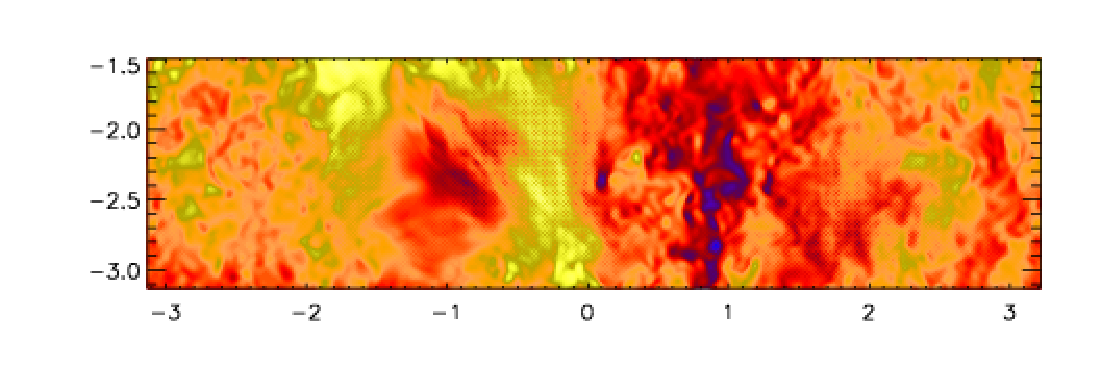
\includegraphics[width=.99\textwidth]
{timestepoverviscous}\end{center}\caption[]{
Example of a velocity slice from a run where the time step is too long.
Note the spurious checkerboard modulation in places, for example
near $x=-0.5$ and $-2.5<y<-1.5$.
This is an example of a hyperviscous turbulence simulations with
$512^3$ meshpoints and a third order hyperviscosity of
$\nu_3=5\times10^{-12}$. Hyperviscosity is explained in the
Appendix~\ref{high-freq-filters}.}\label{Ftimestepoverviscous}\end{figure}

Timestepping is accomplished using the Runge-Kutta 2N scheme.
Regarding details of this scheme see Sect.~\ref{S-2N-scheme}.

\subsubsection{The Runge-Kutta-Fehlberg time step}
\index{Runge-Kutta-Fehlberg time step}

A fifth order Runge-Kutta-Fehlberg time stepping procedure is available.
It is used mostly for chemistry application, often together with the
double precision option.
In order to make this work, you need to compile with
\begin{verbatim}
TIMESTEP  =   timestep_rkf
\end{verbatim}
in \file{src/Makefile.local}.
In addition, you must put \cmd{itorder=5} in \file{run.in}.
An example application is \file{samples/1d-tests/H2_flamespeed}.
This procedure is still experimental.

% ---------------------------------------------------------------------- %

\subsection{Boundary conditions}
\label{boundconds}
\index{Boundary conditions}

\subsubsection{Where to specify boundary conditions}
\label{S-boundconds-where}

In most tests that come with the {\sc Pencil Code}, boundary conditions are set
in \file{run.in}, which is a natural choice.
However, this may lead to unexpected initial data written by
\file{start.x}, since when you start the code (via \file{start.csh}), the
boundary conditions are unknown and \file{start.x} will then fill the ghost
zones assuming periodicity (the default boundary condition) in all three
directions.
These ghost data will never be used in a calculation, as \file{run.x} will
apply the boundary conditions before using any ghost-zone values.

To avoid these periodic conditions in the initial snapshot, you
can set the boundary conditions in \file{start.in} already.
In this case, they will be inherited by \file{run.x}, unless you also
explicitly set boundary conditions in \file{run.in}.


\subsubsection{How to specify boundary conditions}
\index{Ghost zones}

Boundary conditions are implemented through three layers of
\name{ghost points} on either boundary, which is quite a natural choice
for an MPI code that uses ghost zones for representing values located on
the neighboring processors anyway.
The desired type of boundary condition is set through the parameters
\var{bc\{x,y,z\}}
\index[var]{bcx@\emph{bcx}}%
\index[var]{bcy@\emph{bcy}}%
\index[var]{bcz@\emph{bcz}}%
in \file{run.in}; the nomenclature used is as follows.
Set \var{bc\{x,y,z\}} to a sequence of letters like
\begin{alltt}
  bcx = 'p','p','p', 'p',  'p'
\end{alltt}
for periodic boundaries, or
\begin{alltt}
  bcz = 's','s','a','a2','c1:c2'
\end{alltt}
for non-periodic ones.
Each element corresponds to one of the
variables, which are those of the variables
$u_x$, $u_y$, $u_z$, $\ln\rho$, $s/c_p$, $A_x$, $A_y$, $A_z$, $\ln c$
that are actually used \emph{in this order}.
The following conditions are available:
\begin{description}
\item[\option{p}] periodic boundary condition
\item[\option{a}] antisymmetric condition w.\,r.\,t.~the
  boundary, i.\,e.~vanishing value
\item[\option{s}] symmetric condition w.\,r.\,t.~the
  boundary, i.\,e.~vanishing first derivative
\item[\option{a2}] antisymmetry w.\,r.\,t.~the
  arbitrary value on the boundary, i.\,e.~vanishing
  second derivative
\item[\option{c1}] special boundary condition for
  $\ln\rho$ and $s$: constant heat flux through the
  boundary
\item[\option{c2}] special boundary condition for
  $s$: constant temperature at the boundary --- requires boundary
  condition \code{a2} for $\ln\rho$
\item[\option{cT}] special boundary condition for
  $s$ or $\ln\ T$: constant temperature at the boundary (for arbitrarily set
  $\ln\rho$)
\item[\option{ce}] special boundary condition for
  $s$: set temperature in ghost points to value on boundary (for
  arbitrarily set $\ln\rho$)
\item[\option{db}] low-order one-sided derivatives (``no
    boundary condition'') for density
\item[\option{she}] shearing-sheet boundary condition (default when the
  module \name{Shear} is used)
\item[\option{g}] force the value of the corresponding field on vertical
boundaries (should be used in combination with the force_lower_bound and
force_upper_bound flags set in the namelist {\it init_pars})
\item[\option{hs}] special boundary condition for $\ln\rho$ and $s$
which enforces hydrostatic equilibrium on vertical boundaries
\end{description}
The extended syntax $a$:$b$ (e.\,g.~`\code{c1:c2}') means: use
boundary condition $a$ at the left/lower boundary, but
$b$ at the right/upper one.

If you build a new \file{run.in} file from another one with a different number
of variables (\name{noentropy} vs.~\name{entropy}, for example), you need
to remember to adjust the {\it length} of the arrays \var{bcx} to \var{bcz}.
The advantage of the present approach is that it is very easy to exchange
all boundary conditions by a new set of conditions in a particular
direction (for example, make everything periodic, or switch off shearing
sheet boundary conditions and have stress-free instead).

% ---------------------------------------------------------------------- %

\subsection{Restarting a simulation}
\index{Restarting}

When a run stops at the end of a simulation, you can just resubmit
the job again, and it will start from the latest snapshot saved in
\file{data/proc*/var.dat}. The value of the latest time is saved in a
separate file, \file[time.dat]{data/proc*/time.dat}.
On parallel machines it is possible that some (or just one) of the
\file{var.dat} are corrupt; for example after a system crash.
Check for file size and date, and restart from a good \file{VAR}$N$
file instead.

If you want to run on a different machine, you just need to copy the
\file[var.dat]{data/proc*/var.dat} (and, just to be sure)
\file[time.dat]{data/proc*/time.dat}) files into a new directory tree.
You may also need the \file[seed.dat]{data/proc*/seed.dat}
files for the random number generator. The easiest way to get all these
other files is to run \cmd{start.csh} again on the new machine (or in
a new directory) and then to overwrite the
\file[var.dat]{data/proc*/var.dat} files with the correct ones.

For restarting from runs that didn't have magnetic fields, passive scalar
fields, or test fields, see Sect.~\ref{RestartingFromLessPhysics}.

% ---------------------------------------------------------------------- %

\subsection{One- and two-dimensional runs}

If you want to run two-dimensional problems, set the number
of mesh points in one direction to unity, e.g.\ \var{nygrid}=1
or \var{nzgrid}=1 in \file{cparam.local}.
Remember that the number of mesh points is still divisible by
the number of processors.
For 2D-runs, it is also possible to write only 2D-snapshots (i.e. VAR
files written only in the considered $(x,y)$ or $(x,z)$ plane, with a size
seven times smaller as we do not write the third unused direction). To
do that, please add the logical flag `lwrite_2d=T' in the namelist {\it
init_pars} in \file{start.in}.

Similarly, for one-dimensional problems, set, for example,
\var{nygrid}=1 and \var{nzgrid}=1 in \file{cparam.local}.
You can even do a zero-dimensional run, but then you better
set \var{dt} (rather than \var{cdt}), because there is no
Courant condition for the time step.

See \emph{0d, 1d, 2d, and 3d tests} with examples.

% ---------------------------------------------------------------------- %

\subsection{Visualization}
\label{S-Visualization}

\subsubsection{Gnuplot}
\label{S-gnuplot}
Simple visualization can easily be done using \name{Gnuplot}
(\url{http://www.gnuplot.info}), an open-source plotting program suitable
for two-dimensional plots.

For example, suppose you have the variables
\begin{verbatim}
  ---it-----t-------dt-------urms-----umax-----rhom-----ssm------dtc---
\end{verbatim}
in \file{time_series.dat} and want to plot $u_{\rm rms}(t)$.
Just start gnuplot and type
\begin{alltt}
  \prompt{gnuplot> } plot "data/time_series.dat" using 2:4 with lines
\end{alltt}
If you work over a slow line and want to see both  $u_{\rm rms}(t)$ and
$u_{\rm max}(t)$, use ASCII graphics:
\begin{alltt}
  \prompt{gnuplot> } set term dump
  \prompt{gnuplot> } set logscale y
  \prompt{gnuplot> } plot "data/time_series.dat" using 2:4 title "urms", \bs
  \prompt{gnuplot> }      "data/time_series.dat" using 2:5 title "umax"
\end{alltt}


\subsubsection{Data explorer}
\label{S-openDX}

\name{DX} (\name{data explorer}; \url{http://www.opendx.org}) is an
open-source tool for visualization of three-dimensional data.

The {\sc Pencil Code} provides a few networks for \name{DX}.
It is quite easy to read in a snapshot file from \name{DX} (the only
tricky thing is the four extra bytes at the beginning of the file,
representing a Fortran record marker), and whenever you run \file{start.x},
the code writes a file \file{var.general} that tells \name{DX} all it
needs to know about the data structure.

As a starting point for developing your own \name{DX} programs or
\name{networks}, you can use a few generic \name{DX} scripts provided in
the directory \file[dx/basic]{dx/basic/}.
From the run directory, start \name{DX} with
\begin{alltt}
  \prompt{unix> } dx -edit \$PENCIL_HOME/dx/basic/lnrho
\end{alltt}
to load the file \file[lnrho.net]{dx/basic/lnrho.net}, and
execute it with \key{Ctl-o} or \textsf{Execute $\rightarrow$ Execute Once}.
You will see a set of iso-surfaces of logarithmic density.
If the viewport does not fit to your data, you can reset it with
\key{Ctl-f}.
To rotate the object, drag the mouse over the Image window with the left or
right mouse button pressed.
Similar networks are provided for entropy (\file{ss.net}), velocity
(\file{uu.net}) and magnetic field (\file{bb.net}).

When you expand these simple networks to much more elaborate ones, it is
probably a good idea to separate the different tasks (like Importing and
Selecting, visualizing velocity, visualizing entropy, and Rendering) onto
separate pages through \textsf{Edit $\rightarrow$ Page}.


\paragraph{Note}
Currently, \name{DX} can only read in data files written by one single
processor, so from a multi-processor run, you can only visualize one
subregion at a time.


\subsubsection{GDL}
\label{S-GDL}
\name{GDL}, also known as \name{Gnu Data Language} is a free visualization
package that can be found at
\url{http://gnudatalanguage.sourceforge.net/}.
It aims at replacing the very expensive \name{IDL} package (see
S.~\ref{S-IDL-routines}).
For the way we use IDL for the Pencil Code, compatibility is currently not
completely sufficient, but you can use GDL for many of the visualization
tasks.
If you get spurious ``Error opening file'' messages, you can normally
simply ignore them.

This section tells you how to get started with using GDL for visualization.

\paragraph{Setup}
\index{Setup}
As of GDL 0.9 -- at least the version packed with Ubuntu Jaunty (9.10) --
you will need to add GDL's \file{examples/pro/} directory to your
\var{!PATH} variable.
So the first call after starting \name{GDL} should be
\begin{alltt}
  \prompt{GDL> } .run setup_gdl
\end{alltt}

\paragraph{Starting visualization}
There are mainly two possibilities for visualization: using a simple GUI
or loading the data with \code{pc_read} and work with it interactively.
Please note that the GUI was written and tested only with IDL, see
\S\ref{S-IDL-visualization}.

Here, the \code{pc_read} family of IDL routines to read the data is described.
Try
\begin{alltt}
  \prompt{GDL> } pc_read
\end{alltt}
to get an overview.

To plot a time series, use
\begin{alltt}
  \prompt{GDL> } pc_read_ts, OBJECT=ts
  \prompt{GDL> } help, ts, /STRUCT  ;; (to see which slots are available)
  \prompt{GDL> } plot, ts.t, ts.umax
  \prompt{GDL> } oplot, ts.t, ts.urms
\end{alltt}
Alternatively, you could simply use the \file{ts.pro} script:
\begin{alltt}
  \prompt{GDL> } .run ts
\end{alltt}

To work with data from \file{var.dat} and similar snapshot files, you can
e.g. use the following routines:
\begin{alltt}
  \prompt{GDL> } pc_read_dim, OBJECT=dim
  \prompt{GDL> } $$PENCIL_HOME/bin/nl2idl -d -m ./data/param.nml> ./param.pro
  \prompt{GDL> } pc_read_param, OBJECT=par
  \prompt{GDL> } pc_read_grid, OBJECT=grid
  \prompt{GDL> } pc_read_var, OBJECT=var
\end{alltt}
Having thus read the data structures, we can have a look at them to see
what information is available:
\begin{alltt}
  \prompt{GDL> } help, dim, /STRUCT
  \prompt{GDL> } help, par, /STRUCT
  \prompt{GDL> } help, grid, /STRUCT
  \prompt{GDL> } help, var, /STRUCT
\end{alltt}

To visualize data, we can e.g. do\footnote{
  If \code{contourfill} produces just contour lines instead of a
  color-coded plot, your version of GDL is too old.
  E.g. the version shipped with Ubuntu 9.10 is based on GDL 0.9rc1 and has
  this problem.
}
\begin{alltt}
  \prompt{GDL> } plot, grid.x, var.ss[*, dim.ny/2, dim.nz/2]
  \prompt{GDL> } contourfill, var.ss[*, *, dim.nz/2], grid.x, grid.y

  \prompt{GDL> } ux_slice = var.uu[*, *, dim.nz/2, 0]
  \prompt{GDL> } uy_slice = var.uu[*, *, dim.nz/2, 1]
  \prompt{GDL> } wdvelovect, ux_slice, uy_slice, grid.x, grid.y

  \prompt{GDL> } surface, var.lnrho[*, *, dim.nz/2, 0]
\end{alltt}

See also Sect.~\ref{S-IDL-routines}.


\subsubsection{IDL}
\label{S-IDL-routines}

\name{IDL} is a commercial visualization program for two-dimensional and
simple three-dimensional graphics.
It allows to access and manipulate numerical data in a fashion quite
similar to how Fortran handles them.

In \file[idl/]{\$PENCIL_HOME/idl}, we provide a number of general-purpose
\name{IDL} scripts that we are using all the time in connection with the
{\sc Pencil Code}.
While \name{IDL} is quite an expensive software package, it is quite
useful for visualizing results from numerical simulations.
In fact, for many applications, the 7-minute demo version of \name{IDL} is
sufficient.

\paragraph{Visualization in IDL}
\label{S-IDL-visualization}
The Pencil Code GUI is a data post-processing tool for the usage on a
day-to-day basis. It allows fast inspection of many physical quantities,
as well as advanced features like horizontal averages, stramline tracing,
freely orientable 2D-slices, and extraction of cut images and movies.
To use the Pencil Code GUI, it is sufficient to run:
\begin{alltt}
  \prompt{unix> } idl
  \prompt{IDL> }  .r pc_gui
\end{alltt}
If you like to load only some subvolume of the data, like any 2D-slices
from the given data snapshots, or 3D-subvolumes, it is possible to choose
the corresponding options in the file selector dialog.
The Pencil Code GUI offers also some options to be set on the command-line,
please refer to their description in the source code.

There are also other small GUIs available, e.g. the file `time-series.dat'
can easily be analysed with the command:
\begin{alltt}
  \prompt{unix> } idl
  \prompt{IDL> }  pc_show_ts
\end{alltt}

The easiest way to derive physical quantities at the command-line is to use
one of the many \cmd{pc_read_var}-variants (\cmd{pc_read_var_raw} is
recommended for large datasets because of its high efficiency regarding
computation and memory usage) for reading the data. With that, one can make
use of \cmd{pc_get_quantity} to derive any implemented physical quantity.
Packed in a script, this is the recommended way to get reproducible results,
without any chance for accidental errors on the interactive IDL command-line.

Alternatively, by using the command-line to see the time evolution of e.g.
velocity and magnetic field (if they are present in you run), start \name{IDL}
\footnote{
  If you run IDL from the command line, you will highly appreciate the
  following tip:
  IDL's command line editing is broken beyond hope.
  But you can fix it, by running IDL under \cmd{rlwrap}, a wrapper for the
  excellent GNU \name{readline} library.

\index{Download}
  Download and install \cmd{rlwrap} from
  \path{http://utopia.knoware.nl/~hlub/uck/rlwrap/} (on some systems you
  just need to run `\code{emerge rlwrap}', or `\code{apt-get install
    rlwrap}'), and alias your \cmd{idl} command:
\begin{alltt}
  \ \ \ \ \prompt{csh> } \ alias idl 'rlwrap -a -c idl'
\end{alltt}
\begin{alltt}
  \ \ \ \ \prompt{bash> } alias idl='rlwrap -a -c idl'
\end{alltt}

  From now on, you can
  \begin{itemize}
  \setlength{\itemsep}{-0.5\parsep}
  \item use long command lines that correctly wrap around;
  \item type the first letters of a command and then \key{PageUp} to recall
    commands starting with these letters;
  \item capitalize, uppercase or lowercase a word with \key{Esc}-C,
    \key{Esc}-U, \key{Esc}-L;
  \item use command line history across IDL sessions (you might
    need to create \file{\~{}/.idl_history} for this);
  \item complete file names with \key{Tab} (works to some extent);
  \item \ldots use all the other \name{readline} features that you are
    using in \cmd{bash}, \cmd{octave}, \cmd{bc}, \cmd{gnuplot},
    \cmd{ftp}, etc.
  \end{itemize}
}
and run \file{ts.pro}:
\begin{alltt}
  \prompt{unix> } idl
  \prompt{IDL> }  .run ts
\end{alltt}
The \name{IDL} script \file{ts.pro} reads the time series data from
\file[time_series.dat]{data/time_series.dat} and sorts the column into
the structure \var{ts}, with the slot names corresponding to the
name of the variables (taken from the header line of
\file[time_series.dat]{data/time_series.dat}).
Thus, you can refer to time as \code{ts.t}, to the rms velocity as
\code{ts.urms}, and in order to plot the mean density as a function of
time, you would simply type
\begin{alltt}
  \prompt{IDL> } plot, ts.t, ts.rhom
\end{alltt}

\bigskip

The basic command sequence for working with a snapshot is:
\begin{alltt}
  \prompt{unix> } idl
  \prompt{IDL> }  .run start
  \prompt{IDL> }  .run r
  \prompt{IDL> }  {\sl[specific commands]} \
\end{alltt}
You run \file{start.pro} once to initialize (or reinitialize,
if the mesh size has changed, for example) the fields and read in the
startup parameters from the code.
To read in a new snapshot, run \file{r.pro} (or \file{rall.pro}, see below).

If you are running in parallel on several processors,
the data are scattered over different directories.
To reassemble everything in \name{IDL}, use
\begin{alltt}
  \prompt{IDL> } .r rall
\end{alltt}
instead of \cmd[.run]{.r r}
(here, \cmd[.run]{.r} is a shorthand for \cmd{.run}).
The procedure \file{rall.pro} reads (and assembles) the data from all
processors and correspondingly requires large amounts of memory
for very large runs.
If you want to look at just the data from one processor, use \file{r.pro}
instead.

If you need the magnetic field or the current density, you can calculate
them in IDL by \footnote{
  Keep in mind that \code{jj=curl(bb)} would use iterated first derivatives
  instead of the second derivatives and thus be numerically less accurate
  than \code{jj=curl2(aa)}, particularly at small scales.
}
\begin{alltt}
  \prompt{IDL> } bb=curl(aa)
  \prompt{IDL> } jj=curl2(aa)
\end{alltt}

By default one is reading always the current snapshot
\file[var.dat]{data/proc$N$/var.dat}; if you want to read one of the
permanent snapshots, use (for example)
\begin{alltt}
  \prompt{IDL> } varfile='VAR2'
  \prompt{IDL> } .r r {\sl(or \texttt{.r rall})}
\end{alltt}
See Sect.~\ref{snapshots} for details on permanent snapshots.

With \file{r.pro}, you can switch the part of the domain by changing the
variable \var{datadir}:
\begin{alltt}
  \prompt{IDL> } datadir='data/proc3'
  \prompt{IDL> } .r r
\end{alltt}
will read the data written by processor 3.

\paragraph{Reading data into IDL arrays or structures}

As an alternative to the method described above, there is also the possibility
to read the data into structures. This makes some more operations possible,
e.g.\ reading data from an IDL program where the command \cmd{.r} is not
allowed.

An efficient and still scriptable way would look like the following:
\begin{alltt}
  \prompt{IDL> } pc_read_var_raw, obj=var, tags=tags
  \prompt{IDL> } bb = pc_get_quantity ('B', var, tags)
  \prompt{IDL> } jj = pc_get_quantity ('j', var, tags)
\end{alltt}
This reads the data into an array `var', as well as the array indices of the
contained physical variables into a separate structure `tags'.
To use a caching mechanism withhin \cmd{pc_get_quantity}, please refer to
the documentation and the examples contained in `pencil-code/idl/pc_get_quantity.pro',
where you can also start adding not yet implemented physical quantities.

To read a snapshot \cmd{'VAR10'} into the IDL structure \cmd{ff}, type the
following command
\begin{alltt}
  \prompt{IDL> } pc_read_var, obj=ff, varfile='VAR10', /trimall
\end{alltt}
The option \cmd{/trimall} removes ghost zones from the data. A number of other
options are documented in the source code of \cmd{pc_read_var}. You can see
what data the structure contains by using the command \cmd{tag_names}
\begin{alltt}
  \prompt{IDL> } print, tag_names(ff)
  T X Y Z DX DY DZ UU LNRHO AA
\end{alltt}
One can access the individual variables by typing \cmd{ff.varname}, e.g.
\begin{alltt}
  \prompt{IDL> } help, ff.aa
  <Expression>    FLOAT     = Array[32, 32, 32, 3]
\end{alltt}
There are a number of files that read different data into structures. They are
placed in the directory \cmd{\$PENCIL_HOME/idl/files}. Here is a list of files
(including suggested options to call them with)
\begin{itemize}
  \item \cmd{pc_read_var_raw, obj=var, tags=tags} \\
      Efficiently read a snapshot into an array.
  \item \cmd{pc_read_var, obj=ff, /trimall} \\
      Read a snapshot into a structure.
  \item \cmd{pc_read_ts, obj=ts} \\
      Read the time series into a structure.
  \item \cmd{pc_read_xyaver, obj=xya} \\
      \cmd{pc_read_xzaver, obj=xza} \\
      \cmd{pc_read_yzaver, obj=yza} \\
      Read 1-D time series into a structure.
  \item \cmd{pc_read_const, obj=cst} \\
      Read code constants into a structure.
  \item \cmd{pc_read_pvar, obj=fp} \\
      Read particle data into a structure.
  \item \cmd{pc_read_param, obj=par} \\
      Read startup parameters into a structure.
  \item \cmd{pc_read_param, obj=par2, /param2} \\
      Read runtime parameters into a structure.
\end{itemize}
Other options are documented in the source code of the files.

For some examples on how to use these routines, see Sect.~\ref{S-GDL}.

\subsubsection{Python}
\label{Python}

Pencil also supports visualization using \name{python}. A number of scripts
for such are placed in the subfolder \file{\$PENCIL_HOME/python}. A
README file placed under that subfolder contains the information
needed to read Pencil output data into python.

To start rapidly under Python:

\begin{enumerate}

\item you must install the matplotlib library (a package often called
   python-matplotlib)
\item normally, numpy is installed as a dependency
\item the PYTHONPATH is initialised when sourcing 'sourceme.*'
\item for us, the best practical way to use Python is to start the ipython
   shell so its installation is a good idea
\item you must load all of the Python pencil modules using 'import pencil
   as pc'
\item you run a module using 'pc.read_ts()' and so on...

\end{enumerate}

% ---------------------------------------------------------------------- %

\subsection{Running on multi-processor computers}
\label{MPI}

The code is parallelized using \name{MPI} (\dfn{message passing
interface}) for a simple domain decomposition (data-parallelism), which is
a straight-forward and very efficient way of parallelizing
finite-difference codes.
The current version has a few restrictions, which need to be kept in mind
when using the MPI features.

First, only the $y$ and $z$ directions can be distributed over different
processors.
Second, the global number of grid points (but excluding the ghost zones)
in a given direction must be an exact multiple of the number of processors
you use in that direction.
For example if you have \code{nprocy=8} processors for the $y$ direction, you
can run a job with \code{nygrid=64} points in that direction, but if you
try to run a problem with \code{nygrid=65} or \code{nygrid=94}, the code
will complain about an inconsistency and stop.
(So far, this has not been a serious restriction for us.)

\subsubsection{How to run a sample problem in parallel}

To run the sample problem in the directory
\file[conv-slab/]{samples/conv-slab} on 16
CPUs, you need to do the following (in that directory):

\begin{enumerate}

\item Edit \file[Makefile.local]{src/Makefile.local} and replace
  \begin{alltt}
  MPICOMM   = nompicomm \
  \end{alltt}
  by
  \begin{alltt}
  MPICOMM   =   mpicomm \
  \end{alltt}

\item Edit \file[cparam.local]{src/cparam.local} and replace
  \begin{alltt}
  integer, parameter :: ncpus=1,nprocy=1,nprocz=ncpus/nprocy,nprocx=1
  integer, parameter :: nxgrid=32,nygrid=nxgrid,nzgrid=nxgrid \
  \end{alltt}
  by
  \begin{alltt}
  integer, parameter :: ncpus=16,nprocy=4,nprocz=ncpus/nprocy,nprocx=1
  integer, parameter :: nxgrid=128,nygrid=nxgrid,nzgrid=nxgrid \
  \end{alltt}
  The first line specifies a $4{\times}4$ layout of the data in the $y$
  and $z$ direction.
  The second line increases the resolution of the run because
  running a problem as small as $32^3$ on 16 CPUs would be wasteful.
  Even $128^3$ may still be quite small in that respect.
  For performance timings, one should try and keep the size of the
  problem per CPU the same, so for example $256^3$ on 16 CPUs should
  be compared with $128^3$ on 2 CPUs.

\item Recompile the code
  \begin{alltt}
  \prompt{unix> } (cd src; make)
  \end{alltt}

\item Run it
  \begin{alltt}
  \prompt{unix> } start.csh
  \prompt{unix> } run.csh
  \end{alltt}

\end{enumerate}

Make sure that all CPUs see the same \file{data/} directory; otherwise
things will go wrong.

Remember that in order to visualize the full domain with IDL (rather than
just the domain processed and written by one processor), you need to use
\file{rall.pro} instead of \file{r.pro}.

\subsubsection{Hierarchical networks (e.g.~on Beowulf clusters)}
\label{Bandwidth}
\index{bandwidth}
\index{Beowulf clusters}

On big Beowulf clusters, a group of nodes is often connected with a switch
of modest speed, and all these groups are connected via a $n$ times
faster uplink switch.
When bandwidth-limited, it is important to make sure that
consecutive processors are mapped onto the mesh such that the load on
the uplink is $\lesssim n$ times larger than the load on the
slower switch within each group.
On a 512 node cluster, where groups of 24 processors are linked via fast
ethernet switches, which in turn are connected via a Gigabit uplink
($\sim10$ times faster), we found that \var{nprocy}=4 is optimal.
For 128 processors, for example we find that
$\var{nprocy}\times\var{nprocz}=4\times32$ is the optimal layout, while.
For comparison, $8\times16$ is 3 times slower, and $16\times8$
is 17 (!) times slower.
These results can be understood from the structure of the network, but the
basic message is to watch out for such effects and to try varying
\var{nprocy} and \var{nprocz}.

In cases where \code{nygrid}$>$\code{nzgrid} it may be advantageous to
swap the ordering of processor numbers.
This can be done by setting \var{lprocz_slowest}=\code{F}.

\subsubsection{Extra workload caused by the ghost zones}
\index{Ghost zones}

Normally, the workload caused by the ghost zones is negligible.
However, if one increases the number of processors, a significant
fraction of work is done in the ghost zones.
In other words, the effective mesh size becomes much larger than
the actual mesh size.

Consider a mesh of size $N_w=N_x\times N_y\times N_z$,
and distribute the task over $P_w=P_x\times P_y\times P_z$ processors.
If no communication were required, the number of points per processor
would be
\begin{equation}
{N_w\over P_w}={N_x\times N_y\times N_z\over P_x\times P_y\times P_z}.
\end{equation}
However, for finite difference codes some communication is required,
and the amount of communication depends on spatial order of the
scheme, $Q$.
The {\sc Pencil Code} works by default with sixth order finite differences,
so $Q=6$, i.e.\ one needs 6 ghost zones, 3 on each end of the mesh.
With $Q\neq0$ the number of points per processor is
\begin{equation}
{N_w^{\rm(eff)}\over P_w}=
\left({N_x\over P_x}+Q\right)\times
\left({N_y\over P_y}+Q\right)\times
\left({N_z\over P_z}+Q\right).
\end{equation}
There is efficient scaling only when
\begin{equation}
\min\left({N_x\over P_x}, {N_y\over P_y}, {N_z\over P_z}\right)\gg Q.
\end{equation}
In the special case were $N_x=N_y=N_z\equiv N=N_w^{1/3}$,
with $P_x=1$ and $P_y=P_z\equiv P=P_w^{1/2}$, we have
\begin{equation}
{N_w^{\rm(eff)}\over P_w}=
\left(N+Q\right)\times
\left({N\over P}+Q\right)^2.
\end{equation}
For $N=128$ and $Q=6$ the effective mesh size exceeds the actual mesh
size by a factor
\begin{equation}
{N_w^{\rm(eff)}\over N_w}
=\left(N+Q\right)\times\left({N\over P}+Q\right)^2\times{P_w\over N_w}.
\end{equation}
These factors are listed in Table~\ref{EffectiveMesh}.

\begin{table}[h!]\caption{
$N_w^{\rm(eff)}/N_w$ versus $N$ and $P$.
}\vspace{12pt}\centerline{\begin{tabular}{rrrrrrrrrrrr}
$P\backslash N$ &    128  &    256  &    512  &   1024  &   2048 \\
\hline
    1  &   1.15  &   1.07  &   1.04  &   1.02  &   1.01 \\
    2  &   1.19  &   1.09  &   1.05  &   1.02  &   1.01 \\
    4  &\underline{1.25}&   1.12  &   1.06  &   1.03  &   1.01 \\
    8  &   1.34  &   1.16  &   1.08  &   1.04  &   1.02 \\
   16  &   1.48  &\underline{1.22}&   1.11  &   1.05  &   1.03 \\
   32  &   1.68  &   1.31  &   1.15  &   1.07  &   1.04 \\
   64  &   1.98  &   1.44  &\underline{1.21}&   1.10  &   1.05 \\
  128  &   2.45  &   1.64  &   1.30  &   1.14  &   1.07 \\
  256  &   3.21  &   1.93  &   1.43  &\underline{1.20}&   1.10 \\
  512  &   4.45  &   2.40  &   1.62  &   1.29  &   1.14 \\
\label{EffectiveMesh}\end{tabular}}\end{table}

Ideally, one wants to keep the work in the ghost zones at a minimum.
If one accepts that 20--25\% of work are done in the ghost zones,
one should use 4 processors for $128^3$ mesh points,
16 processors for $256^3$ mesh points,
64 processors for $512^3$ mesh points,
256 processors for $1024^3$ mesh points,
and 512 processors for $1536^3$ mesh points.

%\begin{figure}[h!]\begin{center}
%\includegraphics[width=\columnwidth]{figs/processor_scaling}
%\end{center}\caption[]{
%Scaling
%}\label{pcoolheat}\end{figure}

% ---------------------------------------------------------------------- %

\subsection{Running in double-precision}
\label{double-precision}
\index{double precision}

With many compilers, you can easily switch to double precision (8-byte
floating point numbers) as follows.

Add the lines
\begin{alltt}
  # Use double precision
  REAL_PRECISION = double
\end{alltt}
to \file[Makefile.local]{src/Makefile.local} and (re-)run
\cmd{pc_setupsrc}.

If \var{REAL_PRECISION} is set to `double', the flag \var{FFLAGS_DOUBLE}
is appended to the Fortran compile flags.
The default for \var{FFLAGS_DOUBLE} is \code{-r8}, which works for
\name{g95} or \cmd{ifort}; for \name{gfortran}, you need to make sure that
\var{FFLAGS_DOUBLE} is set to \code{-fdefault-real-8}.

You can see the flags in \file{src/Makefile.inc}, which is the first place
to check if you have problems compiling for double precision.

\medskip

Using double precision might be important in turbulence runs where
the resolution is $256^3$ meshpoints and above (although such runs
often seem to work fine at single precision).
The procedure \file[realtodouble.x]{postproc/src/realtodouble.x} can be
used to convert existing
\file{var.dat} and \file{grid.dat} files to double precision.

% ---------------------------------------------------------------------- %

\subsection{Power spectrum}
\label{power-spectrum}
Given a real variable $u$, its Fourier transform $\tilde{u}$
is given by
\begin{eqnarray}
  \tilde{u}(k_x,k_y,k_z)
  \ =\ \mathcal{F}(u(x,y,z))
  &=& \frac{1}{N_x N_y N_z} \sum_{p=0}^{N_x-1} \sum_{q=0}^{N_y-1}
       \sum_{r=0}^{N_z-1} u(x_p,y_q,z_r)  \nonumber \\
  & & {} \times \exp(-i k_x  x_p) \exp(-i k_y y_q)
         \exp(-i k_z z_r) ,
\end{eqnarray}
where
\[
   |k_x| < \frac{\pi N_x}{L_x} \, ,\qquad
   |k_y| < \frac{\pi N_y}{L_y} \, ,\qquad
   |k_z| < \frac{\pi N_z}{L_z} \, ,
\]
when $L$ is the size of the simulation box.
The three-dimensional power spectrum $P(k)$ is defined as
\begin{equation}
  P(k)=\frac{1}{2}\tilde{u}\tilde{u}^*,
\end{equation}
where
\begin{equation}
  k=\sqrt{k_x^2+k_y^2+k_z^2} .
\end{equation}
Note that we can only reasonably calculate $P(k)$ for $k < \pi N_x/L_x$.

To get power spectra from the code, edit \file{run.in} and add for example
the following lines
\begin{alltt}
  dspec=5., ou_spec=T, ab_spec=T !(for energy spectra)
  oned=T
\end{alltt}
under \code{run_pars}.
The kinetic (\code{vel_spec}) and magnetic  (\code{mag_spec}) power spectra
will now be calculated every 5.0 (\code{dspec}) time units.
The Fourier spectra is calculated using \name{fftpack}.
In addition to calculating the three-dimensional
power spectra also the one-dimensional power spectra will be calculated
(\code{oned}).

In addition one must edit
\file[Makefile.local]{src/Makefile.local} and add the lines
\begin{alltt}
   FOURIER=fourier_fftpack
   POWER=power_spectrum
\end{alltt}

Running the code will now create the files \file{powerhel_mag.dat} and
\file{power_kin.dat} containing the three-dimensional
magnetic and kinetic power spectra respectively. In addition to these
three-dimensional files we will also find the one-dimensional files
\file{powerbx_x.dat},
\file[powerbx_x.dat]{powerby_x.dat}, % one index entry is enough..
\file[powerbx_x.dat]{powerbz_x.dat},
\file{powerux_x.dat},
\file[powerux_x.dat]{poweruy_x.dat} and
\file[powerux_x.dat]{poweruz_x.dat}.
In these files the data are stored such that the first line contains the
time of the snapshot, the following $\var{nxgrid}/2$ numbers represent the
power at each wavenumber, from the smallest to the largest.
If several snapshots have been saved, they are being stored immediately
following the preceding snapshot.

You can read the results with the idl procure \file{power}, like this:
\begin{alltt}
  power,'_kin','_mag',k=k,spec1=spec1,spec2=spec2,i=n,tt=t,/noplot
  power,'hel_kin','hel_mag',k=k,spec1=spec1h,spec2=spec2h,i=n,tt=t,/noplot
\end{alltt}

If powerhel is invoked, krms is written during the first computation.
The relevant output file is \file{power_krms.dat}.
This is needed for a correct calculation of $k$ used in the realizability
conditions.

A caveat of the implementation of Fourier transforms in the {\sc Pencil
Code} is that, due to the parallelization, the permitted resolution
is limited to the case when one direction is an integer multiple of
the other. So, it can be done for

\code{Nx = n*Ny}

Unfortunately, for some applications one wants \code{Nx < Ny}. Wlad experimented
with arbitrary resolution by interpolating $x$ to the same resolution of $y$
prior to transposing, then transform the interpolated array and then
interpolating it back (check \file{fourier_transform_y} in
\file{fourier_fftpack.f90}).

To visualize with \name{IDL} just type
\cmd{power} and you get the last snapshot of the three-dimensional
power spectrum. See head of \file[power.pro]{\$PENCIL_HOME/idl/power.pro}
for options to \cmd{power}.

% ---------------------------------------------------------------------- %

\subsection{Structure functions}
\label{structure-functions}
We define the p-th order longitudinal structure function of $\vec{u}$ as
\begin{equation}
S^p_{\rm long}(l)=\left< | u_x(x{+}l,y,z)-u_x(x,y,z)|^p \right> \; ,
\end{equation}
while the transversal is
\begin{equation}
S^p_{\rm trans}(l)= \left< | u_y(x{+}l,y,z)-u_y(x,y,z)|^p \right>
               + \left< | u_z(x{+}l,y,z)-u_z(x,y,z)|^p \right> \; .
\end{equation}

Edit \file{run.in} and add for example the following lines
  \begin{alltt}
  dspec=2.3,
  lsfu=T,lsfb=T,lsfz1=T,lsfz2=T
  \end{alltt}
under \code{run_pars}.
The velocity (\code{lsfu}), magnetic (\code{lsfb}) and Elsasser
(\code{lsfz1} and \code{lsfz2}) structure functions will
now be calculated every 2.3 (\code{dspec}) time unit.

In addition one must edit
\file[Makefile.local]{src/Makefile.local} and add the line
  \begin{alltt}
  STRUCT_FUNC  = struct_func
  \end{alltt}
You should also make sure that \var{nxgrid}=\var{nygrid}=\var{nzgrid}.

Running the code will now create the files: \\
\file{sfu-1.dat},
\file[sfu-1.dat]{sfu-2.dat},    % one index entry is enough
\file[sfu-1.dat]{sfu-3.dat} (velocity), \\
\file{sfb-1.dat},
\file[sfb-1.dat]{sfb-2.dat},
\file[sfb-1.dat]{sfb-3.dat} (magnetic field), \\
\file{sfz1-1.dat},
\file[sfz1-1.dat]{sfz1-2.dat},
\file[sfz1-1.dat]{sfz1-3.dat} (first Elsasser variable), \\
\file[sfz1-1.dat]{sfz2-1.dat},
\file[sfz1-1.dat]{sfz2-2.dat},
\file[sfz1-1.dat]{sfz2-3.dat} (second Elsasser variable), \\
which contains the data of interest.
The first line in each file contains the time $t$
and the number \var{qmax}, such that the largest moment
calculated is $\var{qmax}-1$.
The next \var{imax} numbers represent the first moment
structure function for the first snapshot, here
\begin{equation}
\var{imax}=2\frac{\ln (\var{nxgrid})}{\ln 2}-2.
\end{equation}
The next \var{imax} numbers contain the second moment structure function,
and so on until $\var{qmax}-1$.
The following \var{imax} numbers then contain the data of the
{\it signed} third order structure function i.e.
$S^3_{\rm long}(l)=\left< [u_x(x{+}l,y,z)-u_x(x,y,z)]^3 \right>$.

The following $\var{imax} \times \var{qmax} \times 2$ numbers are zero if
$\var{nr_directions}=1$
(default), otherwise they are the same data as above but for the
structure functions calculated in the y and z directions.

If the code has been run long enough as to calculate several snapshots, these
snapshots will now follow, being stored in the same way as the first snapshot.

To visualize with \name{IDL} just type
\cmd{structure} and you get the time-average of the first order longitudinal
structure function (be sure that
\file[forced/idl/]{pencil-runs/forced/idl/} is in \env{IDL_PATH}).
See head of \file[structure.pro]{pencil-runs/forced/idl/structure.pro}
for options to \cmd{structure}.

% ---------------------------------------------------------------------- %

\subsection{Particles}

The {\sc Pencil Code} has modules for tracer particles and for dust particles
(see Sect.~\ref{S-particles-equations}). The particle modules are chosen by
setting the value of the variable \code{PARTICLES} in \code{Makefile.local} to
either \code{particles_dust} or \code{particles_tracers}. For the former case
each particle has six degrees of freedom, three positions and three
velocities. For the latter it suffices to have only three position variables
as the velocity of the particles are equal to the instantaneous fluid velocity
at that point. In addition one can choose to have several additional internal
degrees of freedoms for the particles. For example one can temporally evolve
the particles radius by setting \code{PARTICLES_RADIUS} to
\code{particles_radius} in \code{Makefile.local}.  

All particle infrastructure is controlled and organized by the
\code{Particles_main} module. This module is automatically selected by
\code{Makefile.src} if \code{PARTICLES} is different from \code{noparticles}.
Particle modules are compiled as a separate library. This way the main part of
the Pencil Code only needs to know about the \code{particles_main.a} library,
but not of the individual particle modules.
 
For a simulation with particles one must in addition define a few parameters in
\code{cparam.local}. Here is a sample of \code{cparam.local} for a parallel run
with 2,000,000 particles:
\begin{verbatim}
integer, parameter :: ncpus=16, nprocy=4, nprocz=4, nprocx=1
integer, parameter :: nxgrid=128, nygrid=256, nzgrid=128
integer, parameter :: npar=2000000, mpar_loc=400000, npar_mig=1000
integer, parameter :: npar_species=2
\end{verbatim}
The parameter \code{npar} is the number of particles in the simulation,
\code{mpar_loc} is the number of particles that is allowed on each processor
and \code{npar_mig} is the number of particles that are allowed to migrate from
one processor to another in any time-step. For a non-parallel run it is enough
to specify \code{npar}. The number of particle species is set through
\code{npar_species} (assumed to be one if not set). The particle input
parameters are given in \code{start.in} and \code{run.in}. Here is a sample of
the particle part of \code{start.in} for dust particles:
\begin{verbatim}
/
&particles_init_pars
  initxxp='gaussian-z', initvvp='random'
  zp0=0.02, delta_vp0=0.01, eps_dtog=0.01, tausp=0.1
  lparticlemesh_tsc=T
/
\end{verbatim}
The initial positions and velocities of the dust particles are set in
\code{initxxp} and \code{initvvp}. The next four input parameters are further
specifications of the initial condition. Interaction between the particles and
the mesh, e.g.\ through drag force or self-gravity, require a mapping of the
particles on the mesh. The {\sc Pencil Code} currently supports NGP (Nearest
Grid Point, default), CIC (Cloud in Cell, set \code{lparticlemesh_cic=T}) and
TSC (Triangular Shaped Cloud, set \code{lparticlemesh_tsc=T}). See Youdin \&
Johansen (2007) for details.

Here is a sample of the particle part of \code{run.in} (also for dust
particles):
\begin{verbatim}
/
&particles_run_pars
  ldragforce_gas_par=T
  cdtp=0.2
/
\end{verbatim}
The logical \code{ldragforce_gas_par} determines whether the dust particles
influence the gas with a drag force. \code{cdtp} tells the code how many
friction times should be resolved in a minimum time-step.

The sample run \file{samples/sedimentation/} contains the latest setup for dust
particles.

\subsubsection{Particles in parallel}

The particle variables (e.g. $\vec{x}_i$ and $\vec{v}_i$) are kept in the
arrays \code{fp} and \code{dfp}. For parallel runs, particles must be able to
move from processor to processor as they pass out of the $(x,y,z)$-interval of
the local processor. Since not all particles are present at the same processor
at the same time (hopefully), there is some memory optimization in making
\code{fp} not big enough to contain all the particles at once. This is achieved
by setting the code variable \code{mpar_loc} less than \code{npar} in
\code{cparam.local} for parallel runs. When running with millions of particles,
this trick is necessary to keep the memory need of the code down.

The communication of migrating particles between the processors happens as
follows (see the subroutine \code{redist_particles_procs} in
\code{particles_sub.f90}):
\begin{enumerate}
  \item In the beginning of each time-step all processors check if any of their
  particles have crossed the local $(x,y,z)$-interval. These particles are
  called migrating particles. A run can have a maximum of \code{npar_mig}
  migrating particles in each time-step. The value of \code{npar_mig} must be
  set in \code{cparam.local}. The number should (of course) be slightly larger
  than the maximum number of migrating particles at any time-step during the
  run. The diagnostic variable \code{nmigmax} can be used to output the maximum
  number of migrating particles at a given time-step. One can set
  \code{lmigration_redo=T} in \code{\&particles_run_pars} to force the code to
  redo the migration step if more than \code{npar_mig} want to migrate. This
  does slow the code down somewhat, but has the benefit that the code does not
  stop when more than \code{npar_mig} particles want to migrate.
  \item The index number of the receiving processor is then calculated. This
  requires some assumption about the grid on other processors and will
  currently not work for nonequidistant grids. Particles do not always pass to
  neighboring processors as the global boundary conditions may send them to the
  other side of the global domains (periodic or shear periodic boundary
  conditions).
  \item The migrating particle information is copied to the end of $\code{fp}$,
  and the empty spot left behind is filled up with the particle of the highest
  index number currently present at the processor.
  \item Once the number of migrating particles is known, this information is
  shared with neighboring processors (including neighbors over periodic
  boundaries) so that they all know how many particles they have to receive and
  from which processors.
  \item The communication happens as directed MPI communication. That means
  that processors 0 and 1 can share migrating particles at the same time as
  processors 2 and 3 do it. The communication happens from a chunk at the end
  of \code{fp} (migrating particles) to a chunk that is present just after the
  particle of the highest index number that is currently at the receiving
  processor. Thus the particles are put directly at their final destination,
  and the migrating particle information at the source processor is simply
  overwritten by other migrating particles at the next time-step.
  \item Each processor keeps track of the number of particles that it is
  responsible for. This number is stored in the variable \code{npar_loc}.  It
  must never be larger than \code{mpar_loc} (see above). When a particle
  leaves a processor, \code{npar_loc} is reduced by one, and then increased by
  one at the processor that receives that particle. The maximum number of
  particles at any processor is stored in the diagnostic variable
  \code{nparmax}. If this value is not close to \code{npar}/\code{ncpus}, the
  particles have piled up in such a way that computations are not evenly shared
  between the processors. One can then try to change the parallelization
  architecture (\code{nprocy} and \code{nprocz}) to avoid this problem.
\end{enumerate}

In simulations with many particles (comparable to or more than the number of
grid cells), it is crucial that particles are shared relatively evenly among
the processors. One can as a first approach attempt to not parallelize
directions with strong particle density variations. However, this is often not
enough, especially if particles clump locally.

Alternatively one can use Particle Block Domain Decomposition (PBDD, see
Johansen et al.\ 2011). The steps in Particle Block Domain Decomposition scheme
are as follows:
\begin{enumerate}
  \item The fixed mesh points are domain-decomposed in the usual way (with
  \code{ncpus}=\code{nprocx}$\times$\code{nprocy}$\times$\code{nprocz}).
  \item Particles on each processor are counted in {\it bricks} of size \code{
  nbx}$\times$\code{nby}$\times$\code{nbz} (typically \code{nbx}$=$\code{
  nby}$=$\code{nbz}$=$\code{4}).
  \item Bricks are distributed among the processors so that each processor has
  approximately the same number of particles
  \item Adopted bricks are referred to as {\it blocks}.
  \item The Pencil Code uses a third order Runge-Kutta time-stepping scheme. In
  the beginning of each sub-time-step particles are counted in blocks and the
  block counts communicated to the bricks on the parent processors. The
  particle density assigned to ghost cells is folded across the grid, and the
  final particle density (defined on the bricks) is communicated back to the
  adopted blocks. This step is necessary because the drag force time-step
  depends on the particle density, and each particle assigns density not just
  to the nearest grid point, but also to the neighboring grid points.
  \item In the beginning of each sub-time-step the gas density and gas velocity
  field is communicated from the main grid to the adopted particle blocks.
  \item Drag forces are added to particles and back to the gas grid points in
  the adopted blocks. This partition aims at load balancing the calculation of
  drag forces.
  \item At the end of each sub-time-step the drag force contribution to the gas
  velocity field is communicated from the adopted blocks back to the main grid.
\end{enumerate}
Particle Block Domain Decomposition is activated by setting \code{PARTICLES =
particles_dust_blocks} and \code{PARTICLES_MAP = particles_map_blocks} in
\code{Makefile.local}. A sample of \code{cparam.local} for Particle Block
Domain Decomposition can be found in \code{samples/sedimentation/blocks}:
\begin{verbatim}
integer, parameter :: ncpus=4, nprocx=2, nprocy=2, nprocz=1
integer, parameter :: nxgrid=32, nygrid=32, nzgrid=32
integer, parameter :: npar=10000, mpar_loc=5000, npar_mig=100
integer, parameter :: npar_species=4
integer, parameter :: nbrickx=4, nbricky=4, nbrickz=4, nblockmax=32
\end{verbatim}
The last line defines the number of bricks in the total domain -- here we
divide the grid into $4\times4\times4$ bricks each of size $8\times8\times8$
grid points. The parameter \code{nblockmax} tells the code the maximum number
of blocks any processor may adopt. This should not be so low that there is not
room for all the bricks with particles, nor so high that the code runs out of
memory.

% ---------------------------------------------------------------------- %

\subsection{Non-cartesian coordinate systems}

Since the spring of 2007 spherical and cylindrical polar coordinates
have been implemented, although this development is not yet completed.
Spherical coordinates are invoked by adding the following line
in the file \file{start.in}
\begin{verbatim}
&init_pars
  coord_system='spherical_coords'
\end{verbatim}
Another possibility is to put \code{cylindrical_coords} instead.
In practice, the names $(x,y,z)$ are still used, but they refer then
to $(r,\theta,\phi)$ or $(r,\phi,z)$ instead.

Bug reports, corrections, and improvements on these are appreciated.


% ====================================================================== %

\section{The equations}

The equations solved by the {\sc Pencil Code} are basically the standard
compressible MHD equations. However, the modular structure allows
some variations of the MHD equations, as well as switching off
some of the equations or individual terms of the equation (nomagnetic,
noentropy, etc.).

In this section the equations are presented in their most complete form.
It may be expected that the code can evolve most subsets or
simplifications of these equations.

% ---------------------------------------------------------------------- %

\subsection{Continuity equation}

In the code the continuity equation,
$\partial\rho/\partial t+\Div\rho\uv=0$,
is written in terms of $\ln\rho$,
\begin{equation}
  \frac{\De\ln\rho}{\De t}
  = - \Div\uv \; .
\end{equation}
Here $\rho$ denotes density, $\uv$ the fluid velocity, $t$ is time and
$\De/\De t \equiv \partial/\partial t + \uv\cdot\grad$ is the convective
derivative.

% ---------------------------------------------------------------------- %

\subsection{Equation of motion}
\label{S-Eqn-of-motion}

In the equation of motion, using a perfect gas, the pressure term,
can be expressed as
$-\rho^{-1}\grad p = -\cs^2(\grad s/c_p+\grad\ln\rho)$,
where the squared sound speed is given by
\begin{equation}
  \cs^2 = \gamma \frac{p}{\rho}
        = c_{\rm s0}^2\exp\left[\gamma s/c_p
                                + (\gamma{-}1)\ln\frac{\rho}{\rho_0}
                               \right],
\label{EOSsimple}
\end{equation}
and $\gamma=c_p/c_v$ is the ratio of specific heats, or \emph{adiabatic index}.
Note that $\cs^2$ is proportional to the temperature with
$\cs^2=(\gamma-1)c_p T$.

The equation of motion is accordingly
\begin{eqnarray}
  \frac{\De\uv}{\De t}
   =& &-\cs^2\grad\biggl(\frac{s}{c_p} + \ln\rho\biggr)
      - \grad\Phi_{\rm grav}
      + \frac{\jv\times\Bv}{\rho}  \nonumber \\
    & &+ \nu \left( \Laplace\uv + \frac{1}{3}\grad\Div\uv
      + 2\Strain\cdot\grad\ln\rho\right) + \zeta\left(\grad\Div\uv\right);
\label{DuDt}
\end{eqnarray}
Here $\Phi_{\rm grav}$ is the gravity potential,
$\jv$ the electric current density, $\Bv$
the magnetic flux density, $\nu$ is kinematic viscosity, $\zeta$ describes a bulk
viscosity, and, in Cartesian coordinates
\begin{equation} \label{Eq-S-traceless}
  {\mathsf S}_{ij} = \frac{1}{2}\left({\partial u_i\over\partial x_j}
                 + {\partial u_j\over\partial x_i}
                 -\frac{2}{3} \delta_{ij}\Div\uv\right)
\end{equation}
is the rate-of-shear tensor that is traceless, because it can be written as
the generic rate-of-strain tensor minus its trace.
In curvilinear coordinates, we have to replace partial differentiation
by covariant differentiation (indicated by semicolons), so we write
${\mathsf S}_{ij}=\frac{1}{2}(u_{i;j}+u_{j;i})-\frac{1}{3}\delta_{ij}\Div\uv$.

The interpretation of the two viscosity terms varies greatly depending upon
the Viscosity module used, and indeed on the parameters given to the module.
See \S\ref{Bulkviscosity}.

For isothermal hydrodynamics, see \S\ref{entropy} below.

% ---------------------------------------------------------------------- %

\subsection{Induction equation}

\begin{equation}
  \frac{\partial\Av}{\partial t}
  = \uv\times\Bv - \eta\mu_0\jv \; .
\end{equation}

Here $\Av$ is the magnetic vector potential\index{Vector potential},
$\Bv = \curl\Av$ the magnetic
flux density, $\eta = 1/(\mu_0\sigma)$ is the magnetic diffusivity
($\sigma$ denoting the electrical conductivity), and $\mu_0$ the
magnetic vacuum permeability.
This form of the induction equation corresponds to the \name{Weyl gauge}
$\Phi=0$, where $\Phi$ denotes the scalar potential.


% ---------------------------------------------------------------------- %

\subsection{Entropy equation}
\index{Entropy}%
\label{entropy}%

The current thermodynamics module \name{entropy} formulates the thermal
part of the physics in terms of \emph{entropy} $s$, rather than thermal
energy $e$, which you may be more familiar with.
Thus the two fundamental thermodynamical variables are $\ln\rho$
and $s$.
The reason for this choice of variables is that entropy is the natural
physical variable for (at least) convection processes: the sign of the
entropy gradient determines convective (in)stability, the
\emph{Rayleigh number} is proportional to the entropy gradient
of the associated hydrostatic reference solution, etc.
The equation solved is
\begin{equation} \label{entropy-eq}
  \rho T\frac{\De s}{\De t}
   =  \Heat - \Cool
      + \Div(K\grad T)
      + \eta\mu_0 \jv^2
      + 2\rho\nu\Strain\otimes\Strain + \zeta\rho\left(\Div\uv\right)^2\; .
\end{equation}

Here, $T$ is temperature, $c_p$ the specific heat at constant pressure,
$\Heat$ and $\Cool$ are explicit heating and cooling terms,
$K$ is the radiative (thermal) conductivity, $\zeta$ describes a
bulk viscosity, and $\Strain$ is the rate-of-shear tensor that is traceless.

In the entropy module we solve for the specific entropy, $s$.
The heat conduction term on the right hand side can be written in the form
\begin{eqnarray}
\lefteqn{\frac{\Div(K\grad T)}
              {\rho T}} \\
%
  &=&
  c_p\chi\Bigl[
        \Laplace\ln T
        + \grad\ln T \cdot \grad(\ln T{+}\ln\chi{+}\ln\rho)
      \Bigr] \\
%
  &=&
  c_p\chi \left[ \gamma\Laplace s/c_p + (\gamma{-}1)\Laplace\ln\rho \right] \nonumber\\
  & &   + c_p\chi \left[ \gamma\grad s/c_p
                      + (\gamma{-}1)\grad\ln\rho \right]
          \cdot\left[ \gamma\left(\grad s/c_p + \grad\ln\rho\right)
                      + \grad\ln\chi \right] \; ,
\end{eqnarray}
where $\chi = K/(\rho c_p)$ is the thermal diffusivity.
The latter equation shows that the diffusivity for $s$ is $\gamma\chi$,
which is what we have used in Eq.~(\ref{Dmax}).

In an alternative formulation for a constant $K$, the heat conduction
term on the right hand side can also be written in the form
\begin{eqnarray}
\frac{\Div(K\grad T)}
              {\rho T} =
  \frac{K}{\rho}\Bigl[ \Laplace\ln T + (\grad \ln T)^2 \Bigr]
\end{eqnarray}
which is the form used when constant $K$ is chosen.
\bigskip

Note that by setting $\gamma=1$ and initially $s=0$, one obtains an
isothermal equation of state (albeit at some unnecessary expense of
memory).
Similarly, by switching off the evolution terms of entropy, one immediately
gets polytropic behavior (if $s$ was initially constant) or generalized
polytropic behavior
(where $s$ is not uniform, but $\partial s/\partial t = 0$).

A better way to achieve isothermality is to use the \name{noentropy}
module.

\subsubsection{Viscous heating}

We can write the viscosity as the divergence of a tensor $\tau_{ij,j}$,
\begin{equation}
  \rho \frac{\partial u_i}{\partial t} = ...+\tau_{ij,j} \, ,
\end{equation}
where $\tau_{ij}=2\nu\rho{\sf S}_{ij}$ is the stress tensor. The viscous power
density $P$ is
\begin{eqnarray}
  P &=& u_i\tau_{ij,j}\\
    &=& {\partial\over\partial x_j}\left(u_i\tau_{ij}\right) - u_{i,j}\tau_{ij}
\end{eqnarray}
The term under the divergence is the viscous energy flux and the other
term is the kinetic energy loss due to heating.
The heating term $+u_{i,j}\tau_{ij}$ is positive definite, because $\tau_{ij}$ is a symmetric tensor
and the term only gives a contribution from the symmetric part of $u_{i,j}$,    which
is $\frac{1}{2}(u_{i,j}+u_{j,i})$, so
\begin{equation}
  u_{i,j}\tau_{ij}=\frac{1}{2}\nu\rho(u_{i,j}+u_{j,i})(2{\sf S}_{ij}) \, .
\end{equation}
But, because ${\sf S}_{ij}$ is traceless, we can add anything
proportional to $\delta_{ij}$ and, in particular, we can write
\begin{eqnarray}
u_{i,j}\tau_{ij}&=&\frac{1}{2}(u_{i,j}+u_{j,i})(2\nu\rho{\sf S}_{ij})\\
&=&\frac{1}{2}(u_{i,j}+u_{j,i}-\frac{1}{3}\delta_{ij}\nab\cdot\vec{u})(2\nu\rho{\sf         S}_{ij})\\
&=&2\nu\rho\mathbf{S}^2,
\end{eqnarray}
which is positive definite.

\subsubsection{Alternative description}
\index{pretend_lnTT}

By setting \code{pretend_lnTT=T} in \code{init_pars} or
\code{run_pars} (i.e.\ the general part of the name list)
the logarithmic temperature is used instead of the entropy.
This has computational advantages when heat conduction
(proportional to $K\grad T$) is important.
Another alternative is to use another module, i.e.\ set
\code{ENTROPY=temperature_idealgas} in \file{Makefile.local}.

When \code{pretend_lnTT=T} is set, the entropy equation
\begin{equation}
  \frac{\partial s}{\partial t} = -\uv\cdot\grad s
  +\frac{1}{\rho T }\mathbf{RHS}
\end{equation}
is replaced by
\begin{equation}
\frac{\partial\ln T}{\partial t} = -\uv\cdot\grad \ln T
  +\frac{1}{\rho c_v T}\mathbf{RHS} -\left(\gamma-1\right) \Div \uv,
\end{equation}
where $\mathbf{RHS}$ is the right hand side of equation (\ref{entropy-eq}).

% ---------------------------------------------------------------------- %

\subsection{Transport equation for a passive scalar}

In conservative form, the equation for a passive scalar is
\begin{equation}
{\partial\over\partial t}(\rho c)+
\Div\left[\rho c\uv-\rho{\cal D}\nabla c\right]=0.
\end{equation}
Here $c$ denotes the concentration (per unit mass) of the passive scalar and
${\cal D}$ its diffusion constant (assumed constant).
In the code this equation is solved in terms of $\ln c$,
\begin{equation}
  \frac{\De\ln c}{\De t}
  = {\cal D} \left[ \Laplace\ln c + (\grad\ln\rho+\grad\ln c)\cdot\grad\ln c
               \right].
\end{equation}
Using $\ln c$ instead of $c$ has the advantage that it enforces $c>0$ for all
times.
However, the disadvantage is that one cannot have $c=0$.
For this reason we ended up using the non-logarithmic version by
invoking \code{PSCALAR=pscalar_nolog}.

% ---------------------------------------------------------------------- %

\subsection{Bulk viscosity}
\label{Bulkviscosity}
\index{Viscosity}

For a monatomic gas it can be shown that the bulk viscosity vanishes.
We therefore don't use it in most of our runs.
However, for supersonic flows, or even otherwise, one might want to add a
shock viscosity which, in its simplest formulation, take the form of a
bulk viscosity.

\subsubsection{Shock viscosity}
\index{Shock viscosity}
\label{ShockViscosity}

Shock viscosity, as it is used here and also in the Stagger Code of {\AA}ke Nordlund,
is proportional to positive flow convergence, maximum over
five zones, and smoothed to second order,
\begin{equation}
\zeta_{\rm shock}=c_{\rm shock}\left<\max_5[(-\Div\uv)_+]\right>(\min(\delta x,\delta y,\delta z))^2,
\end{equation}
where $c_{\rm shock}$ is a constant defining the strength of the shock viscosity.
In the code this dimensionless coefficient is called \code{nu_shock}, and it
is usually chosen to be around unity.
Assume that the shock viscosity only enters as a bulk viscosity,
so the whole stress tensor is then
\begin{equation}
\vec{\tau}_{ij}=2\rho\nu{\sf S}_{ij}+\rho\zeta_{\rm shock}\delta_{ij}\nab\cdot\uv.
\end{equation}
Assume $\nu=\mbox{const}$, but $\zeta\neq\mbox{const}$, so
\begin{equation}
\rho^{-1}\vec{F}_{\rm visc}=
\nu\left(\Laplace\uv+\frac{1}{3}\grad\Div\uv+2\Strain\cdot\grad\ln\rho\right)
+\zeta_{\rm shock}\left[\grad\Div\uv+\left(\grad\ln\rho+\grad\ln\zeta_{\rm shock}\right)\Div\uv\right].
\end{equation}
and
\begin{equation}
\rho^{-1}\Gamma_{\rm visc}=2\nu\Strain^2+\zeta_{\rm shock}(\Div\uv)^2.
\end{equation}
In the special case with periodic boundary conditions, we have
$2\langle\Strain^2\rangle=\langle\omv^2\rangle+{4\over3}\langle(\nab\cdot\uv)^2\rangle$.

% ---------------------------------------------------------------------- %

\subsection{Equation of state}
\index{Equation of state}
\label{S-eos}

In its present configuration only hydrogen ionization is explicitly included.
Other constituents (currently He and H$_2$) can have fixed values.
The pressure is proportional to the total number of particles, i.e.\
\begin{equation}
p=(n_{\rm HI}+n_{\rm HII}+n_{\rm H_2}+n_{\rm e}+n_{\rm He}+...)k_{\rm B}T.
\end{equation}
It is convenient to normalize to the total number of H both in atomic
and in molecular hydrogen, $n_{\rm Htot}\equiv n_{\rm H}+2n_{\rm H_2}$,
where $n_{\rm HI}+n_{\rm HII}=n_{\rm H}$, and define
$x_{\rm e}\equiv n_{\rm e}/n_{\rm Htot}$,
$x_{\rm He}\equiv n_{\rm He}/n_{\rm Htot}$, and
$x_{\rm H_2}\equiv n_{\rm H_2}/n_{\rm Htot}$.
Substituting $n_{\rm H}=n_{\rm Htot}-2n_{\rm H_2}$, we have
\begin{equation}
p=(1-x_{\rm H_2}+x_{\rm e}+x_{\rm He}+...)n_{\rm Htot}k_{\rm B}T.
\end{equation}
This can be written in the more familiar form
\begin{equation}
p={{\cal R}\over\mu}\rho T,
\end{equation}
where ${\cal R}=k_{\rm B}/m_{\rm u}$ and
$m_{\rm u}$ is the atomic mass unit (which is for all practical
purposes the same as $m_{\rm Htot}$) and
\begin{equation}
\mu={n_{\rm H}+2n_{\rm H_2}+n_{\rm e}+4n_{\rm He}\over
n_{\rm H}+n_{\rm H_2}+n_{\rm He}}
={1+4x_{\rm He}\over1-x_{\rm H_2}+x_{\rm e}+x_{\rm He}}
\end{equation}
is the mean molecular weight (which is here dimensionless; see
Kippenhahn \& Weigert 1990, p.\ 102).
The factor 4 is really to be substituted for 3.97153.
Some of the familiar relations take still the usual form, in particular
$e=c_vT$ and $h=c_pT$ with $c_v={3\over2}{\cal R}/\mu$ and
$c_p={5\over2}{\cal R}/\mu$.

The number ratio, $x_{\rm He}$, is more commonly expressed as the mass
ratio, $Y=m_{\rm He}n_{\rm He}/(m_{\rm H}n_{\rm Htot}+m_{\rm He}n_{\rm e}n_{\rm He})$,
or $Y=4x_{\rm He}/(1+4x_{\rm He})$, or $4x_{\rm He}=(1/Y-1)^{-1}$.
For example, $Y=0.27$ corresponds to $x_{\rm He}=0.9$.
Note also that for 100\% H$_2$ abundance, $x_{\rm H_2}=1/2$.

In the following, the ionization fraction is given as $y=n_{\rm e}/n_{\rm H}$,
which can be different from $x_{\rm e}$ if there is H$_2$.
Substituting for $n_{\rm H}$ in terms of $n_{\rm Htot}$ yields
$y=x_{\rm e}/(1-2x_{\rm H_2})$.

% ---------------------------------------------------------------------- %

\subsection{Ionization}
\index{Ionization}
\label{S-ionization}

This part of the code can be invoked by setting \code{EOS=eos_ionization}
(or \code{EOS=eos_temperature_ionization}) in the \file{Makefile.local} file.
The equation of state described below works for variable ionization, and the
entropy offset is different from that used in Eq.~(\ref{EOSsimple}), which
is now no longer valid.  As a replacement, one can use
\code{EOS=eos_fixed_ionization}, where the degree of ionization can be given
by hand.  Here the normalization of the entropy is the same as for
\code{EOS=eos_ionization}.  This case is described in more detail
below.\footnote{We omit here the contribution of H$_2$.}

We treat the gas as being composed of partially ionized hydrogen and neutral
helium. These are four different particle species, each of which regarded as
a perfect gas.

The ionization fraction $y$, which gives the ratio of ionized hydrogen to the
total amount of hydrogen $n_{\rm H}$, is obtained from the Saha equation
which, in this case, may be written as
\begin{equation}
\frac{y^2}{1-y}=\frac{1}{n_{\rm H}}
\left(\frac{m_{\rm e}k_{\rm B}T}{2\pi\hbar^2}\right)^{3/2}
\exp\left(-\frac{\chi_{\rm H}}{k_{\rm B}T}\right)\ .
\end{equation}

The temperature $T$ cannot be obtained directly from the {\sc Pencil Code}'s
independent variables $\ln\rho$ and $s$, but is itself dependent on $y$.
Hence, the calculation of $y$ essentially becomes a root finding problem.

The entropy of a perfect gas consisting of particles of type $i$ is known from
the Sackur-Tetrode equation
\begin{equation}
S_i=k_{\rm B}N_i\left(\ln\left[\frac{1}{n_{\rm tot}}
                               \left(\frac{m_ik_{\rm B}T}
                                     {2\pi\hbar^2}\right)^{3/2}\right]
                      +\frac{5}{2}\right)\ .
\end{equation}

Here $N_i$ is the number of particles of a single species and $n_{\rm tot}$
is the total number density of all particle species.

In addition to the individual entropies we also have to take the entropy of
mixing, \mbox{$S_{\rm mix}=-N_{\rm tot}k_{\rm B}\sum_ip_i\ln p_i$}, into
account. Summing up everything, we can get a closed expression for the
specific entropy $s$ in terms of $y$, $\ln\rho$ and $T$, which may be solved
for $T$.

% ---------------------------------------------------------------------- %
\begin{figure}[htb]
  \centering
  \includegraphics%
    [width=.6\textwidth,keepaspectratio]%
    {pTTss}
  \caption{Dependence of temperature on entropy for different values of
     the density.}
  \label{pTTss}
\end{figure}
% ---------------------------------------------------------------------- %

For given $\ln\rho$ and $s$ we are then able to calculate the ionization
fraction $y$ by finding the root of

\begin{equation}
f(y)=\ln\left[\frac{1-y}{y^2}\frac{1}{n_{\rm H}}
              \left(\frac{m_{\rm e}k_{\rm B}T(y)}
                    {2\pi\hbar^2}\right)^{3/2}\right]
     -\frac{\chi_{\rm H}}{k_{\rm B}T(y)}\ .
\end{equation}

In the ionized case, several thermodynamic quantities of the gas become
dependent on the ionization fraction $y$ such as its pressure,
$P\!=(1\!+y+x_{\rm He})n_{\rm H}k_{\rm B}T$, and its internal energy,
$E=\frac{3}{2}(1+y+x_{\rm He})n_{\rm H}k_{\rm B}T+y\chi_{\rm H}$, where
$x_{\rm He}$ gives the ratio of neutral helium to the total amount of hydrogen.
The dependence of temperature on entropy is shown in Fig.~\ref{pTTss}
for different values of the density.

For further details regarding the procedure of solving for the entropy
see Sect.~\ref{S-Ioni} in the appendix.

% ---------------------------------------------------------------------- %

\subsubsection{Ambipolar diffusion}

Another way of dealing with ionization in the {\sc Pencil code} is
through use of the {\it neutrals} module. That module solves the
coupled equations of neutral and ionized gas, in a two-fluid model

\begin{eqnarray}
  \pderiv{\rho_i}{t} &=& -\Div{(\rho_i \vec{u}_i)} + {\mathcal G} \label{ionized-continuity}\\
  \pderiv{\rho_n}{t} &=& -\Div{(\rho_n \vec{u}_n)} - {\mathcal G} \label{neutral-continuity}\\
  \pderiv{(\rho_i \vec{u}_i)}{t} &=& -\Div{(\rho_i \vec{u}_i:\vec{u}_i)} -
    \grad{\left(p_i + p_e + \frac{B^2}{2\mu_0}\right)} + {\mathcal F}  \label{ionized-ns}\\
  \pderiv{(\rho_n \vec{u}_n)}{t} &=& -\Div{(\rho_n \vec{u}_n:\vec{u}_n)} -
    \grad{p_n} - {\mathcal F}                                          \label{neutral-ns}\\
  \pderiv{\vec{A}}{t} &=& \vec{u}_i \times \vec{B}
\end{eqnarray}where the subscripts $n$ and $i$ are for neutral and ionized,
respectively. The terms ${\mathcal G}$ and ${\mathcal F}$, through which the two fluids exchange mass and
momentum, are given by

\begin{eqnarray}
  {\mathcal G} &=& \zeta\rho_n - \alpha \rho_i^2 \\
  {\mathcal F} &=& \zeta\rho_n\vec{u}_n - \alpha \rho_i^2\vec{u}_i + \gamma\rho_i\rho_n (\vec{u}_n - \vec{u}_i) \;.
\end{eqnarray}In the above equations, $\zeta$ is the ionization coefficient, $\alpha$ is the
recombination coefficient, and $\gamma$ the collisional drag strength. By the time of writing
(spring 2009), these three quantities are supposed constant. The electron pressure $p_e$ is
also assumed equal to the ion pressure. Only isothermal neutrals are supported so far.

In the code, \eq{ionized-continuity} and \eq{ionized-ns} are solved in \file{density.f90}
and \file{hydro.f90} respectively. Equation~\ref{neutral-continuity} is solved in
\file{neutraldensity.f90} and \eq{neutral-ns} in \file{neutralvelocity.f90}. The sample
\file{1d-test/ambipolar-diffusion} has the current setup for a two-fluid simulation with
ions and neutrals.

% ---------------------------------------------------------------------- %

\subsection{Radiative transfer}
\index{Radiative transfer}

Here we only state the basic equations.
A full description about the implementation is given in
Sect.~\ref{S-radi-trans} and in the original paper by
Heinemann et al.\ (2006).

The basic equation for radiative transfer is
\begin{equation} \label{radiative-transfer}
  \frac{dI}{d\tau} = -I +S \; ,
\end{equation}
where
\begin{equation}
  \tau \equiv \int\limits_0^s \chi(s') \, ds'
\end{equation}
is the optical depth ($s$ is the geometrical coordinate along the ray).

Note that radiative transfer is called also in \file{start.csh},
and again each time a snapshot is being written, provided the output
of auxiliary variables is being requested \cmd{lwrite_aux=T}.
(Also, of course, the pencil check runs radiative transfer 7 times,
unless you put \cmd{pencil_check_small=F}.)

% ---------------------------------------------------------------------- %

\subsection{Self-gravity}

The {\sc Pencil Code} can consider the self-gravity of the fluid in the simulation
box by adding the term
\begin{equation}
  \frac{\partial \vec{u}}{\partial t}
      = \ldots - \nab \phi_{\rm self}
\end{equation}
to the equation of motion. The self-potential $\phi_{\rm self}$ (or just
$\phi$ for simplicity) satisfies Poisson's equation
\begin{equation}
  \nabla^2 \phi = 4 \pi G \rho \, .
\end{equation}
The solution for a single Fourier component at scale $\vec{k}$ is
\begin{equation}
  \phi_{\vcs{k}} = -\frac{4 \pi G \rho_{\vcs{k}}}{k^2} \, .
\end{equation}
Here we have assumed periodic boundary conditions. The potential is obtained by
Fourier-transforming the density, then finding the corresponding potential at
that scale, and finally Fourier-transforming back to real space.

The $x$-direction in the shearing sheet is not strictly periodic, but is rather
shear periodic with two connected points at the inner and outer boundary
separated by the distance $\Delta y(t)={\rm mod}[(3/2) \varOmega_0 L_x t,L_y]$
in the $y$-direction. We follow here the method from \cite{Gammie2001} to allow
for shear-periodic boundaries in the Fourier method for self-gravity. First we
take the Fourier transform along the periodic $y$-direction. We then shift
the entire $y$-direction by the amount $\delta y(x)=\Delta y(t) x/L_x$ to make
the $x$-direction periodic. Then we proceed with Fourier transforms along $x$
and then $z$. After solving the Poisson equation in Fourier space, we transform
back to real space in the opposite order. We differ here from the method by
\cite{Gammie2001} in that we shift in Fourier space rather than in real
space\footnote{We were kindly made aware of the possibility of interpolating in
Fourier space by C.\ McNally on his website.}. The Fourier interpolation formula
has the advantage over polynomial interpolation in that it is continuous and
smooth in all its derivatives.

% ---------------------------------------------------------------------- %

\subsection{Incompressible and anelastic equations}
\index{incompressible}
\index{anelastic}

This part has not yet been documented and is still under development.

% ---------------------------------------------------------------------- %

\subsection{Dust equations}

The code treats gas and dust as two separate fluids\footnote{See master's
thesis of A. Johansen (can be downloaded from\\
\url{http://www.mpia.de/homes/johansen/research_en.php})}. The dust and the gas
interact through a drag force. This force can most generally be written as an
additional term to the equation of motion as
\begin{equation}
  \frac{\De \vec{u}_{\rm d}}{\De t} = \ldots - \frac{1}{\tau_{\rm s}}
  \left( \vec{u}_{\rm d} - \vec{u} \right)  \, .
\end{equation}
Here $\tau_{\rm s}$ is the so-called stopping time of the considered dust
species. This measures the coupling strength between dust and gas. In the
Epstein drag regime
\begin{equation}
  \tau_{\rm s} = \frac{a_{\rm d} \rho_{\rm s}}{c_{\rm s} \rho} \, ,
\end{equation}
where $a_{\rm d}$ is the radius of the dust grain and $\rho_{\rm s}$ is the
solid density of the dust grain.
\\ \\
Two other important effects work on the dust. The first is coagulation
controlled by the discrete coagulation equation
\begin{equation}
  \frac{\de n_k}{\de t} = \frac{1}{2} \sum_{i+j=k} A_{ij} n_i n_j
  - n_k \sum_{i=1}^\infty A_{ik} n_i \, .
\end{equation}
In the code $N$ discrete dust species are considered. Also the bins are
logarithmically spaced in order to give better mass resolution. It is also
possible to keep track of both number density and mass density of each bin,
corresponding to having a variable grain mass in each bin.
\\ \\
Dust condensation is controlled by the equation
\begin{equation}
  \frac{\de N}{\de t} = \frac{1}{\tau_{\rm cond}} N^{\frac{d-1}{d}} \, .
\end{equation}
Here $N$ is the number of monomers in the dust grain (such as water molecules)
and $d$ is the physical dimension of the dust grain. The condensation time
$\tau_{\rm cond}$ is calculated from
\begin{equation}
  \frac{1}{\tau_{\rm cond}} = A_1 v_{\rm th} \alpha n_{\rm mon}
  \left\{ 1-\frac{1}{S_{\rm mon}} \right\} \, ,
\end{equation}
where $A_1$ is the surface area of a monomer, $\alpha$ is the condensation
efficiency, $n_{\rm mon}$ is the number density of monomers in the gas and
$S_{\rm mon}$ is the saturation level of the monomer given by
\begin{equation}
  S_{\rm mon} = \frac{P_{\rm mon}}{P_{\rm sat}} \, .
\end{equation}
Here $P_{\rm sat}$ is the saturated vapor pressure of the monomer. Currently
only water ice has been implemented in the code.
\\ \\
All dust species fulfill the continuity equation
\begin{equation}
  {\partial\rho_{\rm d}\over\partial t}+\nab\cdot(\rho_{\rm d}\uv_{\rm d})=0.
\end{equation}
%\begin{equation}
%\rho\left[{\partial\uv\over\partial t}+\uv\cdot\nab\uv-\fv(\uv)\right]
%=-\nab p+\Fv-\beta(\uv-\uv_{\rm d}),
%\end{equation}
%\begin{equation}
%\rho_{\rm d}\left[{\partial\uv_{\rm d}\over\partial t}+\uv_{\rm d}\cdot\nab\uv_{\rm d}
%-\fv(\uv_{\rm d})\right]
%=\Fv_{\rm d}-\beta(\uv_{\rm d}-\uv),
%\end{equation}
%\begin{equation}
%{\partial\rho\over\partial t}+\nab\cdot(\rho\uv)=0,
%\end{equation}
%\begin{equation}
%{\partial\rho_{\rm d}\over\partial t}+\nab\cdot(\rho_{\rm d}\uv_{\rm d})=0,
%\end{equation}
%where $\fv(\uv)$ denotes the \name{Coriolis force} and $\Fv$ and $\Fv_{\rm d}$
%other forces.

% ---------------------------------------------------------------------- %

\subsection{Cosmic ray pressure in diffusion approximation}
\index{Cosmic rays}

Cosmic rays are treated in the diffusion approximation.
The equation of state is $p_{\rm c}=(\gamma_{\rm c})e_{\rm c}$
where the value of $\gamma_{\rm c}$ is usually somewhere between
$14/9$ and $4/3$.
In the momentum equation (\ref{DuDt}) the cosmic ray pressure force,
$-\rho^{-1}\nab p_{\rm c}$ is added on the right hand side, and
$e_{\rm c}$ satisfies the evolution equation
\begin{equation}
{\partial e_{\rm c}\over\partial t}+\nab\cdot(e_{\rm c}\uv)
+p_{\rm c}\nab\cdot\uv=\partial_i(K_{ij}\partial_j e_{\rm c})+Q_{\rm c},
\label{CReqn}
\end{equation}
where $Q_{\rm c}$ is a source term and
\begin{equation}
K_{ij}=K_\perp\delta_{ij}+(K_\parallel-K_\perp)\Bhat_i\Bhat_j
\label{Difftensor}
\end{equation}
is an anisotropic diffusivity tensor.

In the non-conservative formulation of this code it is advantageous
to expand the diffusion term using the product rule, i.e.\
\begin{equation}
\partial_i(K_{ij}\partial_j e_{\rm c})
=-\Uv_{\rm c}\cdot\nab e_{\rm c}+K_{ij}\partial_i\partial_j e_{\rm c}.
\end{equation}
where $U_{{\rm c}\,i}=-\partial K_{ij}/\partial x_j$ acts like an extra
velocity trying to straighten magnetic field lines.
We can write this term also as
$\Uv_{\rm c}=-(K_\parallel-K_\perp)\nab\cdot(\BBhat\BBhat)$,
where the last term is a divergence of the dyadic product of unit
vectors.\footnote{In practice, we calculate $\partial_j(\Bhat_i\Bhat_j)
=(\delta_{ij}-2\Bhat_i\Bhat_k)\Bhat_j B_{k,j}/|\Bv|$, where
derivatives of $\Bv$ are calculated as $B_{i,j}=\epsilon_{ikl}A_{l,jk}$.}
However, near magnetic nulls, this term can becomes infinite.
In order to avoid this problem we are forced to limit
$\nab\cdot(\BBhat\BBhat)$, and hence $|\Uv_{\rm c}|$,
to the maximum possible value that can be resolved at a given
resolution.

A physically appealing way of limiting the maximum propagation
speed is to restore an explicit time dependence in the equation for the
cosmic ray flux, and to replace the diffusion term in \Eq{CReqn} by
a divergence of a flux that in turn obeys the equation
\begin{equation}
{\partial{\cal F}_{{\rm c}i}\over\partial t}=-\tilde{K}_{ij}\nabla_je_{\rm c}
-{{\cal F}_{{\rm c}i}\over\tau}
\quad\mbox{(non-Fickian diffusion)},
\label{nonFickian}
\end{equation}
where $K_{ij}=\tau\tilde{K}_{ij}$ would be the original diffusion tensor
of \Eq{Difftensor}, if the time derivative were negligible.
Further details are described in Snodin et al.\ (2005).


\subsection{Particles}
\label{S-particles-equations}
\index{Particles}

Particles are entities that each have a space coordinate and a velocity vector,
where a fluid only has a velocity vector field (the continuity equation of a
fluid in some way corresponds to the space coordinate of particles). In the
code particles are present either as tracer particles or as dust particles

\subsubsection{Tracer particles}

Tracer particles always have the local velocity of the gas. The dynamical
equations are thus
\begin{equation}
  \frac{\partial \vec{x}_i}{\partial t} = \vec{u} \, ,
\end{equation}
where the index $i$ runs over all particles. Here $\vec{u}$ is the gas velocity
at the position of the particle. One can choose between a first order (default)
and a second order spline interpolation scheme (set
\code{lquadratic_interpolation=T} in \code{\&particles_init_pars}) to
calculate the gas velocity at the position of a tracer particle.

The sample run \file{samples/dust-vortex} contains the latest setup for
tracer particles.

\subsubsection{Dust particles}

Dust particles are allowed to have a velocity that is not similar to the gas,
\begin{equation}
  \frac{\dd \vec{x}_i}{\dd t} = \vec{v}_i \, .
\end{equation}
The particle velocity follows an equation of motion similar to a fluid, only
there is no advection term. Dust particles also experience a drag force from
the gas (proportional to the velocity difference between a particle and the
gas).
\begin{equation}
  \frac{\dd \vec{v}_i}{\dd t} = \ldots -\frac{1}{\tau_{\rm s}}
  (\vec{v}_i-\vec{u}) \, .
\end{equation}
Here $\tau_{\rm s}$ is the stopping time of the dust particle. The
interpolation of the gas velocity to the position of a particle is done using
one of three possible particle-mesh schemes,
\begin{itemize}
  \item NGP (Nearest Grid Point, default)\\
    The gas velocity at the nearest grid point is used.
  \item CIC (Cloud in Cell, set \code{lparticlemesh_cic=T})\\
    A first order interpolation is used to obtain the gas velocity field at
    the position of a particle. Affects 8 grid points.
  \item TSC (Triangular Shaped Cloud, set \code{lparticlemesh_tsc=T})\\
    A second order spline interpolation is used to obtain the gas velocity
    field at the position of a particle. Affects 27 grid points.
\end{itemize}
The particle description is the proper description of
dust grains, since they do not feel any pressure forces (too low number
density). Thus there is no guarantee that the grains present within a given
volume will be equilibrated with each other, although drag force may work for
small grains to achieve that. Larger grains (meter-sized in protoplanetary
discs) must be treated as individual particles.

To conserve momentum the dust particles must affect the gas with a friction
force as well. The strength of this force depends on the dust-to-gas ratio
$\epsilon_{\rm d}$, and it can be safely ignored when there is much more gas
than there is dust, e.g.\ when $\epsilon_{\rm d}=0.01$. The friction force on
the gas appears in the equation of motion as
\begin{equation}
  \frac{\partial \vec{u}}{\partial t} = \ldots - \frac{\rho_{\rm p}^{(i)}}{\rho}
  \left( \frac{\partial \vec{v}^{(i)}}{\partial t} \right)_{\rm drag}
\end{equation}
Here $\rho_{\rm p}^{(i)}$ is the dust density that particle $i$ represents.
This can be set through the parameter \code{eps_todt} in
\code{\&particle_init_pars}. The drag force is assigned from the particles onto
the mesh using either NGP, CIC or TSC assignment. The same scheme is used both
for interpolation and for assignment to avoid any risk of a particle
accelerating itself (see Hockney \& Eastwood 1981).

% ---------------------------------------------------------------------- %

\subsection{$N$-body solver}

The $N$-body code takes advantage of the existing Particles module, which was
coded with the initial intent of treating solid particles whose radius
$a_\bullet$ is comparable to the mean free path $\lambda$ of the gas,
for which a fluid description is not valid. A $N$-body implementation
based on that module only needed to include mass as extra state for the
particles, solve for the $N^2$ gravitational pair interactions and
distinguish between the $N$-body and the small bodies that are mapped
into the grid as a $\rho_p$ density field.

The particles of the $N$-body ensemble evolve due to their mutual gravity
and by interacting with the gas and the swarm of small bodies. The equation
of motion for particle $i$ is

\begin{equation}
  \frac{d{\vec{v}}_{p_i}}{dt} = {\vec{F}}_{g_i} -\sum_{j\neq i}^{N}\frac{G M_j}{{\mathcal R}_{ij}^2} \hat{\vec{{\mathcal R}}}_{ij}
  \label{eq:dust-dynamics}
\end{equation}where ${\mathcal R}_{ij}=|\vec{r}_{p_i}-{\vec{r}}_{p_j}|$ is the
distance between particles $i$ and $j$, and $\hat{\vec{{\mathcal R}}}_{ij}$ is
the unit vector pointing from particle $j$ to particle $i$. The first term of
the R.H.S. is the combined gravity of the gas and of the dust particles onto the particle $i$, solved via

\begin{equation}
  {\vec{F}}_{g_i} = -G\int_{V} \frac{[\rho_g(\vec{r})+\rho_p(\vec{r})]\vec{{\mathcal R}}_i}{({\mathcal R}_i^2 + b_i^2)^{3/2}} \de V,
  \label{eq:disk-gravity}
\end{equation}where the integration is carried out over the whole disk. The
smoothing distance $b_i$ is taken to be as small as possible
(a few grid cells). For few particles ($<$10), calculating the integral
for every particle is practical. For larger ensembles one would prefer to
solve the Poisson equation to calculate their combined gravitational
potential.

The evolution of the particles is done with the same third-order Runge-Kutta
time-stepping routine used for the gas. The particles define the timestep also
by the Courant condition that they should not move more than one cell at a time.
For pure particle runs, where the grid is absent, one can adopt a
fixed time-step $t_p \ll 2\pi\varOmega_{\rm fp}^{-1}$ where
$\varOmega_{\rm fp}$ is the angular frequency of the fastest particle.

By now (spring 2009), no inertial accelerations are included in the $N$-body module, so only the
inertial frame - with origin at the barycenter of the $N$-body ensemble -
is available. For a simulation of the circular restricted three-body problem
with mass ratio $q$=$\ttimes{-3}$, the Jacobi constant of a test particle
initially placed at position $(x,y)$=(2,0) was found to be conserved up
to one part in $\ttimes{5}$ within the time span of 100 orbits.


We stress that the level of conservation is poor when compared to integrators designed to specifically
deal with long-term $N$-body problems. These integrators are usually symplectic, unlike the Runge-Kutta
scheme of the {\sc Pencil Code}. As such, {\sc Pencil} should not be used to deal with evolution over millions of
years. But for the time-span typical of astrophysical hydrodynamical
simulations, this degree of conservation of the Jacobi constant can be
deemed acceptable.

As an extension of the particle's module, the $N$-body is fully compatible
with the parallel optimization of {\sc Pencil}, which further speeds up the
calculations. Parallelization, however, is not yet possible for pure particle
runs, since it relies on splitting the grid between the processors. At the
time of writing (spring 2009), the $N$-body code does not allow the particles
to have a time-evolving mass.

% ---------------------------------------------------------------------- %

\subsection{Test-field equations}
\index{Testfield method}

The test-field method is used to calculate turbulent transport coefficients
for magnetohydrodynamics.
This is a rapidly evolving field and we refer the interested reader to
recent papers in this field, e.g.\ by Sur et al.\ (2008) or
Brandenburg et al.\ (2008).
For technical details, see also Sect.~\ref{RestartingFromLessPhysics}.

% ====================================================================== %

\section{Troubleshooting / Frequently Asked Questions}
\label{FAQ}
\index{FAQ}\index{Frequently Asked Questions}

\subsection{Download and setup}

\subsubsection{Download forbidden}
\index{Download forbidden}
\index{Download}

{\bf A}: Both Google Code and SourceForge are banned from
countries on the United States Office of Foreign Assets Control
sanction list, including Cuba, Iran, Libya, North Korea, Sudan
and Syria; see \url{http://en.wikipedia.org/wiki/Google_Code} and
\url{http://en.wikipedia.org/wiki/SourceForge}.
As a remedy, you might download a tarball from
\url{http://pencil-code.nordita.org/};
see also Section~\ref{Download}.

\subsubsection[Shell gives error message when sourcing
               {\file[sourceme]{sourceme.X}}]%
              {When sourcing the \file{sourceme.sh}/\file{sourceme.csh}
  file or running \cmd{pc_setupsrc}, I get error messages from the shell,
  like `if: Expression Syntax.'
  or `set: Variable name must begin with a letter.'}
\index{Setup}

\medskip

{\bf A}: This sounds like a buggy shell setup, either by yourself or your
system administrator --- or a shell that is even more idiosyncratic than the
ones we have been working with.

To better diagnose the problem, collect the following information before
filing a bug report to us:

\begin{enumerate}

\item \code{uname -a}

\item \code{/bin/csh -v}

\item \code{echo \$version}

\item \code{echo \$SHELL}

\item \code{ps -p \$\$}

\item If you have problems while sourcing the \file{sourceme} script,
  \begin{enumerate}
  \item unset the \env{PENCIL_HOME} variable:
    \begin{description}
    \item[for \name{csh} and similar:]
      \code{unsetenv PENCIL_HOME}
    \item[for \name{bash} and similar:]
      \code{unexport PENCIL_HOME; unset PENCIL_HOME}
    \end{description}
  \item switch your shell in verbose mode,
    \begin{description}
    \item[for \name{csh} and similar:]
      \code{set verbose; set echo}
    \item[for \name{bash} and similar:]
      \code{set -v; set -x}
    \item then source again.
    \end{description}
  \end{enumerate}

\item If you have problems with \cmd{pc_setupsrc},
  run it with \cmd{csh} in verbose mode:
  \begin{alltt}
    \code{/bin/csh -v -x \$PENCIL_HOME/bin/pc_setupsrc}
  \end{alltt}
\end{enumerate}

% ---------------------------------------------------------------------- %

\subsection{Compilation}

\subsubsection[Problems compiling syscalls]
              {Linker can't find the syscalls functions:}

\begin{Verbatim}
      ld: 0711-317 ERROR: Undefined symbol: .is_nan_c
      ld: 0711-317 ERROR: Undefined symbol: .sizeof_real_c
      ld: 0711-317 ERROR: Undefined symbol: .system_c
      ld: 0711-317 ERROR: Undefined symbol: .get_env_var_c
      ld: 0711-317 ERROR: Undefined symbol: .get_pid_c
      ld: 0711-317 ERROR: Undefined symbol: .file_size_c
\end{Verbatim}

\medskip

{\bf A}: The Pencil Code needs a working combination of a Fortran- and a
C-compiler. If this is not correctly set up, usually the linker won't find
the functions inside the \name{syscalls} module. If that happens, either the
combination of C- and Fortran-compiler is inappropriate (e.g. \name{ifort}
needs \name{icc}), or the compiler needs additional flags, like \name{g95}
might need the option \option{-fno-second-underscore} and \name{xlf} might
need the option \option{-qextname}.
Please refer to Sect.~\ref{S-make-flags}, Table~\ref{Tab-compiler-options}.

\subsubsection[Unable to open include file: chemistry.h]
              {Make gives the following error now:}
\begin{Verbatim}
PGF90-S-0017-Unable to open include file: chemistry.h (nochemistry.f90: 43)
  0 inform,   0 warnings,   1 severes, 0 fatal for chemistry

Line 43 of the nochemistry routine, only has 'contains'.
\end{Verbatim}

\medskip

{\bf A}: This is because somebody added a new module (together with a
corresponding \name{nomodule.f90} and a \name{module.h} file (chemistry in this
case). These files didn't exist before, so you need to say:
\begin{Verbatim}
      pc_setupsrc
\end{Verbatim}
If this does not help, say first \cmd{make clean} and then \cmd{pc_setupsrc}.

\subsubsection[Compiling with \name{ifc} under Linux]
              {How do I compile the {\sc Pencil Code} with  the Intel
  (\name{ifc}) compiler under \name{Linux}?}

\medskip

{\bf A}: The {\sc Pencil Code} should compile successfully with \name{ifc}~6.x,
\name{ifc}~7.0, sufficiently recent versions of \name{ifc} 7.1 (you
should get the latest version; if yours is too old, you will typically
get an `internal compiler error' during compilation of
\file[hydro.f90]{src/hydro.f90}), as well as with recent versions of
\name{ifort} 8.1 (8.0 may also work).

You can find the \name{ifort} compiler at
\url{ftp://download.intel.com/software/products/compilers/downloads}.

On many current (as of November 2003) Linux systems, there is a mismatch
between the \name{glibc} versions used by the compiler and the linker.
To work around this, use the following flag for compiling
\begin{Verbatim}
  FC=ifc -i_dynamic
\end{Verbatim}
and set the environment variable
\begin{Verbatim}
  LD_ASSUME_KERNEL=2.4.1; export LD_ASSUME_KERNEL
\end{Verbatim}
or
\begin{Verbatim}
  setenv LD_ASSUME_KERNEL 2.4.1
\end{Verbatim}
This has solved the problems e.g.~on a system with \emph{glibc-2.3.2}
and kernel \emph{2.4.22}.

Thanks to Leonardo J. Milano (\url{http://udel.edu/~lmilano/}) for part of
this info.

\subsubsection[Segmentation fault with \name{ifort} 8.0 under Linux]
              {I keep getting segmentation faults with \file{start.x} when
                compiling with \name{ifort} 8.0}

\medskip

{\bf A}: There was/is a number of issues with \name{ifort} 8.0.
Make sure you have the latest patches applied to the compiler.
A number of things to consider or try are:
\begin{enumerate}
\item Compile with the the \option[-nothreads]{-static -nothreads} flags.
\item Set your stacksize to a large value (but a far too large value may
  be problematic, too), e.\,g.
  \begin{Verbatim}
limit stacksize 256m
ulimit -s 256000
  \end{Verbatim}
\item Set the environment variable KMP_STACKSIZE to a large value (like
  \code{100M})
\end{enumerate}

See also \url{http://softwareforums.intel.com/ids/board/message?board.id=11&message.id=1375}

\subsubsection[The underscore problem: linking with \name{MPI}]
              {When compiling with MPI on a Linux system, the linker
               complains:}
\label{Sec-underscore-problem}
\begin{Verbatim}
  mpicomm.o: In function `mpicomm_mpicomm_init_':
  mpicomm.o(.text+0x36): undefined reference to `mpi_init_'
  mpicomm.o(.text+0x55): undefined reference to `mpi_comm_size_'
  mpicomm.o(.text+0x6f): undefined reference to `mpi_comm_rank_'
  [...]
\end{Verbatim}

\medskip

{\bf A}: This is the infamous \name{underscore problem}.
Your \name{MPI} libraries have been compiled with \name{G77} without the
option \option{-fno-second-underscore}, which makes the \name{MPI}
symbol names incompatible with other Fortran compilers.

As a workaround, use
\begin{Verbatim}
MPICOMM = mpicomm_
\end{Verbatim}
in \file{Makefile.local}.
Or, even better, you can set this globally (for the given computer) by
inserting  that line into the file
\file[.adapt-mkfile.inc]{\~{}/.adapt-mkfile.inc}
(see \code{perldoc adapt-mkfile} for more details).
\index{adapt-mkfile}

\subsubsection{Compilation stops with the cryptic error message:}
\begin{Verbatim}
  f95  -O3 -u -c .f90.f90
  Error : Could not open sourcefile .f90.f90
  compilation aborted for .f90.f90 (code 1)
  make[1]: *** [.f90.o] Error 1
\end{Verbatim}
What is the problem?

\medskip

{\bf A}: There are two possibilities:
\begin{enumerate}
\item One of the variables for \name{make} has not been set, so
  \name{make} expands it to the empty string.
  Most probably you forgot to specify a module in
  \file[Makefile.local]{src/Makefile.local}.
  One possibility is that you have upgraded
  from an older version of the code that did not have some of the modules
  the new version has.

  Compare your \file[Makefile.local]{src/Makefile.local} to one of the
  examples that work.

\item One of the variables for \name{make} has a space appended to it,
  e.\,g.~if you use the line
  \begin{quote}
    \upshape\ttfamily
    MPICOMM = mpicomm_\textvisiblespace
  \end{quote}
  (see \S~\ref{Sec-underscore-problem}) with a trailing blank, you will
  encounter this error message.
  Remove the blank.
  This problem can also occur if you added a new
  module (and have an empty space after the module
  name in \file[Makefile.src]{src/Makefile.src}, i.e.\
  \cmd{CHIRAL=nochiral\textvisiblespace}), in which case the compiler
  will talk about ``circular dependence'' for the file \file{nochiral}.

\end{enumerate}


\subsubsection{The code doesn't compile,}
\ldots there is a problem with \var{mvar}:
\begin{Verbatim}
  make start.x run.x
  f95 -O3 -u   -c cdata.f90
  Error: cdata.f90, line 71: Implicit type for MVAR
         detected at MVAR@)
  [f95 terminated - errors found by pass 1]
  make[1]: *** [cdata.o] Error 2
\end{Verbatim}

\medskip

{\bf A}: Check and make sure that \file{mkcparam} (directory
\file[bin/]{\$PENCIL_HOME/bin}) is in your path.
If this doesn't help, there may be an {\it empty} \file{cparam.inc}
file in your \file[src/]{src} directory.
Remove \file{cparam.inc} and try again
(Note that \file{cparam.inc} is automatically generated from the
\file{Makefile}).

\subsubsection{Some samples don't even compile,}
as you can see on the web,
\url{http://www.nordita.org/software/pencil-code/tests.html}.
\begin{Verbatim}
samples/helical-MHDturb:
    Compiling..           not ok:
  make start.x run.x read_videofiles.x
make[1]: Entering directory `/home/dobler/f90/pencil-code/samples/helical-MHDturb/src'
/usr/lib/lam/bin/mpif95  -O3   -c initcond.f90
/usr/lib/lam/bin/mpif95  -O3   -c density.f90
      use Gravity, only: gravz, nu_epicycle
                                ^
Error 208 at (467:density.f90) : No such entity in the module
Error 355 : In procedure INIT_LNRHO variable NU_EPICYCLE has not been given a type
Error 355 : In procedure POLYTROPIC_LNRHO_DISC variable NU_EPICYCLE has not been given a type
3 Errors
compilation aborted for density.f90 (code 1)
make[1]: *** [density.o] Error 1
make[1]: Leaving directory `/home/dobler/f90/pencil-code/samples/helical-MHDturb/src'
make: *** [code] Error 2
\end{Verbatim}

\medskip

{\bf A}: Somebody may have checked in something without having
run auto-test beforehand. The problem here is that something has been added in
one module, but not in the corresponding no-module. You can of course check
with \name{svn} who it was\ldots

\subsubsection{Internal compiler error with Compaq/Dec F90}
The Dec Fortran optimizer has occasional problems with
\file{nompicomm.f90}:
\begin{Verbatim}
  make start.x run.x read_videofiles.x
  f90  -fast -O3 -tune ev6 -arch ev6  -c cparam.f90
  [...]
  f90  -fast -O3 -tune ev6 -arch ev6  -c nompicomm.f90
  otal vm  2755568      otal vm  2765296        otal vm  2775024
  otal vm  2784752      otal...
  Assertion failure:  Compiler internal error - please submit problem r...
    GEM ASSERTION, Compiler internal error - please submit problem report
  Fatal error in: /usr/lib/cmplrs/fort90_540/decfort90 Terminated
  *** Exit 3
  Stop.
  *** Exit 1
  Stop.
\end{Verbatim}

\medskip

{\bf A}: The occurrence of this problem depends upon the grid size;
and the problem never seems to occur with \file{mpicomm.f90},
except when \code{ncpus=1}.
The problem can be avoided by switching off the loop transformation
optimization (part of the \option{-O3} optimization), via:
\begin{Verbatim}
  #OPTFLAGS=-fast -O3 -notransform_loops
\end{Verbatim}
% This has not been made standard in \file{Makefile},
% as it can cause some slowdown: e.g.
% an increase from 2.67 to 2.89 ${\mu\rm s}\,/\,{\rm pt}\,/\,{\rm step}$,
% for \file{runs/forced/hel128f}
% with \code{nxgrid=nygrid=nzgrid=128}, \code{ncpus=16}, \code{nt=100},
% on the Mhd machine.
This is currently the default compiler setting in \file{Makefile},
although it has a measurable performance impact (some 8\% slowdown).

\subsubsection{Assertion failure under SunOS}
Under SunOS, I get an error message like
\begin{Verbatim}
  user@sun> f90 -c param_io.f90
  Assertion failed: at_handle_table[at_idx].tag == VAR_TAG,
                    file ../srcfw/FWcvrt.c, line 4018
  f90: Fatal error in f90comp: Abort
\end{Verbatim}

\medskip

{\bf A}: This is a compiler bug that we find at least with Sun's
WorkShop Compiler version `5.0 00/05/17 FORTRAN 90 2.0 Patch 107356-05'.
Upgrade the compiler version (and possibly also the operating system):
we find that the code compiles and works with version
`Sun WorkShop 6 update 2 Fortran 95 6.2 Patch 111690-05 2002/01/17' under
SunOS version `5.8 Generic_108528-11'.

\subsubsection{After some dirty tricks I got pencil code to compile with MPI, ...}

\begin{Verbatim}
 > Before that i installed lam-7.1.4 from source.

Goodness gracious me, you shouldn't have to compile your own MPI library.
\end{Verbatim}

\medskip

{\bf A}: Then don't use the old LAM-MPI. It is long superseded by open-mpi now.
Open-mpi doesn't need a daemon to be running. I am using the version that
ships with Ubuntu (e.g. 9.04):

\begin{Verbatim}
  frenesi:~> aptitude -w 210 search openmpi | grep '^i'

i   libopenmpi-dev - high performance message passing library -- header files
i A libopenmpi1    - high performance message passing library -- shared library
i   openmpi-bin    - high performance message passing library -- binaries
i A openmpi-common - high performance message passing library -- common files
i   openmpi-doc    - high performance message passing library -- man pages
\end{Verbatim}

Install that and keep your configuration (Makefile.src and getconf.csh)
close to that for `frenesi' or `norlx50'. That should work.
\index{Makefile}

\subsubsection{Error: Symbol 'mpi_comm_world' at (1) has no IMPLICIT type}

\begin{Verbatim}
I installed the pencil code on Ubuntu system and tested "run.csh"
in ...\samples\conv-slab.  Here the code worked pretty well.
Nevertheless, running (auto-test), I found there are some errors.

The messages are,

Error: Symbol 'mpi_comm_world' at (1) has no IMPLICIT type
Fatal Error: Error count reached limit of 25.
make[2]: *** [mpicomm_double.o] Error 1
make[2]: Leaving directory
`/home/pkiwan/Desktop/pencil-code/samples/2d-tests/selfgravitating-shearwave/src'
make[1]: *** [code] Error 2
make[1]: Leaving directory
`/home/pkiwan/Desktop/pencil-code/samples/2d-tests/selfgravitating-shearwave/src'
make: *** [default] Error 2

Finally, ### auto-test failed ###

Will it be OK? Or, how can I fix this?
\end{Verbatim}

\medskip

{\bf A}: Thanks for letting me know about the status, and congratulations
on your progress! Those tests that fail are those that use MPI.
If your machine is a dual or multi core machine, you could run
faster by running under MPI. But this is probably not crucial for
you at this point. (I just noticed that there is a ToDo listed
in the auto-test command to implement the option not to run the
MPI tests, but this hasn't been done yet. So I guess you can start
with the science next.

%%%
\subsubsection{Error: Can't open included file 'mpif.h'}

It always worked, but now, after some systems upgrade, I get
\begin{Verbatim}
   gfortran -O3 -o mpicomm.o -c mpicomm.f90
   Error: Can't open included file 'mpif.h'
\end{Verbatim}

When I say \cmd{locate mpif.h} I only get things like
\begin{Verbatim}
   /scratch/ntest/1.2.7p1-intel/include/mpif.h
\end{Verbatim}
But since I use \cmd{FC=mpif90} I thought I don't need to worry.

\medskip

{\bf A}: Since you use \cmd{FC=mpif90} there must definitely be something
wrong with their setup.
Try \cmd{mpif90 -showme} or \cmd{mpif90 -show}; the `-I' option
should say where it looks for 'mpif.h'.
If those directories don't exist, it's no wonder that it doesn't work,
and it is time to complain.

% ---------------------------------------------------------------------- %

\subsection{Pencil check}

\subsubsection{The pencil check complains for no reason.}

\medskip

{\bf A}: The pencil check only complains for a reason.

\subsubsection{The pencil check reports MISSING PENCILS and quits}

\medskip

{\bf A}: This could point to a serious problem in the code. Check where the
missing pencil is used in the code. Request the right pencils, likely based on
input parameters, by adapting one or more of the \code{pencil_criteria_MODULE}
subroutines.

\subsubsection{The pencil check reports unnecessary pencils}

The pencil check reports
\code{possible overcalculation... pencil rho (  43) is requested, but does not
appear to be required!}

\medskip

{\bf A}: Such warnings show that your simulation is possibly running too slowly
because it is calculating pencils that are not actually needed. Check in the
code where the unnecessary pencils are used and adapt one or more of the
\code{pencil_criteria_MODULE} subroutines to request pencils only when they are
actually needed.

\subsubsection{The pencil check reports that most or all pencils are missing}

\medskip

{\bf A}: This is typically a thing that can happen when testing new code
development for the first time. It is usually an indication that the reference
\code{df} changes every time you call \code{pde}. Check whether any newly
implemented subroutines or functionality has a ``memory'', i.e. if calling the
subroutine twice with the same \code{f} gives different output \code{df}.

\subsubsection{Running the pencil check triggers mathematical errors in the code}

{\bf A}: The pencil check puts random numbers in \code{f} before checking the
dependence of \code{df} on the chosen set of pencils. Sometimes these random
numbers are inconsistent with the physics and cause errors. In that case you
can set \code{lrandom_f_pencil_check=F} in \code{\&run_pars} in \file{run.in}.
The initial condition may contain many idealized states (zeros or ones) which
then do not trigger pencil check errors when \code{lrandom_f_pencil_check=F},
even if pencils are missing. But it does prevent mathematical inconsistencies.

\subsubsection{The pencil check still complains}

\medskip

{\bf A}: Then you need to look into the how the code and the pencil check
operate.  Reduce the problem in size and dimensions to find the smallest
problem that makes the pencil check fail (e.g. 1x1x8 grid points). At the line
of \file{pencil_check.f90} when a difference is found between \code{df_ref} and
\code{df}, add some debug lines telling you which variable is inconsistent and
in what place. Often you will be surprised that the pencil check has correctly
found a problem in the simulation.

\subsubsection{The pencil check is annoying so I turned it off}

\medskip

{\bf A}: Then you are taking a major risk. If one or more pencils are not
calculated properly, then the results will be wrong.

% ---------------------------------------------------------------------- %

\subsection{Running}

\subsubsection[Periodic boundary conditions in \file{start.x}]%
              {Why does \file{start.x} / \file{start.csh} write data with
  periodic boundary conditions?}

\medskip

{\bf A}: Because you are setting the boundary conditions in \file{run.in}, not
in \file{start.in}; see Sect.~\ref{S-boundconds-where}.  There is nothing wrong
with the initial data --- the ghost-zone values will be re-calculated during
the very first time step.

\subsubsection{csh problem?}
{\bf Q}:
On some rare occasions we have problems with
csh not being supported on other machines.
(We hope to fix this by contacting the responsible
person, but may not be that trivial today!)
Oliver says this is a well known bug of some
years ago, etc. But maybe in the long run it
would be good to avoid csh.

{\bf A}:
These occasions will become increasingly frequent, and eventually for some
architectures, there may not even be a csh variant that can be installed.

We never pushed people to use \cmd{pc_run} and friends (and to report
corresponding bugs and get them fixed), but if we don't spend a bit of
effort (or annoy users) now, we create a future emergency, where someone
needs to run on some machine, but there is no csh and he or she just gets
stuck.

We don't have that many csh files, and for years now it should be possible
to compile run without csh (using \cmd{bin/pc_run}) --- except that people
still fall back on the old way of doing things.
This is both cause and consequence of the `new' way not being tested that
much, at least for the corner cases like \file{RERUN}, \file{NEWDIR},
\file{SCRATCH_DIR}.

\subsubsection{\file{run.csh} doesn't work:}
\begin{Verbatim}
  Invalid character ''' in NAMELIST input
  Program terminated by fatal I/O error
  Abort
\end{Verbatim}

{\bf A}: The string array for the boundary condition, e.g.\ \var{bcx} or
\var{bcz} is too long. Make sure it has exactly as many elements as \var{nvar}
is big.

\subsubsection{Namelist problem under IRIX}
Under IRIX, I get
\begin{Verbatim}
  lib-4001 : UNRECOVERABLE library error

  Encountered during a namelist READ from unit 1
  Fortran unit 1 is connected to a sequential formatted text file: "run.in"
  IOT Trap
  Abort
\end{Verbatim}

\medskip

{\bf A}: This is a compiler bug that has been found at least with the MIPSpro
F90 compiler version 7.3.1.3m. The problem seems to have been fixed in  version
7.4.20m.

%  It has been reported to SGI in mid-2002; you should complain to SGI if a
%  patch is still not available.

The error comes and goes, depending on the configuration (and possibly even the
input parameters) you are using.  Until SGI fix their compiler, you can
experiment with adding new variables to the module \name{Param_IO}; this has
solved the problem once for us.  If this trick does not help, you will need to
turn your namelist input (at least \file{run.in} into Fortran statements,
include them into a replacement version of \file{param_io.f90}, and recompile
each time you make changes.

\subsubsection{Code crashes after restarting}

\begin{Verbatim}
>  > removing mu_r from the namelist just `like that' makes the code
>  > backwards incompatible.
>
> That means that we can never get rid of a parameter in start.in once we
> have introduced it, right?
\end{Verbatim}

\medskip

{\bf A}: In the current implementation, without a corresponding cleaning
procedure, unfortunately yes.

Of course, this does not affect users' private changes outside the central svn
tree.

%   My experience of some 5 days ago was quite enormous. It started
%   with noticing that remesh.f90 doesn't work correctly. I thought:- ok,
%   there must be a problem with remesh.f90, because nobody remembered having
%   tested this for nonuniform mesh-aspect ratios. (So I told Nils that his
%   remesh routine needs reworking.)

%   Later that day I noticed that several of my old jobs started crashing,
%   so, of course, I thought there must be yet another mistake somewhere.
%   Most incredible was that I lost places in 64 and 128 proc queues,
%   even though I have a fairly save backup procedure in place that if a job
%   crashes, it goes on another job. Because the job transfer times can be
%   on the order of 2h, because of slow writing, and because we had detected
%   some days earlier yet another timeout problem with job transfers of 64
%   and 128 proc jobs, we thought the problem was connected with that.

%   Only later that day I noticed that what the real problem was.

%   It was rather bad that this was not predicted by any of the auto-tests,
%   so I wrote the backwards-compatible, which detects those kind of errors.

%   This was of course another wild experience. When I came back from
%   swimming, "nothing" was working, and since I had done some minor changes,
%   I thought I was to blame. Then I found the problem with init conditions,
%   but this solved only one out of 3 problems. Then I found the mu\_r problem,
%   but this solved only the 2nd problem. Finally, I found and solved the
%   third problem.

%   So, those people who checked in changes where already working with buggy
%   codes and checked on even further bugs. As I said, I was worried that
%   it was all my fault, but buggy codes are potentially bad for others too.

\subsubsection{auto-test gone mad...?}

{\bf Q}: Have you ever seen this before:
\begin{Verbatim}
  giga01:/home/pg/n7026413/cvs-src/pencil-code/samples/conv-slab> auto-test
  .

  /home/pg/n7026413/cvs-src/pencil-code/samples/conv-slab:
      Compiling..           ok
          No data directory; generating data -> /var/tmp/pencil-tmp-25318
      Starting..            ok
      Running..             ok
      Validating results..Malformed UTF-8 character (unexpected continuation
  byte 0x80, with no preceding start byte) in split at
  /home/pg/n7026413/cvs-src/pencil-code/bin/auto-test line 263.
  Malformed UTF-8 character (unexpected continuation byte 0x80, with no
  preceding start byte) in split at
  /home/pg/n7026413/cvs-src/pencil-code/bin/auto-test line 263.
\end{Verbatim}

{\bf A}:
You are running on a RedHat 8 or 9 system, right?

Set \cmd{LANG=POSIX} in your shell's startup script and life will be much
better.

\subsubsection{Can I restart with a different number of cpus?}

{\bf Q}: 
I am running a simulation of nonhelical turbulence on the cluster
using MPI. Suppose if I am running a $128^3$ simulation on 32 cpus/cores i.e.
\begin{Verbatim}
  integer, parameter :: ncpus=32,nprocy=2,nprocz=ncpus/nprocy,nprocx=1
  integer, parameter :: nxgrid=128,nygrid=nxgrid,nzgrid=nxgrid
\end{Verbatim}
And I stop the run after a bit. Is there a way to resume this run with
different number of cpus like this :
\begin{Verbatim}
  integer, parameter :: ncpus=16,nprocy=2,nprocz=ncpus/nprocy,nprocx=1
  integer, parameter :: nxgrid=128,nygrid=nxgrid,nzgrid=nxgrid
\end{Verbatim}
I understand it has to be so in a new directory but making sure that
the run starts from where I left it off in the previous directory.

{\bf A}:
The answer is no, if you use the standard distributed io.
There is also parallel io, but I never used it.
That would write the data in a single file, and then you could use the
data for restart in another processor layout.

\subsubsection{Can I restart with a different number of cpus?}

{\bf Q}: 
Is it right that once the simulation is resumed, pencil-code takes the
last data from var.dat (which is the current snapshot of the fields)?
If that is true, then, is it not possible to give that as the initial
condition for the run in the second directory (with changed "ncpus")?
Is there a mechanism already in place for that?

{\bf A}:
Yes, the code restarts from the last var.dat. It is written after a
successful completion of the run, but it crashes or you hit a time-out,
there will be a var.dat that is overwritten every isave timesteps.
If the system stops during writing, some var.dat files may be corrupt
or have the wrong time. In that case you could restart from a good VAR
file, if you have one, using, e.g.,
\begin{Verbatim}
  restart-new-dir-VAR . 46
\end{Verbatim}
where 46 is the number of your VAR file, i.e., VAR46 im this case.
To restart in another directory, you say, from the old run directory,
\begin{Verbatim}
  restart-new-dir ../another_directory
\end{Verbatim}
Hope this helps.
Look into pencil-code/bin/restart-new-dir to see what it is doing.

\subsubsection{fft\_xyz\_parallel\_3D: nygrid needs to be an integer multiple...}

{\bf Q}:
I just got an:
\begin{Verbatim}
  fft_xyz_parallel_3D: nygrid needs to be an integer multiple of nprocy*nprocz
\end{Verbatim}
In my case, nygrid=2048, nprocy=32, and nprocz=128, so nprocy*nprocz=4096.
In other words, 2048 needs to be a multiple of 4096.
But isn't this the case then?

{\bf A}:
No, because 2048 = 0.5 * 4096 and 0.5 is not an integer.
Maybe try either setting nprocz=64 or nprocy=64.
You could compensate the change of ncpus with the $x$-direction.
For $2048^3$ simulations, nprocy=32 and nprocz=64 would be good.

\subsubsection{Unit-agnostic calculations?}

{\bf Q}:
The manual speaks about unit-agnostic calculations, stating that one may
choose to interpret the results in any (consistent) units, depending
on the problem that is solved at hand. So, for example, if I chose to
run the \file{2d-tests/battery_term} simulation for an arbitrary number of
time-steps and then choose to examine the diagnostics, am I correct in
assuming the following:

\begin{verbatim}
1) [Brms] = Gauss (as output by unit_magnetic, before the run begins)
2) [t] = s (since the default unit system is left as CGS)
3) [urms] = cm/s (again, as output by unit_velocity, before the run begins)
4) and etc. for the units of the other diagnostics
\end{verbatim}

{\bf A}:
Detailed correspondence on this item can be found on:
\url{https://groups.google.com/forum/?fromgroups#!topic/pencil-code-discuss/zek-uYNbgXI}
There is also working material on unit systems under
\url{http://www.nordita.org/~brandenb/teach/PencilCode/MixedTopics.html}
with a link to
\url{http://www.nordita.org/~brandenb/teach/PencilCode/material/AlfvenWave_SIunits/}
Below is a pedagogical response from Wlad Lyra:
\begin{verbatim}
In the sample battery-term, the sound speed cs0=1 sets the unit of
velocity. Together with the unit of length, that sets your unit of
time. The unit of magnetic field follows from the unit of velocity,
density, and your choice of magnetic permittivity, according to the
definition of the Alfven velocity.
\end{verbatim}

\begin{verbatim}
If you are assuming cgs, you are saying that your sound speed cs0=1
actually means [U]=1 cm/s. Your unit of length is equivalently 1 cm,
and therefore the unit of time is [t] = [L]/[U]=1 s. The unit of
density is [rho] = 1 g/cm^3. Since in cgs vA=B/sqrt(4*pi * rho), your
unit of magnetic field is [B] = [U] * sqrt([rho] * 4*pi) ~= 3.5
sqrt(g/cm) / s = 3.5 Gauss.
\end{verbatim}

\begin{verbatim}
If instead you are assuming SI, you have cs0=1 assuming that means
[U]=1 m/s and rho0=1 assuming that to mean [rho]=1 kg/m^3. Using [L]=1
m, you have still [t]=1 s, but now what appears as B=1 in your output
is actually [B] = [U] * sqrt (mu * [rho]) = 1 m/s * sqrt(4*pi * 1e-7
N*A-2  1 kg/m^3)  ~= 0.0011210 kg/(s^2*A) ~ 11 Gauss.
\end{verbatim}

\begin{verbatim}
You can make it more interesting and use units relevant to the
problem. Say you are at the photosphere of the Sun. You may want to
use dimensionless cs0=1 meaning a sound speed of 10 km/s.  Your
appropriate length can be a megameter. Now your time unit is
[t]=[L]/[U] = 1e3 km/ 10 km/s = 10^2 s, i.e., roughly 1.5 minute. For
density, assume rho=2x10-4 kg/m^3, typical of the solar photosphere.
Your unit of magnetic field is therefore [B] = [U] * sqrt([rho] *
4*pi) = 1e6 cm/s * sqrt(4*pi * 2e-7 g/cm^3) ~ 1585.33 Gauss.
\end{verbatim}

\begin{verbatim}
Notice that for mu0=1 and rho0=1 you simply have vA=B. Then you can
conveniently set the field strength by your choice of plasma beta (=
2*cs^2/vA^2). There's a reason why we like dimensionless quantities!
\end{verbatim}

% ---------------------------------------------------------------------- %

\subsection{Visualization}

%%%
\subsubsection{\file{start.pro} doesn't work:}
\begin{Verbatim}
  Reading grid.dat..
  Reading param.nml..
  \% Expression must be a structure in this context: PAR.
  \% Execution halted at:  \$MAIN\$            104
  /home/brandenb/pencil-code/runs/forced/hel1/../../../idl/start.pro
\end{Verbatim}

\medskip

{\bf A}: You don't have the subdirectory \file[data/]{data} in your IDL
variable \var{!path}. Make sure you source
\file{sourceme.csh}/\file{sourceme.sh} or set a sufficient IDL path otherwise.

%%%
\subsubsection{\file{start.pro} doesn't work:}

Isn't there some clever (or even trivial) way that one can avoid the
annoying error messages that one gets, when running e.g. ".r rall" after
a new variable has been introduced in "idl/varcontent.pro"? Ever so
often there's a new variable that can't be found in my param2.nml --
this time it was IECR, IGG, and ILNTT that I had to circumvent\ldots

\medskip
\index{NOERASE file}

{\bf A}: The simplest solution is to invoke \file{NOERASE}, i.e.\ say
\begin{Verbatim}
touch NOERASE
start.csh
\end{Verbatim}
or, alternatively, \code{start_run.csh}.
What it does is that it reruns \code{src/start.x} with a new version of
the code; this then produces all the necessary auxiliary files, but it
doesn't overwrite or erase the \file{var.dat} and other \file{VAR} and
\file{slice} files.

\subsubsection{Something about tag name undefined:}

{\bf Q}:
In one of my older run directories I can't read the data
with idl anymore. What should I do? Is says something like
\begin{Verbatim}
Reading param.nml..
% Tag name LEQUIDIST is undefined for structure <Anonymous>.
% Execution halted at: $MAIN$            182
  /people/disk2/brandenb/pencil-code/idl/start.pro
\end{Verbatim}

\medskip

{\bf A}: Go into \file{data/param.nml} and add \code{, LEQUIDIST=T} anywhere in
the file (but before the last slash).

\subsubsection{Something INC in start.pro}

{\bf Q}:
start doesn't even work:
\begin{Verbatim}
% Compiled module: $MAIN$.
nname=      11
Reading grid.dat..
Reading param.nml..
Can't locate Namelist.pm in INC (INC contains: /etc/perl /usr/local/lib/perl/5.8.4 /usr/local/share/perl/5.8.4 /usr/lib/perl5 /usr/share/perl5 /usr/lib/perl/5.8 /usr/share/perl/5.8 /usr/local/lib/site_perl .) at /home/brandenb/pencil-code/bin/nl2idl line 49.
BEGIN failed--compilation aborted at /home/brandenb/pencil-code/bin/nl2idl line 49.
\end{Verbatim}

\medskip

{\bf A}: Go into \file{\$PENCIL_HOME} and say \cmd{svn up sourceme.csh} and/or
\cmd{svn up sourceme.sh}. (They were just out of date.)


\subsubsection{nl2idl problem when reading param2.nml}

{\bf Q}:
Does anybody encounter a backward problem with nl2idl? The file
param*.nml files are checked in under
\file[pencil-code/]{pencil-code/axel/couette/SStrat128a_mu0.20_g2}
and the problem is below.
\begin{Verbatim}
 at /people/disk2/brandenb/pencil-code/bin/nl2idl line 120
HCOND0= 0.0,HCOND1= 1.000000,HCOND2= 1.000000,WIDTHSS= 1.192093E-06,MPOLY0=
^------  HERE
 at /people/disk2/brandenb/pencil-code/bin/nl2idl line 120
\end{Verbatim}

\medskip

{\bf A}:
The problem is the stupid ifc compiler writing the following into the
namelist file:
\begin{Verbatim}
  COOLING_PROFILE='gaussian                 ',COOLTYPE='Temp
  'COOL= 0.0,CS2COOL= 0.0,RCOOL= 1.000000,WCOOL= 0.1000000,FBOT= 0.0,CHI_T= 0.0
\end{Verbatim}
If you add a comma after the closing quote:
\begin{Verbatim}
  COOLING_PROFILE='gaussian                 ',COOLTYPE='Temp
  ',COOL= 0.0,CS2COOL= 0.0,RCOOL= 1.000000,WCOOL= 0.1000000,FBOT= 0.0,CHI_T= 0.0
\end{Verbatim}
things will work.

Note that ifc cannot even itself read what it is writing here, so if this
happened to occur in param.nml, the code would require manual intervention
after each start.csh.


\subsubsection{Spurious dots in the time series file}

{\bf Q}:
Wolfgang, you explained it to me once, but I forget.
How can one remove spurious dots after the timestep number
if the time format overflows?

\medskip

{\bf A}:
I don't know whether it exists anywhere, but it's easy.
In Perl you'd say
\begin{Verbatim}
  perl -pe 's/^(\s*[-0-9]+)\.([-0-9eEdD])/$1 $2/g'
\end{Verbatim}
and in sed (but that's harder to read)
\begin{Verbatim}
  sed 's/^\( *[-0-9]\+\)\.\([-0-9eEdD]\)/\1 \2/g'
\end{Verbatim}


% ---------------------------------------------------------------------- %

\subsection{General questions}

%%%
\subsubsection{``Installation'' procedure}
Why don't you use GNU \name{autoconf/automake} for installation of the
{\sc Pencil Code}?

\medskip

{\bf A}: What do you mean by ``installation''?  Unlike the applications that
normally use \name{autoconf}, the \name{Pencil Code} is neither a binary
executable, nor a library that you compile once and then dump somewhere in the
system tree.  \name[autoconf]{Autoconf} is the right tool for these
applications, but not for numerical codes, where the typical compilation and
usage pattern is very different:

You have different directories with different \file{Makefile.local} settings,
recompile after introducing that shiny new term in your equations, etc.
Moreover, you want to sometimes switch to a different compiler (but just for
that run directory) or another \name{MPI} implementation.  Our
\cmd{adapt-mkfile} approach gives you this flexibility in a reasonably
convenient way, while doing the same thing with \name{autoconf} would be using
that system against most of its design principles.

Besides, it would really get on my (WD's) nerves if I had to wait two minutes
for \name{autoconf} to finish before I can start compiling (or maybe 5--10
minutes if I worked on a NEC machine\ldots).

Finally, if you have ever tried to figure out what a \file{configure} script
does, you will appreciate a comprehensible configuration system.

%%%
\subsubsection{Small numbers in the code}
 What is actually the difference between epsi, tini and tiny?

\medskip

{\bf A}:
\begin{verbatim}
F90 has two functions epsilon() and tiny(), with

  epsilon(x) = 1.1920929e-07
  tiny(x)    = 1.1754944e-38
(and then there is huge(x) = 3.4028235e+38)
for a single-precision number x.

epsilon(x) is the smallest number that satisfies
  1+epsilon(1.) /= 1 ,
while tiny(x) is the smallest number that can be represented without
precision loss.

In the code we have variants hereof,
   epsi=5*epsilon(1.0)
   tini=5*tiny(1.0)
   huge1=0.2*huge(1.0)
that have added safety margins, so we don't have to think about doing
things like 1/tini.

So in sub.f90,
  -      evr = evr / spread(r_mn+epsi,2,3)
did (minimally) affect the result for r_mn=O(1), while the correct version
  +      evr = evr / spread(r_mn+tini,2,3)
only avoids overflow.
\end{verbatim}

\subsubsection{Why do we need a \code{/lphysics/} namelist in the first place?}

Wolfgang answered on 29 July 2010: ``\file{cdata.f90} has the explanation''
\begin{Verbatim}
  ! Constant 'parameters' cannot occur in namelists, so in order to get the
  ! now constant module logicals into the lphysics name list...
  ! We have some proxies that are used to initialize private local variables
  ! called lhydro etc, in the lphysics namelist!
\end{Verbatim}
So the situation is this: we want to write parameters like ldensity to
param.nml so IDL (and potentially octave, python, etc.) can know whether
density was on or not. To avoid confusion, we want them to have exactly
their original names.
  But we cannot assemble the original ldensity etc. constants in a
namelist, so we have to define a local ldensity variable. And to provide
it with the value of the original cdata.ldensity, we need to transfer the
value via \var{ldensity_var}.
  That's pretty scary, although it seems to work fine. I can track the
code back to the big \var{eos_merger} commit, so it may originate from that
branch.
  One obvious problem is that you have to add code in a number of places
(the \cmd{ldensity} $\to$ \var{ldensity_var} assignment and the local
definition of ldensity) to really get what you need.
And when adding a new boolean of that sort to \file{cdata.f90},
you may not even have a clue that you need all the other voodoo.

There may be a cleaner solution involving generated code. Maybe something like
\begin{Verbatim}
  logical :: ldensity ! INCLUDE_IN_LPHYSICS
\end{Verbatim}
could later generate code (in some param_io_extra.inc file) that looks
like this:
\begin{Verbatim}
  write(unit, *) 'ldensity = ', ldensity
\end{Verbatim}
i.e.\ we can manually write in namelist format.
But maybe there are even simpler solutions?

\subsubsection{Can I run the code on a Mac?}

\medskip

{\bf A}: Macs work well for Linux stuff, except that the file structure is
slightly different. Problems when following Linux installs can usually be
traced to the PATH. For general reference, if you need to set an environment
variable for an entire OS-X login session, google environment.plist. That won't
be needed here.

For a Mac install, the following should work:

\begin{itemize}
\item[a)]
Install Dev Tools (an optional install on the MacOS install disks).
Unfortunately, last time I checked the svn version that comes with DevTools
is obsolete. So:
\item[b)]
Install MacPorts (download from web). Note that MacPorts installs to a
non-standard location, and will need to be sourced. The installation
normally drops an appropriate line in .profile. If it does so, make sure
that that line gets sourced. Otherwise

\begin{Verbatim}
  export PATH=/opt/local/bin:/opt/local/sbin:$PATH
  export MANPATH=/opt/local/share/man:$MANPATH
\end{Verbatim}

\item[c)]
Install g95 (download from web). Make sure it is linked in /bin.
\item[d)]
execute macports svn install
\item[e)]
download the pencil-code and enjoy.
\end{itemize}

Note: the above way to get svn works. It takes a while however, so there
are certainly faster ways out there. If you already have a non-obsolete svn
version, use that instead.

\subsubsection{Pencil Code discussion forum}

Do I just need to send an email somewhere to subscribe or what?

\medskip

{\bf A}" The answer is yes; just go to:
\begin{Verbatim}
   http://groups.google.com/group/pencil-code-discuss
\end{Verbatim}

\subsubsection{The manual}
\index{Manual}

It would be a good idea to add this useful information in the manual, no?

\medskip

{\bf A}: When you have added new stuff to the code, don't forget to mention
this in the \file{pencil-code/doc/manual.tex} file.

Again, the answer is yes; just go to:
\begin{Verbatim}
   cd pencil-code/doc/
   vi manual.tex
   svn ci -m "explanations about a new module in the code"
\end{Verbatim}


\cleardoublepage
% ====================================================================== %

\part{Programming the {\sc Pencil Code}}

All developers are supposed to have an up-to-date an entry in the file
\file{pencil-code/license/developers.txt} so that they can be contacted in
the case a code change breaks an auto-test or other code functionality.

The {\sc Pencil Code} has expanded approximately linearly in the number of
lines of code and the number of subroutines (Fig.~\ref{pfile-size}).
The increase in the functionality of the code is documented by the
rise in the number of sample problems (Fig.~\ref{pauto-tests}).
It is important to monitor the performance of the code as well.
Figure~\ref{psample-timings} shows that for most of the runs the run time
has not changed much.

% ---------------------------------------------------------------------- %
\begin{figure}[htb]
  \centering
  \includegraphics%
    [width=.65\textwidth,keepaspectratio]%
    {pfile-size}
  \caption{Number of lines of code and the number of subroutines
  since the end of 2001. The jump in the Summer of 2005 was the
  moment when the developments on the side branch (eos branch) were
  merged with the main trunk of the code. Note the approximately
  linear scaling with time.}
  \label{pfile-size}
\end{figure}
% ---------------------------------------------------------------------- %

% ---------------------------------------------------------------------- %
\begin{figure}[htb]
  \centering
  \includegraphics%
    [width=.65\textwidth,keepaspectratio]%
    {pauto-tests}
  \caption{Number of tests in the sample directory that are
  used in the nightly auto tests. Note again the approximately
  linear scaling with time.}
  \label{pauto-tests}
\end{figure}
% ---------------------------------------------------------------------- %

Before making changes the to the code, it is important that you
verify that you can run the \cmd{pc_auto-test} successfully.
Don't do this when you have already modified the code, because
then you cannot be sure that any problems are caused by your changes,
or because it wouldn't have worked anyway.
Also, keep in mind that the code is public, so your changes should
make sense from a broader perspective and should not only be intended
for yourself.
Regarding more general aspects about coding standards see
Sect.~\ref{CodingStandards}.

% ---------------------------------------------------------------------- %
\begin{figure}[htb]
  \centering
  \includegraphics%
    [width=\textwidth,keepaspectratio]%
    {psample-timings}
  \caption{Run time of the daily auto-tests since August 17, 2008.
  For most of the runs the run time has not changed much.
  The occasional spikes are the results of additional load on the machine.}
  \label{psample-timings}
\end{figure}
% ---------------------------------------------------------------------- %

In order to keep the development of the code going, it is important
that the users are able to understand and modify (program!) the code.
In this section we explain first how to orient yourself in the code
and to understand what is in it, and then to modify it according to
your needs.

% ---------------------------------------------------------------------- %
\begin{figure}[htb]
  \centering
  \includegraphics%
    [width=.85\textwidth,keepaspectratio]%
    {CheckIns}
  \caption{Number of check-ins since 2002.
  Note again the linear increase with time, although in the last part
  of the time series there is a notable speed-up.}
  \label{CheckIns}
\end{figure}
% ---------------------------------------------------------------------- %

% ---------------------------------------------------------------------- %
\begin{figure}[htb]
  \centering
  \includegraphics%
    [width=.85\textwidth,keepaspectratio]%
    {UserCheckIns}
  \caption{Check-ins since 2002 per user.
  Users with more than 100 check-ins are color coded.}
  \label{UserCheckIns}
\end{figure}
% ---------------------------------------------------------------------- %

The Pencil Code check ins occur regularly all the time.
By the Pencil Code User Meeting 2010 we have arrived at a revision
number of 15,000.
The increase of the revision number with time is depicted in
Figure~\ref{CheckIns}.
The number of Pencil Code developers increases too
(Figure~\ref{UserCheckIns}), but the really active ones are getting rare.
This may indicate that new users can produce new science with the
code as it is, but it may also indicate that it is getting harder
to understand the code.
This will be discussed in the next section.

\section{Understanding the code}

Understanding the code means looking through the code.
This is not normally done by just printing out the entire code,
but by searching your way through the code in order to address
your questions.
The general concept will be illustrated here with an example.

\subsection{Example: how is the continuity equation being solved?}

All the physics modules are solved in the routine \code{pde}, which
is located in the file and module \file{Equ}.
Somewhere in the \code{pde} subroutine you find the line
\begin{verbatim}
        call dlnrho_dt(f,df,p)
\end{verbatim}
This means that here the part belonging to $\partial\ln\rho/\partial t$
is being assembled.
Using the \cmd{grep} command you will find that this routine is located
in the module \code{density}, so look in there and try to understand
the pieces in this routine.
We quickly arrive at the following crucial part of code,
\begin{verbatim}
!
!  Continuity equation.
!
      if (lcontinuity_gas) then
        if (ldensity_nolog) then
          df(l1:l2,m,n,irho)   = df(l1:l2,m,n,irho)   - p%ugrho - p%rho*p%divu
        else
          df(l1:l2,m,n,ilnrho) = df(l1:l2,m,n,ilnrho) - p%uglnrho - p%divu
        endif
      endif
\end{verbatim}
where, depending on some logicals that tell you whether the continuity
equation should indeed be solved and whether we do want to
solve for the logarithmic density and not the actual density,
the correct right hand side is being assembled.
Note that all these routines always only \emph{add} to the existing
\code{df(l1:l2,m,n,ilnrho)} array and never reset it.
Resetting \code{df} is only done by the timestepping routine.
Next, the pieces \code{p\%uglnrho} and \code{p\%divu} are being
subtracted.
These are \emph{pencils} that are organized in the \emph{structure}
with the name \code{p}.
The meaning of their names is obvious: \code{uglnrho} refers to
$\uv\cdot\nabla\ln\rho$ and \code{divu} refers to $\nabla\cdot\uv$.
In the subroutine \code{pencil_criteria_density} you find under which
conditions these pencils are requested.
Using \cmd{grep}, you also find where they are calculated.
For example \code{p\%uglnrho} is calculated in \file{density.f90}; see
\begin{verbatim}
          call u_dot_grad(f,ilnrho,p%glnrho,p%uu,p%uglnrho,UPWIND=lupw_lnrho)
\end{verbatim}
So this is a call to a subroutine that calculates the $\uv\cdot\nabla$ operator,
where there is the possibility of upwinding, but this is \emph{not}
the default.
The piece \code{divu} is calculated in \file{hydro.f90} in the line
\begin{verbatim}
!
!  Calculate uij and divu, if requested.
!
      if (lpencil(i_uij)) call gij(f,iuu,p%uij,1)
      if (lpencil(i_divu)) call div_mn(p%uij,p%divu,p%uu)
\end{verbatim}
Note that the divergence calculation uses the velocity gradient
matrix as input, so no new derivatives are recalculated.
Again, using \cmd{grep}, you will find that this calculation and
many other ones happen in the module and file \file{sub.f90}.
The various derivatives that enter here have been calculated using
the $\code{gij}$ routine, which calls the \code{der} routine, e.g., like so
\begin{verbatim}
      k1=k-1
      do i=1,3
        do j=1,3
          if (nder==1) then
            call der(f,k1+i,tmp,j)
\end{verbatim}
For all further details you just have to follow the trail.
So if you want to know how the derivatives are calculated,
you have to look in \code{deriv.f90}, and only here is it
where the indices of the \code{f} array are being addressed.

If you are interested in magnetic fields, you have to look
in the file \file{magnetic.f90}. The right hand side of
the equation is assembled in the routine
\begin{verbatim}
!***********************************************************************
    subroutine daa_dt(f,df,p)
!
!  Magnetic field evolution.
!
!  Calculate dA/dt=uxB+3/2 Omega_0 A_y x_dir -eta mu_0 J.
!  For mean field calculations one can also add dA/dt=...+alpha*bb+delta*WXJ.
!  Add jxb/rho to momentum equation.
!  Add eta mu_0 j2/rho to entropy equation.
!
\end{verbatim}
where the header tells you already a little bit of what comes below.
It is also here where ohmic heating effects and other possible effects
on other equations are included, e.g.\
\begin{verbatim}
!
!  Add Ohmic heat to entropy or temperature equation.
!
      if (lentropy .and. lohmic_heat) then
        df(l1:l2,m,n,iss) = df(l1:l2,m,n,iss) &
                          + etatotal*mu0*p%j2*p%rho1*p%TT1
      endif
\end{verbatim}

We leave it at this and encourage the user to do similar
inspection work on a number of other examples.
If you think you find an error, file a ticket at
\url{http://code.google.com/p/pencil-code/issues/list}.
You can of course also repair it!

\section{Adapting the code}

\subsection{The {\sc Pencil Code} coding standard}
\label{ProgrammingStyle}
\index{Programming style}
\index{Coding standards}
\index{Style}

As with any code longer than a few lines the appearance and layout
of the source code is of the utmost importance.  Well laid out
code is more easy to read and understand and as such is less prone
to errors.

A consistent coding style has evolved in the {\sc Pencil Code} and we
ask that those contributing try to be consistent for everybody's
benefit.  In particular, it would be appreciated if those committing
changes of existing code via svn follow the given coding style.

There are not terribly many rules and using existing code as a template
is usually the easiest way to proceed.  In short the most important rules are:
\begin{itemize}
\item \cmd{tab} characters do not occur anywhere in the code (in fact the use of
tab character is an extension to the Fortran standard).
\item Code in any delimited block, e.g. if statements, do loops, subroutines
etc., is indented be precisely 2 spaces.
E.g.
\begin{Verbatim}
  if (lcylindrical) then
    call fatal_error('del2fjv','del2fjv not implemented')
  endif
\end{Verbatim}
\item continuation lines (i.e.~the continuation part of a logical line
  that is split using the \& sign) are indented by 4 spaces.
  E.g.~(note the difference from the previous example)
\begin{Verbatim}
  if (lcylindrical) &
      call fatal_error('del2fjv','del2fjv not implemented')
  [...]
\end{Verbatim}
\item There is always one space separation between 'if' and the criterion
following in parenthesis:
\begin{verbatim}
  if (ldensity_nolog) then
    rho=f(l1:l2,m,n,irho)
  endif
\end{verbatim}
This is wrong:
\begin{verbatim}
  if(ldensity_nolog) then   ! WRONG
    rho=f(l1:l2,m,n,irho)
  endif
\end{verbatim}
\item
In general, try to follow common practice used elsewhere in the code.
For example, in the code fragment above there are no empty spaces within
the mathematical expressions programmed in the code.
A unique convention helps in finding certain expressions and patterns
in the code.
However, empty spaces are often used after commas and semicolons, for
examples in name lists.
\item Relational operators are written with symbols
($==$, $/=$, $<$, $<=$, $>$, $>=$), {\it not} with characters
(\code{.eq.}, \code{.ne.}, \code{.lt.}, \code{.le.}, \code{.gt.}, \code{.ge.}).
\item In general all comments are placed on their own lines with the '!'
appearing in the first column.
\item All subroutine/functions begin with a standard comment block describing
what they do, when and by whom they were created and when and by whom any
non-trivial modifications were made.
\item Lines longer that 78 characters should be explicitly wrapped using
  the \& character, unless there is a block of longer lines that can only
  be read easily when they are not wrapped. Always add one whitespace before
  the \& character.
\end{itemize}

These and other issues are discussed in more depth and with examples in
Appendix~\ref{coding-standard}, and in particular in Sect.~\ref{CodingStandards}.

\subsection{Adding new output diagnostics}
\label{S-new-output-diagnostics}

With the implementation of new physics and the development of new procedures
it will become necessary to monitor new diagnostic quantities that
have not yet been implemented in the code.
In the following, we describe the steps necessary to set up a new
diagnostic variable.

This is nontrivial as, in order to keep latency effects low on
multi-processor machines, the code minimizes the number of global
reduction operations by assembling all quantities that need the maximum
taken in \var{fmax}, and those that need to be summed up over all
processors (mostly for calculating mean quantities) in \var{fsum} (see
subroutine \code{diagnostic} in file \file[equ.f90]{src/equ.f90}).

As a sample variable, let us consider \var{jbm} (the volume average
$\bigl<\jv\cdot\Bv\bigr>$).
Only the module \name{magnetic} will be affected, as you can see (the
diagnostic quantity \var{jbm} is already implemented) with
\begin{alltt}
  \prompt{unix> } grep -i jbm src/*.f90
\end{alltt}

If we pretend for the sake of the exercise that no trace of \var{jbm} was
in the code, and we were only now adding it, we would need to do the following
\begin{enumerate}
\item add the variable \var{idiag_jbm} to the \emph{module variables} of
  \name{Magnetic} in both \file{magnetic.f90} and \file{nomagnetic.f90}:
  \begin{alltt}
  integer :: idiag_jbm=0
  \end{alltt}
  The variable \var{idiag_jbm} is needed for matching the position of \var{jbm}
  with the list of diagnostic variables specified in \file{print.in}.
\item in the subroutine \code{daa_dt} in \file{magnetic.f90}, declare and
  calculate the quantity \var{jb} (the average of which will be
  \var{jbm}), and call \code{sum_mn_name}
  \begin{alltt}
  real, dimension (nx) :: jb  {\sl! jj\(\,\cdot\,\)BB}
  {\sl[\ldots]}
  if (ldiagnos) then          {\sl! only calculate if diagnostics is required}
    if (idiag_jbm/=0) then        {\sl! anybody asked for jbm?}
      call dot_mn(jj,bb,jb)   {\sl! assuming jj and bb are known}
      call sum_mn_name(jb,i_jbm)
    endif
  endif
  \end{alltt}
\item in the subroutine \code{rprint_magnetic} in both
  \file{magnetic.f90}, add the following:
  \begin{alltt}
  !
  !  reset everything in case of RELOAD
  !  (this needs to be consistent with what is defined above!)
  !
  if (lreset) then  {\sl! need to reset list of diagnostic variables?}
    {\sl[\ldots]}
    idiag_jbm=0
    {\sl[\ldots]}
  endif
  !
  !  check for those quantities that we want to evaluate online
  !
  do iname=1,nname
    {\sl[\ldots]}
    call parse_name(iname,cname(iname),cform(iname),'jbm',idiag_jbm)
    {\sl[\ldots]}
  enddo
  {\sl[\ldots]}
  !
  !  write column, i_XYZ, where our variable XYZ is stored
  !
  {\sl[\ldots]}
  write(3,*) 'i_jbm=',idiag_jbm
  {\sl[\ldots]}
  \end{alltt}
\item in the subroutine \code{rprint_magnetic} in \file{nomagnetic.f90}, add
  the following (newer versions of the code may not require this any more):
  \begin{alltt}
  !
  !  write column, i_jbm, where our variable jbm is stored
  !  idl needs this even if everything is zero
  !
  {\sl[\ldots]}
  write(3,*) 'i_jbm=',idiag_jbm
  {\sl[\ldots]}
  \end{alltt}
\item and don't forget to add your new variable to \file{print.in}:
  \begin{alltt}
  jbm(f10.5)
  \end{alltt}
\end{enumerate}

If, instead of a mean value, you want a new maximum quantity, you need to
replace \code{sum\_mn\_name()} by \code{max\_mn\_name()}.

Sect.~\ref{S-1d-averages} describes how to output horizontal averages
of the magnetic and velocity fields. New such averages can be added to
the code by using the existing averaging procedures \code{calc\_bmz()}
or \code{calc\_jmz()} as examples.

\subsection{The f-array}
\label{f-array}
\index{f-array}
The `f' array is the largest array in the {\sc Pencil Code} and its primary role
is to store the current state of the timestepped PDE variables.  The f-array
and its slightly smaller counter part (the df-array; see below)
are the only full size 3D arrays in
the code.  The f-array is of type real but PDEs for a complex variable may
be solved by using two slots in the f-array.  The actual size of the f-array
is $\rm{mx}\times\rm{my}\times\rm{mz}\times\rm{mfarray}$. Here,
$\rm{mfarray}=\rm{mvar}+\rm{maux}+\rm{mglobal}+\rm{mscratch}$
where $\rm{mvar}$ refers to the number of real PDE variables.

As an example, we describe here how to put the time-integrated
velocity, \var{uut}, into the f-array (see \file{hydro.f90}).
If this is to be invoked, there must be the following call somewhere
in the code:
\begin{verbatim}
          call farray_register_auxiliary('uut',iuut,vector=3)
\end{verbatim}
Here, \var{iuut} is the index of the variable \var{uut} in the f-array.
Of course, this requires that \var{maux} is increased by 3, but in order
to do this for a particular run only one must write a corresponding
entry in the \file{cparam.local} file,
\begin{verbatim}
!                       -*-f90-*-    (for Emacs)
!  cparam.local
!
!** AUTOMATIC CPARAM.INC GENERATION ****************************************
! Declare (for generation of cparam.inc) the number of f array
! variables and auxiliary variables added by this module
!
! MAUX CONTRIBUTION 3
!
!***************************************************************************
!  Local settings concerning grid size and number of CPUs.
!  This file is included by cparam.f90
!
integer, parameter :: ncpus=1,nprocy=1,nprocz=ncpus/nprocy,nprocx=1
integer, parameter :: nxgrid=16,nygrid=nxgrid,nzgrid=nxgrid
\end{verbatim}
This way such a change does not affect the memory usage for other
applications where this addition to \file{cparam.local} is not made.
In order to output this part of the f-array, one must write
\code{lwrite_aux=T} in the \code{init_pars} of \file{start.in}.
(Technically, \code{lwrite_aux=T} can also be invoked in \code{run_pars}
of \file{run.in}, but this does not work at the moment.)

\subsection{The df-array}
\label{df-array}
The `df' array is the second largest chunk of data in the {\sc Pencil Code}.
By using a 2N storage scheme (see \ref{S-2N-scheme}) after
Williamson \cite{2Nstorage} the code only needs one more storage
area for each timestepped variable on top of the current state stored in
the f-array.  As such, and in contrast to the f-array, the df-array is of size
$\rm{mx}\times\rm{my}\times\rm{mz}\times\rm{mvar}$.  Like the df-array it is
of type real.  In fact the ghost zones
of df are not required or calculated but having f- and df-arrays of the same
size make the coding more transparent.  For $\rm{mx}$, $\rm{my}$ and
$\rm{mz}$ large the wasted storage becomes negligible.

%-----------------------------------------------------------
% DM added a discussion of the fp-array. Could the particle experts please add/correct ?
%
\subsection{The fp-array}
\label{fp-array}
\index{fp-array}

Similar to the `f' array the code also has a 'fp' array which contains current
states of all the particles. Like the f-array the fp-array also has a time
derivative part, the dfp-array. The dimension of the fp-array is
$mpar_local\times mpvar$ where $mpar_local$ is the number of particles in the
local processor (for serial runs this is the total number of particles) and
$mpvar$ depends on the problem at hand. For example if we are solving for only
tracer particles then $mpvar=3$, for dust particles $mpvar=6$  The sequence in
which the slots in the fp-array are filled up depends on the sequence in which
different particle modules are called from the \code{particles_main.f90}. The
following are the relevant lines from \code{particles_main.f90}.
\begin{verbatim}

!***********************************************************************
    subroutine particles_register_modules()
!
!  Register particle modules.
!
!  07-jan-05/anders: coded
!
      call register_particles              ()
      call register_particles_radius       ()
      call register_particles_spin         ()
      call register_particles_number       ()
      call register_particles_mass         ()
      call register_particles_selfgrav     ()
      call register_particles_nbody        ()
      call register_particles_viscosity    ()
      call register_pars_diagnos_state     ()
!
    endsubroutine particles_register_modules
!***********************************************************************
\end{verbatim} 

The subroutine \code{resister_particles} can mean either the tracer particles
or dust particles. For the former the first three slots of the fp-array are the
three spatial coordinates. For the latter the first six slots of the fp-array
are the three spatial coordinates followed by the three velocity components.
The seventh slot (or the fourth if we are use tracer particles) is the radius
of the particle which can also change as a function of time as particles
collide and fuse together to form bigger particles.  

\subsection{The pencil case}
\label{pencil-case}

Variables that are derived from the basic physical variables of the code are
stored in one-dimensional \name{pencils} of length \var{nx}. All the pencils
that are defined for a given set of physics modules are in turn bundled up in a
Fortran structure called \code{p} (or, more illustrative, the \name{pencil
case}). Access to individual pencils happens through the variable
\code{p\%name}, where \code{name} is the name of a pencil, e.g. \code{rho} that
is a derived variable of the logarithmic density \code{lnrho}.

The pencils provided by a given physics module are declared in the header of
the file, e.g. in the Density module:
\begin{alltt}
! PENCILS PROVIDED lnrho; rho; rho1; glnrho(3); grho(3); uglnrho; ugrho
\end{alltt}
Notice that the pencil names are separated with a semi-colon and that vector
pencils are declared with ``(3)'' after the name.
Before compiling the code, the script \file{mkcparam} collects the names of all
pencils that are provided by the chosen physics modules. It then defines the
structure \code{p} with slots for every single of these pencils. The definition
of the pencil case \code{p} is written in the include file
\file{cparam_pencils.inc}. When the code is run, the actual pencils that are
needed for the run are chosen based on the input parameters. This is done in
the subroutines \code{pencil_criteria_modulename} that are present in each
physics module. They are all called once before entering the time loop. In the
\code{pencil_criteria} subroutines the logical arrays \code{lpenc_requested},
\code{lpenc_diagnos}, \code{lpenc_diagnos2d}, and \code{lpenc_video} are set
according to the pencils that are needed for the given run. Some pencils depend
on each other, e.g. \code{uglnrho} depends on \code{uu} and \code{glnrho}. Such
interdependencies are sorted out in the subroutines
\code{pencil_interdep_modulename} that are called after
\code{pencil_criteria_modulename}.

In each time-step the values of the pencil logicals \code{lpenc_requested},
\code{lpenc_diagnos}, \code{lpenc_diagnos2d}, and \code{lpenc_video} are
combined to one single pencil array \code{lpencil} which is different from
time-step to time-step depending on e.g.\ whether diagnostics or video output
are done in that time-step.  The pencils are then calculated in the subroutines
\code{calc_pencils_modulename}. This is done before calculating the time
evolution of the physical variables, as this depends very often on derived
variables in pencils.

The centralized pencil calculation scheme is a guarantee that
\begin{itemize}
  \item All pencils are only calculated once
  \item Pencils are always calculated by the proper physics module
\end{itemize}
Since the {\sc Pencil Code} is a multipurpose code that has many different physics
modules, it can lead to big problems if a module tries to calculate a derived
variable that actually belongs to another module, because different input
parameters can influence how the derived variables are calculated. One example
is that the Density module can consider both logarithmic and non-logarithmic
density, so if the Magnetic module calculates
\begin{alltt}
  rho = exp(f(l1:l2,m,n,ilnrho)
\end{alltt}
it is wrong if the Density module works with non-logarithmic density! The
proper way for the Magnetic module to get to know the density is to request the
pencil \code{rho} in \code{pencil_criteria_magnetic}.

\subsubsection{Pencil check}
\index{Pencil check}

To check that the correct pencils have been requested for a given run, one can
run a \name{pencil consistency check} in the beginning of a run by setting the
logical \code{lpencil_check} in \code{\&run_pars}. The check is meant to see if
\begin{itemize}
  \item All needed pencils have been requested
  \item All requested pencils are needed
\end{itemize}
The consistency check first calculates the value of \code{df} with all the
requested pencils. Then the pencil requests are flipped one at a time --
requested to not requested, not requested to requested. The following
combination of events can occur:
\begin{itemize}
  \item not requested $\rightarrow$ requested, \code{df} not changed\\
    The pencil is not requested and is not needed.
  \item not requested $\rightarrow$ requested, \code{df} changed\\
    The pencil is not requested, but is needed. The code stops.
  \item requested $\rightarrow$ not requested, \code{df} not changed\\
    The pencil is requested, but is not needed. The code gives a warning.
  \item requested $\rightarrow$ not requested, \code{df} changed\\
    The pencil is requested and is needed.
\end{itemize}

\subsubsection{Adding new pencils}

Adding a new pencil to the pencil case is trivial but requires a few steps.
\begin{itemize}
  \item Declare the name of the pencil in the header of the proper physics
      module. Pencils names must appear come in a ";" separated list, with
      dimensions in parenthesis after the name [(3) for vector, (3,3) for
      matrix, etc.].
  \item Set interdependency of the new pencil (i.e.\ what other pencils does it
      depend on) in the subroutine \code{pencil_interdep_modulename}
  \item Make rule for calculating the pencil in \code{calc_pencils_modulename}
  \item Request the new pencil based on the input parameters in any relevant
      physics module
\end{itemize}
Remember that the centralized pencilation scheme is partially there to force
the users of the code to think in general terms when implementing new physics.
Any derived variable can be useful for a number of different physics problems,
and it is important that a pencil is accessible in a transparent way to all
modules.





% ---------------------------------------------------------------------- %

\subsection{Adding new physics: the Special module}
\index{Special module}

If you want to add new physics to the code, you will in many cases want to
add a new Special module.  Doing so is relatively straight forward and
there is even a special directory for such additions.

To create your own special module, copy \file{nospecial.f90} from the src/
directory to a new name in the src/special/ directory.  It is currently only
possible to have one special modules at a time and so several new bits of
physics are often put in to one special module. For this reasons a name
should be chosen that relates to the problem to be solved rather than
the specific physics being implemented.

The first thing to do in your new module is to change the lspecial=.false.
header to say lspecial=.true.

The file is heavily commented though all such comments can be removed as you
go.  You may implement any of the subroutines/function that exist in
\name{nospecial.f90} and those routines must have the names and parameters
as in \name{nospecial.f90}.  You do not however need to implement all
routines, and you may either leave the dummy routines copied from
\name{nospecial.f90} or delete them all together (provided the "include
'special_dummy.inc'" is kept intact at the end of the file.  Beyond that,
and data and subroutines can be added to a special module as required,
though only for use within that module.

There are routines in the special interface to allow you to add new
equations, modify the existing equation, add diagnostics, add slices,
and many more things.  If you feel there is something missing extra hooks
can easily be added - please contact the {\sc Pencil Code} team for assistance.

You are encouraged to submit/commit your special modules to the Pencil Code
source.
\index{Manual}
When you have added new stuff to the code, don't forget to mention this
in the \file{pencil-code/doc/manual.tex} file.

\subsection{Adding switchable modules}

In some cases where a piece of physics is thought to be more fundamental,
useful in many situations or simply more flexibility is required it may be
necessary to add a new module \name{newphysics} together with the
corresponding \name{nonewphysics} module.  The special modules follow
the same structure as the rest of the switchable modules and so using
a special module to prototype new ideas can make writing a new
switchable module much easier.

For an example of module involving a new
variable (and PDE), the \name{pscalar} module is a good prototype.
The grep command
\begin{alltt}
  \prompt{unix> } grep -i pscalar src/*
\end{alltt}
gives you a good overview of which files you need to edit or add.

\subsection{Adding your initial conditions: the InitialCondition module}
\index{InitialCondition module}

Although the code has many initial conditions implemented, we
now {\it discourage} such practice. We aim to eventually removed
most of them. The recommended course of action is to make use of
the InitialCondition module.

InitialCondition works pretty much like the Special module. To implement your
own custom initial conditions, create a \file{initial\_condition} directory in
your run directory, and copy the file \file{noinitialcondition.f90} from the
src/ to it, with a new, descriptive, name.

The first thing to do in your new module is to change the
linitialcondition=.false. header to say linitialcondition=.true.

This file has hooks to implement a custom initial condition to
most variables. After implementing your initial condition,
add the line INITIAL\_CONDITION=initial\_condition/myinitialcondition.f90 
to your \file{src/Makefile.local} file. Here, ``myinitialcondition'' is the 
name you gave to your initial condition file.
Add also ``initial\_condition\_pars'' to the start.in file, just
below ``init\_pars''. This is
a namelist, which you can use to add whichever quantity your
initial condition needs defined, or passed. You must also un-comment the
relevant lines in the subroutines of namelist that read and write the
namelist since, for compiling reasons, these subroutines in
\file{noinitialcondition.f90} are dummies. The lines are easily identifiable
in the code.

Check e.g. the samples \file{2d-tests/baroclinic},
\file{2d-tests/spherical\_viscous\_ring}, or \file{interlocked-fluxrings},
for examples of how the module is used.

% ====================================================================== %

\section{Testing the code}
\label{S-Testing}

To maintain reproducibility despite sometimes quite rapid development,
the \textsc{Pencil Code} is tested nightly on various architectures.
The front end for testing are the scripts \cmd{pc_auto-test} and
(possibly) \cmd{pencil-test}.

To see which samples would be tested, run
\begin{alltt}
  \prompt{unix> } pc_auto-test -l
\end{alltt}
, to actually run the tests, use
\begin{alltt}
  \prompt{unix> } pc_auto-test
\end{alltt}
or
\begin{alltt}
  \prompt{unix> } pc_auto-test --clean
\end{alltt}
. The latter compiles every test sample from scratch and currently
(September 2009) takes about 2 hours on a mid-end Linux PC.

The \cmd{pencil-test} script is useful for cron jobs and allows the actual
test to run on a remote computer. See Sect.~\ref{S-nightly-tests} below.

For a complete list of options, run \cmd{pc_auto-test --help} and/or
\cmd{pencil-test --help}.


%%%
\subsection{How to set up periodic tests}
\label{S-nightly-tests}

To set up a nightly test of the \textsc{Pencil Code}, carry out the
following steps.
\begin{enumerate}

\item Identify a host for running the actual tests (the \emph{work host})
  and one to initiate the tests and collect the results (the
  \emph{scheduling host}).
  On the scheduling host, you should be able to
  \begin{enumerate}
  \item run cron jobs,
  \item ssh to the work host without password,
  \item publish HTML files (optional, but recommended),
  \item send e-mail (optional, but recommended).
  \end{enumerate}

  Work host and scheduling host can be the same (in this case, use
  \cmd{pencil-test}'s \option{-l} option, see below), but often they will
  be two different computers.

\item \mbox{[Recommended, but optional:]} On the work host, check out a
  separate copy of the \textsc{Pencil Code} to reduce the risk that you
  start coding in the auto-test tree.
  In the following, we will assume that you checked out the code as
  \file{\~{}/pencil-auto-test}.

\item On the work host, make sure that the code finds the correct
  configuration file for the tests you want to carry out.
  [Elaborate on that: \path{PENCIL_HOME/local_config} and \option{-f} option;
  give explicit example]

  Remember that you can set up a custom host ID file for your auto-test
  tree under \file{\$\{PENCIL_HOME\}/config-local/hosts/}.

\item On the scheduling host, use \cmd{crontab -e} to set up a \name
  {cron} job similar to the following:
\begin{alltt}
  30 02 * * *  $HOME/pencil-auto-test/bin/pencil-test \bs
      -D $HOME/pencil-auto-test \bs
      --use-pc_auto-test \bs
      -N15 -Uc -rs \bs
      -T $HOME/public_html/pencil-code/tests/timings.txt \bs
      -t 15m
      -m \emph{<email1@inter.net,email2@inter.net,...>} \bs
      \emph{<work-host.inter.net>} \bs
      -H > $HOME/public_html/pencil-code/tests/nightly-tests.html
\end{alltt}

  \subparagraph{Note 1:}
  This has to be one long line.
  The backslash characters are written only for formatting purposes for
  this manual \emph{you cannot use them in a crontab file}.

  \subparagraph{Note 2:}
  You will have to adapt some parameters listed here and may want to
  modify a few more:
  \begin{description}
  \item[\option{-D \textsl{<dir>}}:]
    Sets the directory (on the work host) to run in.
  \item[\option{-T \textsl{<file>}}:]
    If this option is given, append a timing statistics line for each test
    to the given \emph{file}.
  \item[\option{--use-pc}:]
    You want this option (and at some point, it will be the default).
  \item[\option{-t 15m}:]
    Limit the time for \file{start.x} and \file{run.x} to 15 minutes.
  \item[\option{-N 15}:]
    Run the tests at nice level 15 (may not have an effect for MPI tests).
  \item[\option{-Uc}:]
    Do \cmd{svn update} and \cmd{pc_build --cleanall} before compiling.
  \item[\option{-m \textsl{<email-list>}}:]
    If this option is given, send e-mails to everybody in the
    (comma-separated) list of e-mail addresses if any test fails.
    As soon as this option is set, the maintainers (as specified in the
    \file{README} file) of failed tests will also receive an e-mail.
  \item[\option{work-host.inter.net|-l}:]
    Replace this with the remote host that is to run the tests.
    If you want to run locally, write \code{-l} instead.
  \item[\option{-H}:]
    Output HTML.
  \item[\option{> \$HOME/public_html/pencil-code/tests/nightly-tests.html}:]
    Write output to the given file.
  \end{description}

  If you want to run fewer or more tests, you can use the
  \option{-Wa,--max-level} option:
\begin{alltt}
      -Wa,--max-level=3
\end{alltt}
  will run all tests up to (and including) level 3.
  The default corresponds to \option{-Wa,--max-level=2}.

  For a complete listing of \cmd{pencil-test} options, run
\begin{alltt}
  \prompt{unix> } pencil-test --help
\end{alltt}


\end{enumerate}


% ====================================================================== %

\section{Useful internals}

%%%
\subsection{Global variables}

The following variables are defined in \file{cdata.f90} and are available
in any routine that \cmd{use}s the module \name{Cdata}.

 \begin{longtable}{lp{0.6\textwidth}}
\toprule
  \multicolumn{1}{c}{\emph{Variable}}
               & \multicolumn{1}{c}{\emph{Meaning}} \\
\midrule
  \multicolumn{2}{c}{real}\\
\midrule
  \var{t}
               & simulated time $t$.\\
\midrule
  \multicolumn{2}{c}{integer}\\
\midrule
  \var[nxgrid]{n[xyz]grid}
               & global number of grid points (excluding ghost cells) in
                 $x$, $y$ and $z$ direction. \\
  \var{nx}, \var{ny}, \var{nz}
               & number of grid points (excluding ghost cells) as seen by
                 the current processor, i.\,e.~\code{ny=nygrid/nprocy},
                 etc. \\
  \var{mx}, \var{my}, \var{mz}
               & number of grid points seen by the current processor,
                 but \emph{including ghost cells}.
                 Thus, the total box for the \var[]{ivar}th variable
                 (on the given processor) is given by
                 \code{f(1:mx,1:my,1:mz,ivar)}. \\
  \var{l1}, \var{l2}
               & smallest and largest $x$-index for the physical domain
               (i.\,e.~excluding ghost cells) on the given processor. \\
  \var{m1}, \var{m2}
               & smallest and largest $y$-index for physical domain. \\
  \var{n1}, \var{n2}
               & smallest and largest $z$-index for physical domain,
                 i.\,e.~the physical part of the \var[]{ivar}th variable
                 is given by \code{f(l1:l2,m1:m2,n1:n2,ivar)} \\
  \var{m}, \var{n}
               & pencil indexing variables:
                 During each time-substep the box is traversed in
                 $x$-pencils of length \var{mx} such that the current
                 pencil of the \var[]{ivar}th variable is
                 \code{f(l1:l2,m,n,ivar)}. \\
\midrule
  \multicolumn{2}{c}{logical}\\
\midrule
  \var{lroot}
               & true only for MPI root processor. \\
  \var{lfirst}
               & true only during first time-substep of each time step. \\
  \var{headt}
               & true only for very first full time step (comprising 3
                 substeps for the 3rd-order Runge--Kutta scheme) on root
                 processor. \\
  \var{headtt}
               & \code{= (lfirst .and. lroot)}:
                 true only during very first time-substep on root processor. \\
  \var{lfirstpoint}
               & true only when the very first pencil for a given
                 time-substep is processed, i.\,e.~for the first set of
                 $(\var{m},\var{n})$, which is probably $(3,3)$ . \\
  \var{lout}
               & true when diagnostic output is about to be written. \\
\bottomrule
\end{longtable}


%%%
\subsection{Subroutines and functions}

\begin{description}
\item[\code{output(file,a,nv)}]
  (module \name{IO}):
  Write (in each \file[procN/]{proc$N$} directory) the content of the
  global array \emph{a} to a file called \emph{file}, where \emph{a} has
  dimensions \var{mx}$\times$\var{my}$\times$\var{mz}$\times$\var{nv},
  or \var{mx}$\times$\var{my}$\times$\var{mz} if \code{nv=1}.
\item[\code{output_pencil(file,a,nv)}]
  (module \name{IO}):
  Same as \code{output()}, but for a pencil variable, i.\,e.~an auxiliary
  variable that only ever exists on a pencil (e.\,g.~the magnetic field
  strength \var{bb} in \file{magnetic.f90}, or the squared sound speed
  \var{cs2} in \file{entropy.f90}).
  The file has the same structure as those written by \code{output()},
  because the values of \emph{a} on the different pencils are accumulated
  in the file.
  This involves a quite nontrivial access pattern to the file and has thus
  been coded in \name{C} (\file[debug_c.c]{src/debug_c.c}).
\item[\code{cross(a,b,c)}]
  (module \name{Sub}):
  Calculate the cross product of two vectors \emph{a} and \emph{b} and
  store in \emph{c}.
  The vectors must either all be of size
  \var{mx}$\times$\var{my}$\times$\var{mz}$\times$3 (global arrays), or of
  size \var{nx}$\times$3 (pencil arrays).
\item[\code{dot(a,b,c)}]
  (module \name{Sub}):
  Calculate the dot product of two vectors \emph{a} and \emph{b} and
  store in \emph{c}.
  The vectors must either be of size
  \var{mx}$\times$\var{my}$\times$\var{mz}$\times$3 (\emph{a} and
  \emph{b}) and \var{mx}$\times$\var{my}$\times$\var{mz} (\emph{c}),
  or of size \var{nx}$\times$3 (\emph{a} and \emph{b}) and
  \var{nx} (\emph{c}).
\item[\code{dot2(a,c)}]
  (module \name{Sub}):
  Same as \code{dot(a,a,c)}.
\end{description}

\cleardoublepage
% ====================================================================== %
\typeout{=======LAST_BODY_PAGE=======}
\appendix
% ====================================================================== %

\part{Appendix}

\section*{APPENDIX
  \hfill\normalsize\rm$ $Date$ $,~ $ $Revision$ $}

\section{Timings}

In the following table we list the results of timings of the code on
different machines.
Shown is (among other quantities) the wall clock time per mesh point
(excluding the ghost zones) and per full 3-stage time step, a quantity
that is printed by the code at the end of a run.\footnote{
  Note that when using \file{nompicomm.f90}, the timer currently used will
  overflow on some machines, so you should not blindly trust the timings
  given by the code.
}

As these results were assembled during the development phase of the code
(that hasn't really finished yet,\ldots), you may not get the same numbers,
but they should give some orientation of what to expect for your specific
application on your specific hardware.

The code will output the timing (in microseconds per grid point per time-step)
at the end of a run. You can also specify \code{walltime} in \code{print.in}
to have the code continuously output the physical time it took to reach the
time-steps where diagnostics is done. The time-dependent code speed can then be
calculated by differentiating, e.g.\ in \code{IDL} with\\
\prompt{IDL> } \code{pc\_read\_ts, obj=ts}\\
\prompt{IDL> } \code{plot, ts.it, 1/nw*deriv(ts.it,ts.walltime/1.0e-6), psym=2}\\
where \code{nw=nx*ny*nz}.


% ---------------------------------------------------------------------- %
\small %AB: Wolfgang, this \small doesn't seem to have an effect!?
%\begin{table}[htb]
\begin{center}
%    \caption{
%      Wall clock time per mesh point (excluding the ghost zones)
%      and per full 3-stage time step.
%    }
%    \label{Ttimescale}
    \begin{small}
%    \begin{tabular}{rllrlrll}
    \begin{longtable}{rllrlrrr}
    \toprule
   \mcc{proc}
     & \mcc{machine}
             & \mcc{$\displaystyle\frac{{\mu\rm s}}{\rm pt\;\;step}$}
                    & \mcc{resol.}
                              & \mcc{what}
                                             & \mcc{mem/proc}
                                                      & \mcc{when}&\mcc{who}\\
    \midrule
   1 & Nl3   &  19  &  $64^3$ & kinematic    &  10 MB & 20-may-02 & AB \\
   1 & Nl3   &  30  &  $64^3$ & magn/noentro &  20 MB & 20-may-02 & AB \\
   1 & Nq1   &  10  &  $64^3$ & magn/noentro &        & 30-may-02 & AB \\
   1 & Ukaff & 9.2  &  $64^3$ & magn/noentro &        & 20-may-02 & AB \\
   1 & Nl6   & 6.8  &  $64^3$ & magn/noentro &        & 10-mar-03 & AB \\
   1 & Nl6   & 36.3 &  $64\!\times\!128\!\times\!64$
                              & nomag/entro/dust &    & 19-sep-03 & AB \\
   1 & Nl6   & 42.7 & $16^2{\times}256$
                     & nomag/entro/rad6/ion &        & 22-oct-03 & AB \\
   1 & Nl6   & 37.6 & $16^2{\times}256$
                     & nomag/entro/rad2/ion &        & 22-oct-03 & AB \\
   1 & Nl6   & 19.6 & $16^2{\times}256$
                      & nomag/entro/ion &      & 22-oct-03 & AB \\
   1 & Nl6   &  8.7 & $16^2{\times}256$ & nomag/entro &      & 22-oct-03 & AB \\
   1 & Nl6n  &  9.8 & $32^3$
                    & magn/noentro/pscalar   &        & 17-mar-06 & AB \\
   1 & Mhd   & 7.8  &  $64^3$ & magn/noentro &        & 20-may-02 & AB \\
   1 & Nq4   &14.4  & $128^3$ & magn/noentro &        &  8-oct-02 & AB \\
   1 & Nq5   & 6.7  & $128^3$ & magn/noentro &        &  8-oct-02 & AB \\
   1 & fe1   & 5.1  & $128^3$ & magn/noentro &        &  9-oct-02 & AB \\
   1 & Kabul & 4.4  & $128^3$ & magn/noentro & 130 MB & 20-jun-02 & WD \\
   1 & Hwwsx5& 3.4  & $256^3$ & convstar     & 7.8 GB & 29-jan-03 & WD \\
   1 &Mac/g95& 7.7  & $32^3$  & magn/noentro &        & 14-jan-07 & BD \\
   1 &Mac/ifc& 4.5  & $32^3$  & magn/noentro &        & 14-jan-07 & BD \\
   2 & Kabul & 2.5  & $128^3$ & magn/noentro &  80 MB & 20-jun-02 & WD \\
   2 & Nq3+4 & 7.4  & $128^3$ & magn/noentro &        &  8-oct-02 & AB \\
   2 & Nq4+4 & 8.9  & $128^3$ & magn/noentro &        &  8-oct-02 & AB \\
   2 & Nq4+5 & 7.3  & $128^3$ & magn/noentro &        &  8-oct-02 & AB \\
   2 & Nq5+5 & 3.7  & $128^3$ & magn/noentro &        &  8-oct-02 & AB \\
   2 & fe1   & 3.45 & $128^3$ & magn/noentro &        &  9-oct-02 & AB \\
   2 & Nq2   & 9.3  &  $64^3$ & magn/noentro &        & 11-sep-02 & AB \\
   2 & Nq1+2 & 8.3  &  $64^3$ & magn/noentro &        & 11-sep-02 & AB \\
   2 & Hwwsx5& 1.8  & $256^3$ & convstar     & 7.9 GB & 29-jan-03 & WD \\
   4 & Nq1+2 & 5.4  &  $64^3$ & magn/noentro &        & 11-sep-02 & AB \\
   4 & Nq1235& 4.1  & $128^3$ & magn/noentro &        & 11-sep-02 & AB \\
   4 & Nq0-3 & 6.8  & $256^3$ & magn/noentro & 294 MB & 10-jun-02 & AB \\
   4 & Mhd   & 2.76 &  $64^3$ & magn/noentro &        & 30-may-02 & AB \\
   4 & fe1   & 3.39 &  $32^3$ & magn/noentro &        & 16-aug-02 & AB \\
   4 & Rasm. & 2.02 &  $64^3$ & magn/noentro &  2x2   &  8-sep-02 & AB \\
   4 & Mhd   & 8.2  &  $64^2\!\times\!16$
                              & nomag/entro &        & 23-jul-02 & AB \\
   4 & fe1   & 6.35 &  $64\!\times\!128\!\times\!64$
                              & nomag/entro/dust &    & 19-sep-03 & AB \\
   4 & fe1   & 2.09 & $128^3$ & magn/noentro &        &  9-oct-02 & AB \\
   4 & fe1   & 1.45 & $128^3$ & magn/noentro & giga   &  9-oct-02 & AB \\
   4 & fe1   & 7.55 & $16^2{\times}512$
                     & nomag/entro/rad2/ion &  4x1   &  1-nov-03 & AB \\
   4 & fe1   & 5.48 & $16^2{\times}512$
                     & nomag/entro/rad2/ion &  1x4   &  1-nov-03 & AB \\
   4 & Luci  & 1.77 &  $64^3$ & magn/noentro &        & 27-feb-07 & AB \\
   4 & Lenn  & 0.65 &  $64^3$ &nomag/noentro &        & 13-jan-07 & AB \\
   4 & Lenn  & 1.21 &  $64^3$ & magn/noentro &        &  7-nov-06 & AB \\
   4 & Kabul & 1.5  & $128^3$ & magn/noentro &  47 MB & 20-jun-02 & WD \\
   4 & Hwwsx5& 1.8  & $256^3$ & convstar     & 8.2 GB & 29-jan-03 & WD \\
   8 & Nqall & 3.0  & $128^3$ & magn/noentro &        &  8-oct-02 & AB \\
   8 & fe1   & 3.15 &  $64^3$ & magn/noentro &  1x8   &  8-sep-02 & AB \\
   8 & fe1   & 2.36 &  $64^3$ & magn/noentro &  2x4   &  8-sep-02 & AB \\
   8 & Ukaff & 1.24 &  $64^3$ & magn/noentro &        & 20-may-02 & AB \\
   8 & Kabul & 1.25 & $64^2{\times}128$
                              & nomag/entro &        & 11-jul-02 & WD \\
   8 & fe1   & 1.68 & $128^3$ & magn/noentro &  1x8   &  8-sep-02 & AB \\
   8 & fe1   & 1.50 & $128^3$ & magn/noentro &  2x4   &  8-sep-02 & AB \\
   8 & fe1   & 1.44 & $128^3$ & magn/noentro &  4x2   &  8-sep-02 & AB \\
   8 & Kabul & 0.83 & $128^3$ & magn/noentro &  28 MB & 20-jun-02 & WD \\
   8 & Gridur& 1.46 & $128^3$ & magn/noentro &        & 19-aug-02 & NE \\
   8 & Kabul & 0.87 & $256^3$ & magn/noentro & 160 MB & 20-jun-02 & WD \\
   8 & fe1   & 0.99 & $256^3$ & magn/noentro &  2x4   &  8-sep-02 & AB \\
   8 & fe1   & 0.98 & $256^3$ & magn/noentro &  4x2   &  8-sep-02 & AB \\
   8 & cetus & 0.58 & $ 64^3$ & magn/noentro &4x2     & 19-aug-07 & SS \\
   8 & cetus & 0.73 & $256^3$ & magn/noentro &4x2,156M& 19-aug-07 & SS \\
   8 &Neolith& 0.82 &  $64^3$ & magn/noentro &4x2     &  5-dec-07 & AB \\
   8 & Mhd   & 1.46 & $160^2\times40$
                              & nomag/entro &  46 MB &  7-oct-02 & AB \\
   8 & Hwwsx5& 0.50 & $256^3$ & convstar     & 8.6 GB & 29-jan-03 & WD \\
   8 &Neolith& 0.444& $128^3$ & magn/noentro &        &  6-dec-07 & AB \\
   8 &Ferlin & 0.450&  $64^3$ &1test/noentro &        & 21-jun-09 & AB \\
   8 &Ferlin & 0.269&  $64^3$ & magn/noentro &        &  2-apr-10 & AB \\
   8 &Ferlin & 0.245& $128^3$ & magn/noentro &        &  2-feb-11 & AB \\
   8 &nor52  & 2.00 &  $32^3$ & magn/noentro &        &  2-dec-09 & AB \\
  16 & fe1   & 1.77 &  $64^3$ & convstar     &        &  9-feb-03 & AB \\
  16 & copson& 0.596& $128^3$ & geodynamo/ks95 &      & 21-nov-03 & DM \\
  16 & fe1   & 0.94 & $128^3$ & magn/noentro &  4x4   &  8-sep-02 & AB \\
  16 & fe1   & 0.75 & $128^3$ & magn/noentro &4x4/ifc6&  9-may-03 & AB \\
  16 & workq & 0.88 & $128^3$ & magn/noentro &4x4/ifc6& 21-aug-04 & AB \\
  16 & giga  & 0.76 & $128^3$ & magn/noentro &4x4/ifc6& 21-aug-04 & AB \\
  16 & giga2 & 0.39 & $128^3$ & magn/noentro &4x4/ifc6& 20-aug-04 & AB \\
  16 & giga  & 0.47 & $128^3$ & chiral       &4x4/ifc6& 29-may-04 & AB \\
  16 & giga  & 0.43 & $128^3$ & nomag/noentro&4x4/ifc6& 28-apr-03 & AB \\
  16 & Mhd   & 2.03 & $128^3$ & magn/noentro &        & 26-nov-02 & AB \\
  16 & Mhd   & 0.64 & $256^3$ & magn/noentro &  60 MB & 22-may-02 & AB \\
  16 & fe1   & 0.56 & $256^3$ & magn/noentro &  4x4   & 16-aug-02 & AB \\
  16 & fe1   & 6.30 & $128\!\times\!256\!\times\!128$
                              & nomag/entro/dust &    & 19-sep-03 & AB \\
  16 & fe1   & 1.31 & $128^2{\times}512$
                     & nomag/entro/rad2/ion &  4x4   &  1-nov-03 & AB \\
  16 & Ukaff & 0.61 & $128^3$ & magn/noentro &        & 22-may-02 & AB \\
  16 & Ukaff & 0.64 & $256^3$ & magn/noentro &        & 20-may-02 & AB \\
  16 & Kabul & 0.80 & $128^3$ & magn/noentro &  16 MB & 20-jun-02 & WD \\
  16 & Kabul & 0.51 & $256^3$ & magn/noentro &   9 MB & 20-jun-02 & WD \\
  16 & Gridur& 0.81 & $128^3$ & magn/noentro &        & 19-aug-02 & NE \\
  16 & Gridur& 0.66 & $256^3$ & magn/noentro &        & 19-aug-02 & NE \\
  16 & Sander& 0.53 & $256^3$ & magn/noentro &        &  8-sep-02 & AB \\
  16 & Luci  & 0.375& $128^3$ & magn/noentro &        & 28-oct-06 & AB \\
  16 & Lenn  & 0.284& $128^3$ & magn/noentro &        &  8-nov-06 & AB \\
  16 &Neolith& 0.180& $256^3$ & magn/noentro &        &  6-dec-07 & AB \\
  32 & giga? & 0.32 & $256^3$ & magn/noentro &        & 13-sep-03 & AB \\
  32 & Ukaff & 0.34 & $256^3$ & magn/noentro &        & 20-may-02 & AB \\
  32 & Ukaff & 0.32 & $512^3$ & magn/noentro &        & 20-may-02 & AB \\
  32 & fe1   & 0.168& $512^3$ &nomag/noentro&        &  9-oct-02 & AB \\
  32 & fe1   & 1.26 & $64^2\times256$ &nomag/entro/rad/ion& & 7-sep-03 & AB \\
  32 & Luci  & 0.182& $256^3$ &magn/noentro &        & 26-feb-07 & AB \\
  32 & Lenn  & 0.147& $256^3$ &nomag/entro/cool/fo& 4x8 &  8-nov-06 & AB \\
  32 & Steno & 0.076& $256^3$ &nomag/entro/cool/fo& 4x8 & 20-jun-06 & AB \\
  32 & Steno & 0.081& $256^3$ &nomag/entro/cool& 4x8 & 20-jun-06 & AB \\
  32 & Steno & 0.085& $256^3$ &nomag/entro/cool/sh& 4x8 & 20-jun-06 & AB \\
  32 & Steno & 0.235& $512^2\times256$ &mag/entro& 4x8 &  9-jul-06 & AB \\
  32 & Sanss & 0.273& $128\times256^2$ &nomag& 4x8 &  3-jul-07 & AB \\
  32 &Neolith& 0.275& $128^3$ &testfield4& 24-oct-08 & AB \\
  32 &Ferlin & 0.556& $128^3$ &testscalar&  7-jan-09 & AB \\
  64 & fe1   & 0.24 & $256^3$ & magn/noentro &  8x8   &  2-sep-02 & AB \\
  64 & giga  & 0.11 & $256^3$ &nomag/noentro&  4x16  & 29-apr-03 & AB \\
  64 & giga  & 0.23 & $256^3$ &nomag/noentro/hyp&4x16& 8-dec-03& AB \\
  64 & fe1   & 0.164& $512^3$ &nomag/noentro/hyp&4x16&17-dec-03& AB \\
  64 & giga  & 0.091& $512^3$ &nomag/noentro/hyp&4x16&17-dec-03& AB \\
  64 & giga  & 0.150& $256^3$ & magn/noentro &  4x16  &  1-jul-03 & AB \\
  64 & giga  & 0.166& $512^3$ & magn/noentro &64*173MB& 10-jul-03 & AB \\
  64 & Gridur& 0.25 & $256^3$ & magn/noentro &        & 19-aug-02 & NE \\
  64 & Ukaff & 0.17 & $512^3$ & magn/noentro &        & 21-may-02 & AB \\
  64 & Steno & 0.075& $512^3$ & magn/noentro &  8x16  & 19-oct-06 & AB \\
  64 &Neolith&0.0695& $256^3$ & magn/noentro &        &  6-dec-07 & AB \\
  64 &Ferlin & 8.51&$150\times128^2$&Li mechanism& 8x8& 21-jun-09 & AB \\
  64 &Ferlin & 0.156& $256^3$ & magn/noentro &  8x8   & 14-jun-09 & AB \\
  64 & Akka  & 0.038&$256^2\times512$& magn/noentro & 8x8 & 27-dec-12 & AB \\
 128 & fe1   & 0.44 & $256^3$ &nomag/entro/rad8/ion&4x32&10-mar-04& TH \\
 128 & fe1   & 2.8  & $512^3$ & magn/noentro & 16x8   &  5-sep-02 & AB \\
 128 & fe1   & 0.51 & $512^3$ & magn/noentro & 8x16   &  5-sep-02 & AB \\
 128 & fe1   & 0.27 & $512^3$ & magn/noentro & 4x32   &  5-sep-02 & AB \\
 128 & fe1   & 0.108& $512^3$ & magn/noentro &4x32/ifc6& 5-jan-02 & AB \\
64+64& giga2 & 0.0600&$512^3$ & magn/noentro &4x32/ifc6&21-aug-04 & AB \\
 128l& giga2 & 0.0605&$512^3$ & magn/noentro &4x32/ifc6&21-aug-04 & AB \\
 128 & fe1   & 0.35 & $512^3$ & magn/noentro & 2x64   &  9-sep-02 & AB \\
 128 & fe1   & 0.094& $786^3$ & magn/noentro &4x32/ifc6& 9-sep-02 & AB \\
 256 & giga2 & 0.028& $1024^3$& magn/noentro &4x64/ifc6&20-aug-04 & AB \\
 256 & Akka  &0.0113& $512^3$ & magn/noentro & 16x16  & 12-jun-11 & AB \\
 512 & Akka  &0.0081& $512^3$ & magn/noentro & 16x32  & 10-sep-11 & AB \\
 512 &Neolith&0.0073& $256^3$ & magn/noentro &        & 20-nov-09 & AB \\
 512 &Gardar &0.0035& $512^3$ & magn/noentro &        & 14-jan-13 & AB \\
 512 &Lindgren&0.0040&$512^2\times1024$&magn/noentro&16x32& 8-jul-12 & AB \\
1536 &Lindgren&0.00171&$512^2\times384$&magn/noentro&2x32x24&15-jul-13& AB \\
2048 &Lindgren&0.00129&$512^2\times1024$&magn/noentro&32x64&20-apr-13& AB \\
2048 &Lindgren&0.00129&$1024^2\times2048$&magn/noentro&32x64&31-jul-12& AB \\
4096 &Lindgren&$4.6\times10^{-4}$&$2048^3$&magn/noentro&4x16x64&26-mar-13& AB \\
    \bottomrule
  \end{longtable}
  %\end{tabular}
    \end{small}
  \end{center}
%\end{table}
\normalsize
% ---------------------------------------------------------------------- %

The machines we have used can be characterized as follows:
\begin{description}
\item[Nl3:] 500\,MHz Pentium III single CPU;
  RedHat Linux 6.2;
  256\,MB memory
\item[Nq0:] 931\,MHz Pentium III single CPU;
  RedHat Linux 7.3;
  0.5\,GB memory
\item[Nq{[1-4]}:] 869\,MHz Pentium III dual-CPU cluster;
  RedHat Linux 7.3;
  0.77\,GB memory per (dual) node
\item[Nq{[5-6]}:] 1.2\,GHz Athlon dual-CPU cluster;
  RedHat Linux 7.3;
  1\,GB memory per (dual) node
\item[Kabul:] 1.9\,GHz Athlon dual-CPU cluster;
  1\,GB memory per (dual) node;
  256\,kB cache per CPU;
  Gigabit ethernet;
  SuSE Linux 8.0;
  LAM-MPI
\item[Cincinnatus:] 1.7\,GHz Pentium 4 single CPU;
  1\,GB memory;
  256\,kB cache per CPU;
  SuSE Linux 7.3
\item[Horseshoe (fe1, giga, and giga2):] consists of different subclusters.
  The old one (queue name: workq, referred to as fe1)
  2.0\,GHz Pentium 512 single CPU;
  25x 24-port fast ethernet switches with gigabit ethernet uplink;
  1 30-port gigabit ethernet switch; 1\,GB memory.
  The next generation has gigabit switches directly between nodes,
  and 2.6 GHz processors.
  The third generation (giga2) has 3.2 GHz processors (most of which have 1 GB,
  some 2 GB), is organized in 2 blocks interconnected with 2 Gb links,
  with 10 Gb uplinks within each block.
\item[Ukaff:] SGI Origin 3000;
  400\,MHz IP35 CPUs;
  IRIX 6.5;
  native MPI
\item[Mhd:] EV6 Compaq cluster with 4 CPUs per node;
  4\,GB memory per node (i.\,e.~1\,GB per CPU)
  OSF1 4.0;
  native MPI
\item[Sander and Rasmussen:] Origin 3000
\item[Steno] 118 node IBM cluster with dual node AMD Opteron processors
with 10 Gb infiniband network, compiled with pgf90 -fastsse -tp k8-64e (Copenhagen).
\item[Gridur:] Origin 3000
\item[Luci:] (full name Lucidor) is an HP Itanium cluster, each of the 90
nodes has two 900 MHz Itanium 2 "McKinley" processors and 6 GB of main memory.
The interconnect is myrinet.
\item[Lenn:] (full name Lenngren) is a Dell Xeon cluster with 442 nodes.
Each node has two 3.4GHz ``Nocona'' Xeon processors and 8GB of main memory.
A high performance Infiniband network from Mellanox is used for MPI traffic.
\end{description}

Table~\ref{Ttimescale-convsample} shows a similar list, but for a few
well-defined sample problems.
The \name{svn} \index{svn} check-in patterns are displayed graphically
in Fig~\ref{cvsstat}.

% ---------------------------------------------------------------------- %
\begin{figure}[htb]
  \centering
  \includegraphics%
    [width=.6\textwidth,keepaspectratio]%
    {ptimings}
  \caption{Scaling results on three different machines.
  The thin straight line denotes perfectly linear scaling.}
  \label{ptimings}
\end{figure}
%
\begin{figure}[htb]
  \centering
  \includegraphics%
    [width=.6\textwidth,keepaspectratio]%
    {ptimings2}
  \caption{Scaling results of particle-mesh problem on Blue Gene/P on up to
  4096 cores. The different lines denote different particle-mesh schemes
  (NGP=Nearest Grid Point, TSC=Triangular Shaped Cloud) and whether
  self-gravity is included (FFT).}
  \label{ptimings2}
\end{figure}
% ---------------------------------------------------------------------- %

% ---------------------------------------------------------------------- %
\begin{table}[htb]
  \begin{center}
    \caption{
      Like previous table, but for the versions from the
      \file[samples/]{samples} directory.
    }
    \label{Ttimescale-convsample}
    \begin{small}
    \begin{tabular}{rllrlrll}
    \toprule
    \mcc{proc(s)}
       & \mcc{machine}
             & \mcc{$\displaystyle\frac{{\mu\rm s}}{\rm pt\;\;step}$}
                    & \mcc{resol.}
                                    & \mcc{mem./proc}
                                                    & \mcc{when}&\mcc{who}\\
    \midrule
      \multicolumn{7}{c}{\emph{conv-slab}}\\
    \midrule
        1 & Mhd         & 6.45 &  $32^3$ &    4 MB & 23-jul-02 & wd \\
        1 & Cincinnatus & 4.82 &  $32^3$ &    3 MB & 23-jul-02 & wd \\
        1 & Cincinnatus & 11.6 &  $64^3$ &   14 MB & 23-jul-02 & wd \\
        1 & Cincinnatus & 20.8 & $128^3$ &   93 MB & 23-jul-02 & wd \\
        1 & Kabul       & 3.91 &  $32^3$ &         & 23-jul-02 & wd \\
        1 & Kabul       & 3.88 &  $64^3$ &         & 23-jul-02 & wd \\
        1 & Kabul       & 4.16 & $128^3$ &   93 MB & 23-jul-02 & wd \\
    \midrule
      \multicolumn{7}{c}{\emph{conv-slab-flat}}\\
    \midrule
        1 & Kabul       & 3.02 &  $128^2{\!\times\!}32$
                                         &   29 MB & 23-jul-02 & wd \\
        2 & Kabul       & 1.81 &  $128^2{\!\times\!}32$
                                         &   18 MB & 23-jul-02 & wd \\
        4 & Kabul       & 1.03 &  $128^2{\!\times\!}32$
                                         &   11 MB & 23-jul-02 & wd \\
        8 & Kabul       & 0.87 &  $128^2{\!\times\!}32$
                                         &    9 MB & 23-jul-02 & wd \\
    \bottomrule
    \end{tabular}
    \end{small}
  \end{center}
\end{table}
% ---------------------------------------------------------------------- %
% ====================================================================== %
\section{Coding standard}
\index{Coding standards}
\label{coding-standard}

The numerous elements that make up the {\sc Pencil Code} are written
in a consistent style that has evolved since it was first created.
Many people have contributed their knowledge and experience with
in this and the result is what we believe is and extremely
readable and manageable code.

As well as improving the readability of the code, by having some
naming conventions for example aids greatly in understanding what
the code does.

There is a standard for all aspects of the code, be it Fortran source,
shell scripts, Perl scripts, LaTeX source, Makefiles, or otherwise.
Where nothing has been explicitly stated it is recommended that
similar existing examples found in the code are used as a template.

\subsection{File naming conventions}
All files with the exception of the \file{Makefile}s are given
lowercase filenames.

Fortran source files all have the `.f90' extension.  Files that
contain `non-executable code' i.e. declarations that are included into
other files are given the extension `.h' and those that are generated
dynamically at compile time have an `.inc' extension.

Fortran source code defining a module is placed in files whose names
begin with the Fortran module name in all lowercase.  Where there
exist multiple implementations of a specific module the filenames
are extended using and with an underscore ad a brief name relating
to what they do.

Text files containing parameters to be read by the code at run time are
placed in files with the extension `.in'


\subsection{Fortran Code}
\label{CodingStandards}
\index{Programming style}
\index{Coding standards}
\index{Style}

The code should remain fully compatible with the Fortran90 standard.
This ensures that the code will run on all platforms.
Indeed, an important aspect of {\sc Pencil Code} philosophy is to be maximally flexible.
This also means that useful non-standard extensions to the code should be hidden in and
be made accessible through suitable non-default modules.

Fortran is not case-sensitive but in almost all instances we prescribe
some form of capitalization for readability.

In general all Fortran code including keywords, variable names etc. are
written in lowercase.
Some of the coding standard has already been discussed in
Sect.~\ref{ProgrammingStyle}.
Here we discuss and amplify some remaining matters.

\subsubsection{Indenting and whitespace}

\index{Whitespace}
Whitespace should be removed from the end of lines.

Blank lines are kept to a minimum, and when occurring in subroutines
or functions are replaced by a single `!' in the first column.

\index{Tab characters}
Tab characters are not used anywhere in the code.  Tab characters are
not in fact allowed by the Fortran standard and compilers that accept
them do so as an extension.

All lines are kept to be not more than 80 characters long.
Where lines are longer they must be explicitly wrapped using the
Fortran continuation character `\&'.
Longer lines (up to 132 characters) and additional spaces are allowed
in cases where the readability of the code is enhanced, e.g.\ when one
line is followed by a similar one with minor differences in some places.

Code in syntactic blocks such as \code{if}--\code{endif}, \code{do}--\code{enddo},
\code{subroutine}--\code{endsubroutine} etc. is always indented by precisely two spaces.
The exception to this is that nested loops where only the innermost loop
contains executable code should be written with the \code{do}--\code{enddo}
pairs at the same level of indentation,
\begin{verbatim}
  do n=n1,n2
  do m=m1,m2
    [...]
  enddo
  enddo
\end{verbatim}
Alternatively nested loops may be written on a single line, i.e.
\begin{verbatim}
  do n=n1,n2; do m=m1,m2
    [...]
  enddo; enddo
\end{verbatim}

\subsubsection{Comments}
\index{Comments}

Descriptive comments are written on their own lines unless there is a strong
reason to do otherwise. Comments are never indented and the `!' should appear
in the first column followed by two spaces and then the text of the comment.
Extremely short comments may follow at the end of a line of code, provided
there is space.

Comments also must not exceed the 78 character line length and should be
wrapped onto more lines as needed.

Typically comments should appear with a blank commented line above and below
the wrapped text of the comment.

All subroutine/functions begin with a standard comment block describing what
they do, when and by whom they were created and when and by whom any
non-trivial modifications were made.

Comments should be written in sentences using the usual capitalization and
punctuation of English, similar to how text is formatted in an e-mail or a
journal article.

For example:
\begin{verbatim}
      some fortran code
      some more fortran code
!
!  A descriptive comment explaining what the following few lines
!  of code do.
!
      the fortran code being described
      the fortran code being described
      ...
!
!  A final detail described here.
!
      the final fortran code
      the final fortran code
      ...
\end{verbatim}

Subroutines and functions are started with a comment block describing
what they do, when and by whom they were created and when and by whom any
non-trivial modifications were made. The layout of this comment block
is a standard, for example:
\begin{verbatim}
!***********************************************************************
    subroutine initialize_density(f,lstarting)
!
!  Perform any post-parameter-read initialization i.e. calculate derived
!  parameters.
!
!  For compatibility with other applications, we keep the possibility
!  of giving diffrho units of dxmin*cs0, but cs0 is not well defined general.
!
!  24-nov-02/tony: coded
!   1-aug-03/axel: normally, diffrho should be given in absolute units
!
\end{verbatim}
where dates are written in dd-mmm-yy format as shown and names appearing
after the `/' are either the users cvs login name or, where such exists
amongst the {\sc Pencil Code} community, the accepted short form ($\approx 4$
characters) of the authors name.

\subsubsection{Module names}
The names of modules are written with initial letter capitalization
of each word and the multiple words written consecutively without
any separator.

\subsubsection{Variable names}
Variable are given short but meaningful names and written
in all lowercase.  Single character names are avoided except
for commonly used loop indices and the two code data structures
of the {\sc Pencil Code}: `f' the main state array (see \ref{f-array}) and `p' the pencil case
structure (see \ref{pencil-case}).

Quantities commonly represented by a particular single character
in mathematics are typically given names formed by repeating the
character (usually in lowercase), e.g. the velocity $u$ becomes `uu',
specific entropy $s$ becomes `ss' etc.

Temperature in variable names is denoted with a capital T so as not to
be confused with time as represented by a lowercase t.  Note however the
since Fortran is not case sensitive the variables for example `TT' and
`tt' are the same so distinct names must be used. For this reason time is
usually represented by a single t contrary to the above guideline.

The natural log of a quantity is represented by using adding `ln' to its
name, for example log of temperature would be `lnTT'.

There are some standard prefixes used to help identify the type and nature
of variables they are as follows:
\begin{itemize}
\item i -- Denotes integer variables typically used as array indices.
\item i_ -- Denotes pencil case array indices.
\item idiag_ -- Denotes diagnostic indices.
\item l -- Denotes logical/boolean flags
\item cdt -- Denotes timestep constraint parameters.
\item unit_ -- Denotes conversion code/physics unit conversion parameters.
\end{itemize}

\subsubsection{Emacs settings}
\index{Emacs settings}

Here are some settings from wd's \file[.emacs]{\~{}/.emacs} file:
\begin{Verbatim}
  ;;; ~/.f90.emacs
  ;;; Set up indentation and similar things for coding the {\sc Pencil Code}.
  ;;; Most of this can probably be set through Emacs' Customize interface
  ;;; as well.
  ;;; To automatically load this file, put the lines
  ;;;   (if (file-readable-p "~/.f90.emacs")
  ;;;       (load-file "~/.f90.emacs"))
  ;;; into your ~/.emacs file.

  ;; F90-mode indentation widths
  (setq f90-beginning-ampersand nil) ; no 2nd ampersand at continuation line
  (setq f90-do-indent           2)
  (setq f90-if-indent           2)
  (setq f90-type-indent         2)
  (setq f90-continuation-indent 4)

  ;; Don't use any tabs for indentation (with TAB key).
  ;; This is actually already set for F90-mode.
  (setq-default indent-tabs-mode nil)

  ;; Ensure Emacs uses F90-mode (and not Fortran-mode) for F90 files:
  (setq auto-mode-alist
        (append
         '(
           ("\\.[fF]90$"   . f90-mode)
           ("\\.inc$"      . f90-mode)
          )
         auto-mode-alist))

  ;; Make M-Backspace behave in Xemacs as it does in GNU Emacs. The default
  ;; behavior is apparently a long-known bug the fix for which wasn't
  ;; propagated from fortran.el to f90.el.
  ;; (http://list-archive.xemacs.org/xemacs-patches/200109/msg00026.html):
  (add-hook 'f90-mode-hook
            (function (lambda ()
               (define-key f90-mode-map [(meta backspace)] 'backward-kill-word)
  )))
\end{Verbatim}

\subsection{Other best practices}
When implementing IF or SELECT blocks always write
code for all cases -- including the default or else case.
This should be done even when that code is only a call to
raise an error that the case should not have been reached.
If you see a missing case anywhere then do add it.  These
failsafes are essential in a large multi-purpose multi-user
code like the {\sc Pencil Code}.

If a case is supposed to do nothing and it may be unclear that the
coder has recognized this fact then make it explicit by adding the
default case with a comment like\\
\code{! Do Nothing}.
The compiler will clean away any such empty blocks.

\subsection{General changes to the code}
\index{Changes}

It is sometimes necessary to do major changes to the code.
Since this may affect many people and may even be controversial
among the developers, such changes are restricted to the time
of the next Pencil Code User Meeting.
Such meetings are advertised on \url{http://www.nordita.org/software/pencil-code/}
under the news section.
Notes about previous such meetings can be found under
\url{http://www.nordita.org/software/pencil-code/UserMeetings/}.

Major changes can affect those developers who have not checked in
their latest changes for some time.
Before doing such changes it is therefore useful to contact the people
who have contributed to the latest developments on that module.
If it is not functional or otherwise in bad shape, it should be
moved to \file{experimental}, i.e.\ one says
\cmd{svn mv file.f90 experimental/file.f90}.
However, any such directory change constitutes a major change in
itself and should be performed in agreement with those involved in
the development.
Otherwise any file that has been changed in the mean time will end up
being outside revision control, which is to be avoided at all cost.

% ====================================================================== %

\section{Some specific initial conditions}
\index{Initial conditions}

\subsection{Random velocity or magnetic fields}

Obtained with \code{inituu='gaussian-noise'}
(or \code{initaa='gaussian-noise'}).
The vector $\uv$ (or $\Av$) is set to normally distributed, uncorrelated random
numbers in all meshpoints for all three components.
The power spectrum of
$\uv$ ($\Av$) increases then quadratically with wavenumber $k$ (without cutoff)
and the power spectrum of $\omv$ (or $\Bv$) increases like $k^4$.

Note that a random initial condition contains significant power at the
Nyquist frequency ($k_{\rm Ny}=\pi/N$, where $N$ is the number of mesh
points). In a decay calculation, because of the discretization error,
such power decays slower than it ought to; see Fig.~\ref{ppowercomp2},
where we show the evolution for a random initial velocity field for $64^3$
meshpoints, $\nu=5\times10^{-2}$ (fairly large!), and \code{nfilter=30}.

It is clearly a good idea to filter the initial condition to prevent
excess power at $k_{\rm Ny}$. On the other hand, such excess power is
weak by comparison with the power at the energy carrying scale, so one
does not see it in visualizations in real space. Furthermore, as seen
from Fig.~\ref{ppowercomp2}, for $k<k_{\rm Ny}/2$ the power spectra for
filtered and unfiltered initial conditions is almost the same.

% ---------------------------------------------------------------------- %
\begin{figure}[hbtp]
  \centering
  \includegraphics%
    [width=0.8\textwidth,keepaspectratio]%
    {ppowercomp2}
  \caption{Velocity power spectra at three different times
    with and without filtering of the initial condition.
  }
  \label{ppowercomp2}
\end{figure}
% ---------------------------------------------------------------------- %


% ---------------------------------------------------------------------- %

\subsection{Beltrami fields}
Obtained with \code{inituu='Beltrami-z'} or \code{initaa='Beltrami-z'}.

\begin{equation}
  \Av=(\cos z,\;\sin z,\;0),\quad\mbox{or}\quad
  \uv=(\cos z,\;\sin z,\;0)
  \label{Beltrami}
\end{equation}


% ---------------------------------------------------------------------- %

\subsection{Magnetic flux rings: \code{initaa='fluxrings'}}
\index{Interlocked flux rings}
\index{Flux rings}
\label{fluxrings}

This initial condition sets up two interlocked thin magnetic tori
(i.\,e.~thin, torus-shaped magnetic flux tubes).
One torus of radius $R$ lying in the plane $z=0$ can be described in
cylindrical coordinates, $(r,\varphi,z)$, by the
vector potential
\begin{equation} \label{Av-flux-ring-cyl}
  \Av =
  \Phi_{\rm m}
  \begin{pmatrix}
    0\\ 0\\ -\Heavi(r{-}R) \delta(z)
  \end{pmatrix} \; ,
\end{equation}
resulting in a magnetic field
\begin{equation}
  \Bv =
  \Phi_{\rm m}
  \begin{pmatrix}
    0\\ \delta(r{-}R) \delta(z)\\ 0
  \end{pmatrix} \; .
\end{equation}
Here $\Phi_{\rm m}$ is the magnetic flux through the tube,
$\Heavi(x)$ denotes the Heaviside function, and
\begin{equation} \label{Heavi-Dirac}
 \delta(x) = \Heavi'(x)
\end{equation}
is Dirac's delta function.

Any smoothed versions of $\Heavi(x)$ and $\delta(x)$ will do, as long as
the consistency condition (\ref{Heavi-Dirac}) is satisfied.
E.\,g.~the pairs
\begin{equation} \label{delta-Gaussian}
  \delta_\varepsilon(x)
  = \frac{1}{\sqrt{2\pi\varepsilon^2}} e^{-\frac{x^2}{2\varepsilon^2}} \; ,
  \quad
  \Heavi_\varepsilon(x)
  = \frac{1}{2} \left( 1 + \erf\frac{x}{\sqrt{2}\varepsilon} \right)
\end{equation}
or
\begin{equation}
  \delta_\varepsilon(x)
  = \frac{1}{2\varepsilon}\frac{1}{\cosh^2\frac{x}{\varepsilon}} \; ,
  \quad
  \Heavi_\varepsilon(x)
  = \frac{1}{2} \left( 1 + \tanh\frac{x}{\varepsilon} \right)
\end{equation}
are quite popular.
Another possibility is a constant or box-like profile with
\begin{equation}
  \delta_\varepsilon(x)
  = \frac{1}{2\varepsilon}\Heavi(|x|-\varepsilon) \; ,
  \quad
  \Heavi_\varepsilon(x)
  = \frac{1}{2} \left\{ 1 + \max[-1,\min(x/\varepsilon),1] \right\}
\end{equation}
Note, however, that the Gaussian profile (\ref{delta-Gaussian}) is the
only one that yields a radially symmetric (with respect to the distance
from the central line of the torus) magnetic field profile
$B_\varphi = B_\phi(\sqrt{(r{-}R)^2{+}z^2})$
if $\varepsilon$ is sufficiently small.

In Cartesian coordinates, the vector potential (\ref{Av-flux-ring-cyl})
takes the form
\begin{equation} \label{Av-flux-ring-cart}
  \Av =
  \Phi_{\rm m}
  \begin{pmatrix}
    0\\ 0\\ -\Heavi \left( \sqrt{x^2{+}y^2}{-}R \right) \delta(z)
  \end{pmatrix} \; .
\end{equation}


% ---------------------------------------------------------------------- %

\subsection{Vertical stratification}
\label{VerticalStratification}
\index{Stratification}

Gravity, $\bf{g}=-\nab\Phi$, is specified in terms of a potential
$\Phi$. In slab geometry, $\Phi=\Phi(z)$, we have ${\bf g}=(0,0,g_z)$ and
$g_z=-\dd\Phi/\dd z$.

Use \var{grav_profile}='const'
together with \var{gravz}$=-1$ to get
\begin{equation} \label{constgrav-gravz-init}
  \Phi=(z-z_\infty)(-g_z),\quad (-g_z)>0.
\end{equation}
Use \var{grav_profile}='linear' to get
\begin{equation} \label{disc-gravz-init}
  \Phi={\textstyle\frac{1}{2}}(z^2-z_\infty^2)\nu_{\rm g}^2,
\quad g_z=-\nu_{\rm g}^2z
\end{equation}
where $\nu_{\rm g}$ is the vertical epicyclic frequency. For a Keplerian
accretion disc, $\nu_{\rm g}=\varOmega$. For galactic discs,
$\nu_{\rm g}=0.5\varOmega$ is representative of the solar neighborhood.

The value of $z_\infty$ is determined such that $\rho=\rho_0$ and
$c_{\rm s}^2=c_{\rm s0}^2$ at $z=z_{\rm ref}$. This depends on the
values of $\gamma$ and the polytropic index $m$ (see below).

\subsubsection{Isothermal atmosphere}

Here we want $c_{\rm s}=c_{\rm s0}=\mbox{const}$.
Using \code{initlnrho='isothermal'} means
\begin{equation} \label{constgrav-lnrho-init}
  \ln\frac{\rho}{\rho_0}
  = -\gamma \frac{\Phi}{c_{\rm s0}^2} \; .
\end{equation}
The entropy is then initialized to
\begin{equation} \label{constgrav-ss-init}
  \frac{s}{c_p}
  = (\gamma{-}1) \frac{\Phi}{c_{\rm s0}^2} \; .
\end{equation}
In order that $\rho=\rho_0$ and $c_{\rm s}^2=c_{\rm s0}^2$ at
$z=z_{\rm ref}$, we have to choose $z_\infty=z_{\rm ref}$.

\subsubsection{Polytropic atmosphere}
\index{Polytropic atmosphere}

For a polytropic equation of state, $p=K\rho^\Gamma$, where generally
$\Gamma\neq\gamma$, we can write
\begin{equation}
  -\grad h+T\grad s
  = -\frac{1}{\rho}\grad p
  = -\grad\left(\frac{\Gamma K}{\Gamma{-}1}\rho^{\Gamma{-}1}\right)
\equiv-\grad\tilde{h},
\end{equation}
where we have introduced a pseudo enthalpy $\tilde{h}$ as
\begin{equation}
  \tilde{h} = \frac{\Gamma K}{\Gamma{-}1}\rho^{\Gamma{-}1}
  =\left[\left(1-\frac{1}{\gamma}\right)
    \left/\left(1-\frac{1}{\Gamma}\right)\right.\right]\,h\; .
\end{equation}
Obviously, for $\Gamma=\gamma$, the pseudo enthalpy $\tilde{h}$ is
identical to $h$ itself.
Instead of specifying $\Gamma$, one usually defines the polytropic
index $m=1/(\Gamma{-}1)$. Thus, $\Gamma=1+1/m$, and
\begin{equation}\label{hhtilde}
  \tilde{h}=(m{+}1)\left(1-\frac{1}{\gamma}\right)\,h
\end{equation}

This is consistent with a fixed entropy dependence,
where $s$ only depends on $\rho$ like
\begin{equation}
  \frac{s}{c_p} = \left( \frac{\Gamma}{\gamma} - 1 \right)
                        \ln\frac{\rho}{\rho_0} \; ,
\end{equation}
and implies that
\begin{equation}
  \ln \frac{c_{\rm s}^2}{c_{\rm s0}^2}
  = (\Gamma{-}1) \ln\frac{\rho}{\rho_0} \; .
\end{equation}

For hydrostatic equilibrium we require
$\tilde{h}+\Phi=\tilde{h}_0=\const$.
For gravity potentials that vanish at infinity, we can have
$\tilde{h}_0\neq0$, i.e.\ a finite pseudo enthalpy at infinity.
For $g_z=-1$ or $g_z=-z$, this is not the case, so we put
$\tilde{h}_0=0$, and therefore $\tilde{h}=-\Phi$.
Using $c_{\rm s}^2=(\gamma{-}1)h$ together with (\ref{hhtilde}) we find
\begin{equation}
  c_{\rm s}^2 = -\frac{\gamma}{m{+}1}\,\Phi.
\end{equation}
In order that $\rho=\rho_0$ and $c_{\rm s}^2=c_{\rm s0}^2$ at
$z=z_{\rm ref}$, we have to choose (remember that $g_z$ is normally negative!)
\begin{equation}\label{zinfty}
  z_\infty = z_{\rm ref} + (m{+}1) \frac{c_{\rm s0}^2}{\gamma(-g_z)}
  \quad\mbox{for \var{grav_profile}='const'},
\end{equation}
and
\begin{equation}\label{zinfty2}
  z_\infty^2
  = z_{\rm ref}^2
    + (m{+}1) \frac{c_{\rm s0}^2}{{\textstyle\frac{1}{2}}\gamma\nu_{\rm g}^2}
  \quad\mbox{for \var{grav_profile}='linear'}.
\end{equation}
Thus, when using \code{initlnrho='polytropic\_simple'} we calculate
\begin{equation}
  \ln \frac{c_{\rm s}^2}{c_{\rm s0}^2}
  =\ln\left[-\frac{\gamma\Phi}{(m{+}1)c_{\rm s0}^2}\right]
\end{equation}
and so the stratification is given by
\begin{equation}
  \ln\frac{\rho}{\rho_0}
  = m\,\ln \frac{c_{\rm s}^2}{c_{\rm s0}^2} \; ,\quad
  %
  \frac{s}{c_p}
  = \left(\frac{\Gamma}{\gamma}-1\right)
    m\,\ln \frac{c_{\rm s}^2}{c_{\rm s0}^2} \; .
\end{equation}

\subsubsection{Changing the stratification}

Natural: measure length in units of $c_{\rm s0}^2/g_z$.
Can increase stratification by moving $z_{\rm top}$ close to $z_\infty$
or, better still, keeping $z_{\rm top}=0$ and moving $z_{\rm bot}\to-\infty$.
Disadvantage: in the limit of weak stratification, the box size will
be very small (in nondimensional units).

Box units: measure length in units of $d$.
Can increase stratification by increasing $g_z$ to
$g_{\max}$, which can be obtained by putting $z_{\rm top}=z_\infty$
in (\ref{zinfty}), so
\begin{equation}\label{gmax}
  g_{\max}=\frac{m{+}1}{\gamma}\,\frac{c_{\rm s0}^2}{z_{\rm top}-z_{\rm ref}}.
\end{equation}
For $m=1$, $\gamma=5/3$, $z_{\rm top}=1$, and $z_{\rm ref}=0$, for
example, we have $g_{\max}=6/5=1.2$.

Gravitational box units: measure speed in units of $\sqrt{g_z d}$.
The limit of vanishing stratification corresponds to
$c_{\rm s0}\rightarrow\infty$. This seems optimal if we want
to approach the Boussinesq case.

In Hurlburt et al.\ (1984), $z$ increased downward and the atmosphere
always terminated at $z=0$. In order to reproduce their case most
directly, we put $z_\infty=0$ and consider only negative values of $z$.
To reproduce their case with a density stratification of 1:1.5, we place
the top of the model at $z=-2$ and the bottom at $z=-3$. In addition,
the reference height, $z_{\rm ref}$, is chosen to be at the top of the
box, i.e.\ $z_{\rm ref}=-2$. From Eq.~(\ref{zinfty}) we have
$c_{\rm s0}^2=\gamma(-g_z)(-z_{\rm ref})/(m+1)$. Using $(-g_z)=1$
and $m=1$ we find $c_{\rm s0}^2=\gamma$, so $c_{\rm s0}=1.291$
(for $\gamma=5/3$). Values for other combinations are listed in
Table~\ref{Tdensitycontrast}.

\begin{table}[htb]
  \begin{center}
    \caption{
      Correspondence between density contrast, top and bottom values
      of $z$, and $c_{\rm s0}$ for $(-g_z)=1$, $m=1$, and $\gamma=5/3$.
    }
    \label{Tdensitycontrast}
    \begin{tabular}{cccc}
    \toprule
$\rho_{\rm bot}/\rho_{\rm top}$ &
$z_{\rm bot}$ & $z_{\rm top}$ & $c_{\rm s0}$ \\
    \midrule
 1.5  & 3    & 2    & 1.291 \\
 3    & 1.5  & 0.5  & 0.645 \\
 6    & 1.2  & 0.2  & 0.408 \\
 11   & 1.1  & 0.1  & 0.289 \\
 21   & 1.05 & 0.05 & 0.204 \\
    \bottomrule
    \end{tabular}
  \end{center}
\end{table}

\subsubsection{The Rayleigh number}

In Ref.~\cite{BJNRST96} the Rayleigh number is defined as
\begin{equation}\label{Radef}
  \Ra = {gd^4\over\overline{\nu}\;\overline{\chi}}
\left(-{\mbox{d}s/c_p\over\mbox{d}z}\right)_{\rm hydrostat},
\end{equation}
where the (negative) entropy gradient was evaluated in the middle
of the box for the associated hydrostatic reference solution, and
$\overline\chi=K/(\overline\rho c_p)$ and either $\overline\nu=\nu$
(if $\nu$ was assumed constant) or $\overline\nu=\mu/\overline\rho$
(if $\mu$ was assumed constant). Note that $\overline\rho$ is the average
mass in the box per volume, which is conserved. For a polytrope we have
\begin{equation}\label{sgradient}
\left(-{\mbox{d}s/c_p\over\mbox{d}z}\right)_{\rm hydrostat}
=\left[1-(m+1)\left(1-{1\over\gamma}\right)\right]
{1\over z_{\infty}-z_{\rm m}},
\end{equation}
where $z_{\rm m}=(z_1+z_2)/2$. This factor was also present in
the definition of Hurlburt et al.\ \cite{HTM84}, but their definition
differs slightly from Eq.~(\ref{Radef}), because they normalized the
density not with respect to the average value (which is constant for
all times), but with respect to the value at the top of the initial
hydrostatic solution. Since the Rayleigh number is
proportional to $\rho^2$, their definition included the extra factor
$[(z_{\infty}-z_{\rm m})/d]^2$. Therefore
\begin{equation}\label{Rdef}
  \Ra_{\rm HTM}=\left({z_{\infty}-z_{\rm m}\over d}\right)^{2m}
  \left({\rho_{\rm top}\over\overline\rho}\right)^2\Ra
\end{equation}
In the first model of Hurlburt et al.\ (1984), the Rayleigh
number, $\Ra_{\rm HTM}$, was chosen to be 310 times supercritical,
and the critical Rayleigh number was around 400, so
$\Ra_{\rm HTM}=1.25\times10^5$. In their model the density contrast
was 1:1.5 and $m=1$. This turns out to correspond to $\Ra=4.9\times10^4$,
$F_{\rm bot}=0.0025$, and $K=0.002$.

Another model that was considered by Hurlburt \& Toomre (1988) had
$\Ra_{\rm HTM}=10^5$, a density contrast of 11, and had a vertical imposed
magnetic field (Chandrasekhar number $Q=72$). This corresponds to
$\Ra=3.6\times10^8$, $K=0.0011$, $F_{\rm bot}=0.0014$.

\subsubsection{Entropy boundary condition}

This discussion only applies to the case of convection in a slab.
A commonly used lower boundary condition is to prescribe the
radiative flux at the bottom, i.e.\ $F_{\rm bot}=-K\dd T/\dd z$.
Assuming that the density in the ghost zones has already been
updated, we can calculate the entropy gradient from
\begin{equation}\label{Fbot}
F_{\rm bot}=-{K\over c_p}{c_{\rm s}^2\over\gamma-1}\left(
(\gamma-1){\dd\ln\rho\over\dd z}+\gamma{\dd s/c_p\over\dd z}\right),
\end{equation}
which gives
\begin{equation}\label{Fbot2}
{\dd s/c_p\over\dd z}=-{\gamma-1\over\gamma}\left(
c_p{F_{\rm bot}\over K c_{\rm s}^2}+{\dd\ln\rho\over\dd z}\right)
\end{equation}
for the derivative of the entropy at the bottom.
This is implemented as the \option{c1} boundary condition at the bottom.

\subsubsection{Temperature boundary condition at the top}

In earlier papers the temperature at the top was set in terms of the
quantity $\xi_0$, which is the ratio of the pressure scale height relative
to the depth of the unstable layer. Expressed in terms of the sound speed
at the top we have
\begin{equation}\label{cs2top}
c_{\rm s,top}^2=\gamma\xi_0 gd.
\end{equation}
\begin{equation}\label{cs2bot}
c_{\rm s,bot}^2=\left(\xi_0+{1\over m+1}\right)\gamma gd.
\end{equation}

\begin{table}[htb]
  \begin{center}
    \caption{
      Correspondence between $\xi_0$ and $c_{\rm s,bot}^2$ in single
      layer polytropes.
    }
    \label{Txi0}
    \begin{tabular}{rr}
    \toprule
$\xi_0$ & $c_{\rm s,bot}^2$ \\
    \midrule
10.00 & 17.500 \\
 0.20 &  1.167 \\
 0.10 &  1.000 \\
 0.05 &  0.917 \\
 0.02 &  0.867 \\
    \bottomrule
    \end{tabular}
  \end{center}
\end{table}

% ---------------------------------------------------------------------- %

\subsection{Potential-field boundary condition}
\label{S-potential-field}
\index{Potential-field boundary condition}

The \option{pot} [or currently rather the \option{pwd}] boundary condition
for the magnetic vector potential implements a
\emph{potential-field boundary condition} in $z$ for the case of an
$x$-$y$-periodic box.
In this section, we discuss the relevant formulas and their
implementation in the \textsc{Pencil Code}.

If the top boundary is at $z=0$, the relevant potential field for $z>0$ is
given by
\begin{eqnarray}
  \label{Eq-Apot-x}
  \tilde{A}_x(k_x, k_y, z) &=& C_x(\kv_{xy}) \,  e^{- \kappa z} \; , \\
  \tilde{A}_y(k_x, k_y, z) &=& C_y(\kv_{xy}) \, e^{- \kappa z} \; , \\
  \label{Eq-Apot-z}
  \tilde{A}_x(k_x, k_y, z) &=& C_z(\kv_{xy}) \, e^{- \kappa z} \; ,
\end{eqnarray}
where
\begin{equation}
  \tilde{A}_i(k_x, k_y, z)
  \equiv \int  e^{-i\kv_{xy}\cdot\xv} A_i(x,y,z) \; dx\, dy
\end{equation}
is the horizontal Fourier transform with $\kv_{xy} \equiv (k_x, k_y, 0)$,
and $k \equiv |\kv_{xy}|$.
Note that this implies a certain gauge and generally speaking the $z$
dependence in Eq.~(\ref{Eq-Apot-z}) is completely arbitrary, but the form
used here works well in terms of numerical stability.

At the very boundary, the potential field
(\ref{Eq-Apot-x})--(\ref{Eq-Apot-z}) implies
\begin{equation}
  \dfrac{\partial \tilde{\Av}}{\partial z} + \kappa \tilde{\Av}
  \ =\ 0 \; , \\
\end{equation}
and, due to natural continuity requirements on the vector potential, these
conditions also hold for the interior field at the boundary.


\paragraph{Robin boundary conditions and ghost points}
To implement a homogeneous Robin boundary condition, i.\,e. a condition of
the form
\begin{equation}
  \dfrac{df}{dz} + \kappa f = 0
\end{equation}
using ghost points, we first write it as
\begin{equation}
  \dfrac{d}{dz} \left( f\,e^{\kappa z} \right)
  = 0
\end{equation}
and implement this as symmetry condition for the variable
$\phi(z) \equiv f(z)\,e^{\kappa z}$:
\begin{equation}
  \phi_{N-j} = \phi_{N+j} \; , \qquad j=1,2,3
\end{equation}
(where $z_N$ is the position of the top boundary and $z_{N+1}$, \ldots are
the boundary points).
In terms of $f$, this becomes
\begin{equation}
  \label{Eq-ghost-f}
  f_{N+j} = f_{N-j}\, e^{-\kappa(z_{N+j} - z_{N-j})} \; .
\end{equation}

Note that although the exponential term in Eq.~(\ref{Eq-ghost-f}) looks
very much like the exterior potential field
~(\ref{Eq-Apot-x})--(\ref{Eq-Apot-z}), our ghost-zone values do \emph{not}
represent the exterior field -- they are rather made-up values that allow
us to implement a local boundary condition at $z=0$.

% ---------------------------------------------------------------------- %

\subsection{Planet solution in the shearing box}
\index{Planet solution}
\label{S-planet}

In order to test the setup for accretion discs and the sliding periodic
shearing sheet boundary condition, a useful initial condition is the
so-called planet solution of Goodman, Narayan, \& Goldreich \cite{GNG87}.

Assume $s=0$ (isentropy), so the equations in 2-D are
\begin{equation}\label{ux-eqn}
  u_x u_{x,x} + (u_y^{(0)}+u_y) u_{x,y} = 2\varOmega u_y - h_{,x}
\end{equation}
\begin{equation}\label{uy-eqn}
  u_x u_{y,x} + (u_y^{(0)}+u_y) u_{y,y} = -(2-q)\varOmega u_x - h_{,y}
\end{equation}
where $u_y^{(0)}=-q\varOmega x$.
Express ${\bf u}$ in terms of a stream function, so
${\bf u}=\curl(\psi\hat{\bf z})$, or
\begin{equation}\label{u-streamfunction}
  u_x = \psi_{,y},\quad u_y = -\psi_{,x}.
\end{equation}
Ansatz for enthalpy
\begin{equation}\label{u-ansatz}
  h={\textstyle{1\over2}}\delta^2\varOmega^2(R^2- x^2 - \epsilon^2 y^2
  - z^2/\delta^2)
\end{equation}
\begin{equation}\label{u-ansatz2}
  \psi=-{\textstyle{1\over2}}\sigma\varOmega(R^2- x^2 - \epsilon^2 y^2)
       -{\textstyle{1\over2}}q\varOmega x^2
\end{equation}
This implies
\begin{equation}\label{u-streamfunction2}
  u_x = \sigma\varOmega\epsilon^2 y,\quad u_y = (q-\sigma)\varOmega x
\end{equation}
and $u_{x,x}=u_{y,y}=0$.
Inserting into Eqs~(\ref{ux-eqn}) and (\ref{uy-eqn}) yields
\begin{equation}\label{ux-eqn-insert1}
  (-q+q-\sigma)\sigma\epsilon^2 = 2(q-\sigma)+\delta^2
\end{equation}
\begin{equation}\label{uy-eqn-insert1}
  \sigma(q-\sigma) = -(2-q)\sigma+\delta^2
\end{equation}
where we have already canceled common $\varOmega^2$ factors in both equations
and common $\epsilon^2$ factors in the last equation.
Simplifying both equations yields
\begin{equation}\label{ux-eqn-insert2}
  -\sigma^2\epsilon^2 = 2(q-\sigma)+\delta^2
\end{equation}
\begin{equation}\label{uy-eqn-insert2}
  -\sigma^2 = -2\sigma+\delta^2
\end{equation}
The second equation yields
\begin{equation}\label{ux-eqn-elim1}
  \delta^2=(2-\sigma)\sigma
\end{equation}
and subtracting the two yields
\begin{equation}\label{ux-eqn-elim2}
  \sigma^2=2q/(1-\epsilon^2)
\end{equation}

\begin{table}[htb]
  \begin{center}
    \caption{
      Dependence of $\epsilon$ and $\delta$ on $\epsilon$.
    }
    \label{Tplanetsoltn}
    \begin{tabular}{lcc}
    \toprule
$\epsilon$ & $\sigma$ & $\delta$ \\
    \midrule
 0.1 & 1.74 & 0.67 \\
 0.2 & 1.77 & 0.64 \\
 0.3 & 1.82 & 0.58 \\
 0.4 & 1.89 & 0.46 \\
 0.48& 1.97 & 0.22 \\
 0.5 &  2   &  0   \\
    \bottomrule
    \end{tabular}
  \end{center}
\end{table}

% ====================================================================== %

\section{Some specific boundary conditions}
\label{s-boundary-conditions}

In this section, we formulate and discuss the implementation of some
common boundary conditions in spherical and cylindrical coordinates.

\subsection{Perfect-conductor boundary condition}

This is a popular boundary condition for the magnetic field; it implies that
\begin{equation}
  \label{Eq-boundcond-perfcond-1}
  B_n = 0
\end{equation}
and
\begin{equation}
  \vec{E}_t = 0
\end{equation}
on the boundary, where the subscript $n$ denotes the normal component, and
$\vec{E}_t$ denotes the tangential components of the electric field.

In Cartesian geometry, these conditions can be implemented by setting
the two tangential components of the vector potential $\vec{A}$ to zero
on the boundary.
It is easy to see that this also works in arbitrary curvilinear
coordinates.

In particular, for spherical coordinates on a radial boundary
we must have
\begin{equation}
  r \sin \theta \, B_r
    = \partial_{\theta} (\sin\theta \, A_\phi)
      - \partial_\phi A_\theta
    = 0 \; .
\end{equation}
This can be achieved by setting
\begin{equation}
  A_{\phi} = A_{\theta} = 0
\end{equation}
everywhere on the boundary.
Note that this does not impose any condition on the radial component of
the vector potential.

Next, in spherical coordinates on a boundary with constant $\theta$, we
must have
\begin{equation}
  B_{\theta} = \frac{1}{r\sin\theta} \partial_{\phi} A_{r}
               - \frac{1}{r} \partial_{r} (r A_{\phi})
             = 0 \; .
\end{equation}
Again this can be achieved by $A_{r}=A_{\phi}=0$.

%% FIXME: What is missing completely is the discussion E_t.


\subsection{Stress-free boundary condition}
On an impenetrable, stress-free boundary, we have
\begin{equation}
  u_n = 0 \; ,
\end{equation}
and the shear stress components $S_{nt}$ must vanish for any tangential
direction $t$.
At the radial boundary, the relevant components of the strain tensor
(required to vanish at the boundary) are:
\begin{eqnarray}
  S_{r\theta} &=& \frac{1}{r} \partial_{\theta} u_r
                  + r \partial_r \left( \dfrac{u_\theta}{r} \right) \; , \\
  S_{r\phi}   &=& \frac{1}{r\sin\theta} \partial_{\phi} u_r
                  + r \partial_r \left( \dfrac{u_\phi}{r} \right) \; .
\end{eqnarray}
Both of them vanish if we require
\begin{equation}
  u_r = 0 \; ,
  \qquad
  \partial_r(u_\theta/r) = 0 \; ,
  \qquad
  \partial_r(u_\phi/r) = 0 \; .
\end{equation}
We implement this by requiring $u_r$ to be antisymmetric and $u_\theta/r$
and $u_\phi/r$ to be symmetric with respect to the boundary.

The more general condition
\begin{equation}
  r^\alpha \partial_r (u_\theta/r^\alpha)
  = \partial_r u_{\theta} -\frac{\alpha}{r} u_{\theta}
  = 0
\end{equation}
(where $\alpha$ is a constant) can be implemented by requiring
$u_{\theta} / r^{\alpha}$ to be symmetric.

At a boundary $\theta=\const$, the stress-free boundary condition will
take the form
\begin{eqnarray}
  S_{r\theta} &=& \frac{1}{r}\partial_{\theta} u_r
                  + r \partial_r \left( \dfrac{u_\theta}{r} \right)
               = 0 \; , \\
  S_{\theta\phi} &=& \frac{1}{r\sin\theta} \partial_{\phi} u_{\theta}
                     + \sin\theta \,
                       \partial_\theta
                       \left( \dfrac{u_\phi}{r\sin\theta} \right)
               = 0 \; .
\end{eqnarray}
With $u_{\theta} = 0$, the first condition gives $\partial_\theta u_r=0$,
i.e. we require $u_r$ to be symmetric with respect to the boundary.
The second condition requires
\begin{equation}
  \dfrac{\sin\theta}{r}
  \partial_{\theta}
  \left(\dfrac{u_{\phi}}{\sin\theta}\right)
  = 0
\end{equation}
and is implemented by requiring $u_{\phi} / \sin\theta$ to be symmetric.


\subsection{Normal-field-radial boundary condition}
While unphysical, this boundary condition is often used as a cheap
replacement for a potential-field condition for the magnetic field.
It implies that the two tangential components of the magnetic field are
zero at the boundary, while the normal component is left unconstrained.

At a radial boundary, this gives:
\begin{eqnarray}
  B_{\theta} &=& \frac{1}{r\sin\theta} \partial_{\phi} A_r
                 - \dfrac{1}{r} \partial_r (r A_{\phi})
              = 0 \; , \\
  B_{\phi}   &=& \dfrac{1}{r} \partial_{r} (r A_{\theta})
                 - \frac{1}{r} \partial_{\theta} A_{r}
              = 0 \; .
\end{eqnarray}
Which are satisfied by setting
\begin{equation}
  A_r = 0 \; ,
  \qquad
  \partial_r (r A_\theta) = 0 \; ,
  \qquad
  \partial_r (r A_\phi) = 0 \; ,
\end{equation}
and these are implemented by requiring $A_r$ to be antisymmetric, and
$r A_\theta$ and $r A_\phi$ to be symmetric.

On a boundary $\theta = \const$, we have
\begin{eqnarray}
  r \sin \theta \, B_r
    &=& \partial_{\theta} (\sin\theta \, A_\phi)
        - \partial_\phi A_\theta
     = 0 \; , \\
  %
  r B_\phi
    &=& \partial_r (r A_\theta) - \partial_\theta A_r
     = 0
\end{eqnarray}
which can be achieved by setting
\begin{equation}
  \partial_\theta A_r = 0 \; ,
  \qquad
  A_\theta = 0 \; ,
  \qquad
  \partial_\theta (\sin\theta \, A_\phi) = 0 \; .
\end{equation}
We thus require $A_r$ and $\sin\theta \, A_\phi$ to be symmetric, and
$A_\theta$ to be antisymmetric.


% ====================================================================== %

\section{High-frequency filters}
\label{high-freq-filters}
\index{Filters}
\index{Hyperviscosity}
\index{hyperdiffusivity}

Being high order, {\sc Pencil Code} has much reduced numerical dissipation.
In order to perform inviscid simulations, high-frequency filters can
be used to provide extra dissipation for modes approaching the
Nyquist frequency. Usual Laplacian viscosity $\nu\Laplace\uv$ is
equivalent to a multiplication by $k^2$ in Fourier space, where $k$ is
the wavenumber. Another tool is hyperviscosity, which replaces the $k^2$
dependency by a higher power-law, $k^n$, $n$$>$2. The idea behind it is to
provide large dissipation only where it is needed, at the grid scale
(high $k$), while minimizing it at the largest scales of the box (small $k$).
In principle, one can use as high $n$ as desired, but in practice we are
limited by the order of the code. A multiplication by $k^n$ is equivalent
to an operator $\nabla^n$ in real space. As {\sc Pencil Code} is of sixth order,
three ghost cells are available in each direction, thus the sixth-order
derivative is the highest we can compute. The hyperdissipation we use is
therefore $\nabla^6$, or $k^6$ is Fourier space. Figure~\ref{hypervisc}
illustrates how such tool maximizes the inertial range of a simulation.

Simplified hyperdiffusivity has been implemented for many dynamical variables
and can be found in the respective modules. A strict generalization of
viscosity and resistivity to higher order is implemented in the modules
\file{hypervisc_strict_2nd} and \file{hyperresi_strict_2nd}.

Hyperdiffusivity is meant purely as a numerical tool to dissipate energy at
small scales and comes with no guarantee that results are convergent with
regular second order dissipation. See Haugen \& Brandenburg (2004) for a
discussion.
In fact, large-scale dynamo action is known to be seriously altered in
simulations of closed systems where magnetic helicity is conserved:
this results in prolonged saturation times and enhanced saturation
amplitudes (Brandenburg \& Sarson 2002).

% ---------------------------------------------------------------------- %
\begin{figure}[htb]
  \centering
  \includegraphics%
    [width=.9\textwidth,keepaspectratio]%
    {diffcolor}
  \caption{Dissipation acting on a scalar field $\psi$, for $n$=1 (Laplacian dissipation) and $n$=3 (third-order hyperdissipation). The field is initially seeded with noise (upper panel). For $n$=3 the large scale is not affected as much as in the $n$=1 case, which is seen by the larger wiggling of the latter in the middle panel. In Fourier space (lower panel) we see that near the grid scale
both formulations give strong dissipation. It also illustrates that at the large scales ($k$$\simeq$1), the effect of $n$=3 is indeed negligible.}
  \label{hypervisc}
\end{figure}
% ---------------------------------------------------------------------- %

\subsection{Conservative hyperdissipation}

It is desirable to have this high-frequency filter obeying the
conservation laws.
So, for density we want a mass conserving term, for velocities we want a
momentum conserving term, for magnetic fields we want a term conserving
magnetic flux, and for entropy we want an energy conserving term.
These enter as hyperdiffusion, hyperviscosity, hyper-resistivity, and
hyper heat conductivity terms in the evolution equations.
To ensure conservation under transport, they must take the form of the
divergence of the flux {$\mathcal J$} of the quantity $\psi$, so that
Gauss theorem applies and we have
\begin{equation}
  \pderiv{\psi}{t} + \Div{\vec{\mathcal J}} = 0
\end{equation}

For density, the flow due to mass diffusion is usually taken as the
phenomenological Fick's Law
\begin{equation}
  \label{eq:fick}
  \vec{\mathcal J} = -D \grad \rho
\end{equation}
i.e., proportional to the density gradient, in the opposite direction.
This leads to the usual Laplacian diffusion

\begin{equation}
  \label{eq:diff}
  \pderiv{\rho}{t} = D\Laplace{\rho}
\end{equation}
under the assumption that the diffusion coefficient $D$ is isotropic.
Higher order hyperdiffusion of order $2n$ involves a generalization of
Eq.~(\ref{eq:fick}), to
\begin{equation}
  \label{eq:hyperfick}
  \vec{\mathcal J}^{(n)} = (-1)^n D^{(n)} \grad^{2n-1} \rho \; .
\end{equation}
In our case, we are interested in the case $n=3$, so that the
hyperdiffusion term is
\begin{equation}
  \label{eq:hyperdiff}
  \pderiv{\rho}{t} = D^{(3)}\nabla^6{\rho}.
\end{equation}

The hyperdiffusion coefficient $D^{(3)}$ can be calculated
from $D$ assuming that at the Nyquist frequency the two
formulations (\ref{eq:diff}) and (\ref{eq:hyperdiff}) yield the same
quenching.
Considering a wave as a Fourier series in one dimension ($x$),
one element of the series is expressed as
\begin{equation}
  \psi_k = A {\mathrm e}^{i(k x +  \omega t)}
\end{equation}

Plugging it into the second order diffusion equation (\ref{eq:diff})
we have the dispersion condition $i\omega = -D k^2$.
The sixth order version (\ref{eq:hyperdiff}) yields $i\omega = -D^{(3)}
k^6$.
Equating both we have  $D^{(3)} = D k^{-4}$.
This condition should hold at the grid scale, where $k=\pi/\Delta x$,
therefore
\begin{equation}
  \label{eq:diffrho-hyper}
  D^{(3)} = D \left(\frac{{\Delta}x}{\pi}\right)^4
\end{equation}

% mass conserving hyperdiffusion is intrinsically related to the numerical resolution.

For the magnetic potential, resistivity has the same formulation as mass
diffusion
\begin{equation}
  \pderiv{\Av}{t} = -\eta\curl{\Bv} = \eta\Laplace{\Av} ,
\end{equation}
where we used the Coulomb gauge $\Div{\Av}=0$.
The algebra is the same as above, also yielding
$\eta^{(3)}=\eta({\Delta}x/\pi)^4$.
For entropy, the heat conduction term is
\begin{equation}
  \pderiv{S}{t}=\frac{1}{\rho T}\Div\left(K\grad{T}\right),
\end{equation}
and requiring that $K$ be constant, we substitute it by
\begin{equation}
  \pderiv{S}{t}=\frac{K^{(3)}}{\rho T}\nabla^6T.
\end{equation}
also with $K^{(3)}=K({\Delta}x/\pi)^4$.


\subsection{Hyperviscosity}
\index{Hyperviscosity}

Viscosity has some caveats where subtleties apply. The difference is that the momentum flux due to viscosity is not proportional to the velocity gradient, but to the rate-of-strain tensor

\begin{equation}
  \label{eq:strain}
  S_{ij} = \frac{1}{2}
           \left(
             \pderiv{u_i}{x_j} + \pderiv{u_j}{x_i}
             - \frac{1}{3}\delta_{ij} \Div{\uv}
           \right) \; ,
\end{equation}
which only allows the viscous acceleration to be reduced to the simple
formulation $\nu\Laplace{\uv}$ under the condition of incompressibility
and constant dynamical viscosity $\mu=\nu\rho$.
Due to this, the general expression for conservative hyperviscosity
involves more terms.
In some cases, it is no great overhead, but for others, simpler
formulations can be applied.


\subsubsection{Conservative case}

In the general case, the viscous acceleration is
\begin{equation}
  f_{\rm visc} = \rho^{-1} \Div{\left(2\rho\nu\Strain\right)}
\end{equation}

So, for the hyperviscous force, we must replace the rate-of-strain tensor
by a high order version
\begin{equation}
  \label{eq:hypervisc}
  f_{\rm visc}^{({\rm hyper})} = \rho^{-1} \Div{\left(2\rho\nu_n\Strain^{(n)}\right)}
\end{equation}
where the $n^{\rm th}$-order rate of strain tensor is
\begin{equation}
  \Strain^{(n)} = (-\nabla^2)^{n-1}\Strain.
\end{equation}

For the $n=3$ case it is
\begin{equation}
  S^{(3)}_{ij} = \frac{1}{2}
                 \left(
                   \pderivn{u_j}{x_i}{5}
                   + \pderivn{}{x_i}{4}
                     \left( \pderiv{u_i}{x_j} \right)
                   - \frac{1}{3} \pderivn{}{x_i}{4}
                     \left(\Div{\uv}\right)
                 \right) \; .
\end{equation}

Plugging it into Eq.~(\ref{eq:hypervisc}), and assuming
$\mu_3=\rho\nu_3={\rm const}$
\begin{equation}
  \label{eq:hyper-mu-const}
  f_{\rm visc}^{({\rm hyper})}
    = \nu_3 \left(
              \nabla^6\uv
              + \frac{1}{3}\nabla^4({\grad({\Div{\uv}})})
            \right) \; .
\end{equation}

For $\nu_3={\rm const}$, we have to take derivatives of density as well
\begin{equation}
  \label{eq:hyper-nu-const}
  f_{\rm visc}^{({\rm hyper})} = \nu_3 \left(
    \nabla^6\uv + \frac{1}{3}\nabla^4({\grad({\Div{\uv}})}) +
    2\Strain^{(3)}\cdot\grad{\ln\rho}
 \right)
\end{equation}


\subsubsection{Non-conservative cases}

Equations (\ref{eq:hyper-mu-const}) and (\ref{eq:hyper-nu-const})
explicitly conserve linear {\em and} angular momentum.
Although desirable properties, such expressions are cumbersome and
numerically expensive, due to the fourth order derivatives of
$\grad({\Div{\uv}})$.


This term, however, is only important when high compressibility is present
(since it depends on the divergence of $\uv$).
In practice we drop this term and use a simple hyperviscosity
\begin{equation}
  f_{\rm visc}
    = \left\{
        \begin{array}{l r}
          \nu_3 \nabla^6\uv   &\mbox{if $\mu={\rm const}$} \\
          \nu_3 \left(\nabla^6\uv
            + 2\Strain^{(3)}\cdot\grad{\ln\rho} \right)
                              &\mbox{if $\nu={\rm const}$}
        \end{array}
      \right.
\end{equation}

Notice that this can indeed be expressed as the divergence of a simple
rate-of-strain tensor
\begin{equation}
  \label{eq:weird-strain}
  S_{ij}^{(3)} = \pderivn{u_i}{x_j}{5} \; ,
\end{equation}
so it does conserve linear momentum.
It does {\it not}, however, conserve {\it angular} momentum, since the
symmetry of the rate-of-strain tensor was dropped.
Thus, vorticity sinks and sources may be spuriously generated at the grid
scale.

A symmetric tensor can be computed, that conserves angular momentum and
can be easily implemented
\begin{equation}
  \label{eq:symmetric-strain}
  S_{ij} = \frac{1}{2}
           \left(
             \pderivn{u_i}{x_j}{5} + \pderivn{u_j}{x_i}{5}
           \right)
\end{equation}

%S5 = this plus that

This tensor, however, is not traceless, and therefore accurate only
for weak compressibility.
It should work well if the turbulence is subsonic.
Major differences are not expected, since the spectral range in which
hyperviscosity operates is very limited: as a numerical tool, only its
performance as a high-frequency filter is needed.
This also supports the usage of the highest order terms only, since these
are the ones that provide quenching at high $k$.
Momentum conservation is a cheap bonus.
Angular momentum conservation is perhaps playing it too safe, at great
computational expense. \index{Hyperviscosity}

\subsubsection{Choosing the coefficient}

When changing the resolution, one wants to keep the grid Reynolds number,
here defined as
\begin{equation}
\mbox{Re}_{\rm grid}=
u_{\rm rms}\left/\left(\nu_n k_{\rm Ny}^{2n-1}\right)\right.
\end{equation}
approximately constant.
Here, $k_{\rm Ny}=\pi/\delta x$ is the Nyquist wavenumber and
$\delta x$ is the mesh spacing.
Thus, when doubling the number of meshpoints, we can decrease the
viscosity by a factor of about $2^5=32$ (Haugen \& Brandenburg 2004).
This shows that hyperviscosity can allow
a dramatic increase of the Reynolds number based on the scale of the box.

By choosing \cmd{idiff='hyper3_mesh'} in \code{density_run_pars}
the hyperdiffusion for density is being set automatically in a
mesh-independent way.
A hyper-mesh Reynolds number of 30 corresponds to a coefficient
\cmd{diffrho_hyper3_mesh=2} if \var{maxadvec} is about 1, but in
practice we need a bit more (5 is currently the default).

\subsubsection{Turbulence with hyperviscosity}
\index{Hyperviscosity}

When comparing hyperviscous simulations with non-hyperviscous ones,
it turns out that the Reynolds number at half the Nyquist frequency
is usually in the range 5--7, i.e.\
\begin{equation}
\mbox{Re}_{\rm half-grid}=
u_{\rm rms}\left/\left[\nu_n \left(k_{\rm Ny}/2\right)^{2n-1}\right]\right.
\approx\mbox{5--7}
\end{equation}
The following table gives some typical values used in simulations with
forcing wavenumber $k_{\rm f}=1.5$ and a forcing amplitude of $f_0=0.02$.
If hyperdiffusion $D_3$ is used in the continuity equation, the
corresponding values are about 30 times smaller than those of $\nu_3$;
see Table~\ref{ThyperSummary}.

\begin{table}[htb]\caption{
Empirical values of viscosity and hyperviscosity, as well as hyperdiffusion
for density, at different numerical resolution, for simulations with
forcing wavenumber $k_{\rm f}=1.5$ and a forcing amplitude of $f_0=0.02$
in a $2\pi$ periodic domain.
In all cases the half-mesh Reynolds number is about 5--7.
For comparison, estimates of the numerical 4th order hyperdiffusion
resulting from a third order time step are give for two values of the
CFL parameter.
}\vspace{12pt}\centerline{\begin{tabular}{cccccccc}
$N$ & $\nu_1$ & $\nu_2$ & $\nu_3$ & $D_3$ & $\kappa_2^{\rm CFL=0.4}$  & $\kappa_2^{\rm CFL=0.9}$ \\
\hline
 16&$1\times10^{-2}$&$3\times10^{-4}$&$2\times10^{-5}$ &$6\times10^{-7}$ &$7\times10^{-4}$&$1\times10^{-4}$\\
 32&$5\times10^{-3}$&$4\times10^{-5}$&$6\times10^{-7}$ &$2\times10^{-8}$ &$1\times10^{-6}$&$2\times10^{-5}$\\
 64&$2\times10^{-3}$&$5\times10^{-6}$&$2\times10^{-8}$ &$6\times10^{-10}$&$2\times10^{-7}$&$3\times10^{-6}$\\
128&$1\times10^{-3}$&$6\times10^{-7}$&$6\times10^{-10}$&$2\times10^{-11}$&$3\times10^{-8}$&$4\times10^{-7}$\\
256&$5\times10^{-4}$&$8\times10^{-8}$&$2\times10^{-11}$&$6\times10^{-13}$&$4\times10^{-9}$&$5\times10^{-8}$\\
512&$2\times10^{-4}$&$1\times10^{-8}$&$6\times10^{-13}$&$2\times10^{-14}$&$5\times10^{-10}$&$6\times10^{-9}$\\
\label{ThyperSummary}\end{tabular}}\end{table}

For comparison, we give in Table~\ref{ThyperSummary}
estimates of the numerical 4th order hyperdiffusion
resulting from a third order time step, for which we have
\begin{equation}
\kappa_2^{\rm CFL}={1\over24}u_{\rm rms}\left(C_{\rm CFL}\delta x\right)^3
\end{equation}
where $C_{\rm CFL}$ is the CFL parameter which is either 0.4
in the conservative case or 0.9 in the more progressive case.

\subsection{Anisotropic hyperdissipation}

As we want quenching primarily at the Nyquist frequency, hyperdissipation
depends intrinsically on the resolution, according to
Eq.~(\ref{eq:diffrho-hyper}).
Because of this, {\it isotropic} hyperdissipation only gives equal
quenching in all spatial directions if $\Delta x$=$\Delta y$=$\Delta z$,
i.e., if the cells are cubic.
For non-cubic cells, anisotropic dissipation is required as different
directions may be better/worse sampled, thus needing less/more numerical
smoothing.
Such generalization is straightforward. For that, we replace
Eq.~(\ref{eq:hyperfick}) by
\begin{equation}
  \label{eq:general-fick}
  \vec{\mathcal J}
    = \left(
        D_x \pderivn{\rho}{x}{5},
        D_y \pderivn{\rho}{y}{5},
        D_z \pderivn{\rho}{z}{5}
      \right),
\end{equation}
so that different diffusion operates in different directions.
Since $D_x$, $D_y$ and $D_z$ are constants, the divergence of this vector
is
\begin{equation}
  \label{eq:anisodiff}
  \Div\vec{\mathcal J}=D_x \pderivn{\rho}{x}{6}+
  D_y \pderivn{\rho}{y}{6}+
  D_z \pderivn{\rho}{z}{6}.
\end{equation}
The formulation for resistivity and heat conductivity are strictly the
same.
For viscosity it also assumes the same form if we consider the simple
non-conservative rate-of-strain tensor (\ref{eq:weird-strain}).

Mathematically, these operations can be written compactly by noticing that
the coefficients in Eq.~(\ref{eq:anisodiff}) transform like diagonal
tensors $\chi_{ij}^{(3)}=\chi_k^{(3)} \delta_{ijk}$, where $\delta_{ijk}$
is the unit diagonal third order tensor, $\mathbf{\chi}^{(3)}$ is the
vector containing the dissipative coefficients (diffusion, viscosity,
resistivity, or heat conductivity) in $x$, $y$, and $z$, and summation
over repeated indices applies.

Therefore, for a scalar quantity $\psi$ (density, any of the three components
of the velocity or magnetic potential), we can write
\begin{equation}
  \label{eq:component-6th}
  \pderiv{\psi}{t}
  = - \chi_{ij}^{(3)} {\partial{}}_i{\partial{}}_j^5\psi
  = -\sum_{q}^{} {\chi_q^{(3)} \frac{\partial{}^6}{\partial{x_q^6}}\psi}.
\end{equation}

\subsection{Hyperviscosity in Burgers shock}

% ---------------------------------------------------------------------- %
\begin{figure}[hbtp]
  \centering
  \includegraphics%
    [width=0.8\textwidth,keepaspectratio]%
    {BurgersShock}
  \caption{Left: Burgers shock from \cmd{teach/PencilCode/material/BurgersShock}
  (in the teaching material) with $-20\leq x\leq 20$, $n_x=64$ mesh points,
  $u_x=\mp1$ on the two ends, $\nu=0.4$ and either $\nu_3=0$ (solid line)
  or $\nu_3=0.05$ (dashed line).
  Right: similar to the left hand side, but with $\nu=0$ and
  $\nu_3=0.05$ (dashed line), compared with the case
  $\nu=0.4$ and $\nu_3=0$ (solid line).
  }
  \label{Fig-BurgersShock}
\end{figure}
% ---------------------------------------------------------------------- %

Hyperviscosity has the unfortunate property of introducing
(numerically stable) wiggles, even if one just adds a little bit
of hyperviscosity to a run with normal viscosity;
see left hand side of Fig.~\ref{Fig-BurgersShock}.
Running with just hyperviscosity give strong wiggles.

% ====================================================================== %

\section{Special techniques}
\label{S-techinques}

% --------------------------------------------------------------------- %

\subsection{Remeshing (regridding)}
\index{Remeshing}
\index{Regridding}
\label{S-remesh}
[This should be written up in a better way and put somewhere else.
But currently, remeshing is only available for the Pencil developers
anyway.]

Suppose you have a directory run_64 with a $64^3$ run (running on
$N_0=$\var{ny}$\times$\var{nz}=$2\times1$ CPUs) that you want to
continue from \file{VAR1} at $128^3$ (on
\var{ny}$\times$\var{nz}=$4\times4$ CPUs).
\begin{enumerate}
\item Get the remeshing stuff from repository:
  \begin{alltt}
  \prompt{unix> } cd $PENCIL_HOME; cvs co -d remesh pencil-remesh
  \prompt{unix> } setenv PATH $\{PATH\}:$PENCIL_HOME/remesh/bin
  \end{alltt}
  % a $ for font-lock

\item Create another run directory with current \file{VAR1} as
  \file{var.dat} (remesh.csh so far only works with \file{var.dat}):
  \begin{alltt}
  \prompt{unix> } cd run_64
  \prompt{run_64> } pc_newrun ../tmp_64 {\sl or } new tmp_64
  \prompt{run_64> } mkdir -p ../tmp_64/data {\sl or } (cd ../tmp_64/; crtmp)
  \prompt{run_64> } (cd ../tmp_64/data ; mkproc-tree \(N_0\))
  \prompt{run_64> } restart-new-dir-VAR ../tmp_64 1
  \end{alltt}

\item Create the new run directory (linking the executables with -s):
  \begin{alltt}
  \prompt{run_64> } cd ../tmp_64
  \prompt{tmp_64> } pc_newrun -s ../run_128 {\sl or } new run_128
  \prompt{tmp_64> } vi ../run_128/src/cparam.local
  {\sl{}# set nxgrid=128, ncpus=16, nprocy=4}
  \prompt{tmp_64> } (cd ../run_128; crtmp; pc_setupsrc; make)
\end{alltt}

\item Setup and do remeshing
  \begin{alltt}
  \prompt{tmp_64> } setup-remesh
  \prompt{tmp_64> } vi remesh/common.local
  {\sl{}# set muly=2, mulz=4, remesh\_par=2}
  \prompt{tmp_64> } (cd remesh; make)
  \prompt{tmp_64> } vi remesh.in
  {\sl{}# Replace line by ../run\_128}
  \prompt{tmp_64> } remesh.csh
  {\sl{}# Answer `yes'}
  \end{alltt}
\end{enumerate}

% --------------------------------------------------------------------- %

\subsection{Restarting from a run with less physics}
\label{RestartingFromLessPhysics}
\index{Restarting}
\index{Testfield method}

First, prepare a new run directory with the new physics included.
By new physics, we mean that the new run wants to read in more fields
(e.g.\ magnetic fields, if the old run didn't have magnetic fields).

Example for test fields:

\begin{enumerate}
\item Prepare \file{src/cparam.local}

Add the following 2 fragments into the \file{cparam.local} file.
The first piece comes in the beginning and the second in the end of the file.

\begin{alltt}
!** AUTOMATIC CPARAM.INC GENERATION ****************************************
! Declare (for generation of cparam.inc) the number of f array
! variables and auxiliary variables added by this module
! Use MVAR to reserve the appropriate workspace for testfield_z.f90
! The MAUX number must be equally big and is used for uxb in the f-array.
! At the end of this file, njtest must be set such that 3*njtest=MVAR.
!
! MVAR CONTRIBUTION 12
! MAUX CONTRIBUTION 12
!
!***************************************************************************
\end{alltt}

\begin{alltt}
!
!  note that MVAR=MAUX=3*njtest must be obeyed
!
integer, parameter :: njtest=4
!
\end{alltt}

\item Prepare \file{src/Makefile.local}

Add the line \code{TESTFIELD=testfield_z} to the file.
Finally, compile the code.

\item Prepare restart data

Go into data directory of the new run and prepare the directory tree
using, e.g., the command \cmd{ pc_mkproctree 16}. [In principle this
could be automatized, but it isn't yet.]

Next, go into old run directory and say \cmd{restart-new-dir ../32c},
if \file{../32c} is the name of the new run directory.
This procedure copies all the files from the processor tree, plus
files like \file{param.nml}, but this file may need some manual
modification (or you could just us one from another runs with the
new physics included, which is definitely the simplest!).

\item Prepare \file{run.in}

Set \code{lread_oldsnap_notestfield=T} in \name{run_pars}.
This means (as the name says) that one reads an old snapshot that
did not have test fields in it.

Reset boundary conditions and add stuff for the newly added fields, e.g.,
\code{bcz='a:s','a','a:s','a2','a','a','s','a','a','s','a','a','s','a','a','s'}
in \name{run_pars}.
If you don't do this, you would effectively use periodic boundary
conditions for the response to the test field, which is hardly correct
once you set non-periodic boundary conditions for the other variables.

Add something like the following text fragments in the right position
(after \name{grav_run_pars} and \name{magnetic_run_pars},
but before \name{shear_run_pars} and \name{viscosity_run_pars}.
\begin{alltt}
&testfield_run_pars
  !linit_aatest=T, daainit=100.
  itestfield='B11-B22'
  etatest=1e-4
  lsoca=F
/
\end{alltt}
Make sure that the data above are correct. You may want to change
the values of \name{daainit} or \name{etatest}.

If you now run, and if you didn't fix the file \file{data/param.nml}
you might get something like the following error:

\begin{alltt}
forrtl: severe (24): end-of-file during read, unit 1, file /wkspace/brandenb/pencil-code/axel/Poiseuille/2d/32c/data/param.nml, line 258, position 0
\end{alltt}

The reason for this is that it reads the old boundary data, but the
corresponding array is too short. This includes stuff like \name{FBCX1}
to \name{FBCX2_2}, but it is still not enough. Therefore it is easiest
to use the \file{data/param.nml} file from another run.
You may well just use one from a single processor run with a different
mesh. But remember to fix the \file{start.in} file by correcting the
boundary conditions and adding things like
\begin{alltt}
&testfield_init_pars
  luxb_as_aux=T
/
\end{alltt}

\item Prepare \file{print.in}, \file{xyaver.in}, and other obvious files
such as \file{video.in}.

\item Once it works and is running, you must say {\it explicitly}
\begin{alltt}
&run_pars
  ...
  lread_oldsnap_notestfield=F
/
\end{alltt}
because otherwise you won't read in your precious test field data next
time you restart the code!
(If you instead just remove this line, it will remember
\code{lread_oldsnap_notestfield=T} from the previous run,
which is of course wrong!)

\end{enumerate}

Comments:
For large magnetic Reynolds numbers the solutions to the test-field equations
can show a linear instability, which can introduce large fluctuations.
In that case it is best to reset the dependent test-field variable to zero
in regular intervals.
This is done by setting linit\_aatest=T. Note that daainit=100 sets the
reset interval to 100.

% ====================================================================== %

\section{Runs and reference data}
\label{S-ref-data}

For reference purposes we document here some results obtained with various
samples of the code.

% ---------------------------------------------------------------------- %

\subsection{Shock tests}

\subsubsection{Sod shock tube problem}

\begin{table}[htb]
  \begin{center}
    \caption{
        Combinations of $\rho$, $p$, and $s/c_p$ that are relevant
        for the Sod shock tube problem with constant temperature
        and different pressure ratios on the left and right hand
        sides of the shock.
    }
    \label{Tshock1}
    \begin{tabular}{lll}
    \toprule
$\rho$  &  $p$  &  $s$  \\
    \midrule
   1.0  &  1.0  &  0.3065  \\
   0.1  &  0.1  &  1.2275  \\
   0.01 &  0.01 &  2.1486  \\
    \bottomrule
    \end{tabular}
  \end{center}
\end{table}

\subsubsection{Temperature jump}

\begin{table}[htb]
  \begin{center}
    \caption{
        Combinations of $c_{\rm s}^2$, $p$, and $s/c_p$ that are
        relevant for the temperature shock problem with constant density,
        $\rho=1$, and different temperature ratios on the left and
        right hand sides of the shock.
    }
    \label{Tshock2}
    \begin{tabular}{lll}
    \toprule
$c_{\rm s}^2$  &  $s$  \\
    \midrule
   1.0    &$ 0.0$ \\
   0.1    &$-2.3$ \\
   0.01   &$-4.6$ \\
$10^{-4}$ &$-9.2$ \\
    \bottomrule
    \end{tabular}
  \end{center}
\end{table}

% ---------------------------------------------------------------------- %

\subsection{Random forcing function}
\label{SRandomForcingFunction}

A solenoidal random forcing function $f$ can be invoked by putting
\code{iforce='helical'} in the \name{forcing_run_pars} namelist.
This produces the forcing function $\fv$ of the form
\begin{equation}
\fv(\xv,t)=\mbox{Re}\{N\fv_{\kv(t)}\exp[i\kv(t)\cdot\xv+i\phi(t)]\},
\end{equation}
where $\kv(t)=(k_x,k_y,k_z)$ is a time dependent wave vector,
$\xv=(x,y,z)$ is position, and $\phi(t)$ with $|\phi|<\pi$ is
a random phase. On dimensional grounds the normalization factor
is chosen to be
$N=f_0 c_{\rm s}(kc_{\rm s}/\delta t)^{1/2}$, where $f_0$ is a
nondimensional factor, $k=|\kv|$, and $\delta t$ is the length of
the timestep.
The $\delta t^{-1/2}$ dependence ensures that the forcing,
which is delta-correlated in time, is properly normalized such
that the correlator of the forcing function is independent of the
length of the time step, $\delta t$.
We focus on the case where $|\kv|$ is around 5, and
select at each timestep randomly one of the 228 possible vectors in
$4.5<|\kv|<5.5$. We force the system with eigenfunctions of the curl
operator,
\begin{equation}
\fv_{\kv}={i\kv\times(\kv\times\ev)-\sigma|\kv|(\kv\times\ev)
\over\sqrt{1+\sigma^2}\;\kv^2\sqrt{1-(\kv\cdot\ev)^2/\kv^2}},
\end{equation}
where $\ev$ is an arbitrary unit vector needed in order
to generate a vector $\kv\times\ev$ that is perpendicular
to $\kv$. Note that $|\fv_{\kv}|^2=1$ and, for $\sigma=1$,
$i\kv\times\fv_{\kv}=|\kv|\fv_{\kv}$, so the helicity density of this
forcing function satisfies
\begin{equation}
\fv\cdot\nab\times\fv=|\kv|\fv^2>0\quad(\mbox{for $\sigma=1$})
\end{equation}
at each point in space. We note that since the forcing function is like
a delta-function in $\kv$-space, this means that all points of $\fv$
are correlated at any instant in time, but are different at the next
timestep. Thus, the forcing function is delta-correlated in time (but
the velocity is not). This is the forcing function used in Brandenburg
(2001), Brandenburg \& Dobler (2001), and other papers in that series.

For $\sigma=0$, the forcing function is completely nonhelical
and reduces to the simpler form
\begin{equation}
\fv_{\kv}=\left(\kv\times\ev\right)/\sqrt{\kv^2-(\kv\cdot\ev)^2}.
\end{equation}
For $0<|\sigma|<1$, the forcing function has fractional helicity, where
$\sigma\approx\left<\vec{\omega}\cdot\uv\right>/(k_{\rm f}
\left<\uv^2\right>)$; see Sect.~4.5 of Ref.~\cite{BDS02}.
In the code and the \name{forcing_run_pars} namelist,
$\sigma$ is called \var{relhel}.

In the code, the possible wavevectors are pre-calculated and stored in
\file{k.dat}, which is being read in the beginning the code runs.
To change the wavevectors (e.g.\ the typical value of $k_{\rm f}$,
you need to change the file.
In the directory \file[K_VECTORS/]{\${PENCIL_HOME}/samples/helical-MHDturb/K_VECTORS/}
there are several such files prepared:
\begin{verbatim}
   k10.dat  k1.dat   k2.dat   k3.dat  k5.dat
   k15.dat  k27.dat  k30.dat  k4.dat  k8.dat
\end{verbatim}
and more can be prepared in \cmd{IDL} with the procedure
\file[generate_kvectors.pro]{\${PENCIL_HOME}/samples/helical-MHDturb/idl/generate_kvectors.pro}
There is also more help in the \file{README} file in \file{helical-MHDturb}.

% ---------------------------------------------------------------------- %

\subsection{Three-layered convection model}

% ---------------------------------------------------------------------- %
\begin{figure}[hbtp]
  \centering
  \includegraphics%
    [width=0.8\textwidth,keepaspectratio]%
    {pvert2}
  \caption{Like in Fig.~\ref{Fig-pvert1}, but at time $t=50$.
  }
  \label{Fig-pvert2}
\end{figure}
% ---------------------------------------------------------------------- %

In Sect.~\ref{S-getting-started} we have shown the early stages of the
convection model located in \file[conv-slab/]{samples/conv-slab}.
To arrive at fully developed convection, you will need to run the code for
many more time steps.
Figure~\ref{Fig-pvert2} shows the vertical profiles of four basic
quantities at time $t=50$.
Figure~\ref{Fig-evol} shows the time evolution of rms and maximum
velocity for the model for $0<t<50$.

% ---------------------------------------------------------------------- %
\begin{figure}[hbtp]
  \centering
  \includegraphics%
    [width=0.6\textwidth,keepaspectratio]%
    {evol}
  \caption{Time evolution of rms and maximum velocity for the model
    \file[conv-slab/]{samples/conv-slab}.
    Similar plots can be produced by running the IDL script
    \file{ts.pro}.
  }
  \label{Fig-evol}
\end{figure}
% ---------------------------------------------------------------------- %

Figures~\ref{Fig-hsection2} and \ref{Fig-vsection2} show vertical and
horizontal sections for time $t=50$.

% ---------------------------------------------------------------------- %
\begin{figure}[hbtp]
  \centering
  \includegraphics%
    [width=0.75\textwidth,height=0.65\textheight,keepaspectratio]%
    {hsect2}
  \caption{Horizontal sections for $t=50$.
    Top: velocity field.
    Bottom: entropy (color coded) and density (isocontours).
    Plots of this type can be produced by running the IDL script
    \file{hsections.pro})
  }
  \label{Fig-hsection2}
\end{figure}
% ---------------------------------------------------------------------- %

% ---------------------------------------------------------------------- %
\begin{figure}[hbtp]
  \centering
  \includegraphics%
    [width=0.75\textwidth,height=0.65\textheight,keepaspectratio]%
    {vsect2}
  \caption{Vertical section $y=0.516$ at $t=50$.
    Top: velocity field.
    Bottom: entropy (color coded) and density (isocontours).
    Plots of this type can be produced by running the IDL scripts
    \file{vsections.pro}) or \file{vsections2.pro}).
  }
  \label{Fig-vsection2}
\end{figure}
% ---------------------------------------------------------------------- %

\subsection{Magnetic helicity in the shearing sheet}

To test magnetic helicity evolution in the shearing shear, we can choose
as initial condition \code{initaa='Beltrami-y'} with \code{amplaa=1.}
in \code{magnetic_init_pars} together with \code{Sshear=-1.} in
\code{shear_run_pars}.

\begin{figure}[hbtp]
  \centering
  \includegraphics%
    [width=0.75\textwidth,height=0.65\textheight,keepaspectratio]%
    {pcomp}
  \caption{Wind-up of the magnetic field leads to a linear increase
    in the rms magnetic field strength until Ohmic diffusion begins
    to become important (top panel).
    During this time the magnetic helicity is conserved.
    With Ohmic diffusion, the decay of $\langle\Av\cdot\Bv\rangle$
    is well described by integrating $-2\eta\langle\Jv\cdot\Bv\rangle$
    (indicated by ``from rhs'' in the second panel).
  }
  \label{Fig-pcomp}
\end{figure}

Thus, in \file{src/Makefile.local} we just use
\begin{verbatim}
  MAGNETIC=magnetic
  HYDRO=nohydro
  EOS=noeos
  DENSITY=nodensity
  SHEAR=shear
  VISCOSITY=noviscosity
\end{verbatim}
and put
\begin{verbatim}
&init_pars
  cvsid='$Id$',
/
&magnetic_init_pars
  initaa='Beltrami-y', amplaa=1.
/
&shear_init_pars
/
\end{verbatim}
in \file{start.in} and, for example,
\begin{verbatim}
&run_pars
  cvsid='$Id$'
  nt=150000, it1=10, cdt=0.9, isave=50, itorder=3
  dsnap=100. dvid=5., ialive=1
/
&magnetic_run_pars
  eta=0.
/
&shear_run_pars
  Sshear=-1.
/
\end{verbatim}
in \file{run.in}.
The output includes, among other things
\begin{verbatim}
  arms(f10.7)
  brms(f12.7)
  jrms(f14.7)
  abm(f14.11)
  jbm(f14.7)
\end{verbatim}

The result is shown in Figure~\ref{Fig-pcomp}, where we show the
wind-up of the magnetic field, which leads to a linear increase
in the rms magnetic field strength until Ohmic diffusion begins
to become important (top panel).
During this time the magnetic helicity is conserved.
With Ohmic diffusion, the decay of $\langle\Av\cdot\Bv\rangle$
is well described by integrating $-2\eta\langle\Jv\cdot\Bv\rangle$
(indicated by ``from rhs'' in the second panel).

% ====================================================================== %

\section{Numerical methods}

\subsection{Sixth-order spatial derivatives}
\index{6th-order derivatives}
\index{Sixth-order derivatives}
\label{S-6th-order}

Spectral methods are commonly used in almost all studies of ordinary
(usually incompressible) turbulence. The use of this method is justified
mainly by the high numerical accuracy of spectral schemes. Alternatively,
one may use high order finite differences that are faster to compute
and that can possess almost spectral accuracy.  Nordlund \& Stein \cite{NS90}
and Brandenburg et al.\ \cite{BNST95} use high order finite difference
methods, for example fourth and sixth order compact schemes
\cite{Lele92}.\footnote{The fourth order compact scheme is really identical to
calculating derivatives from a cubic spline, as was done in Ref.~\cite{NS90}.
In the book by Collatz \cite{Collatz66} the compact methods are also
referred to as {\it Hermitian methods} or as {\it Mehrstellen-Verfahren},
because the derivative in one point is calculated using the derivatives
in neighboring points.}

The sixth order first and second derivative schemes are given by
\begin{equation}
f'_i=(-f_{i-3}+9f_{i-2}-45f_{i-1}
+45f_{i+1}-9f_{i+2}+f_{i+3})/(60\delta x),
\end{equation}
\begin{equation}
f''_i=(2f_{i-3}-27f_{i-2}+270f_{i-1}-490f_i
+270f_{i+1}-27f_{i+2}+2f_{i+3})/(180\delta x^2),
\end{equation}

In Fig.~\ref{Fpkeff} we plot effective wavenumbers for different schemes.
Apart from the different {\it explicit} finite difference schemes
given above, we also consider a {\it compact} scheme of 6th order,
which can be written in the form
\begin{equation}
{\textstyle{1\over3}}f'_{i-1}+f'_i+{\textstyle{1\over3}}f'_{i+1}
=(f_{i-2}-28f_{i-1}+28f_{i+1}-f_{i+2})/(36\delta x),
\end{equation}
for the first derivative, and
\begin{equation}
{\textstyle{2\over11}}f''_{i-1}+f''_i+{\textstyle{2\over11}}f''_{i+1}
=(3f_{i-2}+48f_{i-1}-102f_i+48f_{i+1}+3f_{i+2})/(44\delta x^2).
\end{equation}
for the second derivative. As we have already mentioned in the introduction, this
scheme involves obviously solving tridiagonal matrix equations and is
therefore effectively nonlocal.

\begin{figure}[h!]\begin{center}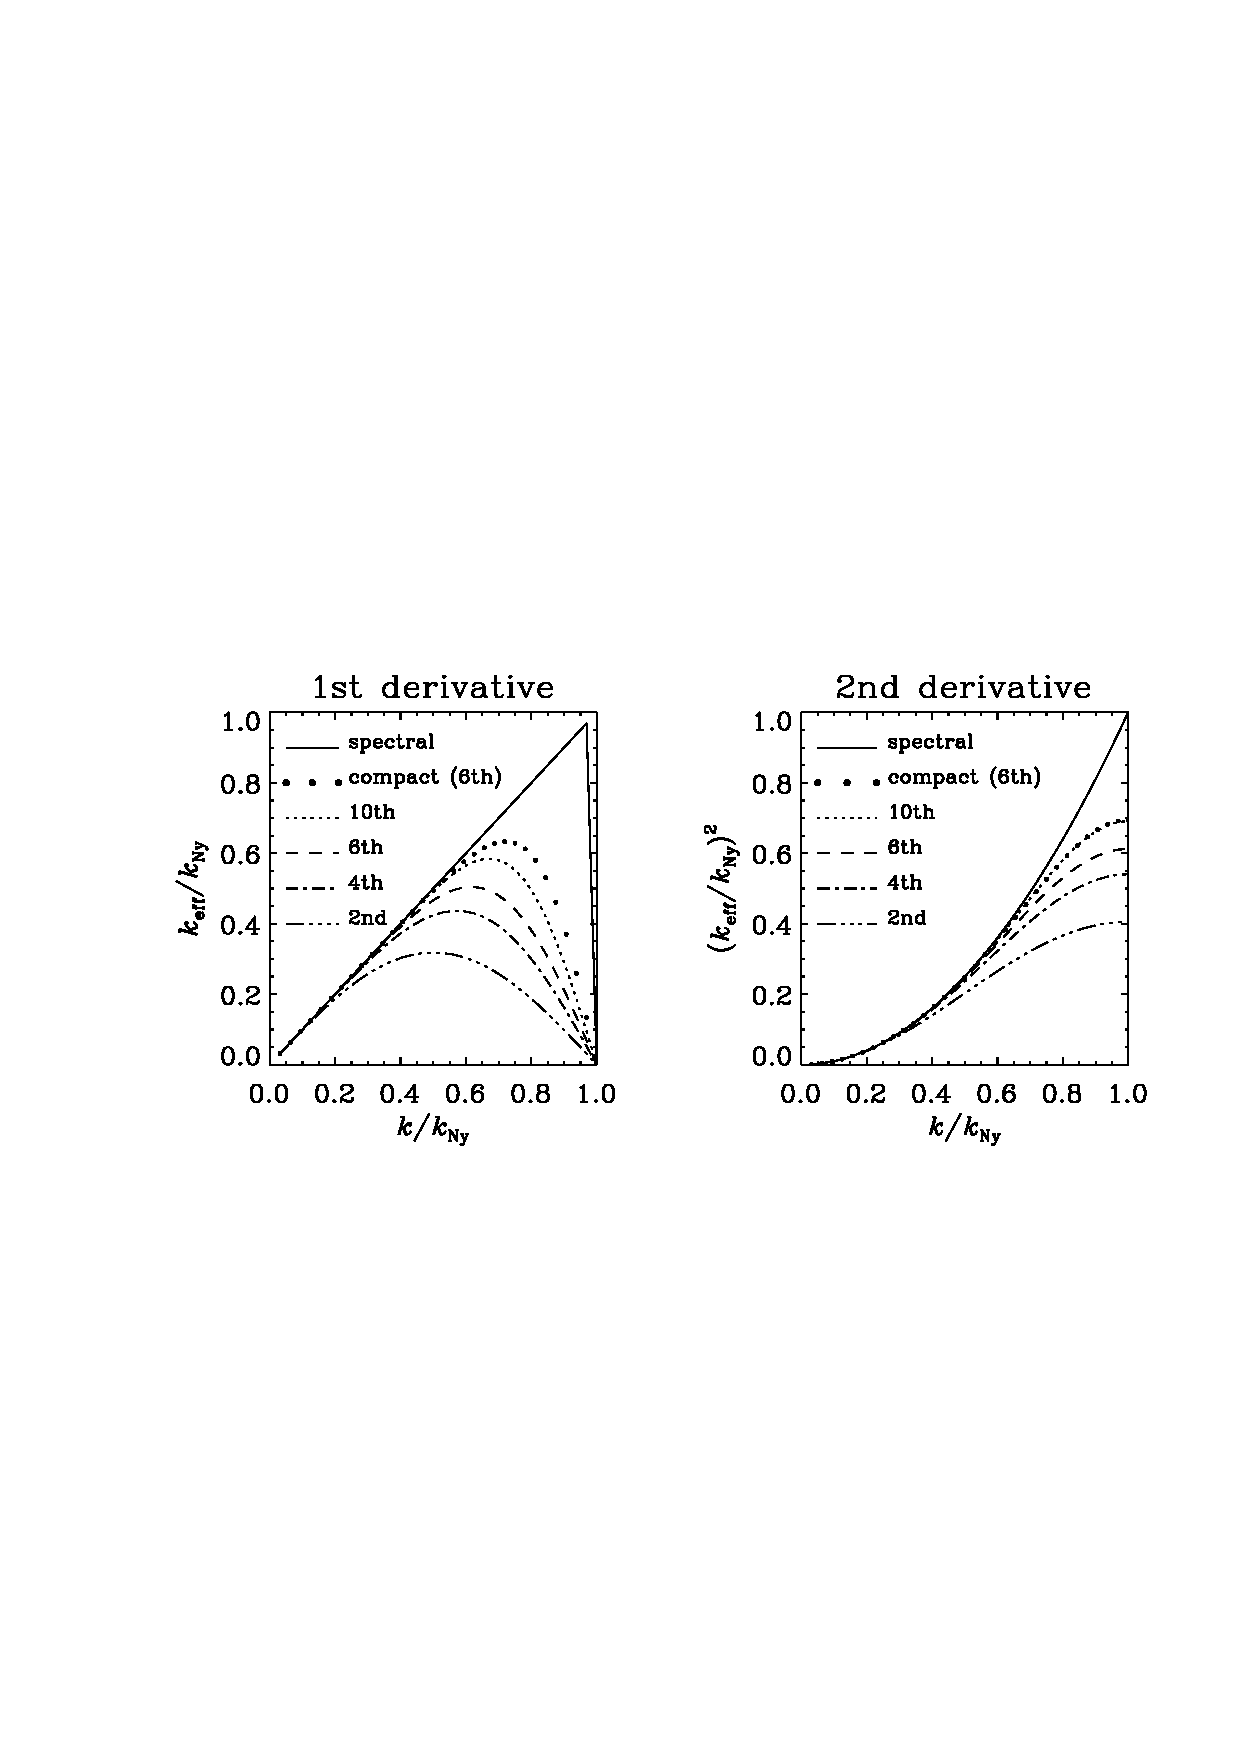
\includegraphics[width=.99\textwidth]
{pkeff}\end{center}\caption[]{
Effective wave numbers for first and second derivatives using different
schemes. Note that for the second derivatives the sixth order compact
scheme is almost equivalent to the tenth order explicit scheme. For the
first derivative the sixth order compact scheme is still superior to the
tenth order explicit scheme.
}\label{Fpkeff}\end{figure}

In the second panel of Fig.~\ref{Fpkeff} we have plotted effective
wavenumbers for second derivatives, which were calculated as
\begin{equation}
(\cos kx)''_{\rm num}=-k_{\rm eff}^2\cos kx.
\end{equation}
Of particular interest is the behavior of the second derivative at the
Nyquist frequency, because that is relevant for damping zig-zag modes.
For a second-order finite difference scheme $k_{\rm eff}^2$ is only 4,
which is less than half the theoretical value of $\pi^2=9.87$. For fourth,
sixth, and tenth order schemes this value is respectively 5.33, 6.04,
6.83. The last value is almost the same as for the 6th order compact
scheme, which is 6.86. Significantly stronger damping at the Nyquist
frequency can be obtained by using hyperviscosity, which Nordlund \&
Galsgaard (1995) treat as a quenching factor that diminishes the value
of the second derivative for wavenumbers that are small compared with
the Nyquist frequency. Accurate high order second derivatives (with no
quenching factors) are important when calculating the current $\Jv$ in
the Lorentz force $\Jv\times\Bv$ from a vector potential $\Av$ using
$-\mu_0\Jv=\nabla^2\Av-\nab\nab\cdot\Av$. This will be important in
the MHD calculations presented below. \index{Hyperviscosity}


\subsection{Upwind derivatives to avoid `wiggles'}
\index{Upwinding}
\label{S-upwind}
\newcommand{\Order}[1]{O\left(#1\right)}

High-order centered-difference convection simulations often show
``wiggles'' (Nyquist zigzag pattern) in $\ln\rho$, which are apparently
caused by a velocity profile where the velocity approaches zero on the
boundary or inside the box.\footnote{%
  A simple one-dimensional test profile would be $u(x) = 1-x^2$ on $x \in
  [-1,1]$, which will accumulate more and more mass near the right
  boundary $x=1$.

  In two- or three-dimensional settings, the presence of stagnation points
  of X-type leads to the same configuration, this time with the
  possibility of a steady state (i.e.~without accumulation of mass).
  Such stagnation points occur e.g.~at the top of an upwelling, or at
  the bottom of a downdraft in convection simulations, where locally
  $u_z \propto z_{\rm X}-z$.
}
This causes the density profile to be squeezed into a boundary layer where
eventually numerical resolution is insufficient and, for centered
differences, a spurious Nyquist signal is generated that almost
instantaneously propagates into much of the whole box.

Even if the stagnation point is on the boundary (and enforced by the
boundary conditions), this behavior is hardly influenced by the boundary
conditions on $\ln\rho$ at all.
A solution, however, is to apply upwinded derivative operators.
The simplest upwind derivative is a finite-difference derivative operator
where the point furthest downwind is excluded from the stencil.
For $u>0$, that means that instead of
\begin{equation}
  f'_0
  = \frac{-f_{-3} + 9 f_{-2} - 45 f_{-1} \qquad
           + 45 f_{1} - 9 f_{2} + f_{3}}
         {60\,\delta x}
    - \frac{\delta x^6\,f^{(7)}}{140}
  = D^{\rm(cent,6)} + \Order{\delta x^6} \; ,
\end{equation}
one takes
\begin{equation}
  f'_0
  = \frac{-2 f_{-3} + 15 f_{-2} - 60 f_{-1} + 20 f_{0} + 30 f_{1} - 3 f_{2}}
         {60\,\delta x}
    + \frac{\delta x^5\,f^{(6)}}{60}
  = D^{\rm(up,5)} + \Order{\delta x^5} \; .
\end{equation}
A fourth-order upwind scheme (excluding two downwind points) would be
\begin{equation}
  f'_0
  = \frac{-f_{-3} + 6 f_{-2} - 18 f_{-1} + 10 f_{0} + 3 f_{1}}
         {12\,\delta x}
    - \frac{\delta x^4\,f^{(5)}}{20}
  = D^{\rm(up,4)} + \Order{\delta x^4} \; .
\end{equation}
The effect of upwinding is mostly to stop the Nyquist perturbations from
spreading away from the boundary or stagnation point.
With the fourth-order formula they actually hardly ever develop.

The difference between central and fifth-order upwind derivative is
\begin{equation}
  [D^{\rm(up,5)} - D^{\rm(cent,6)}] f_0
  = \frac{-f_{-3} + 6 f_{-2} - 15 f_{-1} + 20 f_{0}
          - 15 f_{1} + 6 f_{2} - f_{3}}
         {60\,\delta x}
  = -\frac{\delta x^5}{60} f^{(6)}_{0} \; .
\end{equation}
In other words, 5th-order upwinding can be represented for any sign of $u$
as hyperdiffusion (Dobler et al.\ 2006): \index{Hyperviscosity}
\begin{equation} \label{Eq-upwind-hyperdiff}
  -u f'_{\rm(up,5th)}
  = -u f'_{\rm(centr,6th)}  + \frac{|u|\,\delta x^5}{60} f^{(6)} \; .
\end{equation}
The advantage over adopting constant hyperdiffusion is that in the
upwinding scheme hyperdiffusion is only applied where it is needed
(i.e.~where advection is happening, hence the factor $|u|$).
 \index{Hyperviscosity}

The form (\ref{Eq-upwind-hyperdiff}) also suggests an easy way to get
`stronger' upwinding: Rather than excluding more points in the downwind
direction, we can simply treat the weight of the hyperdiffusion term as a
free parameter $\alpha$:
\begin{equation}
  -u f'_{\rm(up,5th,\alpha)}
  = -u f'_{\rm(centr,6th)}  + \alpha\,|u|\,\delta x^5 f^{(6)} \; .
\end{equation}
If $\alpha$ is large, this may affect the time step, but for
$\alpha=1/60$, the stability requirement for the hyperdiffusive term
should always be weaker than the advective Courant criterion.

\subsection{The bidiagonal scheme for cross-derivatives}
\index{Bidiagonal scheme}
\label{Bidiagonal}

The {\em old} default scheme used for cross-derivatives of type
$\partial^2/(\partial x \partial y)$ used to read as follows:
\begin{verbatim}
      df=fac*( &
                  270.*( f(l1+1:l2+1,m+1,n,k)-f(l1-1:l2-1,m+1,n,k)  &
                        +f(l1-1:l2-1,m-1,n,k)-f(l1+1:l2+1,m-1,n,k)) &
                 - 27.*( f(l1+2:l2+2,m+2,n,k)-f(l1-2:l2-2,m+2,n,k)  &
                        +f(l1-2:l2-2,m-2,n,k)-f(l1+2:l2+2,m-2,n,k)) &
                 +  2.*( f(l1+3:l2+3,m+3,n,k)-f(l1-3:l2-3,m+3,n,k)  &
                        +f(l1-3:l2-3,m-3,n,k)-f(l1+3:l2+3,m-3,n,k)) &
             )
\end{verbatim}
and is ``visualized'' in the left part of Fig.~\ref{Fig-bidiagonal-scheme}.
It is way more efficient than the straight-forward approach of first
taking the $x$ and the $y$ derivative consecutively.
(shown in the right part of Fig.~\ref{Fig-bidiagonal-scheme}).

% ---------------------------------------------------------------------- %
\begin{figure}[h]
  \centering
  \footnotesize

  \begin{tabular}{|c|c|c|c|c|c|c|}
    \hline
    -2 & 0   & 0    & 0 & 0    & 0   & +2 \\
    \hline
    0  & +27 & 0    & 0 & 0    & -27 & 0  \\
    \hline
    0  & 0   & -270 & 0 & +270 & 0   & 0  \\
    \hline
    0  & 0   & 0    & 0 & 0    & 0   & 0  \\
    \hline
    0  & 0   & +270 & 0 & -270 & 0   & 0  \\
    \hline
    0  & -27 & 0    & 0 & 0    & +27 & 0  \\
    \hline
    +2 & 0   & 0    & 0 & 0    & 0   & -2 \\
    \hline
  \end{tabular}\
  \qquad\qquad\
  \begin{tabular}{|c|c|c|c|c|c|c|}
    \hline
    9    & -27  & 135   & 0 & -135  & 27   & -9   \\
    \hline
    -27  & 81   & -405  & 0 & 405   & -81  & 27   \\
    \hline
    135  & -405 & 2025  & 0 & -2025 & 405  & -135 \\
    \hline
    0    & 0    & 0     & 0 & 0     & 0    & 0    \\
    \hline
    -135 & 405  & -2025 & 0 & 2025  & -405 & 135  \\
    \hline
    27   & -81  & 405   & 0 & -405  & 81   & -27  \\
    \hline
    -9   & 27   & -135  & 0 & 135   & -27  & 9    \\
    \hline
  \end{tabular}

  \caption{Weights of bidiagonal scheme (left) and consecutive scheme
    (right) for mixed derivatives $\partial^2/\partial x \partial y$.
    The numbers shown need to be divided by $720\,\delta x\,\delta y$ for
    the bidiagonal and by $3600\,\delta x\,\delta y$ for the consecutive
    scheme.
  }
  \label{Fig-bidiagonal-scheme}
\end{figure}
% ---------------------------------------------------------------------- %

Off-diagonal terms enter not only the diffusion terms through
$\nab\nab\cdot\uv$ and $\nab\nab\cdot\Av$ terms, but also through
the $\Jv=\nab\times\nab\times\Av$ operator.
The general formula is $J_i=A_{j,ij}-A_{i,jj}$, so in 2-D in the
$xy$-plane we have
\begin{eqnarray}
  J_x &=& A_{x,xx}+A_{y,xy}-A_{x,xx}-A_{x,yy}=A_{y,xy}-A_{x,yy} \; , \\
  J_y &=& A_{x,yx}+A_{y,yy}-A_{y,xx}-A_{y,yy}=A_{x,yx}-A_{y,xx}
\end{eqnarray}

\begin{figure}[h]
  \centering
  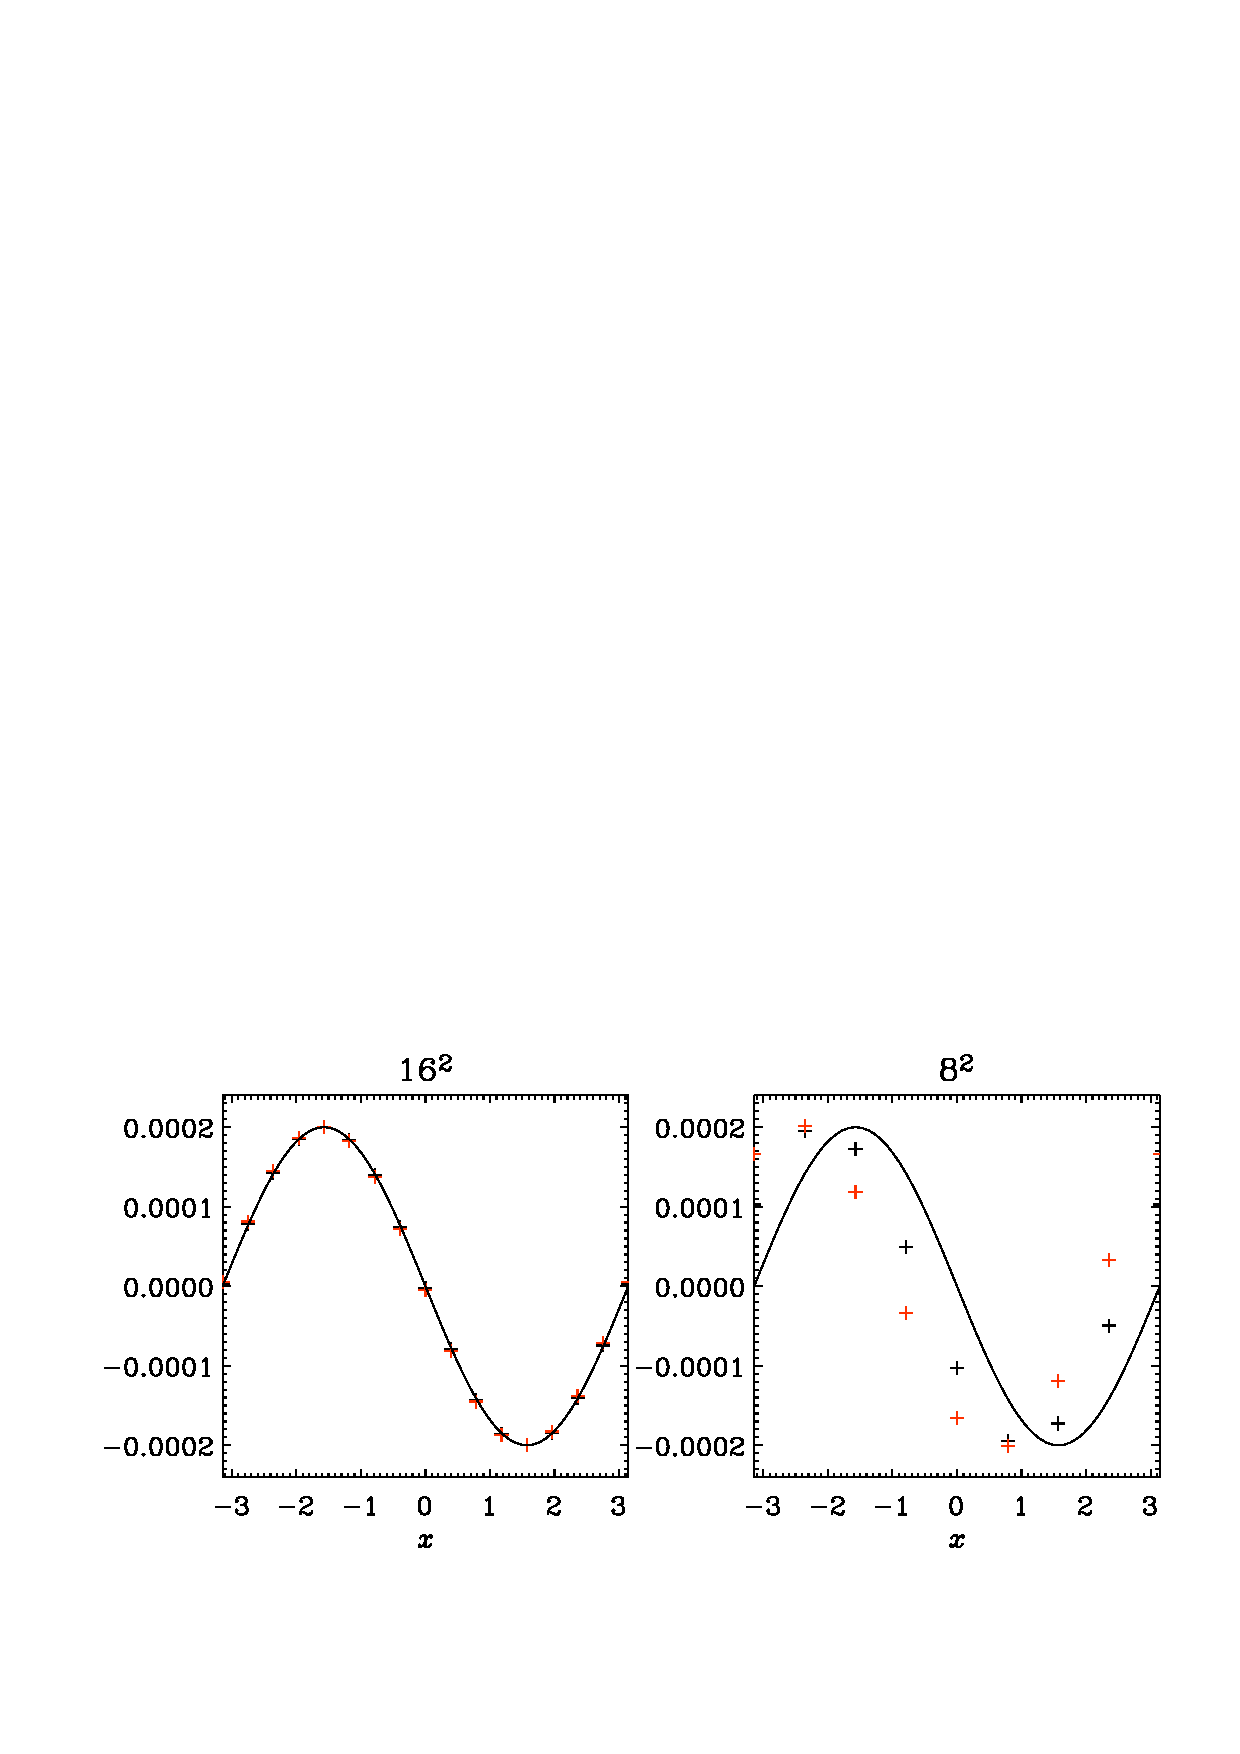
\includegraphics[width=\columnwidth]{pcompbidiagonal}
  \caption{
    Alfv\'en wave for $\Bv_0=(1,2,0)$ and $\kv=(1,2,0)$ after $t=2\pi$.
    The wave travels in the direction of $\kv$.
    Red symbols are for the bidiagonal scheme, black symbols show results
    obtained using the consecutive scheme.
    Already for $16^2$ mesh points there are no clear differences.
    For $8^2$ mesh points both schemes are equally imprecise regarding
    the phase error, but the amplitude error is still quite small
    (but this is mainly a property of the time stepping scheme).
  }
  \label{Fig-pcompbidiagonal}
\end{figure}

Figure \ref{Fig-pcompbidiagonal} shows how the two schemes perform for the
propagation of Alfv\'en waves,

\begin{eqnarray}
  \dot{u}_z &=& J_xB_{0y}-J_yB_{0x} \; , \\
  \dot{A}_x &=& -u_zB_{0y} \; , \\
  \dot{A}_y &=& +u_zB_{0x} \; .
\end{eqnarray}
The initial condition (as implemented in \texttt{subroutine alfven\_xy})
is
\begin{eqnarray}
  u_z &\sim& \cos(k_xx+k_yy-\omega t) \; , \\
  A_x &\sim& +B_{0y}\sin(k_xx+k_yy-\omega t)/\omega \; , \\
  A_y &\sim& -B_{0x}\sin(k_xx+k_yy-\omega t)/\omega \; ,
\end{eqnarray}
where $\omega=\kv\cdot\Bv_0$.
The figure shows that there is no clear advantage of either scheme, so the
code uses the more efficient bidiagonal one.

\subsection{The 2N-scheme for time-stepping}
\index{2N-scheme}
\index{Time step}
\index{Runge-Kutta}
\label{S-2N-scheme}

For time stepping, higher-order schemes are necessary in order to reduce
the amplitude and phase errors of the scheme and, to some extent, to allow
longer time steps.
Usually such schemes require large amounts of memory.
However, we here use the memory-effective $2N$-schemes that require only
two sets of variables to be held in memory.
Such schemes work for
arbitrarily high order, although not all Runge-Kutta schemes can be
written as $2N$-schemes \cite{2Nstorage,SH88}.
Consider the ordinary differential equation (ODE)
\begin{equation}
  \dot{u} = F(u,t) \; ,
\end{equation}
which can also be used as a prototype for a system of ODEs to be solved,
like the ones obtained by spatial discretization of PDEs.
The $2N$-schemes construct an approximation to the solution
\begin{equation}
  u^{(n)} \equiv u(t_n)
\end{equation}
according to the iterative procedure
\begin{eqnarray}
  w_i &=& \alpha_i w_{i-1}+\delta t\,F(u_{i-1},t_{i-1}) \;, \\
  u_i &=& u_{i-1}+\beta_i w_i \;.
\label{iterform0}
\end{eqnarray}
For a three-step scheme we have $i=1,...,3$.
In order to advance the variable $u$ from $u^{(n)}$ at time $t^{(n)}$
to $u^{(n+1)}$ at time $t^{(n+1)}=t^{(n)}+\delta t$ we set in \Eq{iterform0}
\begin{equation}
  u_0=u^{(n)}
  \quad\mbox{and, after the last step,}\quad
  u^{(n+1)}=u_3,
\end{equation}
with $u_1$ and $u_2$ being intermediate steps. In order to be able to
calculate the first step, $i=1$, for which no $w_{i-1}\equiv w_0$ exists,
we have to require $\alpha_1=0$. Thus, we are left with 5 unknowns,
$\alpha_2$, $\alpha_3$, $\beta_1$, $\beta_2$, and $\beta_3$. Three
conditions follow from the fact that the scheme be third order
for linear equations, so we
have to have two more conditions. One possibility is to choose the
fractional times at which the right hand side is evaluated, for
example $(0,1/3,2/3)$ or even $(0,1/2,1)$.
Yet another possibility is to require that
inhomogeneous equations of the form $\dot{u}=t^n$ with $n=1$ and 2 are
solved exactly.
The corresponding coefficients are listed in Table~\ref{T-2N-RK3} and compared
with those given by Williamson \cite{2Nstorage}. In practice all of them
are about equally good when it comes to real applications, although
we found the first one in Table~\ref{T-2N-RK3} (`symmetric') marginally better in some
simple test problems where an analytic solution was known.
In Ref.~\cite{Ref-1} the accuracy of some nonlinear equations is tested.

\begin{table}[htb]
  \centering
  \caption{
    Coefficients for different $2N$-type third-order Runge-Kutta
    schemes.
    The coefficients $c_i$ (which are determined by the $\alpha_i$,
    $\beta_i$) give the time for each substep,
    $t_i = t_0 + c_i \delta t$
    }\label{T-2N-RK3}
  \vspace{12pt}
  \begin{tabular}{l@{\quad}ccc@{\quad}cc@{\quad}ccc}
    \toprule
    scheme            & $c_1$
                            & $c_2$
                                    & $c_3$
                                              & $\alpha_2$
                                                         & $\alpha_3$
                                                                    & $\beta_1$
                                                                            &$\beta_2$
                                                                                    & $\beta_3$\\
    \midrule
    symmetric         & $0$ & $1/3$ & $2/3$   &  $-2/3$  &   $-1$   & $1/3$ &  $1$  & $1/2$ \\
    {}[predictor/corrector]
                      & $0$ & $1/2$ & $1$     &  $-1/4$  &  $-4/3$  & $1/2$ & $2/3$ & $1/2$ \\
    inhomogeneous     & $0$ & $15/32$ & $4/9$ & $-17/32$ & $-32/27$ & $1/4$ & $8/9$ & $3/4$ \\
    Williamson (1980) & $0$ & $4/9$ & $15/32$ &  $-5/9$  &$-153/128$& $1/3$ &$15/16$& $8/15$\\
    \bottomrule
  \end{tabular}
\end{table}

\subsection{Ionization}
\index{Ionization}
\label{S-Ioni}

The specific entropy of each particle species (neutral hydrogen, electrons, protons and neutral helium) may be written as
\begin{equation}
\frac{s_i}{s_0}=x_i\left(\ln\left[\frac{1}{x_{\rm tot}}
\frac{\rho_i}{\rho}\left(\frac{T}{T_0}\right)^{3/2}\right]
+\frac{5}{2}\right)\ ,
\end{equation}
where
\begin{equation}
x_{\rm H}=1-y\ ,\quad x_{\rm e}=x_{\rm p}=y\ ,\quad x_{\rm tot}=1+y+x_{\rm He}
\end{equation}
\begin{equation}
s_0=\frac{k_{\rm B}}{\mu m_{\rm H}}\ ,\quad
T_0=\frac{\chi_{\rm H}}{k_{\rm B}}\ ,
\end{equation}
and
\begin{equation}
\rho_i=\mu m_{\rm H}\left(\frac{m_i\chi_{\rm H}}{2\pi\hbar^2}\right)^{3/2}\ .
\end{equation}
The specific entropy of mixing is
\begin{equation}
\frac{s_{\rm mix}}{s_0}=-\sum_ix_i\ln\frac{x_i}{x_{\rm tot}}\ .
\end{equation}
Summing up everything, we get the total specific entropy
\begin{align}
\frac{s}{s_0}&=\sum_i\frac{s_i}{s_0}+\frac{s_{\rm mix}}{s_0}
=\sum_ix_i\left(\ln\left[\frac{1}{x_i}\frac{\rho_i}{\rho}
\left(\frac{T}{T_0}\right)^{3/2}\right]+\frac{5}{2}\right)\\
&=\sum_ix_i\ln\frac{\rho_i}{x_i}
+x_{\rm tot}\left(\ln\left[\frac{1}{\rho}
\left(\frac{T}{T_0}\right)^{3/2}\right]+\frac{5}{2}\right)\ .
\end{align}
Solving for $T$ gives
\begin{equation}
\frac{3}{2}\ln\frac{T}{T_0}=\frac{s/s_0
+\sum_ix_i\ln x_i/\rho_i}{x_{\rm tot}}
+\ln\rho-\frac{5}{2}\ .
\end{equation}
Using this expression and the constants defined above, we may obtain the
ionization fraction $y$ for given $\ln\rho$ and $s$ by finding the root of
\begin{equation}
F=\ln\left[\frac{\rho_{\rm e}}{\rho}\left(\frac{T}{T_0}\right)^{3/2}
           \frac{1-y}{y^2}\right]-\frac{T_0}{T}\ .
\end{equation}
The derivative with respect to $y$ for Newton-Raphson is
\begin{equation}
\frac{\partial F}{\partial y}
=\left(\frac{3}{2}+\frac{T_0}{T}\right)\frac{\partial\ln T/T_0}{\partial y}
 -\frac{1}{1-y}-\frac{2}{y}\ ,
\end{equation}
where
\begin{equation}
\frac{\partial\ln T/T_0}{\partial y}
=\frac{\frac{2}{3}\left(\ln\rho_{\rm H}/\rho_{\rm p}-F-T_0/T\right)-1}
      {1+y+x_{\rm He}}\ .
\end{equation}
In order to compute the pressure gradient in the momentum equation,
the derivative of $y$ with respect
to $\ln\rho$ and $s$ needs to be known:
\begin{equation}
\frac{\partial\ln P}{\partial\ln\rho}
=\frac{1}{1+y+x_{\rm He}}\frac{\partial y}{\partial\ln\rho}
+\frac{\partial\ln T}{\partial\ln\rho}
+\frac{\partial\ln T}{\partial y}\frac{\partial y}{\partial\ln\rho}+1,
\end{equation}
\begin{equation}
\frac{\partial\ln P}{\partial s}
=\frac{1}{1+y+x_{\rm He}}\frac{\partial y}{\partial s}
+\frac{\partial\ln T}{\partial s}
+\frac{\partial\ln T}{\partial y}\frac{\partial y}{\partial s}.
\end{equation}
Since $F=0$ for all desired solutions $(y,\ln\rho,s)$ we also have
\begin{equation}
dF=\frac{\partial F}{\partial\ln\rho}{\rm d}\ln\rho
   +\frac{\partial F}{\partial s}{\rm d} s
   +\frac{\partial F}{\partial y}{\rm d} y=0\ ,
\end{equation}
and thus
\begin{equation}
\frac{\partial y}{\partial\ln\rho}
=\left(\frac{{\rm d} y}{{\rm d}\ln\rho}\right)_{{\rm d} s=0}
=-\frac{\partial F/\partial\ln\rho}{\partial F/\partial y}
\end{equation}
and
\begin{equation}
\frac{\partial y}{\partial s}
=\left(\frac{{\rm d} y}{{\rm d} s}\right)_{{\rm d}\ln\rho=0}
=-\frac{\partial F/\partial s}{\partial F/\partial y}.
\end{equation}

% --------------------------------------------------------------------- %

\subsection{Radiative transfer}
\index{Radiative transfer}
\label{S-radi-trans}

\subsubsection{Solving the radiative transfer equation}

A formal solution of Eq.~(\ref{radiative-transfer}) is given by
\begin{equation}
  I(\tau) = I(\tau_0) e^{-(\tau-\tau_0)}
            + \int\limits_{\tau_0}^\tau e^{-(\tau-\tau')} S(\tau')\,d\tau' \; .
\end{equation}
Using a generalization of the trapezoidal rule,
\begin{eqnarray}
  \int\limits_{\tau_0}^\tau e^{-(\tau-\tau')} f(\tau')\,d\tau'
  &\approx& \int\limits_{\tau_0}^\tau e^{-(\tau-\tau')}
              \left[ f(\tau_0) + \frac{f(\tau){-}f(\tau_0)}{\tau-\tau_0}\,
              (\tau'-\tau_0)\right] \; d\tau'\\
  &=&       \left[1{-}e^{-(\tau-\tau_0)}\right] f(\tau)
          - \frac{1 - e^{-(\tau-\tau_0)}(1+\tau{-}\tau_0)}{\tau-\tau_0}
            [f(\tau)-f(\tau_0)]
  \; ,
\end{eqnarray}
which is exact for linear functions $S(\tau)$, we discretize this as
\begin{eqnarray}
  I_{k+1} &=& I_k e^{-\delta\tau}
              + (1{-}e^{-\delta\tau}) S_{k+1}
              - \frac{1 - e^{-\delta\tau}(1+\delta\tau)}{\delta\tau}
                (S_{k+1}-S_k) \; , \\
          &=& I_k e^{-\delta\tau}
              + (1{-}e^{-\delta\tau}) S_{k}
              + \frac{e^{-\delta\tau}-1+\delta\tau}{\delta\tau}
                (S_{k+1}-S_k) \; .
\end{eqnarray}
Here the simplest way to calculate $\delta\tau$ is
\begin{equation}
  \delta\tau = \frac{\chi_k{+}\chi_{k+1}}{2} \, \delta x \; ;
\end{equation}
more accurate alternatives are
\begin{equation}
  \delta\tau = \sqrt{\chi_k\chi_{k+1}} \, \delta x
\end{equation}
or
\begin{equation}
  \delta\tau
  = \frac{\chi_{k+1}-\chi_k}{\ln\frac{\chi_{k+1}}{\ln\chi_k}} \, \delta x
\end{equation}


\subsubsection{Angular integration}

% ---------------------------------------------------------------------- %
\begin{table}[htb]
  \renewcommand{\arraystretch}{2.3}
  \centering
  \caption{Sums $\sqrt{4\pi}Y_l^m(\theta_i,\phi_i)$ for special
    sets of directions.
    For all degrees and orders up to $l=8$ not mentioned in this table,
    the sums are $0$.
    The label `Non-h.~f-d.' stands for `non-horizontal face-diagonals',
    i.e.~the eight face diagonals that are not in the horizontal plane.
  }
  \label{Tab-Ylm-sums}
  \footnotesize
  \begin{tabular}{lr@{\qquad}r@{\qquad}rr@{\qquad}rr@{\qquad}rrr}
  \toprule
    Directions   & $Y_0^0$   & $Y_2^0$      & $Y_4^0$          & $Y_4^{\pm4}$             & $Y_6^0$                    & $Y_6^{\pm4}$                & $Y_8^0$                     & $Y_8^{\pm4}$                 & $Y_8^{\pm8}$                  \\
  \midrule
    Coord.       &  $6$      & $0$          &  $\dfrac{21}{2}$ &  $\dfrac{3}{4}\sqrt{70}$ &  $\dfrac{3}{4}\sqrt{13}$   & $-\dfrac{3}{8}\sqrt{182}$   & $\dfrac{99}{32}\sqrt{17}$   & $\dfrac{3}{32}\sqrt{2618}$   & $\dfrac{3}{64}\sqrt{24310}$   \\
    Face diag.   & $12$      & $0$          & $-\dfrac{21}{4}$ & $-\dfrac{3}{8}\sqrt{70}$ & $-\dfrac{39}{16}\sqrt{13}$ &  $\dfrac{39}{32}\sqrt{182}$ & $\dfrac{891}{256}\sqrt{17}$ & $\dfrac{27}{256}\sqrt{2618}$ & $\dfrac{27}{512}\sqrt{24310}$ \\
    Space diag.  &  $8$      & $0$          & $-\dfrac{28}{3}$ & $-\dfrac{2}{3}\sqrt{70}$ & $\dfrac{16}{9}\sqrt{13}$  & $-\dfrac{8}{9}\sqrt{182}$   & $\dfrac{11}{9}\sqrt{17}$    & $\dfrac{1}{27}\sqrt{2618}$   & $\dfrac{1}{54}\sqrt{24310}$   \\
  \midrule
    Non-h.~f-d.  &  $8$      & $2\sqrt{5}$  & $-\dfrac{39}{4}$ &  $\dfrac{3}{8}\sqrt{70}$ & $-\dfrac{19}{16}\sqrt{13}$ & $\dfrac{27}{32}\sqrt{182}$  & $\dfrac{611}{256}\sqrt{17}$ & $\dfrac{51}{256}\sqrt{2618}$ & $\dfrac{3}{512}\sqrt{24310}$  \\
    Coord.
    $x$, $y$     &  $4$      & $-2\sqrt{5}$ & $\dfrac{9}{2}$   &  $\dfrac{4}{3}\sqrt{70}$ & $-\dfrac{5}{4}\sqrt{13}$   & $-\dfrac{3}{8}\sqrt{182}$   & $\dfrac{35}{32}\sqrt{17}$   & $\dfrac{3}{32}\sqrt{2618}$   & $\dfrac{3}{64}\sqrt{24310}$   \\
    Coord. $z$   &  $2$      & $2\sqrt{5}$  & $6$              &  $0$                     & $2\sqrt{13}$               & $0$                         & $2\sqrt{17}$                & $0$                          & $0$                           \\
  \bottomrule
  \end{tabular}
\end{table}
% ---------------------------------------------------------------------- %

For angular integration over the full solid angle, we make the ansatz
\begin{equation}
  \int\limits_{4\pi} f(\theta,\phi)\,\frac{d\omega}{4\pi}
  = \sum_{i=1}^{N} w_i f(\theta_i,\phi_i) + R_N \; .
\end{equation}
Table \ref{Tab-Ylm-sums} shows the sums
$\sqrt{4\pi}Y_l^m(\theta_i,\phi_i)$ over special sets of directions
$(\theta_i,\phi_i)$.
Using these numbers and requiring that angular integration is exact for
$l\le l_{\rm max}$, we find the following weights $w_i$ for different sets
of directions (see also \cite{Abramowitz-Stegun}, \S 25.4.65):

\begin{enumerate}
\item \emph{Axes}

  \begin{tabular}{@{}lr}
    Coordinate axes: & 1/6
  \end{tabular}

  $l_{\rm max} = 3$

\item \emph{Face diagonals}

  \begin{tabular}{@{}lr}
    Face diagonals: & 1/12
  \end{tabular}

  $l_{\rm max} = 3$

\item \emph{Space diagonals}

  \begin{tabular}{@{}lr}
    Space diagonals: & 1/8
  \end{tabular}

  $l_{\rm max} = 3$

\item \emph{Axes + face diagonals}

  \begin{tabular}{@{}lr}
    Coordinate axes: & 1/30 \\
    Face diagonals:  & 1/15 \\
  \end{tabular}

  $l_{\rm max} = 5$

\item \emph{Axes + space diagonals}

  \begin{tabular}{@{}lr}
    Coordinate axes: & 1/15 \\
    Space diagonals: & 3/40 \\
  \end{tabular}

  $l_{\rm max} = 5$

\item \emph{Face + space diagonals}

  \begin{tabular}{@{}lr}
    Face diagonals:  &  2/15 \\
    Space diagonals: & -3/40 \\
  \end{tabular}

  $l_{\rm max} = 5$

\item \emph{Axes, face + space diagonals}

  \begin{tabular}{@{}lr}
    Coordinate axes: & 1/21 \\
    Face diagonals:  & 4/105 \\
    Space diagonals: & 9/280 \\
  \end{tabular}

  $l_{\rm max} = 7$

\item \emph{Axes, non-horizontal face diagonals}

  \begin{tabular}{@{}lr}
    Coordinate axes $x$, $y$: & 1/10 \\
    Coordinate axes $z$:      & 1/30 \\
    Non-hor.~face diagonals:  & 1/15 \\
  \end{tabular}

  $l_{\rm max} = 3$

\item \emph{Axes, non-horizontal face diagonals, space diagonals}

  \begin{tabular}{@{}lr}
    Coordinate axes $x$, $y$: & 12/215 \\
    Coordinate axes $z$:      & 10/129 \\
    Non-hor.~face diagonals:  & -14/645 \\
    Space diagonals:          & 171/1720 \\
  \end{tabular}

  $l_{\rm max} = 5$

\end{enumerate}


% ====================================================================== %

\section{Switchable modules}
  \label{Tab-modules}

%% $Id$
%% This file was automatically generated by Pencil::DocExtractor,
%% so think twice before you modify it.
%%
%% Source files:
%%   hydro.f90
%%   noentropy.f90
%%   nohydro.f90
%%   nopower_spectrum.f90
%%   power_spectrum.f90
%%   timestep.f90
%%   timestep_subcycle.f90

% ---------------------------------------------------------------- %
\begin{longtable}{lp{0.9\textwidth}}
\toprule
  \multicolumn{1}{c}{\emph{Module}} & {\emph{Description}} \\
\midrule
  \var{hydro.f90} & This module takes care of most of the things related to velocity. \\
  \var{}          & Pressure, for example, is added in the energy (entropy) module. \\
\midrule
  \var{noentropy.f90} & Calculates pressure gradient term for \\
  \var{}          & polytropic equation of state $p=\text{const}\rho^{\Gamma}$. \\
\midrule
  \var{nohydro.f90} & no variable $\uv$: useful for kinematic dynamo runs. \\
\midrule
  \var{nopower_spectrum.f90} & reads in full snapshot and calculates power spetrum of u \\
\midrule
  \var{power_spectrum.f90} & reads in full snapshot and calculates power spetrum of u \\
\midrule
  \var{timestep.f90} & Runge-Kutta time advance, accurate to order itorder. \\
  \var{}          & At the moment, itorder can be 1, 2, or 3. \\
\midrule
  \var{timestep_subcycle.f90} & This is a highly specified timestep module currently only working \\
  \var{}          & together with the special module coronae.f90. \\
%
\bottomrule
\end{longtable}



% %(AB: this is no longer a table, so I treat it as section)
% %(AB: but acroread somehow still doesn't bring me to the right place)

% The table below lists the available physics and technical
% modules
% [Note: this is most likely very outdated and should probably be automated]

% % ---------------------------------------------------------------------- %
% %\begin{table}
% \begin{center}
%   \begin{small}
% %  \caption{%
% %    Switchable modules as of September 2002.
% %  }
% % \label{Tab-modules}
% %  \begin{tabular}{lp{0.6\textwidth}}
%   \begin{longtable}{lp{0.6\textwidth}}
%     \toprule
%     \file{hydro.f90}      & Hydrodynamics: add variable $\uv$ with equation of
%                             motion; \\
%     \file{nohydro.f90}    & no variable $\uv$: useful for kinematic dynamo
%                             runs. \\
%     \midrule
%     \file{density.f90}    & Add variable $\ln\rho$ with continuity
%                             equation; \\
%     \file{nodensity.f90}  & no variable $\ln\rho$: useful for Burgers'
%                             equation. \\
%     \midrule
%     \file{entropy.f90}    & Add variable $s$ with entropy equation (energy
%                             equation); \\
%     \file{noentropy.f90}  & no variable $s$: isothermal hydrodynamics. \\
%     \midrule
%     \file{magnetic.f90}   & Add variable $\Av$ (magnetic vector potential) with
%                             induction equation; \\
%     \file{nomagnetic.f90} & no variable $\Av$: nonmagnetic hydrodynamics. \\
%     \midrule
%     \file{pscalar.f90}    & Add variable $\ln c$ (concentration) with
%                             advection-diffusion equation for transport of a
%                             passive scalar; \\
%     \file{nopscalar.f90}  & no passive scalar, no variable $\ln c$. \\
%     \midrule
%     \file{radiation_ray.f90} & Radiation transfer along rays.\\
%     \file{noradiation.f90}& No radiative transfer. \\
%     \midrule
%     \file{viscosity.f90} & Constant dynamic or kinematic fluid viscosity. \\
%     \file{noviscosity.f90} & No constant fluid viscosity.\\
%     \midrule
%     \file{shock.f90} & Variable shock
%                             viscosity (conserves energy) based upon
%                             local strength of a shock.
%                             The shock profile is calculated from the
%                             velocity field.
%                             \emph{Still experimental and not fully tested. } \\
%     \file{noshock.f90} & No shock viscosity.\\
%     \midrule
%     \file{forcing.f90}    & Add a forcing function to rhs of equation of motion
%                             (typically helical forcing) for forced turbulence
%                             calculations; \\
%     \file{noforcing.f90}  & no forcing. \\
%     \midrule
%     \file{shear.f90}      & Shearing-box boundary conditions; \\
%     \file{noshear.f90}    & no shearing box. \\
%     \midrule
%     \file{gravity_simple.f90}  & Constant x, y or z gravity in equation of motion; \\
%     \file{grav_r.f90}     & radially symmetric gravity; \\
%     \file{nogravity.f90}     & no gravity. \\
%     \midrule
%     \file{fft.f}          & Singleton (1968) FFT routine: needed for magnetic
%                             potential-field boundary condition; \\
%     \file{nofft.f90}      & no FFT: no need to bother about compiler warnings if
%                             you don't need this boundary condition. \\
%     \midrule
%     \file{io_dist.f90}    & Distributed input/output: each processor writes to
%                             its own directory. \\
%     \file{io_mpio.f90}    & Parallel input/output through \name{MPI-IO}.
%                             \emph{Still experimental}. \\
%     \midrule
%     \file{mpicomm.f90}    & Use \name{MPI} for communication on multiprocessor
%                             machines; \\
%     \file{nompicomm.f90}  & no parallelization: convenient for testing and
%                             smaller production runs on desktop or notebook
%                             computers. \\
%     \midrule
%     \file{debug_c.c}      & Use I/O routines that allow to write auxiliary
%                             variables to a file (nontrivial in a {\sc Pencil Code});
%                             requires C compiler to be set up correctly and maybe
%                             requires appropriate compiler flags
%                             (\code{-DFUNDERSCORE}) for correctly interfacing C
%                             with Fortran (and may still not work in some
%                             cases); \\
%     \file{nodebug.f90}    & don't use these debugging routines, avoiding any
%                             C-Fortran interoperability problems. \\
%     \bottomrule
%   \end{longtable}
% %  \end{tabular}
%   \end{small}
% \end{center}
% %\end{table}
% % ---------------------------------------------------------------------- %



% % ====================================================================== %

\section{Startup and run-time parameters}
\label{S-all-parameters}

\subsection[Startup parameters for \File{start.in}]%
{List of startup parameters for \file{start.in}}
\label{S-all-init-params}

The following table lists all (at the time of writing, September 2002)
namelists used in \file{start.in}, with the corresponding parameters
and their default values (in square brackets).
Any variable referred to as a \dfn{flag} can be set to any nonzero value
to switch the corresponding feature on.
Not all parameters are used for a given scenario.
This list is not necessarily up to date; also, in many cases it can only
give an idea of the corresponding initial state; to get more insight and
the latest set of parameters, you need to look at the code.

The value $\varepsilon$ corresponds to 5 times the smallest number larger
than zero.
For single precision, this is typically about
$\varepsilon \approx 5\times1.2{\times}10^{-7} = 6{\times}10^{-7}$; for
double precision, $\varepsilon\approx10^{-15}$.

% ---------------------------------------------------------------------- %
\begin{longtable}{lp{0.6\textwidth}}
%\begin{tabular}{lp{0.6\textwidth}}
\toprule
  \multicolumn{1}{c}{\emph{Variable [default value]}}
               & \multicolumn{1}{c}{\emph{Meaning}} \\
\midrule
  \multicolumn{2}{c}{Namelist \name{init_pars}}\\
\midrule
  \var{cvsid} [\code{''}]
               & the \name{svn} identification string, which allows you to
                 keep track of the version of \file{start.in}.\\
  \var{ip} [$14$]
               & (anti-)verbosity level: \code{ip=1} produces lots of
                 diagnostic output, \code{ip=14} virtually none. \\
  \var{xyz0} [$(-\pi,-\pi,-\pi)$],\\
  \var{Lxyz} [$(2\pi,2\pi,2\pi)$],\\
  \var{lperi} [(\code{T},\code{T},\code{T})]
               & determine the geometry of the box. All three are vectors
                 of the form ($x$-comp., $y$-comp., $z$-comp.); \var{xyz0}
                 describes the left (lower) corner of the box, \var{Lxyz}
                 the box size.
                 \var{lperi} specifies whether a direction is considered
                 periodic (in which case the last point is omitted) or not.
                 In all cases, three ghost zones will be added. \\
  \var{lprocz_slowest} [\code{T}]
               & if set to \code{F}, the ordering of processor numbers is
                 changed, so the $z$ processors are now in the inner loop.
                 Since \var{nprocy}=4 is optimal (see Sect.~\ref{Bandwidth}),
                 you may want to put \var{lprocz_slowest}=T when
                 \code{nygrid}$>$\code{nzgrid}.\\
  \var{lwrite_ic} [\code{F}]
               & if set \code{T}, the initial data are written into the
                 file \file{VAR0}. This is generally useful, but doing this
                 all the time uses up plenty of disk space.\\
  \var{lnowrite} [\code{F}]
               & if set \code{T}, all initialization files are written,
                 including the param.nml file,
                 except \file{var.dat}. This option allows you to use old
                 file{var.dat} files, but updates all other initialization
                 files. This could be useful after having changed the code
                 and, in particular, when the \file{var.dat} files will be
                 overwritten by \file{remesh.csh}.\\
  \var{lwrite_aux} [\code{F}]
               & if set \code{T}, auxiliary variables (those calculated at
                 each step, but not evolved mathematically) to
                 \file{var.dat} after the evolved quantities. \\
  \var{lwrite_2d} [\code{F}]
               & if set \code{T}, only 2D-snapshots are written into VAR
                 files in the case of 2D-runs with $nygrid=1$ or
                 $nzgrid=1$.\\
  \var{lread_oldsnap} [\code{F}]
               & if set \code{T}, the old snapshot will be read in before
                 producing (overwriting) initial conditions. For example, if
                 you just want to add a perturbation to the magnetic field,
                 you'd give no initial condition for density and velocity
                 (so you keep the data from a hopefully relaxed run),
                 and just add whatever you need for the magnetic field.
                 In this connection you may want to \cmd{touch NOERASE},
                 so as not to erase the previous data.\\
  \var{lread_oldsnap_nomag} [\code{F}]
               & if set \code{T}, the old snapshot from a non-magnetic run
                 will be read in before producing (overwriting) initial
                 conditions. This allows one to let a hydrodynamic
                 run relax before adding a magnetic field. However,
                 for this to work one has to modify {\it manually}
                 \file{data/param.nml} by adding an entry for
                 \var{MAGNETIC_INIT_PARS} or \var{PSCALAR_INIT_PARS}.
                 In addition, for \code{idl} to read correctly after the
                 first restarted run, you must adjust the value of \var{mvar}
                 in \file{data/dim.dat} \\
  \var{lread_oldsnap_nopscalar} [\code{F}]
               & if set \code{T}, the old snapshot from a run without
                 passive scalar will be read in before producing
                 (overwriting) initial conditions. This allows one to
                 let a hydrodynamic run relax before adding a passive
                 scalar.\\
  \var{lshift_origin} [\code{F,F,F}]
               & if set \code{T} for any or some of the three directions,
                 the mesh is shifted by 1/2 meshpoint in that or those
                 directions so that the mesh goes through the origin.\\
  \var{unit_system} [\code{'cgs'}]
               & you can set this character string to \index{SI units}
                 \code{'SI'}, which means that you can give \index{Units}
                 physical dimensions in \index{SI units} SI units.
                 The default is \index{cgs units} cgs units.\\
  \var{unit_length} [\code{1}]
               & allows you to set the unit length. Suppose you want
                 the unit length to be $1\,{\rm kpc}$, then you would
                 say \code{unit_length='3e21'}. (Of course, politically
                 correct would be to say \code{unit_system='SI'} in
                 which case you say \code{unit_length='3e19'}.)\\
  \var{unit_velocity} [\code{1}]
               & Example: if you want km/s you say \code{unit_length='1e5'}.\\
  \var{unit_density} [\code{1}]
               & Example: if you want your unit density to be
                 $10^{-24}\,{\rm g}/{\rm cm}^3$ you say
                 \code{unit_density='1e-24'}.\\
  \var{unit_temperature} [\code{1}]
               & Example: \code{unit_temperature='1e6'} if you want
                 mega-Kelvin.\\
  \var{random_gen} [\code{system}]
               & \label{random-gen-init}
                 choose random number generator;
                 currently valid choices are
                 \begin{description}
                 \item[\code{'system'}] (your compiler's generator),
                 \item[\code{'min_std'}] (the `minimal standard' generator
                   \code{ran0()} from `Numerical Recipes'),
                 \item[\code{'nr_f90'}] (the Parker-Miller-Marsaglia
                   generator \code{ran()} from `Numerical Recipes for
                   F90').
                 \end{description} \\
  \var{bcx} [(\code{'p'}, \code{'p'}, \ldots)], \\
  \var{bcy} [(\code{'p'}, \code{'p'}, \ldots)], \\
  \var{bcz} [(\code{'p'}, \code{'p'}, \ldots)]
               & boundary conditions. See Sect.~\ref{boundconds} for a
                 discussion of where and how to set these. \\
  \var{pretend_lnTT} [\code{F}]
                & \index{pretend_lnTT}
                selects $\ln T$ as fundamental thermodynamic variable
                in the entropy module \\
                 \\
%
\midrule
  \multicolumn{2}{c}{Namelist \name{hydro_init_pars}} \\
\midrule
  \var{inituu} [\code{'zero'}]
               & initialization of velocity. Currently valid choices are
                 \begin{description}
                 \item[\code{`zero'}] ($\uv=0$ ),
                 \item[\code{`gaussian-noise'}] (random,
                   normally-distributed $u_x$,$u_z$),
                 \item[\code{`gaussian-noise-x'}] (random,
                   normally-distributed $u_x$),
                 \item[\code{`sound-wave'}] (sound wave in $x$ direction),
                 \item[\code{`shock-tube'}] (polytropic standing shock),
                 \item[\code{`bullets'}] (blob-like velocity perturbations),
                 \item[\code{`Alfven-circ-x'}] (circularly polarized
                   Alfven wave in x direction),
                 \item[\code{`const-ux'}] (constant x-velocity),
                 \item[\code{`const-uy'}] (constant y-velocity),
                 \item[\code{`tang-discont-z'}] (tangential discontinuity:
                   velocity is directed along $x$, jump is at $z=0$),
                 \item[\code{`Fourier-trunc'}] (truncated Fourier series),
                 \item[\code{`up-down'}] (flow upward in one spot,
                   downward in another; not solenoidal).
                 \end{description}
                 \\
  \var{ampluu} [$0.$]
               & amplitude for some types of initial velocities. \\
  \var{widthuu} [$0.1$]
               & width for some types of initial velocities. \\
  \var{urand} [$0.$]
               & additional random perturbation of $\uv$. If
                 \verb|urand>0|, the perturbation is additive,
                 $u_i \mapsto u_i + u_{\rm rand}{\cal U}_{[0.5,0.5]}$;
                 if \verb|urand<0|, it is multiplicative,
                 $u_i \mapsto u_i \times u_{\rm rand}{\cal U}_{[0.5,0.5]}$;
                 in both cases, ${\cal U}_{[0.5,0.5]}$ is a uniformly
                 distributed random variable on the interval $[-0.5,0.5]$.\\
  \var{uu_left} [$0.$], \\
  \var{uu_right} [$0.$]
               & needed for \code{inituu='shock-tube'}.\\
%
\midrule
  \multicolumn{2}{c}{Namelist \name{density_init_pars}} \\
\midrule
  \var{initlnrho} [\code{'zero'}]
               & initialization of density. Currently valid choices are
                 \begin{description}
                 \item[\code{`zero'}] ($\ln\rho=0$),
                 \item[\code{`isothermal'}] (isothermal stratification),
                 \item[\code{`polytropic\_simple'}] (polytropic stratification),
                 \item[\code{`hydrostatic-z-2'}] (hydrostatic vertical
                   stratification for isentropic atmosphere),
                 \item[\code{`xjump'}] (density jump in $x$ of width
                   \var{widthlnrho}),
                 \item[\code{`rho-jump-z'}] (density jump in $z$ of width
                   \var{widthlnrho}),
                 \item[\code{`piecew-poly'}] (piecewise polytropic vertical
                   stratification for solar convection),
                 \item[\code{`polytropic'}] (polytropic vertical
                   stratification),
                 \item[\code{`sound-wave'}] (sound wave),
                 \item[\code{`shock-tube'}] (polytropic standing shock),
                 \item[\code{`gaussian-noise'}] (Gaussian-distributed,
                   uncorrelated noise),
                 \item[\code{`gaussian-noise'}] (Gaussian-distributed,
                   uncorrelated noise in $x$, but uniform in $y$ and $z$),
                 \item[\code{`hydrostatic-r'}] (hydrostatic radial density
                   stratification for isentropic or isothermal sphere),
                 \item[\code{`sin-xy'}] (sine profile in $x$ and $y$),
                 \item[\code{`sin-xy-rho'}] (sine profile in $x$ and $y$, but
                   in $\rho$, not $\ln\rho$),
                 \item[\code{`linear'}] (linear profile in $\kv\cdot\xv$),
                 \item[\code{`planet'}] (planet solution; see \S\ref{S-planet}).
                 \end{description}
                 \\
  \var{gamma} [$5./3$]
               & adiabatic index $\gamma=c_p/c_v$. \\
  \var{cs0} [$1.$]
               & can be used to set the dimension of velocity;
                 larger values can be used to decrease stratification \\
  \var{rho0} [$1.$]
               & \label{cs0-rho0-init}%
                 reference values of sound speed and density,
                 i.\,e.~values at height \var{zref}. \\
  \var{ampllnrho} [$0.$], \\
  \var{widthlnrho} [$0.1$]
               & amplitude and width for some types of initial densities. \\
  \var{rho_left} [$1.$], \\
  \var{rho_right} [$1.$]
               & needed for \code{initlnrho='shock-tube'}. \\
  \var{cs2bot} [$1.$], \\
  \var{cs2top} [$1.$]
               & sound speed at bottom and top. Needed for some types of
                 stratification. \\
%
\midrule
  \multicolumn{2}{c}{Namelist \name{grav_init_pars}} \\
\midrule
  \var{zref} [$0.$]
               & \label{zref-init}%
                 reference height where in the initial stratification
                 $c_{\rm s}^2=c_{\rm s0}^2$ and $\ln\rho=\ln\rho_0$.\\
  \var{gravz} [$-1.$]
               & vertical gravity component $g_z$.\\
  \var{grav_profile} \\{}
    [\code{'const'}]
               & constant gravity $g_z = \texttt{gravz}$
                 (\code{grav_profile='const'}) gravity
                 or linear profile $g_z = \texttt{gravz}\cdot z$
                 (\code{grav_profile='linear'}, for accretion discs and
                 similar). \\
  \var{z1} [$0.$], \\
  \var{z2} [$1.$]
               & specific to the solar convection case
                 \code{initlnrho='piecew-poly'}.
                 The stable layer is $z_0 < z < z_1$, the unstable layer
                 $z_1 < z < z_2$, and the top (isothermal) layer is
                 $z_2 < z < z_{\rm top}$. \\
  \var{nu_epicycle} [$1.$]
               & vertical epicyclic frequency; for accretion
                 discs it should be equal to Omega, but not for
                 galactic discs; see Eq.~(\ref{disc-gravz-init}) in
                 Sect.~\ref{VerticalStratification}.\\
  \var{grav_amp} [$0.$], \var{grav_tilt} [$0.$]
               & specific to the tilted gravity case (amplitude and angle
                 wrt the vertical direction).\\
%
\midrule
  \multicolumn{2}{c}{Namelist \name{entropy_init_pars}} \\
\midrule
  \var{initss} [\code{'nothing'}]
               & initialization of entropy. Currently valid choices are
                 \begin{description}
                 \item[\code{`nothing'}] (leaves the initialization done
                   in the density module unchanged),
                 \item[\code{`zero'}] (put $s=0$ explicitly; this may
                   overwrite the initialization done in the density module),
                 \item[\code{`isothermal'}] (isothermal stratification,
                   $T=\const$),
                 \item[\code{`isobaric'}] (isobaric, $p=\const$),
                 \item[\code{`isentropic'}] (isentropic with superimposed
                   hot [or cool] bubble),
                 \item[\code{`linprof'}] (linear entropy profile in $z$),
                 \item[\code{`piecew-poly'}] (piecewise polytropic
                   stratification for convection),
                 \item[\code{`polytropic'}] (polytropic stratification,
                   polytropic exponent is \var{mpoly0}),
                 \item[\code{`blob'}] (puts a gaussian blob in entropy for
                   buoyancy experiments; see Ref.~\cite{BH01} for details)
                 \item[\code{`xjump'}] (jump in $x$ direction),
                 \item[\code{`hor-tube'}] (horizontal flux tube in entropy,
                   oriented in the $y$-direction).
                 \end{description}
                 \\
  \var{pertss} [\code{'zero'}]
               & additional perturbation to entropy. Currently valid
                 choices are
                 \begin{description}
                 \item[\code{'zero'}] (no perturbation)
                 \item[\code{'hexagonal'}] (hexagonal perturbation for
                   convection).
                 \end{description}
                 \\
  \var{ampl_ss} [$0.$], \\
  \var{widthss} [$2\varepsilon$]
               & amplitude and width for some types of initial entropy. \\
  \var{grads0} [$0.$]
               & initial entropy gradient for \code{initss=linprof}. \\
  \var{radius_ss} [$0.1$]
               & radius of bubble for \code{initss=isentropic}. \\
  \var{mpoly0} [$1.5$], \\
  \var{mpoly1} [$1.5$], \\
  \var{mpoly2} [$1.5$]
               & \label{mpoly012-init}%
                 specific to the solar convection case
                 \code{initss=piecew-poly}:
                 polytropic indices of unstable (\var{mpoly0}), stable
                 (\var{mpoly1}) and top layer (\var{mpoly2}).
                 If the flag \var{isothtop} is set, the
                 top layer is initialized to be isothermal, otherwise
                 thermal (plus hydrostatic) equilibrium is assumed for all
                 three layers, which results in a piecewise polytropic
                 stratification. \\
  \var{isothtop} [$0$]
               & flag for isothermal top layer for \code{initss=piecew-poly}. \\
  \var{khor_ss} [$1.$]
               & horizontal wave number for \code{pertss=hexagonal} \\
%
\midrule
  \multicolumn{2}{c}{Namelist \name{magnetic_init_pars}} \\
\midrule
  \var{initaa} [\code{'zero'}]
               & initialization of magnetic field (vector potential).
                 Currently valid choices are
                 \begin{description}
                 \item[\code{`Alfven-x'}] (Alfv\'en wave traveling in the
                   $x$-direction; this also sets the velocity),
                 \item[\code{`Alfven-z'}] (Alfv\'en wave traveling in the
                   $z$-direction; this also sets the velocity),
                 \item[\code{`Alfvenz-rot'}] (same as \code{`Alfven-z'}, but
                   with rotation),
                 \item[\code{`Alfven-circ-x'}] (circularly polarized
                   Alfven wave in x direction),
                 \item[\code{`Beltrami-x'}] ($x$-dependent Beltrami wave),
                 \item[\code{`Beltrami-y'}] ($y$-dependent Beltrami wave),
                 \item[\code{`Beltrami-z'}] ($z$-dependent Beltrami wave),
                 \item[\code{`Bz(x)'}] ($B_z\propto\cos(k x)$),
                 \item[\code{`crazy'}] (for testing purposes).
                 \item[\code{`diffrot'}] ([needs to be documented]),
                 \item[\code{`fluxrings'}] (two interlocked magnetic fluxrings;
                   see \S~\ref{fluxrings}),
                 \item[\code{`gaussian-noise'}] (white noise),
                 \item[\code{`halfcos-Bx'}] ([needs to be documented]),
                 \item[\code{`hor-tube'}] (horizontal flux tube in $\Bv$,
                   oriented in the $y$-direction).
                 \item[\code{`hor-fluxlayer'}] (horizontal flux layer),
                 \item[\code{`mag-support'}] ([needs to be documented]),
                 \item[\code{`mode'}] ([needs to be documented]),
                 \item[\code{`modeb'}] ([needs to be documented]),
                 \item[\code{`propto-ux'}] ([needs to be documented]),
                 \item[\code{`propto-uy'}] ([needs to be documented]),
                 \item[\code{`propto-uz'}] ([needs to be documented]),
                 \item[\code{`sinxsinz'}] ($\sin x \sin z$),
                 \item[\code{`uniform-Bx'}] (uniform field in $x$ direction),
                 \item[\code{`uniform-By'}] (uniform field in $y$ direction),
                 \item[\code{`uniform-Bz'}] (uniform field in $z$ direction),
                 \item[\code{`zero'}] (zero field),
                 \end{description}
                 \\
  \var{initaa2} [\code{'zero'}]
               & additional perturbation of magnetic field.
                 Currently valid choices are
                 \begin{description}
                 \item[\code{`zero'}] (zero perturbation),
                 \item[\code{`Beltrami-x'}] ($x$-dependent Beltrami wave),
                 \item[\code{`Beltrami-y'}] ($y$-dependent Beltrami wave),
                 \item[\code{`Beltrami-z'}] ($z$-dependent Beltrami wave).
                 \end{description}
                 \\
  \var{amplaa} [$0.$]
               & amplitude for some types of initial magnetic fields. \\
  \var{amplaa2} [$0.$]
               & amplitude for some types of magnetic field perturbation. \\
  \var[fring1,fring2]{fring\{1,2\}} [$0.$], \\
  \var[Iring1,Iring2]{Iring\{1,2\}} [$0.$], \\
  \var[Rring1,Rring2]{Rring\{1,2\}} [$1.$], \\
  \var[wr1,wr2]{wr\{1,2\}} [$0.3$]
               & flux, current, outer and inner radius of flux ring 1/2;
                 see Sect.~\ref{fluxrings}. \\
  \var{radius} [$0.1$]
               & used by some initial fields. \\
  \var{epsilonaa} [$10^{-2}$]
               & used by some initial fields. \\
  \var{widthaa} [$0.5$]
               & used by some initial fields. \\
  \var{z0aa} [$0.$]
               & used by some initial fields. \\
  \var{kx_aa} [$1.$], \\
  \var{ky_aa} [$1.$], \\
  \var{kz_aa} [$1.$]
               & wavenumbers used by some initial fields. \\
  \var{lpress_equil} [F]
               & flag for pressure equilibrium (can be used in connection
                 with all initial fields) \\
%
\midrule
  \multicolumn{2}{c}{Namelist \name{pscalar_init_pars}} \\
\midrule
  \var{initlncc} [\code{'zero'}]
               & initialization of passive scalar
                 (concentration per unit mass, $c$).
                 Currently valid choices (for $\ln c$) are
                 \begin{description}
                 \item[\code{`zero'}] ($\ln c=0.$),
                 \item[\code{`gaussian-noise'}] (white noise),
                 \item[\code{`wave-x'}] (wave in $x$ direction),
                 \item[\code{`wave-y'}] (wave in $y$ direction),
                 \item[\code{`wave-z'}] (wave in $z$ direction),
                 \item[\code{`tang-discont-z'}] (Kelvin-Helmholtz instability),
                 \item[\code{`hor-tube'}] (horizontal tube in concentration;
                  used as a marker for magnetic flux tubes).
                 \end{description}
                 \\
  \var{initlncc2} [\code{'zero'}]
               & additional perturbation of passive scalar concentration $c$.
                 Currently valid choices are
                 \begin{description}
                 \item[\code{`zero'}] ($\delta\ln c=0.$),
                 \item[\code{`wave-x'}] (add $x$-directed wave to $\ln c$).
                 \end{description}
                 \\
\var{ampllncc} [$0.1$]
               & amplitude for some types of initial concentration. \\
  \var{ampllncc2} [$0.$]
               & amplitude for some types of concentration perturbation. \\
  \var{kx_lncc} [$1.$], \\
  \var{ky_lncc} [$1.$], \\
  \var{kz_lncc} [$1.$]
               & wave numbers for some types of initial concentration. \\
%
\midrule
  \multicolumn{2}{c}{Namelist \name{shear_init_pars}} \\
\midrule
  \var{qshear} [$0.$]
               & \label{qshear-init}%
                 degree of shear for shearing-box simulations (the
                 shearing-periodic boundaries are the $x$-boundaries and
                 are sheared in the $y$-direction). The shear velocity
                 is ${\bf U}=-q\varOmega x\,{\hat{\bf y}}$. \\
\bottomrule
%\end{tabular}
\end{longtable}
% ---------------------------------------------------------------------- %

\subsection[Runtime parameters for \File{run.in}]%
{List of runtime parameters for \file{run.in}}
\label{S-all-run-params}

The following table lists all (at the time of writing, September 2002)
namelists used in file \file{run.in}, with the corresponding
parameters and their default values (in square brackets).
Default values marked as [start] are taken from \file{start.in}.
Any variable referred to as a \dfn{flag} can be set to any nonzero value
to switch the corresponding feature on.
Not all parameters are used for a given scenario.
This list is not necessarily up to date; also, in many cases it can only
give an idea of the corresponding setup; to get more insight and
the latest set of parameters, you need to look at the code.


% ---------------------------------------------------------------------- %
\begin{longtable}{lp{0.6\textwidth}}
%\begin{tabular}{lp{0.6\textwidth}}
\toprule
  \multicolumn{1}{c}{\emph{Variable [default value]}}
               & \multicolumn{1}{c}{\emph{Meaning}} \\
\midrule
  \multicolumn{2}{c}{Namelist \name{run_pars}}\\
\midrule
  \var{cvsid} [\code{''}]
               & \name{svn} identification string, which allows you to
                 keep track of the version of \file{run.in}. \\
  \var{ip} [$14$]
               & (anti-)verbosity level: \code{ip=1} produces lots of
                 additional diagnostic output, \code{ip=14} virtually none. \\
  \var{nt} [$0$]
               & number of time steps to run. This number can be increased
                 or decreased during the run by \cmd{touch RELOAD}.\\
  \var{it1} [$10$]
               & write diagnostic output every \var{it1} time steps
                 (see Sect.~\ref{diagnostic-IO}). \\
  \var{it1d} [$it1$]
               & write averages every \var{it1d} time steps
                 (see Sect.~\ref{S-1d-averages}). \var{it1d} has to be
                 greater than or equal to \var{it1}.\\
  \var{cdt} [$0.4$]
               & Courant coefficient for advective time step; see
                 \S\ref{time-step}. \\
  \var{cdtv} [$0.08$]
               & Courant coefficient for diffusive time step; see
                 \S\ref{time-step}. \\
  \var{dt} [$0.$]
               & \label{dt-run}%
                 time step; if $\ne 0.$, this overwrites
                 the Courant time step. See \S\ref{time-step} for a
                 discussion of the latter. \\
  \var{dtmin} [$10^{-6}$]
               & abort if time step $\delta t < \delta t_{\rm min}$. \\
  \var{tmax} [$10^{33}$]
               & don't run time steps beyond this time. Useful if you want
                 to run for a given amount of time, but don't know the
                 necessary number of time steps.\\
  \var{isave} [$100$]
               & update current snapshot \file{var.dat} every \var{isave}
                 time steps. \\
  \var{itorder} [$3$]
               & order of time step (1 for Euler; 2 for 3nd-order, 3 for
                 3rd-order Runge--Kutta). \\
  \var{dsnap} [$100.$]
               & save permanent snapshot every \var{dsnap} time units to
                 files \file{VAR$N$}, where $N$ counts from $N=1$ upward.
                 (This information is stored in the file
                 \file[tsnap.dat]{data/tsnap.dat};
                 see the module \var{wsnaps.f90}, which in turn uses the
                 subroutines \var{out1} and \var{out2}). \\
  \var{dvid} [$100.$]
               & write two-dimensional sections for generation of videos
                 every \var{dvid} time units (not timesteps; see the
                 subroutines \var{out1} and \var{out2} in the code). \\
  \var{iwig} [$0$]
               & if $\ne 0$, apply a Nyquist filter (a filter eliminating
                 any signal at the Nyquist frequency, but affecting large
                 scales as little as possible) every \var{iwig} time steps to
                 logarithmic density (sometimes necessary with convection
                 simulations). \\
  \var{ix} [$-1$],
  \var{iy} [$-1$],
  \var{iz} [$-1$],
  \var{iz2} [$-1$]
               & position of slice planes for video files.
                 Any negative value of some of these variables will be
                 overwritten according to the value of
                 \var{slice_position}.
                 See \S~\ref{S-slices}) for details. \\
  \var{slice_position} ['p']
               & symbolic specification of slice position.
                 Currently valid choices are
                 \begin{description}
                 \item[\code{'p'}] (\emph{periphery} of the box)
                 \item[\code{'m'}] (\emph{middle} of the box)
                 \item[\code{'e'}] (\emph{equator} for half-sphere
                   calculations, i.\,e.~$x$, $y$ centered, $z$ bottom)
                 \end{description}
                 These settings are overridden by explicitly setting
                 \var{ix}, \var{iy}, \var{iz} or \var{iz2}.
                 See \S~\ref{S-slices}) for details. \\
  \var{tavg} [$0$]
               & averaging time $\tau_{\rm avg}$ for time averages (if
                 $\ne 0$); at the same time, time interval for writing
                 time averages. See \S~\ref{S-time-averages} for details. \\
  \var{idx_tavg} [$(0,0,\ldots,0)$]
               & indices of variables to time-average.
                 See \S~\ref{S-time-averages} for details. \\
  \var{d2davg} [$100.$]
               & time interval for azimuthal and $z$-averages, i.e.~the
                 averages that produce 2d data.
                 See \S~\ref{S-phi-averages} for details. \\
  \var{ialive} [$0$]
               & if $\ne 0$, each processor writes the current time step
                 to \file{alive.info} every \var{ialive} time steps.
                 This provides the best test that the job is still alive.
                 (This can be used to find out which node has crashed
                 if there is a problem and the run is hanging.)\\
  \var{bcx} [(\code{'p'}, \code{'p'}, \ldots)], \\
  \var{bcy} [(\code{'p'}, \code{'p'}, \ldots)], \\
  \var{bcz} [(\code{'p'}, \code{'p'}, \ldots)]
               & boundary conditions. See Sect.~\ref{boundconds} for a
                 discussion of where and how to set these. \\
  \var{random_gen} [start]
               & see start parameters, p.~\pageref{random-gen-init} \\
  \var{lwrite_aux} [start]
               & if set \code{T}, auxiliary variables (those calculated at
                 each step, but not evolved mathematically) to
                 \file{var.dat} and \file{VAR} files after the evolved
                 quantities. \\
%
\midrule
  \multicolumn{2}{c}{Namelist \name{hydro_run_pars}} \\
\midrule
  \var{Omega} [$0.$]
               & magnitude of angular velocity for \name{Coriolis force}
                 (note: the centrifugal force is turned off by default,
                 unless \code{lcentrifugal_force=T} is set).\\
  \var{theta} [$0.$]
               & direction of angular velocity in degrees ($\theta=0$ for
                 $z$-direction, $\theta=90$ for the negative $x$-direction,
                 corresponding to a box located at the equator of a
                 rotating sphere.
                 Thus, e.g., $\theta=60$ corresponds to $30^\circ$ latitude.
                 (Note: prior to April 29, 2007, there was a minus sign in
                 the definition of $\theta$.)\\
  \var{ttransient} [$0.$]
               & initial time span for which to do something special
                 (transient).
                 Currently just used to smoothly switch on heating
                 [Should be in \name{run_pars}, rather than here]. \\
  \var{dampu} [$0.$], \\
  \var{tdamp} [$0.$], \\
  \var{ldamp_fade} [F]
               & damp motions during the initial time interval
                 $0<t<t_{\rm damp}$ with a damping term $-\var{dampu}(\uv)$.
                 If \var{ldamp_fade} is set, smoothly reduce damping to
                 zero over the second half of the time interval \var{tdamp}.
                 Initial velocity damping is useful for situations where
                 initial conditions are far from equilibrium. \\
  \var{dampuint} [$0.$],
               & weighting of damping external to spherical region
                 (see \var{wdamp}, $\var{damp}_u$ below). \\
  \var{dampuext} [$0.$],
               & weighting of damping in internal spherical region
                 (see \var{wdamp}, $\var{damp}_u$ below). \\
  \var{rdampint} [$0.$],
               & radius of internal damping region  \\
  \var{rdampext} [impossible],
               & radius of external damping region, used in place of
                 former variable \var{rdamp} \\
  \var{wdamp} [$0.2$],
               & permanently damp motions in $|\xv|<r_{\rm dampint}$
                 with damping term
                 $-\var{damp}_uint \,\uv\,\chi(r{-}r_{\rm dampint})$
                 or $|\xv|>r_{\rm dampext}$ with damping term
                 $-\var{damp}_uext \,\uv\,\chi(r{-}r_{\rm dampext})$,
                 where $\chi(\cdot)$ is a smooth profile of width
                 \var{wdamp}. \\
  \var{ampl_forc} [$0.$],
               & amplitude of the ux-forcing or uy-forcing on the vertical
                 boundaries that is of the form
                 $u\_x(t)=ampl\_forc*sin(k\_forc*x)*cos(w\_forc*t)$
                 [must be used in connection with bcx='g' or bcz=`g' and
                 force_lower_bound=`vel_time' or
                 force_upper_bound=`vel_time'] \\
  \var{k_forc} [$0.$],
               & corresponding horizontal wavenumber \\
  \var{w_forc} [$0.$]
               & corresponding frequency \\
%
\midrule
  \multicolumn{2}{c}{Namelist \name{density_run_pars}} \\
\midrule
  \var{cs0} [start], \\
  \var{rho0} [start], \\
  \var{gamma} [start]
               & \label{cs0-rho0-run}%
                 see start parameters, p.~\pageref{cs0-rho0-init} \\
  \var{cdiffrho} [$0.$]
               & Coefficient for mass diffusion (diffusion term will be
                 $c_{\rm diffrho}\,\delta x\, {\cs}_0$ . \\
  \var{cs2bot} [start], \\
  \var{cs2top} [start]
               & squared sound speed at bottom and top for boundary
                 condition \option{c2}. \\
  \var{lupw_lnrho} [.false.]
               & use 5th-order upwind derivative operator for the
               advection term $\uv\cdot\grad\ln\rho$ to avoid spurious
               Nyquist signal (`wiggles'); see \S\ref{S-upwind}. \\
%
\midrule
  \multicolumn{2}{c}{Namelist \name{entropy_run_pars}} \\
\midrule
  \var{hcond0} [$0.$], \\
  \var{hcond1} [start], \\
  \var{hcond2} [start]
               & specific to the solar convection case
                 \code{initss=piecew-poly}:
                 heat conductivities $K$ in the individual layers.
                 \var{hcond0} is the value $K_{\rm unst}$ in the
                 unstable layer, \var{hcond1} is the \emph{ratio}
                 $K_{\rm stab}/K_{\rm unst}$ for the stable
                 layer, and \var{hcond2} is the \emph{ratio}
                 $K_{\rm top}/K_{\rm unst}$ for the top layer.
                 The function $K(z)$ is not discontinuous, as the
                 transition between the different values is smoothed over
                 the width \var{widthss}.
                 If \var{hcond1} or \var{hcond2} are not set, they are
                 calculated according to the polytropic indices of the
                 initial profile, $K\propto m{+}1$. \\
  \var{iheatcond} [\code{'K-const'}]
               & select type of heat conduction.
                 Currently valid choices are
                 \begin{description}
                 \item[\code{`K-const'}]   (constant heat conductivity),
                 \item[\code{`K-profile'}] (vertical or radial profile),
                 \item[\code{`chi-const'}] (constant thermal diffusivity),
                 \item[\code{`magnetic'}]  (heat conduction by electrons
                   in magnetic field -- currently still experimental).
                 \end{description}
                 \\
  \var{lcalc_heatcond_constchi} [F]
               & flag for assuming thermal diffusivity
                 $\chi=K/(c_p\rho)=\const$, rather than $K=\const$
                 (which is the default).
                 \emph{This is currently only correct with
                 \file{noionization.f90}}.
                 Superseded by \var{iheatcond}. \\
  \var{chi} [$0.$]
               & value of $\chi$ when \code{lcalc_heatcond_constchi=T}. \\
  \var{widthss} [start]
               & width of transition region between layers.
                 See start parameters, p.~\pageref{mpoly012-init}. \\
  \var{isothtop} [start]
               & flag for isothermal top layer for solar convection case.
                 See start parameters, p.~\pageref{mpoly012-init}. \\
  \var{luminosity} [$0.$], \\
  \var{wheat} [$0.1$]
               & strength and width of heating region. \\
  \var{cooltype} [\code{'Temp'}]
               & type of cooling; \emph{currently only implemented for
                 spherical geometry}.
                 Currently valid choices are
                 \begin{description}
                 \item[\code{`Temp'},\code{`cs2'}] (cool temperature
                   toward $\cs^2=\var{cs2cool}$) with a cooling term
                   \[
                     -\mathcal{C} = -c_{\rm cool}
                                     \frac{\cs^2-{\cs^2}_{\rm cool}}
                                          {{\cs^2}_{\rm cool}}
                   \])
                 \item[\code{`Temp-rho'},\code{cs2-rho}]
                   (cool temperature toward $\cs^2=\var{cs2cool}$) with a
                   cooling term
                   \[
                     -\mathcal{C} = -c_{\rm cool}\,\rho\,
                                     \frac{\cs^2-{\cs^2}_{\rm cool}}
                                          {{\cs^2}_{\rm cool}}
                   \]
                   --- this avoids numerical instabilities in low-density
                   regions [currently, the cooling coefficient
                   $c_{\rm cool}\equiv$\var{cool} is not taken into account
                   when the time step is calculated])
                 \item[\code{`entropy'}] (cool entropy toward $0.$).
                 \end{description}
                 \\
  \var{cool} [$0.$], \\
  \var{wcool} [$0.1$]
               & strength $c_{\rm cool}$ and smoothing width of cooling
                 region. \\
  \var{rcool} [$1.$]
               & radius of cooling region: cool for
                 $|\xv| \ge \mbox{\var{rcool}}$.\\
  \var{Fbot} [start]
               & heat flux for bottom boundary condition \option{c1}.
                 For polytropic atmospheres, if \var{Fbot} is not set, it will
                 be calculated from the value of \var{hcond0} in \file{start.x},
                 provided the entropy boundary condition is set to \option{c1}. \\
  \var{chi_t} [$0.$]
               & entropy diffusion coefficient for diffusive term
                 $\partial s/\partial t = \ldots + \chi_{\rm t}\Laplace s$
                 in the entropy equation, that can represent some kind of
                 turbulent (sub-grid) mixing.
                 It is probably a bad idea to combine this with heat
                 conduction $\var{hcond0} \ne 0$. \\
  \var{lupw_ss} [.false.]
               & use 5th-order upwind derivative operator for the
                 advection term $\uv\cdot\grad s$ to avoid spurious Nyquist
                 signal (`wiggles'); see \S\ref{S-upwind}. \\
  \var{tauheat_buffer} [$0.$]
               & time scale for heating to target temperature
                 (=\var{TTheat_buffer}); zero disables the buffer zone. \\
  \var{zheat_buffer} [$0.$]
               & $z$ coordinate of the thermal buffer zone. Buffering
                 is active in $|z|>$\var{TTheat_buffer}. \\
  \var{dheat_buffer1} [$0.$]
               & Inverse thickness of transition to buffered layer.\\
  \var{TTheat_buffer} [$0.$]
               & target temperature in thermal buffer zone ($z$ direction only). \\
  \var{lhcond_global} [F]
               & flag for calculating the heat conductivity $K$ (and also
                 $\grad \log K$) globally using the global arrays facility.
                 Only valid when \var{iheatcond}=\code{`K-profile'}.\\
%
\midrule
  \multicolumn{2}{c}{Namelist \name{magnetic_run_pars}} \\
\midrule
  \var{B_ext} [$(0.,0.,0.)$]
               & uniform background magnetic field (for fully periodic
                 boundary conditions, uniform fields need to be explicitly
                 added, since otherwise the vector potential $\Av$ has a
                 linear $\xv$-dependence which is incompatible with
                 periodicity). \\
  \var{lignore_Bext_in_b2} [F] or \var{luse_Bext_in_b2} [T]
               & add uniform background magnetic field when computing
               $\bv^2$ pencils\\
  \var{eta} [$0.$]
               & magnetic diffusivity $\eta=1/(\mu_0\sigma)$, where
                 $\sigma$ is the electric conductivity. \\
  \var{height_eta} [$0.$], \\
  \var{eta_out} [$0.$]
               & used to add extra diffusivity in a halo region. \\
  \var{eta_int} [$0.$]
               & used to add extra diffusivity inside sphere of
                 radius \var{r_int}. \\
  \var{eta_ext} [$0.$]
               & used to add extra diffusivity outside sphere of
                 radius \var{r_ext}. \\
  \var{kinflow} [\code{''}]
               & set type of flow fixed with \option{nohydro}. Currently
                 the only recognized value is \code{'ABC'} for an $ABC$
                 flow; all other values lead to $\uv=\zerovect$. \\
  \var{kx} [$1.$], \\
  \var{ky} [$1.$], \\
  \var{kz} [$1.$]
               & wave numbers for $ABC$ flow. \\
  \var{ABC_A} [$1.$], \\
  \var{ABC_B} [$1.$], \\
  \var{ABC_C} [$1.$]
               & amplitudes $A$, $B$ and $C$ for $ABC$ flow. \\
%
\midrule
  \multicolumn{2}{c}{Namelist \name{pscalar_run_pars}} \\
\midrule
  \var{pscalar_diff} [$0.$]
               & diffusion for passive scalar concentration $c$. \\
  \var{tensor_pscalar_diff} [$0.$]
               & coefficient for non-isotropic diffusion of passive scalar. \\
%
\midrule
  \multicolumn{2}{c}{Namelist \name{forcing_run_pars}} \\
\midrule
  \var{iforce} [$2$]
               & select form of forcing in the equation of motion;
                 currently valid choices are
                 \begin{description}
                 \item[\code{'zero'}] (no forcing),
                 \item[\code{'irrotational'}] (irrotational forcing),
                 \item[\code{'helical'}] (helical forcing),
                 \item[\code{'fountain'}] (forcing of ``fountain flow'';
                   see Ref.~\cite{BMS95}),
                 \item[\code{'horizontal-shear'}] (forcing localized
                   horizontal sinusoidal shear).
                 \item[\code{'variable_gravz'}] (time-dependent vertical
                   gravity for forcing internal waves),
                 \end{description}
                 \\
  \var{iforce2} [$0$]
               & select form of additional forcing in the equation of
                 motion; valid choices are as for \var{iforce}. \\
  \var{force} [$0.$]
               & amplitude of forcing. \\
  \var{relhel} [$1.$]
               & helicity of forcing. The parameter \var{relhel} corresponds
                 to $\sigma$ introduced in Sect.~\ref{SRandomForcingFunction}.
                 ($\sigma=\pm1$ corresponds to maximum helicity
                 of either sign). \\
  \var{height_ff} [$0.$]
               & multiply forcing by $z$-dependent profile of width
               \var{height_ff} (if $\ne 0$) . \\
  \var{r_ff} [$0.$]
               & if $\ne 0$, multiply forcing by spherical cutoff profile
                 (of radius \var{r_ff}) and flip signs of helicity at
                 equatorial plane. \\
  \var{width_ff} [$0.5$]
               & width of vertical and radial profiles for modifying
                 forcing. \\
  \var{kfountain} [$5$]
               & horizontal wavenumber of the fountain flow. \\
  \var{fountain} [$1.$]
               & amplitude of the fountain flow. \\
  \var{omega_ff} [$1.$]
               & frequency of the cos or sin forcing [e.g. cos(omega_ff*t)]. \\
  \var{ampl_ff} [$1.$]
               & amplitude of forcing in front of cos or sin [e.g.
                 ampl_ff*cos(omega_ff*t)]. \\
%
\midrule
  \multicolumn{2}{c}{Namelist \name{grav_run_pars}} \\
\midrule
  \var{zref} [start], \\
  \var{gravz} [start], \\
  \var{grav_profile} [start]
               & see p.~\pageref{zref-init}. \\
  \var{nu_epicycle} [start]
               & see Eq.~(\ref{disc-gravz-init}) in
                 Sect.~\ref{VerticalStratification}.\\
%
\midrule
  \multicolumn{2}{c}{Namelist \name{viscosity_run_pars}} \\
\midrule
  \var{nu} [$0.$]
               & kinematic viscosity. \\
  \var{nu_hyper2} [$0.$]
               & kinematic hyperviscosity (with $\nabla^4\uv$). \\
  \var{nu_hyper3} [$0.$]
               & kinematic hyperviscosity (with $\nabla^6\uv$). \\
  \var{zeta} [$0.$]
               & bulk viscosity. \\
  \var{ivisc} [\code{'nu-const'}]
               & select form of viscous term (see
                 \S\ref{S-Eqn-of-motion}); currently valid choices are
                 \begin{description}
                 \item[\code{'nu-const'}] -- viscous force for $\nu=\const$,
                   $\Fv_{\rm visc}=\nu(\Laplace\uv+{\textstyle{1\over3}}\grad\Div\uv
                    + 2\mathsf{S}\cdot\grad\ln\rho)$
                 \item[\code{'rho_nu-const'}] -- viscous force for
                   $\mu\equiv\rho\nu=\const$,
                   $\Fv_{\rm visc}=(\mu/\rho)(\Laplace\uv+{\textstyle{1\over3}}\grad\Div\uv)$.
                   With this option, the input parameter \var{nu} actually
                   sets the value of $\mu/\rho_0$
                   (\var{rho0}=$\rho_0$ is another input parameter, see
                   pp.~\pageref{cs0-rho0-init} and \pageref{cs0-rho0-run})
                 \item[\code{'simplified'}] -- simplified viscous force
                   $\Fv_{\rm visc}=\nu\Laplace\uv$
                 \end{description}
                 \\
%
\midrule
  \multicolumn{2}{c}{Namelist \name{shear_run_pars}} \\
\midrule
  \var{qshear} [start]
               & See p.~\pageref{qshear-init}. \\
\bottomrule
\end{longtable}
% ---------------------------------------------------------------------- %

\subsection[Parameters for \File{print.in}]%
{List of parameters for \file{print.in}}
\label{S-print.in-params}

The following table lists all possible inputs to the file \file{print.in}
that are documented.

% ---------------------------------------------------------------------- %
%% $Id$
%% This file was automatically generated by Pencil::DocExtractor,
%% so think twice before you modify it.
%%
%% Source files:
%%   cdata.f90
%%   hydro.f90
%%   density.f90
%%   entropy.f90
%%   magnetic.f90
%%   pscalar.f90
%%   1D_loop.f90
%%   advective_gauge.f90
%%   anelastic.f90
%%   bla.f90
%%   chemistry.f90
%%   coronae.f90
%%   coronae.f90_old.f90
%%   entropy_anelastic.f90
%%   from_scratch.f90
%%   lorenz_gauge.f90
%%   magnetic_axisym.f90
%%   meanfield.f90
%%   meanfield_demfdt.f90
%%   noentropy.f90
%%   nolorenz_gauge.f90
%%   nosolid_cells.f90
%%   polymer.f90
%%   shear.f90
%%   shock.f90
%%   solar_corona.f90
%%   solid_cells.f90
%%   temperature_idealgas.f90
%%   testfield_axisym.f90
%%   testfield_axisym2.f90
%%   testfield_axisym4.f90
%%   testfield_compress_z.f90
%%   testfield_meri.f90
%%   testfield_nonlin_z.f90
%%   testfield_x.f90
%%   testfield_xz.f90
%%   testfield_z.f90
%%   testflow_z.f90
%%   testperturb.f90
%%   testscalar.f90
%%   testscalar_axisym.f90
%%   thermal_energy.f90
%%   viscosity.f90

% ---------------------------------------------------------------- %
\begin{longtable}{lp{0.7\textwidth}}
\toprule
  \multicolumn{1}{c}{\emph{Variable}} & {\emph{Meaning}} \\
\midrule
  \multicolumn{2}{c}{Module \file{cdata.f90}} \\
\midrule
  \var{it}        & number of time step
                    \quad(since beginning of job only) \\
  \var{t}         & time $t$ \quad(since start.csh) \\
  \var{dt}        & time step $\delta t$ \\
  \var{walltime}  & wall clock time since start of
                    run.x, in seconds \\
  \var{Rmesh}     & $R_{\rm mesh}$ \\
  \var{Rmesh3}    & $R_{\rm mesh}^{(3)}$ \\
  \var{maxadvec}  & maxadvec \\
\midrule
  \multicolumn{2}{c}{Module \file{hydro.f90}} \\
\midrule
  \var{u2tm}      & $\left<\uv(t)\cdot\int_0^t\uv(t')
                    dt'\right>$ \\
  \var{uotm}      & $\left<\uv(t)\cdot\int_0^t\omv(t')
                    dt'\right>$ \\
  \var{outm}      & $\left<\omv(t)\cdot\int_0^t\uv(t')
                    dt'\right>$ \\
  \var{u2m}       & $\left<\uv^2\right>$ \\
  \var{uxpt}      & $u_x(x_1,y_1,z_1,t)$ \\
  \var{uypt}      & $u_x(x_1,y_1,z_1,t)$ \\
  \var{uzpt}      & $u_x(x_1,y_1,z_1,t)$ \\
  \var{uxp2}      & $u_x(x_2,y_2,z_2,t)$ \\
  \var{uyp2}      & $u_x(x_2,y_2,z_2,t)$ \\
  \var{uzp2}      & $u_x(x_2,y_2,z_2,t)$ \\
  \var{urms}      & $\left<\uv^2\right>^{1/2}$ \\
  \var{umax}      & $\max(|\uv|)$ \\
  \var{uzrms}     & $\left<u_z^2\right>^{1/2}$ \\
  \var{uxmin}     & $\min(|u_x|)$ \\
  \var{uymin}     & $\min(|u_y|)$ \\
  \var{uzmin}     & $\min(|u_z|)$ \\
  \var{uxmax}     & $\max(|u_x|)$ \\
  \var{uymax}     & $\max(|u_y|)$ \\
  \var{uzmax}     & $\max(|u_z|)$ \\
  \var{uxm}       & $\left<u_x\right>$ \\
  \var{uym}       & $\left<u_y\right>$ \\
  \var{uzm}       & $\left<u_z\right>$ \\
  \var{ux2m}      & $\left<u_x^2\right>$ \\
  \var{uy2m}      & $\left<u_y^2\right>$ \\
  \var{uz2m}      & $\left<u_z^2\right>$ \\
  \var{ux2ccm}    & $\left<u_x^2\cos^2kz\right>$ \\
  \var{ux2ssm}    & $\left<u_x^2\sin^2kz\right>$ \\
  \var{uy2ccm}    & $\left<u_y^2\cos^2kz\right>$ \\
  \var{uy2ssm}    & $\left<u_y^2\sin^2kz\right>$ \\
  \var{uxuycsm}   & $\left<u_xu_y\cos kz\sin kz\right>$ \\
  \var{uxuym}     & $\left<u_x u_y\right>$ \\
  \var{uxuzm}     & $\left<u_x u_z\right>$ \\
  \var{uyuzm}     & $\left<u_y u_z\right>$ \\
  \var{umx}       & $\left< u_x \right>$ \\
  \var{umy}       & $\left< u_y \right>$ \\
  \var{umz}       & $\left< u_z \right>$ \\
  \var{omumz}     & $\left<\left<\Wv\right>_{xy}
                    \cdot\left<\Uv\right>_{xy}
                    \right>$ \quad($xy$-averaged
                    mean cross helicity production) \\
  \var{umamz}     & $\left<\left<\uv\right>_{xy}\cdot\left<\Av\right>_{xy}\right>$ \\
  \var{umbmz}     & $\left<\left<\Uv\right>_{xy}
                    \cdot\left<\Bv\right>_{xy}
                    \right>$ \quad($xy$-averaged
                    mean cross helicity production) \\
  \var{umxbmz}    & $\left<\left<\Uv\right>_{xy}
                    \times\left<\Bv\right>_{xy}
                    \right>_z$ \quad($xy$-averaged
                    mean emf) \\
  \var{rux2m}     & $\left<\rho u_x^2\right>$ \\
  \var{ruy2m}     & $\left<\rho u_y^2\right>$ \\
  \var{ruz2m}     & $\left<\rho u_z^2\right>$ \\
  \var{divum}     & $\left<{\rm div}\uv)\right>$ \\
  \var{divu2m}    & $\left<({\rm div}\uv)^2\right>$ \\
  \var{u3u21m}    & $\left<u_3 u_{2,1}\right>$ \\
  \var{u1u32m}    & $\left<u_1 u_{3,2}\right>$ \\
  \var{u2u13m}    & $\left<u_2 u_{1,3}\right>$ \\
  \var{u2u31m}    & $\left<u_2 u_{3,1}\right>$ \\
  \var{u3u12m}    & $\left<u_3 u_{1,2}\right>$ \\
  \var{u1u23m}    & $\left<u_1 u_{2,3}\right>$ \\
  \var{ruxm}      & $\left<\varrho u_x\right>$
                    \quad(mean $x$-momentum density) \\
  \var{ruym}      & $\left<\varrho u_y\right>$
                    \quad(mean $y$-momentum density) \\
  \var{ruzm}      & $\left<\varrho u_z\right>$
                    \quad(mean $z$-momentum density) \\
  \var{ruxtot}    & $\left<\rho |u|\right>$
                    \quad(mean absolute $x$-momentum density) \\
  \var{rumax}     & $\max(\varrho |\uv|)$
                    \quad(maximum modulus of momentum) \\
  \var{ruxuym}    & $\left<\varrho u_x u_y\right>$
                    \quad(mean Reynolds stress) \\
  \var{ruxuzm}    & $\left<\varrho u_x u_z\right>$
                    \quad(mean Reynolds stress) \\
  \var{ruyuzm}    & $\left<\varrho u_y u_z\right>$
                    \quad(mean Reynolds stress) \\
  \var{rlxm}      & $\left< \rho y u_z - z u_y \right>$ \\
  \var{rlym}      & $\left< \rho z u_x - x u_z \right>$ \\
  \var{rlzm}      & $\left< \rho x u_y - y u_x \right>$ \\
  \var{rlx2m}     & $\left<(\rho y u_z-z u_y)^2\right>$ \\
  \var{rly2m}     & $\left<(\rho z u_x-x u_z)^2\right>$ \\
  \var{rlz2m}     & $\left<(\rho x u_y-y u_x)^2\right>$ \\
  \var{tot_ang_mom} & Total angular momentum in spherical
                    coordinates about the axis. \\
  \var{dtu}       & $\delta t/[c_{\delta t}\,\delta x
                    /\max|\mathbf{u}|]$
                    \quad(time step relative to
                    advective time step;
                    see \S~\ref{time-step}) \\
  \var{oum}       & $\left<\boldsymbol{\omega}
                    \cdot\uv\right>$ \\
  \var{fum}       & $\left<\fv\cdot\uv\right>$ \\
  \var{odel2um}   & $\left<\boldsymbol{\omega}\nabla^2\uv\right>$ \\
  \var{o2m}       & $\left<\boldsymbol{\omega}^2\right>
                    \equiv \left<(\curl\uv)^2\right>$ \\
  \var{orms}      & $\left<\boldsymbol{\omega}^2
                    \right>^{1/2}$ \\
  \var{omax}      & $\max(|\boldsymbol{\omega}|)$ \\
  \var{ox2m}      & $\left<\omega_x^2\right>$ \\
  \var{oy2m}      & $\left<\omega_y^2\right>$ \\
  \var{oz2m}      & $\left<\omega_z^2\right>$ \\
  \var{oxoym}     & $\left<\omega_x\omega_y\right>$ \\
  \var{oxozm}     & $\left<\omega_x\omega_z\right>$ \\
  \var{oyozm}     & $\left<\omega_y\omega_z\right>$ \\
  \var{pvzm}      & $\left<\omega_z + 2\Omega/\varrho\right>$
                    \quad(z component of potential vorticity) \\
  \var{oumphi}    & $\left<\omv\cdot\uv\right>_\varphi$ \\
  \var{Marms}     & $\left<\uv^2/\cs^2\right>$
                    \quad(rms Mach number) \\
  \var{Mamax}     & $\max |\uv|/\cs$
                    \quad(maximum Mach number) \\
  \var{ekin}      & $\left<{1\over2}\varrho\uv^2\right>$ \\
  \var{ekintot}   & $\int_V{1\over2}\varrho\uv^2\, dV$ \\
  \var{uxglnrym}  & $\left<u_x\partial_y\ln\varrho\right>$ \\
  \var{uyglnrxm}  & $\left<u_y\partial_x\ln\varrho\right>$ \\
  \var{uzdivum}   & $\left<u_z\nabla\cdot\uv\right>$ \\
  \var{uxuydivum} & $\left<u_x u_y\nabla\cdot\uv\right>$ \\
  \var{divuHrms}  & $(\nabla_{\rm H}\cdot\uv_{\rm H})^{\rm rms}$ \\
  \var{uxxrms}    & $u_{x,x}^{\rm rms}$ \\
  \var{uyyrms}    & $u_{y,y}^{\rm rms}$ \\
  \var{uxzrms}    & $u_{x,z}^{\rm rms}$ \\
  \var{uyzrms}    & $u_{y,z}^{\rm rms}$ \\
  \var{uzyrms}    & $u_{z,y}^{\rm rms}$ \\
\midrule
  \multicolumn{2}{c}{Module \file{density.f90}} \\
\midrule
  \var{rhom}      & $\left<\varrho\right>$
                    \quad(mean density) \\
  \var{rhomin}    & $\min(\rho)$ \\
  \var{rhomax}    & $\max(\rho)$ \\
  \var{ugrhom}    & $\left<\uv\cdot\nabla\varrho\right>$ \\
  \var{totmass}   & $\int\varrho\,dV$ \\
  \var{mass}      & $\int\varrho\,dV$ \\
  \var{grhomax}   & $\max (|\nabla \varrho|)$ \\
\midrule
  \multicolumn{2}{c}{Module \file{entropy.f90}} \\
\midrule
  \var{dtc}       & $\delta t/[c_{\delta t}\,\delta_x
                    /\max c_{\rm s}]$
                    \quad(time step relative to
                    acoustic time step;
                    see \S~\ref{time-step}) \\
  \var{ethm}      & $\left<\varrho e\right>$
                    \quad(mean thermal
                    [=internal] energy) \\
  \var{ssm}       & $\left<s/c_p\right>$
                    \quad(mean entropy) \\
  \var{ss2m}      & $\left<(s/c_p)^2\right>$
                    \quad(mean squared entropy) \\
  \var{eem}       & $\left<e\right>$ \\
  \var{ppm}       & $\left<p\right>$ \\
  \var{csm}       & $\left<c_{\rm s}\right>$ \\
  \var{pdivum}    & $\left<p\nabla\uv\right>$ \\
  \var{fradbot}   & $\int F_{\rm bot}\cdot d\vec{S}$ \\
  \var{fradtop}   & $\int F_{\rm top}\cdot d\vec{S}$ \\
  \var{TTtop}     & $\int T_{\rm top} d\vec{S}$ \\
  \var{ethtot}    & $\int_V\varrho e\,dV$
                    \quad(total thermal
                    [=internal] energy) \\
  \var{dtchi}     & $\delta t / [c_{\delta t,{\rm v}}\,
                    \delta x^2/\chi_{\rm max}]$
                    \quad(time step relative to time
                    step based on heat conductivity;
                    see \S~\ref{time-step}) \\
  \var{yHm}       & mean hydrogen ionization \\
  \var{yHmax}     & max of hydrogen ionization \\
  \var{TTm}       & $\left<T\right>$ \\
  \var{TTmax}     & $T_{\max}$ \\
  \var{TTmin}     & $T_{\min}$ \\
  \var{ssmax}     & $s_{\max}$ \\
  \var{ssmin}     & $s_{\min}$ \\
  \var{gTrms}     & $(\nabla T)_{\rm rms}$ \\
  \var{gsrms}     & $(\nabla s)_{\rm rms}$ \\
  \var{gTxgsrms}  & $(\nabla T\times\nabla s)_{\rm rms}$ \\
  \var{fconvm}    & $\left<\varrho u_z T \right>$ \\
  \var{ufpresm}   & $\left< -u/\rho\nabla p \right>$ \\
\midrule
  \multicolumn{2}{c}{Module \file{magnetic.f90}} \\
\midrule
  \var{ab_int}    & $\int\Av\cdot\Bv\;dV$ \\
  \var{jb_int}    & $\int\jv\cdot\Bv\;dV$ \\
  \var{b2tm}      & $\left<\bv(t)\cdot\int_0^t\bv(t')
                    dt'\right>$ \\
  \var{bjtm}      & $\left<\bv(t)\cdot\int_0^t\jv(t')
                    dt'\right>$ \\
  \var{jbtm}      & $\left<\jv(t)\cdot\int_0^t\bv(t')
                    dt'\right>$ \\
  \var{b2ruzm}    & $\left<\Bv^2\rho u_z\right>$ \\
  \var{b2uzm}     & $\left<\Bv^2u_z\right>$ \\
  \var{ubbzm}     & $\left<(\uv\cdot\Bv)B_z\right>$ \\
  \var{b1m}       & $\left<|\Bv|\right>$ \\
  \var{b2m}       & $\left<\Bv^2\right>$ \\
  \var{bm2}       & $\max(\Bv^2)$ \\
  \var{j2m}       & $\left<\jv^2\right>$ \\
  \var{jm2}       & $\max(\jv^2)$ \\
  \var{abm}       & $\left<\Av\cdot\Bv\right>$ \\
  \var{abumx}     & $\left<u_x\Av\cdot\Bv\right>$ \\
  \var{abumy}     & $\left<u_y\Av\cdot\Bv\right>$ \\
  \var{abumz}     & $\left<u_z\Av\cdot\Bv\right>$ \\
  \var{abmh}      & $\left<\Av\cdot\Bv\right>$ (temp) \\
  \var{abmn}      & $\left<\Av\cdot\Bv\right>$ (north) \\
  \var{abms}      & $\left<\Av\cdot\Bv\right>$ (south) \\
  \var{abrms}     & $\left<(\Av\cdot\Bv)^2\right>^{1/2}$ \\
  \var{jbrms}     & $\left<(\jv\cdot\Bv)^2\right>^{1/2}$ \\
  \var{ajm}       & $\left<\jv\cdot\Av\right>$ \\
  \var{jbm}       & $\left<\jv\cdot\Bv\right>$ \\
  \var{jbmh}      & $\left<\Jv\cdot\Bv\right>$ (temp) \\
  \var{jbmn}      & $\left<\Jv\cdot\Bv\right>$ (north) \\
  \var{jbms}      & $\left<\Jv\cdot\Bv\right>$ (south) \\
  \var{ubm}       & $\left<\uv\cdot\Bv\right>$ \\
  \var{dubrms}    & $\left<(\uv-\Bv)^2\right>^{1/2}$ \\
  \var{dobrms}    & $\left<(\boldsymbol{\omega}-\Bv)^2
                    \right>^{1/2}$ \\
  \var{uxbxm}     & $\left<u_xB_x\right>$ \\
  \var{uybym}     & $\left<u_yB_y\right>$ \\
  \var{uzbzm}     & $\left<u_zB_z\right>$ \\
  \var{cosubm}    & $\left<\Uv\cdot\Bv/(|\Uv|\,|\Bv|)
                    \right>$ \\
  \var{uam}       & $\left<\uv\cdot\Av\right>$ \\
  \var{ujm}       & $\left<\uv\cdot\Jv\right>$ \\
  \var{fbm}       & $\left<\fv\cdot\Bv\right>$ \\
  \var{fxbxm}     & $\left<f_x B_x\right>$ \\
  \var{epsM}      & $\left<\eta\mu_0\jv^2\right>$ \\
  \var{epsAD}     & $\left<\rho^{-1} t_{\rm AD}
                    (\vec{J}\times\vec{B})^2\right>$
                    (heating by ion-neutrals friction) \\
  \var{bxpt}      & $B_x(x_1,y_1,z_1,t)$ \\
  \var{bypt}      & $B_y(x_1,y_1,z_1,t)$ \\
  \var{bzpt}      & $B_z(x_1,y_1,z_1,t)$ \\
  \var{jxpt}      & $J_x(x_1,y_1,z_1,t)$ \\
  \var{jypt}      & $J_y(x_1,y_1,z_1,t)$ \\
  \var{jzpt}      & $J_z(x_1,y_1,z_1,t)$ \\
  \var{Expt}      & ${\cal E}_x(x_1,y_1,z_1,t)$ \\
  \var{Eypt}      & ${\cal E}_y(x_1,y_1,z_1,t)$ \\
  \var{Ezpt}      & ${\cal E}_z(x_1,y_1,z_1,t)$ \\
  \var{axpt}      & $A_x(x_1,y_1,z_1,t)$ \\
  \var{aypt}      & $A_y(x_1,y_1,z_1,t)$ \\
  \var{azpt}      & $A_z(x_1,y_1,z_1,t)$ \\
  \var{bxp2}      & $B_x(x_2,y_2,z_2,t)$ \\
  \var{byp2}      & $B_y(x_2,y_2,z_2,t)$ \\
  \var{bzp2}      & $B_z(x_2,y_2,z_2,t)$ \\
  \var{jxp2}      & $J_x(x_2,y_2,z_2,t)$ \\
  \var{jyp2}      & $J_y(x_2,y_2,z_2,t)$ \\
  \var{jzp2}      & $J_z(x_2,y_2,z_2,t)$ \\
  \var{Exp2}      & ${\cal E}_x(x_2,y_2,z_2,t)$ \\
  \var{Eyp2}      & ${\cal E}_y(x_2,y_2,z_2,t)$ \\
  \var{Ezp2}      & ${\cal E}_z(x_2,y_2,z_2,t)$ \\
  \var{axp2}      & $A_x(x_2,y_2,z_2,t)$ \\
  \var{ayp2}      & $A_y(x_2,y_2,z_2,t)$ \\
  \var{azp2}      & $A_z(x_2,y_2,z_2,t)$ \\
  \var{exabot}    & $\int\Ev\times\Av\,dS|_{\rm bot}$ \\
  \var{exatop}    & $\int\Ev\times\Av\,dS|_{\rm top}$ \\
  \var{emag}      & $\int_V{1\over2\mu_0}\Bv^2\, dV$ \\
  \var{brms}      & $\left<\Bv^2\right>^{1/2}$ \\
  \var{bmax}      & $\max(|\Bv|)$ \\
  \var{bxmin}     & $\min(|B_x|)$ \\
  \var{bymin}     & $\min(|B_y|)$ \\
  \var{bzmin}     & $\min(|B_z|)$ \\
  \var{bxmax}     & $\max(|B_x|)$ \\
  \var{bymax}     & $\max(|B_y|)$ \\
  \var{bzmax}     & $\max(|B_z|)$ \\
  \var{jrms}      & $\left<\jv^2\right>^{1/2}$ \\
  \var{hjrms}     & $\left<\jv^2\right>^{1/2}$ \\
  \var{jmax}      & $\max(|\jv|)$ \\
  \var{vArms}     & $\left<\Bv^2/\varrho\right>^{1/2}$ \\
  \var{vAmax}     & $\max(\Bv^2/\varrho)^{1/2}$ \\
  \var{dtb}       & $\delta t / [c_{\delta t}\,\delta x
                    /v_{\rm A,max}]$
                    \quad(time step relative to
                    Alfv{\'e}n time step;
                    see \S~\ref{time-step}) \\
  \var{dteta}     & $\delta t/[c_{\delta t,{\rm v}}\,
                    \delta x^2/\eta_{\rm max}]$
                    \quad(time step relative to
                    resistive time step;
                    see \S~\ref{time-step}) \\
  \var{a2m}       & $\left<\Av^2\right>$ \\
  \var{arms}      & $\left<\Av^2\right>^{1/2}$ \\
  \var{amax}      & $\max(|\Av|)$ \\
  \var{beta1m}    & $\left<\Bv^2/(2\mu_0 p)\right>$
                    \quad(mean inverse plasma beta) \\
  \var{beta1max}  & $\max[\Bv^2/(2\mu_0 p)]$
                    \quad(maximum inverse plasma beta) \\
  \var{bxm}       & $\left<\left<B\right>_{yz}^2\right>_x^{1/2}$ \\
  \var{bym}       & $\left<\left<B\right>_{zx}^2\right>_y^{1/2}$ \\
  \var{bzm}       & $\left<\left<B\right>_{xy}^2\right>_z^{1/2}$ \\
  \var{bxbym}     & $\left<B_x B_y\right>$ \\
  \var{bmx}       & $\left<\left<\Bv\right>_{yz}^2
                    \right>^{1/2}$
                    \quad(energy of $yz$-averaged
                    mean field) \\
  \var{bmy}       & $\left<\left<\Bv\right>_{xz}^2
                    \right>^{1/2}$
                    \quad(energy of $xz$-averaged
                    mean field) \\
  \var{bmz}       & $\left<\left<\Bv\right>_{xy}^2
                    \right>^{1/2}$
                    \quad(energy of $xy$-averaged
                    mean field) \\
  \var{bmzS2}     & $\left<\left<\Bv_S\right>_{xy}^2\right>$ \\
  \var{bmzA2}     & $\left<\left<\Bv_A\right>_{xy}^2\right>$ \\
  \var{jmx}       & $\left<\left<\Jv\right>_{yz}^2
                    \right>^{1/2}$
                    \quad(energy of $yz$-averaged
                    mean current density) \\
  \var{jmy}       & $\left<\left<\Jv\right>_{xz}^2
                    \right>^{1/2}$
                    \quad(energy of $xz$-averaged
                    mean current density) \\
  \var{jmz}       & $\left<\left<\Jv\right>_{xy}^2
                    \right>^{1/2}$
                    \quad(energy of $xy$-averaged
                    mean current density) \\
  \var{bmzph}     & Phase of a Beltrami field \\
  \var{bmzphe}    & Error of phase of a Beltrami field \\
  \var{bsinphz}   & sine of phase of a Beltrami field \\
  \var{bcosphz}   & cosine of phase of a Beltrami field \\
  \var{emxamz3}   & $\left<\left<\Ev\right>_{xy}\times\left<\Av\right>_{xy}
                    \right>$ \quad($xy$-averaged
                    mean field helicity flux) \\
  \var{embmz}     & $\left<\left<\Ev\right>_{xy}\cdot\left<\Bv\right>_{xy}
                    \right>$ \quad($xy$-averaged
                    mean field helicity production ) \\
  \var{ambmz}     & $\left<\left<\Av\right>_{xy}\cdot\left<\Bv\right>_{xy}\right>$
                    \quad (magnetic helicity of $xy$-averaged mean field) \\
  \var{ambmzh}    & $\left<\left<\Av\right>_{xy}\cdot\left<\Bv\right>_{xy}\right>$
                    \quad (magnetic helicity of $xy$-averaged mean field, temp) \\
  \var{ambmzn}    & $\left<\left<\Av\right>_{xy}\cdot\left<\Bv\right>_{xy}\right>$
                    \quad (magnetic helicity of $xy$-averaged mean field, north) \\
  \var{ambmzs}    & $\left<\left<\Av\right>_{xy}\cdot\left<\Bv\right>_{xy}\right>$
                    \quad (magnetic helicity of $xy$-averaged mean field, south) \\
  \var{jmbmz}     & $\left<\left<\Jv\right>_{xy}\cdot\left<\Bv\right>_{xy}
                    \right>$ \quad(current helicity
                    of $xy$-averaged mean field) \\
  \var{kx_aa}     & $k_x$ \\
  \var{kmz}       & $\left<\left<\Jv\right>_{xy}\cdot\left<\Bv\right>_{xy}\right>/
                    \left<\left<\Bv\right>_{xy}^2\right>$ \\
  \var{bx2m}      & $\left< B_x^2 \right>$ \\
  \var{by2m}      & $\left< B_y^2 \right>$ \\
  \var{bz2m}      & $\left< B_z^2 \right>$ \\
  \var{uxbm}      & $\left<\uv\times\Bv\right>\cdot\Bv_0/B_0^2$ \\
  \var{jxbm}      & $\left<\jv\times\Bv\right>\cdot\Bv_0/B_0^2$ \\
  \var{b3b21m}    & $\left<B_3 B_{2,1} \right>$ \\
  \var{b1b32m}    & $\left<B_1 B_{3,2} \right>$ \\
  \var{b2b13m}    & $\left<B_2 B_{1,3} \right>$ \\
  \var{uxbmx}     & $\left<(\uv\times\Bv)_x\right>$ \\
  \var{uxbmy}     & $\left<(\uv\times\Bv)_y\right>$ \\
  \var{uxbmz}     & $\left<(\uv\times\Bv)_z\right>$ \\
  \var{jxbmx}     & $\left<(\jv\times\Bv)_x\right>$ \\
  \var{jxbmy}     & $\left<(\jv\times\Bv)_y\right>$ \\
  \var{jxbmz}     & $\left<(\jv\times\Bv)_z\right>$ \\
  \var{examx}     & $\left<\Ev\times\Av\right>|_x$ \\
  \var{examy}     & $\left<\Ev\times\Av\right>|_y$ \\
  \var{examz}     & $\left<\Ev\times\Av\right>|_z$ \\
  \var{exjmx}     & $\left<\Ev\times\Jv\right>|_x$ \\
  \var{exjmy}     & $\left<\Ev\times\Jv\right>|_y$ \\
  \var{exjmz}     & $\left<\Ev\times\Jv\right>|_z$ \\
  \var{dexbmx}    & $\left<\nabla\times\Ev\times\Bv\right>|_x$ \\
  \var{dexbmy}    & $\left<\nabla\times\Ev\times\Bv\right>|_y$ \\
  \var{dexbmz}    & $\left<\nabla\times\Ev\times\Bv\right>|_z$ \\
  \var{phibmx}    & $\left<\phi\Bv\right>|_x$ \\
  \var{phibmy}    & $\left<\phi\Bv\right>|_y$ \\
  \var{phibmz}    & $\left<\phi\Bv\right>|_z$ \\
  \var{b2divum}   & $\left<\Bv^2\nabla\cdot\uv\right>$ \\
  \var{ujxbm}     & $\left<\uv\cdot(\Jv\times\Bv)\right>$ \\
  \var{jxbr2m}    & $\left<(\Jv\times\Bv/\rho)^2\right>$ \\
  \var{bmxy_rms}  & $\sqrt{[\left<b_x\right>_z(x,y)]^2 +
                    [\left<b_y\right>_z(x,y)]^2 +
                    [\left<b_z\right>_z(x,y)]^2} $ \\
  \var{etasmagm}  & Mean of Smagorinsky resistivity \\
  \var{etasmagmin} & Min of Smagorinsky resistivity \\
  \var{etasmagmax} & Max of Smagorinsky resistivity \\
  \var{etavamax}  & Max of artificial resistivity
                    $\eta\sim v_A$ \\
  \var{etajmax}   & Max of artificial resistivity
                    $\eta\sim J / \sqrt{\rho}$ \\
  \var{etaj2max}  & Max of artificial resistivity
                    $\eta\sim J^2 / \rho$ \\
  \var{etajrhomax} & Max of artificial resistivity
                    $\eta\sim J / \rho$ \\
  \var{cosjbm}    & $\left<\Jv\cdot\Bv/(|\Jv|\,|\Bv|)\right>$ \\
  \var{jparallelm} & Mean value of the component
                    of J parallel to B \\
  \var{jperpm}    & Mean value of the component
                    of J perpendicular to B \\
  \var{hjparallelm} & Mean value of the component
                    of $J_{\rm hyper}$ parallel to B \\
  \var{hjperpm}   & Mean value of the component
                    of $J_{\rm hyper}$ perpendicular to B \\
  \var{Exmxy}     & $\left<{\cal E}_x\right>_{z}$ \\
  \var{Eymxy}     & $\left<{\cal E}_y\right>_{z}$ \\
  \var{Ezmxy}     & $\left<{\cal E}_z\right>_{z}$ \\
\midrule
  \multicolumn{2}{c}{Module \file{pscalar.f90}} \\
\midrule
  \var{rhoccm}    & $\left<\varrho c\right>$ \\
  \var{ccmax}     & $\max(c)$ \\
  \var{ccglnrm}   & $\left<c\nabla_z\varrho\right>$ \\
\midrule
  \multicolumn{2}{c}{Module \file{1D_loop.f90}} \\
\midrule
  \var{dtchi2}    & heatconduction \\
  \var{dtrad}     & radiative loss from RTV \\
  \var{dtspitzer} & Spitzer heat conduction
                    time step \\
\midrule
  \multicolumn{2}{c}{Module \file{advective_gauge.f90}} \\
\midrule
  \var{Lamm}      & $\left<\Lambda\right>$ \\
  \var{Lampt}     & $\Lambda(x1,y1,z1)$ \\
  \var{Lamp2}     & $\Lambda(x2,y2,z2)$ \\
  \var{Lamrms}    & $\left<\Lambda^2\right>^{1/2}$ \\
  \var{Lambzm}    & $\left<\Lambda B_z\right>$ \\
  \var{Lambzmz}   & $\left<\Lambda B_z\right>_{xy}$ \\
  \var{gLambm}    & $\left<\Lambda\Bv\right>$ \\
  \var{apbrms}    & $\left<(\Av'\Bv)^2\right>^{1/2}$ \\
  \var{jxarms}    & $\left<(\Jv\times\Av)^2\right>^{1/2}$ \\
  \var{jxaprms}   & $\left<(\Jv\times\Av')^2\right>^{1/2}$ \\
  \var{jxgLamrms} & $\left<(\Jv\times\nabla\Lambda)^2\right>^{1/2}$ \\
  \var{gLamrms}   & $\left<(\nabla\Lambda)^2\right>^{1/2}$ \\
  \var{divabrms}  & $\left<[(\nabla\cdot\Av)\Bv]^2\right>^{1/2}$ \\
  \var{divapbrms} & $\left<[(\nabla\cdot\Av')\Bv]^2\right>^{1/2}$ \\
  \var{d2Lambrms} & $\left<[(\nabla^2\Lambda)\Bv]^2\right>^{1/2}$ \\
  \var{d2Lamrms}  & $\left<[\nabla^2\Lambda]^2\right>^{1/2}$ \\
\midrule
  \multicolumn{2}{c}{Module \file{anelastic.f90}} \\
\midrule
  \var{rhom}      & $\left<\varrho\right>$
                    \quad(mean density) \\
  \var{ugrhom}    & $\left<\uv\cdot\nabla\varrho\right>$ \\
  \var{mass}      & $\int\varrho\,dV$ \\
  \var{divrhoum}  & $\left<\nabla\cdot(\varrho\uv)\right>$ \\
  \var{divrhourms} & $\left|\nabla\cdot(\varrho\uv)\right|_{\rm rms}$ \\
  \var{divrhoumax} & $\left|\nabla\cdot(\varrho\uv)\right|_{\rm max}$ \\
\midrule
  \multicolumn{2}{c}{Module \file{bla.f90}} \\
\midrule
  \var{fviscm}    & Mean value of viscous acceleration \\
  \var{fviscmin}  & Min value of viscous acceleration \\
  \var{fviscmax}  & Max value of viscous acceleration \\
  \var{nusmagm}   & Mean value of Smagorinsky viscosity \\
  \var{nusmagmin} & Min value of Smagorinsky viscosity \\
  \var{nusmagmax} & Max value of Smagorinsky viscosity \\
  \var{epsK}      & $\left<2\nu\varrho\Strain^2\right>$ \\
  \var{dtnu}      & $\delta t/[c_{\delta t,{\rm v}}\,
                    \delta x^2/\nu_{\rm max}]$
                    \quad(time step relative to
                    viscous time step;
                    see \S~\ref{time-step}) \\
  \var{meshRemax} & Max mesh Reynolds number \\
  \var{Reshock}   & Mesh Reynolds number at shock \\
  \var{fviscmz}   & $\left<2\nu\varrho u_i
                    \mathcal{S}_{iz} \right>_{xy}$
                    ($z$-component of viscous flux) \\
  \var{fviscmxy}  & $\left<2\nu\varrho u_i
                    \mathcal{S}_{ix} \right>_{z}$
                    ($x$-xomponent of viscous flux) \\
\midrule
  \multicolumn{2}{c}{Module \file{chemistry.f90}} \\
\midrule
  \var{Y1m}       & $\left<Y_1\right>$ \\
  \var{Y2m}       & $\left<Y_2\right>$ \\
  \var{Y3m}       & $\left<Y_3\right>$ \\
  \var{Y4m}       & $\left<Y_4\right>$ \\
  \var{Y5m}       & $\left<Y_5\right>$ \\
  \var{Y6m}       & $\left<Y_6\right>$ \\
  \var{Y7m}       & $\left<Y_7\right>$ \\
  \var{Y8m}       & $\left<Y_8\right>$ \\
  \var{Y9m}       & $\left<Y_9\right>$ \\
  \var{Y10m}      & $\left<Y_10\right>$ \\
  \var{Y11m}      & $\left<Y_11\right>$ \\
  \var{Y12m}      & $\left<Y_12\right>$ \\
  \var{Y13m}      & $\left<Y_12\right>$ \\
  \var{Y14m}      & $\left<Y_12\right>$ \\
  \var{Y15m}      & $\left<Y_12\right>$ \\
  \var{Y16m}      & $\left<Y_12\right>$ \\
  \var{Y17m}      & $\left<Y_12\right>$ \\
  \var{Y18m}      & $\left<Y_12\right>$ \\
  \var{Y19m}      & $\left<Y_12\right>$ \\
  \var{dY1m}      & $\left<dY_1\right>$ \\
  \var{dY2m}      & $\left<dY_2\right>$ \\
  \var{dY3m}      & $\left<dY_3\right>$ \\
  \var{dY4m}      & $\left<dY_4\right>$ \\
  \var{dY5m}      & $\left<dY_5\right>$ \\
  \var{dY6m}      & $\left<dY_6\right>$ \\
  \var{dY7m}      & $\left<dY_7\right>$ \\
  \var{dY8m}      & $\left<dY_8\right>$ \\
  \var{dY9m}      & $\left<dY_9\right>$ \\
  \var{dY10m}     & $\left<dY_10\right>$ \\
  \var{dY11m}     & $\left<dY_11\right>$ \\
  \var{dY12m}     & $\left<dY_12\right>$ \\
  \var{dY13m}     & $\left<dY_13\right>$ \\
  \var{dY14m}     & $\left<dY_14\right>$ \\
  \var{dY15m}     & $\left<dY_15\right>$ \\
  \var{dY16m}     & $\left<dY_16\right>$ \\
  \var{dY17m}     & $\left<dY_17\right>$ \\
  \var{dY18m}     & $\left<dY_18\right>$ \\
  \var{dY19m}     & $\left<dY_19\right>$ \\
  \var{Y1max}     & $\left<Y_1\right>$ \\
  \var{Y2max}     & $\left<Y_2\right>$ \\
  \var{Y3max}     & $\left<Y_3\right>$ \\
  \var{Y4max}     & $\left<Y_4\right>$ \\
  \var{Y5max}     & $\left<Y_5\right>$ \\
  \var{Y6max}     & $\left<Y_6\right>$ \\
  \var{Y7max}     & $\left<Y_7\right>$ \\
  \var{Y8max}     & $\left<Y_8\right>$ \\
  \var{Y9max}     & $\left<Y_9\right>$ \\
  \var{Y10max}    & $\left<Y_10\right>$ \\
  \var{Y11max}    & $\left<Y_11\right>$ \\
  \var{Y12max}    & $\left<Y_12\right>$ \\
  \var{Y13max}    & $\left<Y_12\right>$ \\
  \var{Y14max}    & $\left<Y_12\right>$ \\
  \var{Y15max}    & $\left<Y_12\right>$ \\
  \var{Y16max}    & $\left<Y_12\right>$ \\
  \var{Y17max}    & $\left<Y_12\right>$ \\
  \var{Y18max}    & $\left<Y_12\right>$ \\
  \var{Y19max}    & $\left<Y_12\right>$ \\
  \var{dY1max}    & $\left<dY_1\right>$ \\
  \var{dY2max}    & $\left<dY_2\right>$ \\
  \var{dY3max}    & $\left<dY_3\right>$ \\
  \var{dY4max}    & $\left<dY_4\right>$ \\
  \var{dY5max}    & $\left<dY_5\right>$ \\
  \var{dY6max}    & $\left<dY_6\right>$ \\
  \var{dY7max}    & $\left<dY_7\right>$ \\
  \var{dY8max}    & $\left<dY_8\right>$ \\
  \var{dY9max}    & $\left<dY_9\right>$ \\
  \var{dY10max}   & $\left<dY_10\right>$ \\
  \var{dY11max}   & $\left<dY_11\right>$ \\
  \var{dY12max}   & $\left<dY_12\right>$ \\
  \var{dY13max}   & $\left<dY_13\right>$ \\
  \var{dY14max}   & $\left<dY_14\right>$ \\
  \var{dY15max}   & $\left<dY_15\right>$ \\
  \var{dY16max}   & $\left<dY_16\right>$ \\
  \var{dY17max}   & $\left<dY_17\right>$ \\
  \var{dY18max}   & $\left<dY_18\right>$ \\
  \var{dY19max}   & $\left<dY_19\right>$ \\
  \var{Y1mz}      & $\left<Y_1\right>_{xy}(z)$ \\
  \var{Y2mz}      & $\left<Y_2\right>_{xy}(z)$ \\
  \var{Y3mz}      & $\left<Y_3\right>_{xy}(z)$ \\
  \var{Y4mz}      & $\left<Y_4\right>_{xy}(z)$ \\
  \var{Y5mz}      & $\left<Y_5\right>_{xy}(z)$ \\
  \var{Y6mz}      & $\left<Y_6\right>_{xy}(z)$ \\
  \var{Y7mz}      & $\left<Y_7\right>_{xy}(z)$ \\
  \var{Y8mz}      & $\left<Y_8\right>_{xy}(z)$ \\
  \var{Y9mz}      & $\left<Y_9\right>_{xy}(z)$ \\
  \var{Y10mz}     & $\left<Y_10\right>_{xy}(z)$ \\
  \var{Y11mz}     & $\left<Y_11\right>_{xy}(z)$ \\
  \var{Y12mz}     & $\left<Y_12\right>_{xy}(z)$ \\
  \var{Y13mz}     & $\left<Y_13\right>_{xy}(z)$ \\
  \var{Y14mz}     & $\left<Y_14\right>_{xy}(z)$ \\
  \var{Y15mz}     & $\left<Y_15\right>_{xy}(z)$ \\
  \var{Y16mz}     & $\left<Y_16\right>_{xy}(z)$ \\
  \var{Y17mz}     & $\left<Y_17\right>_{xy}(z)$ \\
  \var{Y18mz}     & $\left<Y_18\right>_{xy}(z)$ \\
  \var{Y19mz}     & $\left<Y_19\right>_{xy}(z)$ \\
\midrule
  \multicolumn{2}{c}{Module \file{coronae.f90}} \\
\midrule
  \var{dtchi2}    & $\delta t / [c_{\delta t,{\rm v}}\,
                    \delta x^2/\chi_{\rm max}]$
                    \quad(time step relative to time
                    step based on heat conductivity;
                    see \S~\ref{time-step}) \\
  \var{dtspitzer} & Spitzer heat conduction time step \\
  \var{dtrad}     & radiative loss from RTV \\
\midrule
  \multicolumn{2}{c}{Module \file{coronae.f90_old.f90}} \\
\midrule
  \var{dtchi2}    & $\delta t / [c_{\delta t,{\rm v}}\,
                    \delta x^2/\chi_{\rm max}]$
                    \quad(time step relative to time
                    step based on heat conductivity;
                    see \S~\ref{time-step}) \\
  \var{dtrad}     & radiative loss from RTV \\
\midrule
  \multicolumn{2}{c}{Module \file{entropy_anelastic.f90}} \\
\midrule
  \var{dtc}       & $\delta t/[c_{\delta t}\,\delta_x
                    /\max c_{\rm s}]$
                    \quad(time step relative to
                    acoustic time step;
                    see \S~\ref{time-step}) \\
  \var{ethm}      & $\left<\varrho e\right>$
                    \quad(mean thermal
                    [=internal] energy) \\
  \var{ssm}       & $\left<s/c_p\right>$
                    \quad(mean entropy) \\
  \var{ss2m}      & $\left<(s/c_p)^2\right>$
                    \quad(mean squared entropy) \\
  \var{eem}       & $\left<e\right>$ \\
  \var{ppm}       & $\left<p\right>$ \\
  \var{csm}       & $\left<c_{\rm s}\right>$ \\
  \var{pdivum}    & $\left<p\nabla\uv\right>$ \\
  \var{fradbot}   & $\int F_{\rm bot}\cdot d\vec{S}$ \\
  \var{fradtop}   & $\int F_{\rm top}\cdot d\vec{S}$ \\
  \var{TTtop}     & $\int T_{\rm top} d\vec{S}$ \\
  \var{ethtot}    & $\int_V\varrho e\,dV$
                    \quad(total thermal
                    [=internal] energy) \\
  \var{dtchi}     & $\delta t / [c_{\delta t,{\rm v}}\,
                    \delta x^2/\chi_{\rm max}]$
                    \quad(time step relative to time
                    step based on heat conductivity;
                    see \S~\ref{time-step}) \\
  \var{ssmxy}     & $\left< s \right>_{z}$ \\
  \var{ssmxz}     & $\left< s \right>_{y}$ \\
\midrule
  \multicolumn{2}{c}{Module \file{from_scratch.f90}} \\
\midrule
  \var{dtchi2}    & $\delta t / [c_{\delta t,{\rm v}}\,
                    \delta x^2/\chi_{\rm max}]$
                    \quad(time step relative to time
                    step based on heat conductivity;
                    see \S~\ref{time-step}) \\
  \var{dtrad}     & radiative loss from RTV \\
\midrule
  \multicolumn{2}{c}{Module \file{lorenz_gauge.f90}} \\
\midrule
  \var{phim}      & $\left<\phi\right>$ \\
  \var{phipt}     & $\phi(x1,y1,z1)$ \\
  \var{phip2}     & $\phi(x2,y2,z2)$ \\
  \var{phibzm}    & $\left<\phi B_z\right>$ \\
  \var{phibzmz}   & $\left<\phi B_z\right>_{xy}$ \\
\midrule
  \multicolumn{2}{c}{Module \file{magnetic_axisym.f90}} \\
\midrule
  \var{aphi2m}    & $\left<A_\phi^2\right>$ \\
  \var{bphi2m}    & $\left<B_\phi^2\right>$ \\
  \var{bpol2m}    & $\left<B_p^2\right>$ \\
\midrule
  \multicolumn{2}{c}{Module \file{meanfield.f90}} \\
\midrule
  \var{qsm}       & $\left<q_p(\overline{B})\right>$ \\
  \var{qpm}       & $\left<q_p(\overline{B})\right>$ \\
  \var{qem}       & $\left<q_e(\overline{B})\right>$,
                    in the paper referred to as
                    $\left<q_g(\overline{B})\right>$ \\
  \var{alpm}      & $\left<\alpha\right>$ \\
  \var{etatm}     & $\left<\eta_{\rm t}\right>$ \\
  \var{EMFmz1}    & $\left<{\cal E}\right>_{xy}|_x$ \\
  \var{EMFmz2}    & $\left<{\cal E}\right>_{xy}|_y$ \\
  \var{EMFmz3}    & $\left<{\cal E}\right>_{xy}|_z$ \\
  \var{EMFdotBm}  & $\left<{\cal E}\cdot\Bv \right>$ \\
  \var{EMFdotB_int} & $\int{\cal E}\cdot\Bv dV$ \\
\midrule
  \multicolumn{2}{c}{Module \file{meanfield_demfdt.f90}} \\
\midrule
  \var{EMFrms}    & $(\left<{\cal E}\right>)_{\rm rms}$ \\
  \var{EMFmax}    & $\max(\left<{\cal E}\right>)$ \\
  \var{EMFmin}    & $\min(\left<{\cal E}\right>)$ \\
\midrule
  \multicolumn{2}{c}{Module \file{noentropy.f90}} \\
\midrule
  \var{dtc}       & $\delta t/[c_{\delta t}\,\delta_x
                    /\max c_{\rm s}]$
                    \quad(time step relative to
                    acoustic time step;
                    see \S~\ref{time-step}) \\
  \var{ethm}      & $\left<\varrho e\right>$
                    \quad(mean thermal
                    [=internal] energy) \\
\midrule
  \multicolumn{2}{c}{Module \file{nolorenz_gauge.f90}} \\
\midrule
  \var{phim}      & $\left<\phi\right>$ \\
  \var{phipt}     & $\phi(x1,y1,z1)>$ \\
  \var{phip2}     & $\phi(x2,y2,z2)>$ \\
  \var{phibzm}    & $\left<\phi B_z\right>$ \\
  \var{phibzmz}   & $\left<\phi B_z\right>_{xy}$ \\
\midrule
  \multicolumn{2}{c}{Module \file{nosolid_cells.f90}} \\
\midrule
\midrule
  \multicolumn{2}{c}{Module \file{polymer.f90}} \\
\midrule
  \var{polytrm}   & $\left\langle Tr[C_{ij}]\right\rangle$ \\
\midrule
  \multicolumn{2}{c}{Module \file{shear.f90}} \\
\midrule
  \var{dtshear}   & advec\_shear/cdt \\
  \var{deltay}    & deltay \\
\midrule
  \multicolumn{2}{c}{Module \file{shock.f90}} \\
\midrule
  \var{shockmax}  & Max shock number \\
\midrule
  \multicolumn{2}{c}{Module \file{solar_corona.f90}} \\
\midrule
  \var{dtnewt}    & Radiative cooling time step \\
  \var{dtchi2}    & $\delta t / [c_{\delta t,{\rm v}}\,
                    \delta x^2/\chi_{\rm max}]$
                    \quad(time step relative to time
                    step based on heat conductivity;
                    see \S~\ref{time-step}) \\
  \var{dtspitzer} & Spitzer heat conduction time step \\
  \var{mag_flux}  & Total vertical magnetic flux at \\
\midrule
  \multicolumn{2}{c}{Module \file{solid_cells.f90}} \\
\midrule
\midrule
  \multicolumn{2}{c}{Module \file{temperature_idealgas.f90}} \\
\midrule
  \var{TTmax}     & $\max (T)$ \\
  \var{gTmax}     & $\max (|\nabla T|)$ \\
  \var{TTmin}     & $\min (T)$ \\
  \var{TTm}       & $\left< T \right>$ \\
  \var{fradtop}   & $<-K{dT\over dz}>_{\text{top}}$
                    \quad(radiative flux at the top) \\
  \var{ethm}      & $\left< e_{\text{th}}\right> =
                    \left< c_v \rho T \right> $
                    \quad(mean thermal energy) \\
  \var{eem}       & $\left< e \right> =
                    \left< c_v T \right>$
                    \quad(mean internal energy) \\
  \var{dtc}       & $\delta t/[c_{\delta t}\,\delta_x
                    /\max c_{\rm s}]$
                    \quad(time step relative to
                    acoustic time step;
                    see \S~\ref{time-step}) \\
  \var{dtchi}     & $\delta t / [c_{\delta t,{\rm v}}\,
                    \delta x^2/\chi_{\rm max}]$
                    \quad(time step relative to time
                    step based on heat conductivity;
                    see \S~\ref{time-step}) \\
\midrule
  \multicolumn{2}{c}{Module \file{testfield_axisym.f90}} \\
\midrule
  \var{alpPERP}   & $\alpha_\perp$ \\
  \var{alpPARA}   & $\alpha_\perp$ \\
  \var{gam}       & $\gamma$ \\
  \var{betPERP}   & $\beta_\perp$ \\
  \var{betPARA}   & $\beta_\perp$ \\
  \var{del}       & $\delta$ \\
  \var{kapPERP}   & $\kappa_\perp$ \\
  \var{kapPARA}   & $\kappa_\perp$ \\
  \var{mu}        & $\mu$ \\
  \var{alpPERPz}  & $\alpha_\perp(z)$ \\
  \var{alpPARAz}  & $\alpha_\perp(z)$ \\
  \var{gamz}      & $\gamma(z)$ \\
  \var{betPERPz}  & $\beta_\perp(z)$ \\
  \var{betPARAz}  & $\beta_\perp(z)$ \\
  \var{delz}      & $\delta(z)$ \\
  \var{kapPERPz}  & $\kappa_\perp(z)$ \\
  \var{kapPARAz}  & $\kappa_\perp(z)$ \\
  \var{muz}       & $\mu(z)$ \\
  \var{bx1pt}     & $b_x^{1}$ \\
  \var{bx2pt}     & $b_x^{2}$ \\
  \var{bx3pt}     & $b_x^{3}$ \\
  \var{b1rms}     & $\left<b_{1}^2\right>^{1/2}$ \\
  \var{b2rms}     & $\left<b_{2}^2\right>^{1/2}$ \\
  \var{b3rms}     & $\left<b_{3}^2\right>^{1/2}$ \\
\midrule
  \multicolumn{2}{c}{Module \file{testfield_axisym2.f90}} \\
\midrule
  \var{alpPERP}   & $\alpha_\perp$ \\
  \var{alpPARA}   & $\alpha_\perp$ \\
  \var{gam}       & $\gamma$ \\
  \var{betPERP}   & $\beta_\perp$ \\
  \var{betPARA}   & $\beta_\perp$ \\
  \var{del}       & $\delta$ \\
  \var{kapPERP}   & $\kappa_\perp$ \\
  \var{kapPARA}   & $\kappa_\perp$ \\
  \var{mu}        & $\mu$ \\
  \var{bx1pt}     & $b_x^{1}$ \\
  \var{bx2pt}     & $b_x^{2}$ \\
  \var{bx3pt}     & $b_x^{3}$ \\
  \var{b1rms}     & $\left<b_{1}^2\right>^{1/2}$ \\
  \var{b2rms}     & $\left<b_{2}^2\right>^{1/2}$ \\
  \var{b3rms}     & $\left<b_{3}^2\right>^{1/2}$ \\
\midrule
  \multicolumn{2}{c}{Module \file{testfield_axisym4.f90}} \\
\midrule
  \var{alpPERP}   & $\alpha_\perp$ \\
  \var{alpPARA}   & $\alpha_\perp$ \\
  \var{gam}       & $\gamma$ \\
  \var{betPERP}   & $\beta_\perp$ \\
  \var{betPERP2}  & $\beta_\perp^{(2)}$ \\
  \var{betPARA}   & $\beta_\perp$ \\
  \var{del}       & $\delta$ \\
  \var{del2}      & $\delta^{(2)}$ \\
  \var{kapPERP}   & $\kappa_\perp$ \\
  \var{kapPERP2}  & $\kappa_\perp^{(2)}$ \\
  \var{kapPARA}   & $\kappa_\perp$ \\
  \var{mu}        & $\mu$ \\
  \var{mu2}       & $\mu^{(2)}$ \\
  \var{alpPERPz}  & $\alpha_\perp(z)$ \\
  \var{alpPARAz}  & $\alpha_\perp(z)$ \\
  \var{gamz}      & $\gamma(z)$ \\
  \var{betPERPz}  & $\beta_\perp(z)$ \\
  \var{betPARAz}  & $\beta_\perp(z)$ \\
  \var{delz}      & $\delta(z)$ \\
  \var{kapPERPz}  & $\kappa_\perp(z)$ \\
  \var{kapPARAz}  & $\kappa_\perp(z)$ \\
  \var{muz}       & $\mu(z)$ \\
  \var{bx1pt}     & $b_x^{1}$ \\
  \var{bx2pt}     & $b_x^{2}$ \\
  \var{bx3pt}     & $b_x^{3}$ \\
  \var{b1rms}     & $\left<b_{1}^2\right>^{1/2}$ \\
  \var{b2rms}     & $\left<b_{2}^2\right>^{1/2}$ \\
  \var{b3rms}     & $\left<b_{3}^2\right>^{1/2}$ \\
\midrule
  \multicolumn{2}{c}{Module \file{testfield_compress_z.f90}} \\
\midrule
  \var{alp11}     & $\alpha_{11}$ \\
  \var{alp21}     & $\alpha_{21}$ \\
  \var{alp31}     & $\alpha_{31}$ \\
  \var{alp12}     & $\alpha_{12}$ \\
  \var{alp22}     & $\alpha_{22}$ \\
  \var{alp32}     & $\alpha_{32}$ \\
  \var{eta11}     & $\eta_{11}k$ \\
  \var{eta21}     & $\eta_{21}k$ \\
  \var{eta12}     & $\eta_{12}k$ \\
  \var{eta22}     & $\eta_{22}k$ \\
  \var{alpK}      & $\alpha^K$ \\
  \var{alpM}      & $\alpha^M$ \\
  \var{alpMK}     & $\alpha^{MK}$ \\
  \var{phi11}     & $\phi_{11}$ \\
  \var{phi21}     & $\phi_{21}$ \\
  \var{phi12}     & $\phi_{12}$ \\
  \var{phi22}     & $\phi_{22}$ \\
  \var{phi32}     & $\phi_{32}$ \\
  \var{psi11}     & $\psi_{11}k$ \\
  \var{psi21}     & $\psi_{21}k$ \\
  \var{psi12}     & $\psi_{12}k$ \\
  \var{psi22}     & $\psi_{22}k$ \\
  \var{phiK}      & $\phi^K$ \\
  \var{phiM}      & $\phi^M$ \\
  \var{phiMK}     & $\phi^{MK}$ \\
  \var{alp11cc}   & $\alpha_{11}\cos^2 kz$ \\
  \var{alp21sc}   & $\alpha_{21}\sin kz\cos kz$ \\
  \var{alp12cs}   & $\alpha_{12}\cos kz\sin kz$ \\
  \var{alp22ss}   & $\alpha_{22}\sin^2 kz$ \\
  \var{eta11cc}   & $\eta_{11}\cos^2 kz$ \\
  \var{eta21sc}   & $\eta_{21}\sin kz\cos kz$ \\
  \var{eta12cs}   & $\eta_{12}\cos kz\sin kz$ \\
  \var{eta22ss}   & $\eta_{22}\sin^2 kz$ \\
  \var{s2kzDFm}   & $\left<\sin2kz\nabla\cdot F\right>$ \\
  \var{M11}       & ${\cal M}_{11}$ \\
  \var{M22}       & ${\cal M}_{22}$ \\
  \var{M33}       & ${\cal M}_{33}$ \\
  \var{M11cc}     & ${\cal M}_{11}\cos^2 kz$ \\
  \var{M11ss}     & ${\cal M}_{11}\sin^2 kz$ \\
  \var{M22cc}     & ${\cal M}_{22}\cos^2 kz$ \\
  \var{M22ss}     & ${\cal M}_{22}\sin^2 kz$ \\
  \var{M12cs}     & ${\cal M}_{12}\cos kz\sin kz$ \\
  \var{bx11pt}    & $b_x^{11}$ \\
  \var{bx21pt}    & $b_x^{21}$ \\
  \var{bx12pt}    & $b_x^{12}$ \\
  \var{bx22pt}    & $b_x^{22}$ \\
  \var{bx0pt}     & $b_x^{0}$ \\
  \var{by11pt}    & $b_y^{11}$ \\
  \var{by21pt}    & $b_y^{21}$ \\
  \var{by12pt}    & $b_y^{12}$ \\
  \var{by22pt}    & $b_y^{22}$ \\
  \var{by0pt}     & $b_y^{0}$ \\
  \var{u11rms}    & $\left<u_{11}^2\right>^{1/2}$ \\
  \var{u21rms}    & $\left<u_{21}^2\right>^{1/2}$ \\
  \var{u12rms}    & $\left<u_{12}^2\right>^{1/2}$ \\
  \var{u22rms}    & $\left<u_{22}^2\right>^{1/2}$ \\
  \var{j11rms}    & $\left<j_{11}^2\right>^{1/2}$ \\
  \var{b11rms}    & $\left<b_{11}^2\right>^{1/2}$ \\
  \var{b21rms}    & $\left<b_{21}^2\right>^{1/2}$ \\
  \var{b12rms}    & $\left<b_{12}^2\right>^{1/2}$ \\
  \var{b22rms}    & $\left<b_{22}^2\right>^{1/2}$ \\
  \var{ux0m}      & $\left<u_{0_x}\right>$ \\
  \var{uy0m}      & $\left<u_{0_y}\right>$ \\
  \var{ux11m}     & $\left<u_{11_x}\right>$ \\
  \var{uy11m}     & $\left<u_{11_y}\right>$ \\
  \var{u0rms}     & $\left<u_{0}^2\right>^{1/2}$ \\
  \var{b0rms}     & $\left<b_{0}^2\right>^{1/2}$ \\
  \var{jb0m}      & $\left<jb_{0}\right>$ \\
  \var{E11rms}    & $\left<{\cal E}_{11}^2\right>^{1/2}$ \\
  \var{E21rms}    & $\left<{\cal E}_{21}^2\right>^{1/2}$ \\
  \var{E12rms}    & $\left<{\cal E}_{12}^2\right>^{1/2}$ \\
  \var{E22rms}    & $\left<{\cal E}_{22}^2\right>^{1/2}$ \\
  \var{E0rms}     & $\left<{\cal E}_{0}^2\right>^{1/2}$ \\
  \var{Ex11pt}    & ${\cal E}_x^{11}$ \\
  \var{Ex21pt}    & ${\cal E}_x^{21}$ \\
  \var{Ex12pt}    & ${\cal E}_x^{12}$ \\
  \var{Ex22pt}    & ${\cal E}_x^{22}$ \\
  \var{Ex0pt}     & ${\cal E}_x^{0}$ \\
  \var{Ey11pt}    & ${\cal E}_y^{11}$ \\
  \var{Ey21pt}    & ${\cal E}_y^{21}$ \\
  \var{Ey12pt}    & ${\cal E}_y^{12}$ \\
  \var{Ey22pt}    & ${\cal E}_y^{22}$ \\
  \var{Ey0pt}     & ${\cal E}_y^{0}$ \\
  \var{bamp}      & bamp \\
  \var{E111z}     & ${\cal E}_1^{11}$ \\
  \var{E211z}     & ${\cal E}_2^{11}$ \\
  \var{E311z}     & ${\cal E}_3^{11}$ \\
  \var{E121z}     & ${\cal E}_1^{21}$ \\
  \var{E221z}     & ${\cal E}_2^{21}$ \\
  \var{E321z}     & ${\cal E}_3^{21}$ \\
  \var{E112z}     & ${\cal E}_1^{12}$ \\
  \var{E212z}     & ${\cal E}_2^{12}$ \\
  \var{E312z}     & ${\cal E}_3^{12}$ \\
  \var{E122z}     & ${\cal E}_1^{22}$ \\
  \var{E222z}     & ${\cal E}_2^{22}$ \\
  \var{E322z}     & ${\cal E}_3^{22}$ \\
  \var{E10z}      & ${\cal E}_1^{0}$ \\
  \var{E20z}      & ${\cal E}_2^{0}$ \\
  \var{E30z}      & ${\cal E}_3^{0}$ \\
  \var{EBpq}      & ${\cal E}\cdot\Bv^{pq}$ \\
  \var{E0Um}      & ${\cal E}^0\cdot\Uv$ \\
  \var{E0Wm}      & ${\cal E}^0\cdot\Wv$ \\
  \var{bx0mz}     & $\left<b_{x}\right>_{xy}$ \\
  \var{by0mz}     & $\left<b_{y}\right>_{xy}$ \\
  \var{bz0mz}     & $\left<b_{z}\right>_{xy}$ \\
  \var{M11z}      & $\left<{\cal M}_{11}\right>_{xy}$ \\
  \var{M22z}      & $\left<{\cal M}_{22}\right>_{xy}$ \\
  \var{M33z}      & $\left<{\cal M}_{33}\right>_{xy}$ \\
\midrule
  \multicolumn{2}{c}{Module \file{testfield_meri.f90}} \\
\midrule
  \var{E11xy}     & $E_{11xy}$ \\
  \var{E12xy}     & $E_{12xy}$ \\
  \var{E13xy}     & $E_{13xy}$ \\
  \var{E21xy}     & $E_{21xy}$ \\
  \var{E22xy}     & $E_{22xy}$ \\
  \var{E23xy}     & $E_{23xy}$ \\
  \var{E31xy}     & $E_{31xy}$ \\
  \var{E32xy}     & $E_{32xy}$ \\
  \var{E33xy}     & $E_{33xy}$ \\
  \var{E41xy}     & $E_{41xy}$ \\
  \var{E42xy}     & $E_{42xy}$ \\
  \var{E43xy}     & $E_{43xy}$ \\
  \var{E51xy}     & $E_{51xy}$ \\
  \var{E52xy}     & $E_{52xy}$ \\
  \var{E53xy}     & $E_{53xy}$ \\
  \var{E61xy}     & $E_{61xy}$ \\
  \var{E62xy}     & $E_{62xy}$ \\
  \var{E63xy}     & $E_{63xy}$ \\
  \var{E71xy}     & $E_{71xy}$ \\
  \var{E72xy}     & $E_{72xy}$ \\
  \var{E73xy}     & $E_{73xy}$ \\
  \var{E81xy}     & $E_{81}$ \\
  \var{E82xy}     & $E_{82}$ \\
  \var{E83xy}     & $E_{83}$ \\
  \var{E91xy}     & $E_{91}$ \\
  \var{E92xy}     & $E_{92}$ \\
  \var{E93xy}     & $E_{93}$ \\
  \var{a11xy}     & $\alpha_{11}$ \\
  \var{a12xy}     & $\alpha_{12}$ \\
  \var{a13xy}     & $\alpha_{13}$ \\
  \var{a21xy}     & $\alpha_{21}$ \\
  \var{a22xy}     & $\alpha_{22}$ \\
  \var{a23xy}     & $\alpha_{23}$ \\
  \var{a31xy}     & $\alpha_{31}$ \\
  \var{a32xy}     & $\alpha_{32}$ \\
  \var{a33xy}     & $\alpha_{33}$ \\
  \var{b111xy}    & $\b_{111}$ \\
  \var{b121xy}    & $\b_{121}$ \\
  \var{b131xy}    & $\b_{131}$ \\
  \var{b211xy}    & $\b_{211}$ \\
  \var{b221xy}    & $\b_{221}$ \\
  \var{b231xy}    & $\b_{231}$ \\
  \var{b311xy}    & $\b_{311}$ \\
  \var{b321xy}    & $\b_{321}$ \\
  \var{b331xy}    & $\b_{331}$ \\
  \var{b112xy}    & $\b_{112}$ \\
  \var{b122xy}    & $\b_{122}$ \\
  \var{b132xy}    & $\b_{132}$ \\
  \var{b212xy}    & $\b_{212}$ \\
  \var{b222xy}    & $\b_{222}$ \\
  \var{b232xy}    & $\b_{232}$ \\
  \var{b312xy}    & $\b_{312}$ \\
  \var{b322xy}    & $\b_{322}$ \\
  \var{b332xy}    & $\b_{332}$ \\
\midrule
  \multicolumn{2}{c}{Module \file{testfield_nonlin_z.f90}} \\
\midrule
  \var{alp11}     & $\alpha_{11}$ \\
  \var{alp21}     & $\alpha_{21}$ \\
  \var{alp31}     & $\alpha_{31}$ \\
  \var{alp12}     & $\alpha_{12}$ \\
  \var{alp22}     & $\alpha_{22}$ \\
  \var{alp32}     & $\alpha_{32}$ \\
  \var{eta11}     & $\eta_{11}k$ \\
  \var{eta21}     & $\eta_{21}k$ \\
  \var{eta12}     & $\eta_{12}k$ \\
  \var{eta22}     & $\eta_{22}k$ \\
  \var{alpK}      & $\alpha^K$ \\
  \var{alpM}      & $\alpha^M$ \\
  \var{alpMK}     & $\alpha^{MK}$ \\
  \var{phi11}     & $\phi_{11}$ \\
  \var{phi21}     & $\phi_{21}$ \\
  \var{phi12}     & $\phi_{12}$ \\
  \var{phi22}     & $\phi_{22}$ \\
  \var{phi32}     & $\phi_{32}$ \\
  \var{psi11}     & $\psi_{11}k$ \\
  \var{psi21}     & $\psi_{21}k$ \\
  \var{psi12}     & $\psi_{12}k$ \\
  \var{psi22}     & $\psi_{22}k$ \\
  \var{phiK}      & $\phi^K$ \\
  \var{phiM}      & $\phi^M$ \\
  \var{phiMK}     & $\phi^{MK}$ \\
  \var{alp11cc}   & $\alpha_{11}\cos^2 kz$ \\
  \var{alp21sc}   & $\alpha_{21}\sin kz\cos kz$ \\
  \var{alp12cs}   & $\alpha_{12}\cos kz\sin kz$ \\
  \var{alp22ss}   & $\alpha_{22}\sin^2 kz$ \\
  \var{eta11cc}   & $\eta_{11}\cos^2 kz$ \\
  \var{eta21sc}   & $\eta_{21}\sin kz\cos kz$ \\
  \var{eta12cs}   & $\eta_{12}\cos kz\sin kz$ \\
  \var{eta22ss}   & $\eta_{22}\sin^2 kz$ \\
  \var{s2kzDFm}   & $\left<\sin2kz\nabla\cdot F\right>$ \\
  \var{M11}       & ${\cal M}_{11}$ \\
  \var{M22}       & ${\cal M}_{22}$ \\
  \var{M33}       & ${\cal M}_{33}$ \\
  \var{M11cc}     & ${\cal M}_{11}\cos^2 kz$ \\
  \var{M11ss}     & ${\cal M}_{11}\sin^2 kz$ \\
  \var{M22cc}     & ${\cal M}_{22}\cos^2 kz$ \\
  \var{M22ss}     & ${\cal M}_{22}\sin^2 kz$ \\
  \var{M12cs}     & ${\cal M}_{12}\cos kz\sin kz$ \\
  \var{bx11pt}    & $b_x^{11}$ \\
  \var{bx21pt}    & $b_x^{21}$ \\
  \var{bx12pt}    & $b_x^{12}$ \\
  \var{bx22pt}    & $b_x^{22}$ \\
  \var{bx0pt}     & $b_x^{0}$ \\
  \var{by11pt}    & $b_y^{11}$ \\
  \var{by21pt}    & $b_y^{21}$ \\
  \var{by12pt}    & $b_y^{12}$ \\
  \var{by22pt}    & $b_y^{22}$ \\
  \var{by0pt}     & $b_y^{0}$ \\
  \var{u11rms}    & $\left<u_{11}^2\right>^{1/2}$ \\
  \var{u21rms}    & $\left<u_{21}^2\right>^{1/2}$ \\
  \var{u12rms}    & $\left<u_{12}^2\right>^{1/2}$ \\
  \var{u22rms}    & $\left<u_{22}^2\right>^{1/2}$ \\
  \var{j11rms}    & $\left<j_{11}^2\right>^{1/2}$ \\
  \var{b11rms}    & $\left<b_{11}^2\right>^{1/2}$ \\
  \var{b21rms}    & $\left<b_{21}^2\right>^{1/2}$ \\
  \var{b12rms}    & $\left<b_{12}^2\right>^{1/2}$ \\
  \var{b22rms}    & $\left<b_{22}^2\right>^{1/2}$ \\
  \var{ux0m}      & $\left<u_{0_x}\right>$ \\
  \var{uy0m}      & $\left<u_{0_y}\right>$ \\
  \var{ux11m}     & $\left<u_{11_x}\right>$ \\
  \var{uy11m}     & $\left<u_{11_y}\right>$ \\
  \var{u0rms}     & $\left<u_{0}^2\right>^{1/2}$ \\
  \var{b0rms}     & $\left<b_{0}^2\right>^{1/2}$ \\
  \var{jb0m}      & $\left<jb_{0}\right>$ \\
  \var{E11rms}    & $\left<{\cal E}_{11}^2\right>^{1/2}$ \\
  \var{E21rms}    & $\left<{\cal E}_{21}^2\right>^{1/2}$ \\
  \var{E12rms}    & $\left<{\cal E}_{12}^2\right>^{1/2}$ \\
  \var{E22rms}    & $\left<{\cal E}_{22}^2\right>^{1/2}$ \\
  \var{E0rms}     & $\left<{\cal E}_{0}^2\right>^{1/2}$ \\
  \var{Ex11pt}    & ${\cal E}_x^{11}$ \\
  \var{Ex21pt}    & ${\cal E}_x^{21}$ \\
  \var{Ex12pt}    & ${\cal E}_x^{12}$ \\
  \var{Ex22pt}    & ${\cal E}_x^{22}$ \\
  \var{Ex0pt}     & ${\cal E}_x^{0}$ \\
  \var{Ey11pt}    & ${\cal E}_y^{11}$ \\
  \var{Ey21pt}    & ${\cal E}_y^{21}$ \\
  \var{Ey12pt}    & ${\cal E}_y^{12}$ \\
  \var{Ey22pt}    & ${\cal E}_y^{22}$ \\
  \var{Ey0pt}     & ${\cal E}_y^{0}$ \\
  \var{bamp}      & bamp \\
  \var{E111z}     & ${\cal E}_1^{11}$ \\
  \var{E211z}     & ${\cal E}_2^{11}$ \\
  \var{E311z}     & ${\cal E}_3^{11}$ \\
  \var{E121z}     & ${\cal E}_1^{21}$ \\
  \var{E221z}     & ${\cal E}_2^{21}$ \\
  \var{E321z}     & ${\cal E}_3^{21}$ \\
  \var{E112z}     & ${\cal E}_1^{12}$ \\
  \var{E212z}     & ${\cal E}_2^{12}$ \\
  \var{E312z}     & ${\cal E}_3^{12}$ \\
  \var{E122z}     & ${\cal E}_1^{22}$ \\
  \var{E222z}     & ${\cal E}_2^{22}$ \\
  \var{E322z}     & ${\cal E}_3^{22}$ \\
  \var{E10z}      & ${\cal E}_1^{0}$ \\
  \var{E20z}      & ${\cal E}_2^{0}$ \\
  \var{E30z}      & ${\cal E}_3^{0}$ \\
  \var{EBpq}      & ${\cal E}\cdot\Bv^{pq}$ \\
  \var{E0Um}      & ${\cal E}^0\cdot\Uv$ \\
  \var{E0Wm}      & ${\cal E}^0\cdot\Wv$ \\
  \var{bx0mz}     & $\left<b_{x}\right>_{xy}$ \\
  \var{by0mz}     & $\left<b_{y}\right>_{xy}$ \\
  \var{bz0mz}     & $\left<b_{z}\right>_{xy}$ \\
  \var{M11z}      & $\left<{\cal M}_{11}\right>_{xy}$ \\
  \var{M22z}      & $\left<{\cal M}_{22}\right>_{xy}$ \\
  \var{M33z}      & $\left<{\cal M}_{33}\right>_{xy}$ \\
\midrule
  \multicolumn{2}{c}{Module \file{testfield_x.f90}} \\
\midrule
  \var{alp11}     & $\alpha_{11}$ \\
  \var{alp21}     & $\alpha_{21}$ \\
  \var{alp31}     & $\alpha_{31}$ \\
  \var{alp12}     & $\alpha_{12}$ \\
  \var{alp22}     & $\alpha_{22}$ \\
  \var{alp32}     & $\alpha_{32}$ \\
  \var{eta11}     & $\eta_{11}k$ \\
  \var{eta21}     & $\eta_{21}k$ \\
  \var{eta12}     & $\eta_{12}k$ \\
  \var{eta22}     & $\eta_{22}k$ \\
  \var{alp11cc}   & $\alpha_{11}\cos^2 kx$ \\
  \var{alp21sc}   & $\alpha_{21}\sin kx\cos kx$ \\
  \var{alp12cs}   & $\alpha_{12}\cos kx\sin kx$ \\
  \var{alp22ss}   & $\alpha_{22}\sin^2 kx$ \\
  \var{eta11cc}   & $\eta_{11}\cos^2 kx$ \\
  \var{eta21sc}   & $\eta_{21}\sin kx\cos kx$ \\
  \var{eta12cs}   & $\eta_{12}\cos kx\sin kx$ \\
  \var{eta22ss}   & $\eta_{22}\sin^2 kx$ \\
  \var{alp11x}    & $\alpha_{11}x$ \\
  \var{alp21x}    & $\alpha_{21}x$ \\
  \var{alp12x}    & $\alpha_{12}x$ \\
  \var{alp22x}    & $\alpha_{22}x$ \\
  \var{eta11x}    & $\eta_{11}kx$ \\
  \var{eta21x}    & $\eta_{21}kx$ \\
  \var{eta12x}    & $\eta_{12}kx$ \\
  \var{eta22x}    & $\eta_{22}kx$ \\
  \var{alp11x2}   & $\alpha_{11}x^2$ \\
  \var{alp21x2}   & $\alpha_{21}x^2$ \\
  \var{alp12x2}   & $\alpha_{12}x^2$ \\
  \var{alp22x2}   & $\alpha_{22}x^2$ \\
  \var{eta11x2}   & $\eta_{11}kx^2$ \\
  \var{eta21x2}   & $\eta_{21}kx^2$ \\
  \var{eta12x2}   & $\eta_{12}kx^2$ \\
  \var{eta22x2}   & $\eta_{22}kx^2$ \\
  \var{b11rms}    & $\left<b_{11}^2\right>^{1/2}$ \\
  \var{b21rms}    & $\left<b_{21}^2\right>^{1/2}$ \\
  \var{b12rms}    & $\left<b_{12}^2\right>^{1/2}$ \\
  \var{b22rms}    & $\left<b_{22}^2\right>^{1/2}$ \\
  \var{b0rms}     & $\left<b_{0}^2\right>^{1/2}$ \\
  \var{E11rms}    & $\left<{\cal E}_{11}^2\right>^{1/2}$ \\
  \var{E21rms}    & $\left<{\cal E}_{21}^2\right>^{1/2}$ \\
  \var{E12rms}    & $\left<{\cal E}_{12}^2\right>^{1/2}$ \\
  \var{E22rms}    & $\left<{\cal E}_{22}^2\right>^{1/2}$ \\
  \var{E0rms}     & $\left<{\cal E}_{0}^2\right>^{1/2}$ \\
  \var{E111z}     & ${\cal E}_1^{11}$ \\
  \var{E211z}     & ${\cal E}_2^{11}$ \\
  \var{E311z}     & ${\cal E}_3^{11}$ \\
  \var{E121z}     & ${\cal E}_1^{21}$ \\
  \var{E221z}     & ${\cal E}_2^{21}$ \\
  \var{E321z}     & ${\cal E}_3^{21}$ \\
  \var{E112z}     & ${\cal E}_1^{12}$ \\
  \var{E212z}     & ${\cal E}_2^{12}$ \\
  \var{E312z}     & ${\cal E}_3^{12}$ \\
  \var{E122z}     & ${\cal E}_1^{22}$ \\
  \var{E222z}     & ${\cal E}_2^{22}$ \\
  \var{E322z}     & ${\cal E}_3^{22}$ \\
  \var{E10z}      & ${\cal E}_1^{0}$ \\
  \var{E20z}      & ${\cal E}_2^{0}$ \\
  \var{E30z}      & ${\cal E}_3^{0}$ \\
  \var{EBpq}      & ${\cal E}\cdot\Bv^{pq}$ \\
  \var{bx0mz}     & $\left<b_{x}\right>_{xy}$ \\
  \var{by0mz}     & $\left<b_{y}\right>_{xy}$ \\
  \var{bz0mz}     & $\left<b_{z}\right>_{xy}$ \\
\midrule
  \multicolumn{2}{c}{Module \file{testfield_xz.f90}} \\
\midrule
  \var{E111z}     & ${\cal E}_1^{11}$ \\
  \var{E211z}     & ${\cal E}_2^{11}$ \\
  \var{E311z}     & ${\cal E}_3^{11}$ \\
  \var{E121z}     & ${\cal E}_1^{21}$ \\
  \var{E221z}     & ${\cal E}_2^{21}$ \\
  \var{E321z}     & ${\cal E}_3^{21}$ \\
  \var{alp11}     & $\alpha_{11}$ \\
  \var{alp21}     & $\alpha_{21}$ \\
  \var{eta11}     & $\eta_{113}k$ \\
  \var{eta21}     & $\eta_{213}k$ \\
  \var{b11rms}    & $\left<b_{11}^2\right>$ \\
  \var{b21rms}    & $\left<b_{21}^2\right>$ \\
\midrule
  \multicolumn{2}{c}{Module \file{testfield_z.f90}} \\
\midrule
  \var{alp11}     & $\alpha_{11}$ \\
  \var{alp21}     & $\alpha_{21}$ \\
  \var{alp31}     & $\alpha_{31}$ \\
  \var{alp12}     & $\alpha_{12}$ \\
  \var{alp22}     & $\alpha_{22}$ \\
  \var{alp32}     & $\alpha_{32}$ \\
  \var{alp13}     & $\alpha_{13}$ \\
  \var{alp23}     & $\alpha_{23}$ \\
  \var{eta11}     & $\eta_{113}k$ or $\eta_{11}k$ if leta_rank2=T \\
  \var{eta21}     & $\eta_{213}k$ or $\eta_{21}k$ if leta_rank2=T \\
  \var{eta31}     & $\eta_{313}k$ \\
  \var{eta12}     & $\eta_{123}k$ or $\eta_{12}k$ if leta_rank2=T \\
  \var{eta22}     & $\eta_{223}k$ or $\eta_{22}k$ if leta_rank2=T \\
  \var{eta32}     & $\eta_{323}k$ \\
  \var{alp11cc}   & $\alpha_{11}\cos^2 kz$ \\
  \var{alp21sc}   & $\alpha_{21}\sin kz\cos kz$ \\
  \var{alp12cs}   & $\alpha_{12}\cos kz\sin kz$ \\
  \var{alp22ss}   & $\alpha_{22}\sin^2 kz$ \\
  \var{eta11cc}   & $\eta_{11}\cos^2 kz$ \\
  \var{eta21sc}   & $\eta_{21}\sin kz\cos kz$ \\
  \var{eta12cs}   & $\eta_{12}\cos kz\sin kz$ \\
  \var{eta22ss}   & $\eta_{22}\sin^2 kz$ \\
  \var{s2kzDFm}   & $\left<\sin2kz\nabla\cdot F\right>$ \\
  \var{M11}       & ${\cal M}_{11}$ \\
  \var{M22}       & ${\cal M}_{22}$ \\
  \var{M33}       & ${\cal M}_{33}$ \\
  \var{M11cc}     & ${\cal M}_{11}\cos^2 kz$ \\
  \var{M11ss}     & ${\cal M}_{11}\sin^2 kz$ \\
  \var{M22cc}     & ${\cal M}_{22}\cos^2 kz$ \\
  \var{M22ss}     & ${\cal M}_{22}\sin^2 kz$ \\
  \var{M12cs}     & ${\cal M}_{12}\cos kz\sin kz$ \\
  \var{bx11pt}    & $b_x^{11}$ \\
  \var{bx21pt}    & $b_x^{21}$ \\
  \var{bx12pt}    & $b_x^{12}$ \\
  \var{bx22pt}    & $b_x^{22}$ \\
  \var{bx0pt}     & $b_x^{0}$ \\
  \var{by11pt}    & $b_y^{11}$ \\
  \var{by21pt}    & $b_y^{21}$ \\
  \var{by12pt}    & $b_y^{12}$ \\
  \var{by22pt}    & $b_y^{22}$ \\
  \var{by0pt}     & $b_y^{0}$ \\
  \var{b11rms}    & $\left<b_{11}^2\right>^{1/2}$ \\
  \var{b21rms}    & $\left<b_{21}^2\right>^{1/2}$ \\
  \var{b12rms}    & $\left<b_{12}^2\right>^{1/2}$ \\
  \var{b22rms}    & $\left<b_{22}^2\right>^{1/2}$ \\
  \var{b0rms}     & $\left<b_{0}^2\right>^{1/2}$ \\
  \var{jb0m}      & $\left<jb_{0}\right>$ \\
  \var{E11rms}    & $\left<{\cal E}_{11}^2\right>^{1/2}$ \\
  \var{E21rms}    & $\left<{\cal E}_{21}^2\right>^{1/2}$ \\
  \var{E12rms}    & $\left<{\cal E}_{12}^2\right>^{1/2}$ \\
  \var{E22rms}    & $\left<{\cal E}_{22}^2\right>^{1/2}$ \\
  \var{E0rms}     & $\left<{\cal E}_{0}^2\right>^{1/2}$ \\
  \var{Ex11pt}    & ${\cal E}_x^{11}$ \\
  \var{Ex21pt}    & ${\cal E}_x^{21}$ \\
  \var{Ex12pt}    & ${\cal E}_x^{12}$ \\
  \var{Ex22pt}    & ${\cal E}_x^{22}$ \\
  \var{Ex0pt}     & ${\cal E}_x^{0}$ \\
  \var{Ey11pt}    & ${\cal E}_y^{11}$ \\
  \var{Ey21pt}    & ${\cal E}_y^{21}$ \\
  \var{Ey12pt}    & ${\cal E}_y^{12}$ \\
  \var{Ey22pt}    & ${\cal E}_y^{22}$ \\
  \var{Ey0pt}     & ${\cal E}_y^{0}$ \\
  \var{bamp}      & bamp \\
  \var{alp11z}    & $\alpha_{11}(z,t)$ \\
  \var{alp21z}    & $\alpha_{21}(z,t)$ \\
  \var{alp12z}    & $\alpha_{12}(z,t)$ \\
  \var{alp22z}    & $\alpha_{22}(z,t)$ \\
  \var{alp13z}    & $\alpha_{13}(z,t)$ \\
  \var{alp23z}    & $\alpha_{23}(z,t)$ \\
  \var{eta11z}    & $\eta_{11}(z,t)$ \\
  \var{eta21z}    & $\eta_{21}(z,t)$ \\
  \var{eta12z}    & $\eta_{12}(z,t)$ \\
  \var{eta22z}    & $\eta_{22}(z,t)$ \\
  \var{E111z}     & ${\cal E}_1^{11}$ \\
  \var{E211z}     & ${\cal E}_2^{11}$ \\
  \var{E311z}     & ${\cal E}_3^{11}$ \\
  \var{E121z}     & ${\cal E}_1^{21}$ \\
  \var{E221z}     & ${\cal E}_2^{21}$ \\
  \var{E321z}     & ${\cal E}_3^{21}$ \\
  \var{E112z}     & ${\cal E}_1^{12}$ \\
  \var{E212z}     & ${\cal E}_2^{12}$ \\
  \var{E312z}     & ${\cal E}_3^{12}$ \\
  \var{E122z}     & ${\cal E}_1^{22}$ \\
  \var{E222z}     & ${\cal E}_2^{22}$ \\
  \var{E322z}     & ${\cal E}_3^{22}$ \\
  \var{E10z}      & ${\cal E}_1^{0}$ \\
  \var{E20z}      & ${\cal E}_2^{0}$ \\
  \var{E30z}      & ${\cal E}_3^{0}$ \\
  \var{EBpq}      & ${\cal E}\cdot\Bv^{pq}$ \\
  \var{E0Um}      & ${\cal E}^0\cdot\Uv$ \\
  \var{E0Wm}      & ${\cal E}^0\cdot\Wv$ \\
  \var{bx0mz}     & $\left<b_{x}\right>_{xy}$ \\
  \var{by0mz}     & $\left<b_{y}\right>_{xy}$ \\
  \var{bz0mz}     & $\left<b_{z}\right>_{xy}$ \\
  \var{M11z}      & $\left<{\cal M}_{11}\right>_{xy}$ \\
  \var{M22z}      & $\left<{\cal M}_{22}\right>_{xy}$ \\
  \var{M33z}      & $\left<{\cal M}_{33}\right>_{xy}$ \\
\midrule
  \multicolumn{2}{c}{Module \file{testflow_z.f90}} \\
\midrule
  \var{gal}       & GAL-coefficients,     couple  $\overline F$ and $\overline U$ \\
  \var{nu}        & $\nu$-tensor,         couples $\overline F$ and $\partial^2 \overline U/\partial z^2$ \\
  \var{aklam}     & AKA-$\lambda$-tensor, couples $\overline F$ and $\overline W$ \\
  \var{xi}        & $\chi$-vector,        couples $\overline F$ and ${\overline G}_z$ \\
  \var{kappa}     & $\kappa$-vector,      couples $\overline Q$ and $\overline U$ \\
  \var{psi}       & $\psi$-vector,        couples $\overline Q$ and $\overline W$ \\
  \var{phi}       & $\phi$-vector,        couples $\overline Q$ and $\partial^2 \overline U/\partial z^2$ \\
  \var{pi}        & $\pi$-scalar,         couples $\overline Q$ and ${\overline G}_z$ \\
  \var{theta}     & $\theta$-scalar,      couples $\overline Q$ and $div{\overline U}=dU_z/dz$
                    $\alpha_{K,ij}$
                    $\lambda_{ij}$
                    $\nu_{ij}$
                    $\chi_i$
                    $\kappa_i$
                    $\psi_i$
                    $\phi_i$
                    ${\cal F}_i^{pq}$
                    ${\cal Q}^{pq}$
                    $\left<{u^{pq}}^2\right>$
                    $\left<{h^{pq}}^2\right>$ \\
  \var{ux0mz}     & $\left<u_{x}\right>_{xy}$ \\
  \var{uy0mz}     & $\left<u_{y}\right>_{xy}$ \\
  \var{uz0mz}     & $\left<u_{z}\right>_{xy}$ \\
\midrule
  \multicolumn{2}{c}{Module \file{testperturb.f90}} \\
\midrule
  \var{alp11}     & $\alpha_{11}$ \\
  \var{alp21}     & $\alpha_{21}$ \\
  \var{alp31}     & $\alpha_{31}$ \\
  \var{alp12}     & $\alpha_{12}$ \\
  \var{alp22}     & $\alpha_{22}$ \\
  \var{alp32}     & $\alpha_{32}$ \\
  \var{eta11}     & $\eta_{113}k$ \\
  \var{eta21}     & $\eta_{213}k$ \\
  \var{eta31}     & $\eta_{313}k$ \\
  \var{eta12}     & $\eta_{123}k$ \\
  \var{eta22}     & $\eta_{223}k$ \\
  \var{eta32}     & $\eta_{323}k$ \\
\midrule
  \multicolumn{2}{c}{Module \file{testscalar.f90}} \\
\midrule
  \var{gam11}     & $\gamma_{1}^{(1)}$ \\
  \var{gam12}     & $\gamma_{2}^{(1)}$ \\
  \var{gam13}     & $\gamma_{3}^{(1)}$ \\
  \var{gam21}     & $\gamma_{1}^{(2)}$ \\
  \var{gam22}     & $\gamma_{2}^{(2)}$ \\
  \var{gam23}     & $\gamma_{3}^{(2)}$ \\
  \var{gam31}     & $\gamma_{1}^{(3)}$ \\
  \var{gam32}     & $\gamma_{2}^{(3)}$ \\
  \var{gam33}     & $\gamma_{3}^{(3)}$ \\
  \var{kap11}     & $\kappa_{11}$ \\
  \var{kap21}     & $\kappa_{21}$ \\
  \var{kap31}     & $\kappa_{31}$ \\
  \var{kap12}     & $\kappa_{12}$ \\
  \var{kap22}     & $\kappa_{22}$ \\
  \var{kap32}     & $\kappa_{32}$ \\
  \var{kap13}     & $\kappa_{13}$ \\
  \var{kap23}     & $\kappa_{23}$ \\
  \var{kap33}     & $\kappa_{33}$ \\
  \var{gam11z}    & $\gamma_{1}^{(1)}(z,t)$ \\
  \var{gam12z}    & $\gamma_{2}^{(1)}(z,t)$ \\
  \var{gam13z}    & $\gamma_{3}^{(1)}(z,t)$ \\
  \var{gam21z}    & $\gamma_{1}^{(2)}(z,t)$ \\
  \var{gam22z}    & $\gamma_{2}^{(2)}(z,t)$ \\
  \var{gam23z}    & $\gamma_{3}^{(2)}(z,t)$ \\
  \var{gam31z}    & $\gamma_{1}^{(3)}(z,t)$ \\
  \var{gam32z}    & $\gamma_{2}^{(3)}(z,t)$ \\
  \var{gam33z}    & $\gamma_{3}^{(3)}(z,t)$ \\
  \var{kap11z}    & $\kappa_{11}(z,t)$ \\
  \var{kap21z}    & $\kappa_{21}(z,t)$ \\
  \var{kap31z}    & $\kappa_{31}(z,t)$ \\
  \var{kap12z}    & $\kappa_{12}(z,t)$ \\
  \var{kap22z}    & $\kappa_{22}(z,t)$ \\
  \var{kap32z}    & $\kappa_{32}(z,t)$ \\
  \var{kap13z}    & $\kappa_{13}(z,t)$ \\
  \var{kap23z}    & $\kappa_{23}(z,t)$ \\
  \var{kap33z}    & $\kappa_{33}(z,t)$ \\
  \var{mgam33}    & $\tilde\gamma_{33}$ \\
  \var{mkap33}    & $\tilde\kappa_{33}$ \\
  \var{ngam33}    & $\hat\gamma_{33}$ \\
  \var{nkap33}    & $\hat\kappa_{33}$ \\
  \var{c1rms}     & $\left<c_{1}^2\right>^{1/2}$ \\
  \var{c2rms}     & $\left<c_{2}^2\right>^{1/2}$ \\
  \var{c3rms}     & $\left<c_{3}^2\right>^{1/2}$ \\
  \var{c4rms}     & $\left<c_{4}^2\right>^{1/2}$ \\
  \var{c5rms}     & $\left<c_{5}^2\right>^{1/2}$ \\
  \var{c6rms}     & $\left<c_{6}^2\right>^{1/2}$ \\
  \var{c1pt}      & $c^{1}$ \\
  \var{c2pt}      & $c^{2}$ \\
  \var{c3pt}      & $c^{3}$ \\
  \var{c4pt}      & $c^{4}$ \\
  \var{c5pt}      & $c^{5}$ \\
  \var{c6pt}      & $c^{6}$ \\
  \var{F11z}      & ${\cal F}_1^{1}$ \\
  \var{F21z}      & ${\cal F}_2^{1}$ \\
  \var{F31z}      & ${\cal F}_3^{1}$ \\
  \var{F12z}      & ${\cal F}_1^{2}$ \\
  \var{F22z}      & ${\cal F}_2^{2}$ \\
  \var{F32z}      & ${\cal F}_3^{2}$ \\
\midrule
  \multicolumn{2}{c}{Module \file{testscalar_axisym.f90}} \\
\midrule
  \var{muc1}      & $\mu^{(c1)}$ \\
  \var{muc2}      & $\mu^{(c2)}$ \\
  \var{gamc}      & $\gamma^{(c)}$ \\
  \var{kapcPERP1} & $\kappa_\perp^{(1)}$ \\
  \var{kapcPERP2} & $\kappa_\perp^{(2)}$ \\
  \var{kapcPARA}  & $\kappa_\parallel$ \\
  \var{mucz}      & $\mu^{(c)}(z,t)$ \\
  \var{gamcz}     & $\gamma^{(c)}(z,t)$ \\
  \var{kapcPERPz} & $\kappa_\perp(z,t)$ \\
  \var{kapcPARAz} & $\kappa_\parallel(z,t)$ \\
  \var{gam11}     & $\gamma_{1}^{(1)}$ \\
  \var{gam12}     & $\gamma_{2}^{(1)}$ \\
  \var{gam13}     & $\gamma_{3}^{(1)}$ \\
  \var{gam21}     & $\gamma_{1}^{(2)}$ \\
  \var{gam22}     & $\gamma_{2}^{(2)}$ \\
  \var{gam23}     & $\gamma_{3}^{(2)}$ \\
  \var{gam31}     & $\gamma_{1}^{(3)}$ \\
  \var{gam32}     & $\gamma_{2}^{(3)}$ \\
  \var{gam33}     & $\gamma_{3}^{(3)}$ \\
  \var{kap11}     & $\kappa_{11}$ \\
  \var{kap21}     & $\kappa_{21}$ \\
  \var{kap31}     & $\kappa_{31}$ \\
  \var{kap12}     & $\kappa_{12}$ \\
  \var{kap22}     & $\kappa_{22}$ \\
  \var{kap32}     & $\kappa_{32}$ \\
  \var{kap13}     & $\kappa_{13}$ \\
  \var{kap23}     & $\kappa_{23}$ \\
  \var{kap33}     & $\kappa_{33}$ \\
  \var{gam11z}    & $\gamma_{1}^{(1)}(z,t)$ \\
  \var{gam12z}    & $\gamma_{2}^{(1)}(z,t)$ \\
  \var{gam13z}    & $\gamma_{3}^{(1)}(z,t)$ \\
  \var{gam21z}    & $\gamma_{1}^{(2)}(z,t)$ \\
  \var{gam22z}    & $\gamma_{2}^{(2)}(z,t)$ \\
  \var{gam23z}    & $\gamma_{3}^{(2)}(z,t)$ \\
  \var{gam31z}    & $\gamma_{1}^{(3)}(z,t)$ \\
  \var{gam32z}    & $\gamma_{2}^{(3)}(z,t)$ \\
  \var{gam33z}    & $\gamma_{3}^{(3)}(z,t)$ \\
  \var{gam3z}     & $\gamma^{(c)}(z,t)$ \\
  \var{kap11z}    & $\kappa_{11}(z,t)$ \\
  \var{kap21z}    & $\kappa_{21}(z,t)$ \\
  \var{kap31z}    & $\kappa_{31}(z,t)$ \\
  \var{kap12z}    & $\kappa_{12}(z,t)$ \\
  \var{kap22z}    & $\kappa_{22}(z,t)$ \\
  \var{kap32z}    & $\kappa_{32}(z,t)$ \\
  \var{kap13z}    & $\kappa_{13}(z,t)$ \\
  \var{kap23z}    & $\kappa_{23}(z,t)$ \\
  \var{kap33z}    & $\kappa_{33}(z,t)$ \\
  \var{mgam33}    & $\tilde\gamma_{33}$ \\
  \var{mkap33}    & $\tilde\kappa_{33}$ \\
  \var{ngam33}    & $\hat\gamma_{33}$ \\
  \var{nkap33}    & $\hat\kappa_{33}$ \\
  \var{c1rms}     & $\left<c_{1}^2\right>^{1/2}$ \\
  \var{c2rms}     & $\left<c_{2}^2\right>^{1/2}$ \\
  \var{c3rms}     & $\left<c_{3}^2\right>^{1/2}$ \\
  \var{c4rms}     & $\left<c_{4}^2\right>^{1/2}$ \\
  \var{c5rms}     & $\left<c_{5}^2\right>^{1/2}$ \\
  \var{c6rms}     & $\left<c_{6}^2\right>^{1/2}$ \\
  \var{c1pt}      & $c^{1}$ \\
  \var{c2pt}      & $c^{2}$ \\
  \var{c3pt}      & $c^{3}$ \\
  \var{c4pt}      & $c^{4}$ \\
  \var{c5pt}      & $c^{5}$ \\
  \var{c6pt}      & $c^{6}$ \\
  \var{F11z}      & ${\cal F}_1^{1}$ \\
  \var{F21z}      & ${\cal F}_2^{1}$ \\
  \var{F31z}      & ${\cal F}_3^{1}$ \\
  \var{F12z}      & ${\cal F}_1^{2}$ \\
  \var{F22z}      & ${\cal F}_2^{2}$ \\
  \var{F32z}      & ${\cal F}_3^{2}$ \\
\midrule
  \multicolumn{2}{c}{Module \file{thermal_energy.f90}} \\
\midrule
  \var{TTmax}     & $\max (T)$ \\
  \var{TTmin}     & $\min (T)$ \\
  \var{ppm}       & $\left< p \right>$ \\
  \var{TTm}       & $\left<T\right>$ \\
  \var{ethm}      & $\left< e_{\text{th}}\right> =
                    \left< c_v \rho T \right> $
                    \quad(mean thermal energy) \\
  \var{ethmin}    & $\mathrm{min} e_\text{th}$ \\
  \var{ethmax}    & $\mathrm{max} e_\text{th}$ \\
  \var{eem}       & $\left< e \right> =
                    \left< c_v T \right>$
                    \quad(mean internal energy) \\
\midrule
  \multicolumn{2}{c}{Module \file{viscosity.f90}} \\
\midrule
  \var{fviscm}    & Mean value of viscous acceleration \\
  \var{fviscmin}  & Min value of viscous acceleration \\
  \var{fviscmax}  & Max value of viscous acceleration \\
  \var{nusmagm}   & Mean value of Smagorinsky viscosity \\
  \var{nusmagmin} & Min value of Smagorinsky viscosity \\
  \var{nusmagmax} & Max value of Smagorinsky viscosity \\
  \var{visc_heatm} & Mean value of viscous heating \\
  \var{epsK}      & $\left<2\nu\varrho\Strain^2\right>$ \\
  \var{dtnu}      & $\delta t/[c_{\delta t,{\rm v}}\,
                    \delta x^2/\nu_{\rm max}]$
                    \quad(time step relative to
                    viscous time step;
                    see \S~\ref{time-step}) \\
  \var{meshRemax} & Max mesh Reynolds number \\
  \var{Reshock}   & Mesh Reynolds number at shock \\
%
\bottomrule
\end{longtable}


% ---------------------------------------------------------------------- %


\subsection[Parameters for \File{video.in}]%
{List of parameters for \file{video.in}}\
\label{S-video.in-params}

The following table lists all (at the time of writing, \today)
possible inputs to the file \file{video.in}.

% ---------------------------------------------------------------------- %
\begin{longtable}{lp{0.7\textwidth}}
\toprule
  \multicolumn{1}{c}{\emph{Variable}} & {\emph{Meaning}} \\
%
\midrule
  \multicolumn{2}{c}{Module \file{hydro.f90}} \\
\midrule
  \var{uu}    & velocity vector $\uv$;
                writes all three components separately to files
                \file[]{u[xyz].\{xz,yz,xy,xy2\}}  \\
  \var{u2}    & kinetic energy density $\uv^2$; writes
                \file[]{u2.\{xz,yz,xy,xy2\}}  \\
  \var{oo}    & vorticity vector $\vec{\omega} = \curl\uv$;
                writes \file[]{o[xyz].\{xz,yz,xy,xy2\}}  \\
  \var{o2}    & enstrophy $\omega^2 = |\curl\uv|^2$;
                writes \file[]{o2.\{xz,yz,xy,xy2\}}  \\
  \var{divu}  & $\Div\uv$;
                writes \file[]{divu.\{xz,yz,xy,xy2\}}  \\
  \var{mach}  & Mach number squared $\text{Ma}^2$;
                writes \file[]{mach.\{xz,yz,xy,xy2\}}  \\
%
%
\midrule
  \multicolumn{2}{c}{Module \file{density.f90}} \\
\midrule
  \var{lnrho} & logarithmic density $\ln\rho$;
                writes \file[]{lnrho.\{xz,yz,xy,xy2\}}  \\
  \var{rho}   & density $\rho$;
                writes \file[]{rho.\{xz,yz,xy,xy2\}}  \\
%
\midrule
  \multicolumn{2}{c}{Module \file{entropy.f90}} \\
\midrule
  \var{ss}    & entropy $s$;
                writes \file[]{ss.\{xz,yz,xy,xy2\}}  \\
  \var{pp}    & pressure $p$;
                writes \file[]{pp.\{xz,yz,xy,xy2\}}  \\
%
\midrule
  \multicolumn{2}{c}{Module \file{temperature_idealgas.f90}} \\
\midrule
  \var{lnTT}  & logarithmic temperature $\ln T$;
                writes \file[]{lnTT.\{xz,yz,xy,xy2\}}  \\
  \var{TT}    & temperature $T$;
                writes \file[]{TT.\{xz,yz,xy,xy2\}}  \\
%
\midrule
  \multicolumn{2}{c}{Module \file{shock.f90}} \\
\midrule
  \var{shock} & shock viscosity $\nu_{\rm shock}$;
                writes \file[]{shock.\{xz,yz,xy,xy2\}}  \\
%
\midrule
  \multicolumn{2}{c}{Module \file{eos_ionization.f90}} \\
\midrule
  \var{yH} & ionization fraction $y_{\rm H}$;
                     writes \file[]{yH.\{xz,yz,xy,xy2\}}  \\
%
\midrule
  \multicolumn{2}{c}{Module \file{radiation_ray.f90}} \\
\midrule
  \var{Qrad}  & radiative heating rate $Q_{\rm rad}$;
                writes \file[]{Qrad.\{xz,yz,xy,xy2\}}  \\
  \var{Isurf} & surface intensity $I_{\rm surf}$ (?);
                writes \file[]{Isurf.xz}  \\
%
\midrule
  \multicolumn{2}{c}{Module \file{magnetic.f90}} \\
\midrule
  \var{aa}    & magnetic vector potential $\Av$;
                writes \file[]{aa[xyz].\{xz,yz,xy,xy2\}}  \\
  \var{bb}     & magnetic flux density $\Bv$;
                writes \file[]{bb[xyz].\{xz,yz,xy,xy2\}}  \\
  \var{b2}    & magnetic energy density $\Bv^2$;
                writes \file[]{b2.\{xz,yz,xy,xy2\}}  \\
  \var{jj}    & current density $\jv$;
                writes \file[]{jj[xyz].\{xz,yz,xy,xy2\}}  \\
  \var{j2}    & current density squared $\jv^2$;
                writes \file[]{j2.\{xz,yz,xy,xy2\}}  \\
  \var{jb}    & $\jv\Bv$;
                writes \file[]{jb.\{xz,yz,xy,xy2\}}  \\
  \var{beta}   & inverse plasma beta $\Bv^2/(2\mu_0p)$;
                writes \file[]{beta.\{xz,yz,xy,xy2\}}  \\
  \var{Poynting} & Poynting vector  $\eta \jv \times \Bv
                     -(\uv\times\Bv)\times\Bv/\mu_0$;
                writes \file[]{Poynting[xyz].\{xz,yz,xy,xy2\}}  \\
  \var{ab}    & magnetic helicity density $\Av\cdot\Bv$;
                writes \file[]{ab[xyz].\{xz,yz,xy,xy2\}}  \\
%
\midrule
  \multicolumn{2}{c}{Module \file{pscalar.f90}} \\
\midrule
  \var{lncc}  & logarithmic density of passive scalar $\ln c$;
                writes \file[]{lncc.\{xz,yz,xy,xy2\}}  \\
%
\midrule
  \multicolumn{2}{c}{Module \file{cosmicray.f90}} \\
\midrule
  \var{ecr}   & energy $e_{\rm cr}$ of cosmic rays (?);
                writes \file[]{ec.\{xz,yz,xy,xy2\}}  \\
%
\bottomrule
\end{longtable}
% ---------------------------------------------------------------------- %

\subsection[Parameters for \File{phiaver.in}]%
{List of parameters for \file{phiaver.in}}\
\label{S-phiaver.in-params}

The following table lists all (at the time of writing, November 2003)
possible inputs to the file \file{phiaver.in}.

% ---------------------------------------------------------------------- %
%% $Id$
%% This file was automatically generated by Pencil::DocExtractor,
%% so think twice before you modify it.
%%
%% Source files:
%%   cdata.f90
%%   hydro.f90
%%   density.f90
%%   entropy.f90
%%   magnetic.f90
%%   anelastic.f90
%%   entropy_anelastic.f90

% ---------------------------------------------------------------- %
\begin{longtable}{lp{0.7\textwidth}}
\toprule
  \multicolumn{1}{c}{\emph{Variable}} & {\emph{Meaning}} \\
\midrule
  \multicolumn{2}{c}{Module \file{cdata.f90}} \\
\midrule
  \var{rcylmphi}  & cylindrical radius
                    $\varpi = \sqrt{x^2+y^2}$
                    (useful for debugging
                    azimuthal averages) \\
  \var{phimphi}   & azimuthal angle
                    $\varphi = \arctan\frac{y}{x}$
                    (useful for debugging) \\
  \var{zmphi}     & $z$-coordinate
                    (useful for debugging) \\
  \var{rmphi}     & spherical radius
                    $r=\sqrt{\varpi^2+z^2}$
                    (useful for debugging) \\
\midrule
  \multicolumn{2}{c}{Module \file{hydro.f90}} \\
\midrule
  \var{urmphi}    & $\left<u_\varpi\right>_\varphi$
                    [cyl.\ polar coords
                    $(\varpi,\varphi,z)$] \\
  \var{upmphi}    & $\left<u_\varphi\right>_\varphi$ \\
  \var{uzmphi}    & $\left<u_z\right>_\varphi$ \\
  \var{ursphmphi} & $\left<u_r\right>_\varphi$ \\
  \var{uthmphi}   & $\left<u_\vartheta\right>_\varphi$ \\
  \var{uumphi}    & shorthand for \var{urmphi},
                    \var{upmphi} and \var{uzmphi}
                    together \\
  \var{uusphmphi} & shorthand for \var{ursphmphi},
                    \var{uthmphi} and \var{upmphi}
                    together \\
  \var{u2mphi}    & $\left<\uv^2\right>_\varphi$ \\
\midrule
  \multicolumn{2}{c}{Module \file{density.f90}} \\
\midrule
  \var{lnrhomphi} & $\left<\ln\varrho\right>_\varphi$ \\
  \var{rhomphi}   & $\left<\varrho\right>_\varphi$ \\
\midrule
  \multicolumn{2}{c}{Module \file{entropy.f90}} \\
\midrule
  \var{ssmphi}    & $\left<s\right>_\varphi$ \\
  \var{cs2mphi}   & $\left<c^2_s\right>_\varphi$ \\
\midrule
  \multicolumn{2}{c}{Module \file{magnetic.f90}} \\
\midrule
  \var{jbmphi}    & $\left<\Jv\cdot\Bv\right>_\varphi$ \\
  \var{brmphi}    & $\left<B_\varpi\right>_\varphi$
                    [cyl.\ polar coords
                    $(\varpi,\varphi,z)$] \\
  \var{bpmphi}    & $\left<B_\varphi\right>_\varphi$ \\
  \var{bzmphi}    & $\left<B_z\right>_\varphi$ \\
  \var{bbmphi}    & shorthand for \var{brmphi},
                    \var{bpmphi} and \var{bzmphi}
                    together \\
  \var{bbsphmphi} & shorthand for \var{brsphmphi},
                    \var{bthmphi} and \var{bpmphi}
                    together \\
  \var{b2mphi}    & $\left<\Bv^2\right>_\varphi$ \\
  \var{brsphmphi} & $\left<B_r\right>_\varphi$ \\
  \var{bthmphi}   & $\left<B_\vartheta\right>_\varphi$ \\
\midrule
  \multicolumn{2}{c}{Module \file{anelastic.f90}} \\
\midrule
  \var{lnrhomphi} & $\left<\ln\varrho\right>_\varphi$ \\
  \var{rhomphi}   & $\left<\varrho\right>_\varphi$ \\
\midrule
  \multicolumn{2}{c}{Module \file{entropy_anelastic.f90}} \\
\midrule
  \var{ssmphi}    & $\left<s\right>_\varphi$ \\
  \var{cs2mphi}   & $\left<c^2_s\right>_\varphi$ \\
%
\bottomrule
\end{longtable}


% ---------------------------------------------------------------------- %

\subsection[Parameters for \File{xyaver.in}]%
{List of parameters for \file{xyaver.in}}\
\label{S-xyaver.in-params}

The following table lists possible inputs to the file \file{xyaver.in}.
This list is not complete and maybe outdated.
% ---------------------------------------------------------------------- %
%% $Id: DocExtractor.pm 10446 2009-02-28 21:28:53Z wdobler $
%% This file was automatically generated by Pencil::DocExtractor,
%% so think twice before you modify it.
%%
%% Source files:
%%   magnetic.f90

% ---------------------------------------------------------------- %
\begin{longtable}{lp{0.7\textwidth}}
\toprule
  \multicolumn{1}{c}{\emph{Variable}} & {\emph{Meaning}} \\
\midrule
  \multicolumn{2}{c}{Module \file{magnetic.f90}} \\
\midrule
  \var{b2mz}      & $\left<\Bv^2\right>_{xy}$ \\
  \var{j2mz}      & $\left<\jv^2\right>_{xy}$ \\
%
\bottomrule
\end{longtable}


% ---------------------------------------------------------------------- %

\subsection[Parameters for \File{xzaver.in}]%
{List of parameters for \file{xzaver.in}}\
\label{S-xzaver.in-params}

The following table lists possible inputs to the file \file{xzaver.in}.
This list is not complete and maybe outdated.
% ---------------------------------------------------------------------- %
%% $Id$
%% This file was automatically generated by Pencil::DocExtractor,
%% so think twice before you modify it.
%%
%% Source files:
%%   hydro.f90
%%   entropy.f90
%%   magnetic.f90
%%   temperature_idealgas.f90
%%   thermal_energy.f90

% ---------------------------------------------------------------- %
\begin{longtable}{lp{0.7\textwidth}}
\toprule
  \multicolumn{1}{c}{\emph{Variable}} & {\emph{Meaning}} \\
\midrule
  \multicolumn{2}{c}{Module \file{hydro.f90}} \\
\midrule
  \var{uxmy}      & $\left< u_x \right>_{xz}$ \\
  \var{uymy}      & $\left< u_y \right>_{xz}$ \\
  \var{uzmy}      & $\left< u_z \right>_{xz}$ \\
  \var{oumy}      & $\left<\boldsymbol{\omega}
                    \cdot\uv\right>_{xz}$ \\
\midrule
  \multicolumn{2}{c}{Module \file{entropy.f90}} \\
\midrule
  \var{ssmy}      & $\left< s \right>_{xz}$ \\
  \var{ppmy}      & $\left< p \right>_{xz}$ \\
  \var{TTmy}      & $\left< T \right>_{xz}$ \\
\midrule
  \multicolumn{2}{c}{Module \file{magnetic.f90}} \\
\midrule
  \var{bxmy}      & $\left< B_x \right>_{xz}$ \\
  \var{bymy}      & $\left< B_y \right>_{xz}$ \\
  \var{bzmy}      & $\left< B_z \right>_{xz}$ \\
  \var{bx2my}     & $\left< B_x^2 \right>_{xz}$ \\
  \var{by2my}     & $\left< B_y^2 \right>_{xz}$ \\
  \var{bz2my}     & $\left< B_z^2 \right>_{xz}$ \\
  \var{bxbymy}    & $\left< B_x B_y \right>_{xz}$ \\
  \var{bxbzmy}    & $\left< B_x B_z \right>_{xz}$ \\
  \var{bybzmy}    & $\left< B_y B_z \right>_{xz}$ \\
\midrule
  \multicolumn{2}{c}{Module \file{temperature_idealgas.f90}} \\
\midrule
  \var{ppmy}      & $\left<p\right>_{xz}$ \\
  \var{TTmy}      & $\left<T\right>_{xz}$ \\
\midrule
  \multicolumn{2}{c}{Module \file{thermal_energy.f90}} \\
\midrule
  \var{ppmy}      & $\left<p\right>_{xz}$ \\
  \var{TTmy}      & $\left<T\right>_{xz}$ \\
%
\bottomrule
\end{longtable}


% ---------------------------------------------------------------------- %

\subsection[Parameters for \File{yzaver.in}]%
{List of parameters for \file{yzaver.in}}\
\label{S-yzaver.in-params}

The following table lists possible inputs to the file \file{yzaver.in}.
This list is not complete and maybe outdated.
% ---------------------------------------------------------------------- %
%% $Id$
%% This file was automatically generated by Pencil::DocExtractor,
%% so think twice before you modify it.
%%
%% Source files:
%%   hydro.f90
%%   density.f90
%%   entropy.f90
%%   magnetic.f90
%%   bfield.f90
%%   blame.f90
%%   density_stratified.f90
%%   gravity_simple.f90
%%   shock_highorder.f90
%%   temperature_idealgas.f90
%%   thermal_energy.f90
%%   viscosity.f90

% ---------------------------------------------------------------- %
\begin{longtable}{lp{0.7\textwidth}}
\toprule
  \multicolumn{1}{c}{\emph{Variable}} & {\emph{Meaning}} \\
\midrule
  \multicolumn{2}{c}{Module \file{hydro.f90}} \\
\midrule
  \var{uxmx}      & $\left< u_x \right>_{yz}$ \\
  \var{uymx}      & $\left< u_y \right>_{yz}$ \\
  \var{uzmx}      & $\left< u_z \right>_{yz}$ \\
  \var{ruxmx}     & $\left<\varrho u_x \right>_{yz}$ \\
  \var{ruymx}     & $\left<\varrho u_y \right>_{yz}$ \\
  \var{ruzmx}     & $\left<\varrho u_z \right>_{yz}$ \\
  \var{ux2mx}     & $\left<u_x^2\right>_{yz}$ \\
  \var{uy2mx}     & $\left<u_y^2\right>_{yz}$ \\
  \var{uz2mx}     & $\left<u_z^2\right>_{yz}$ \\
  \var{ox2mx}     & $\left<\omega_x^2\right>_{yz}$ \\
  \var{oy2mx}     & $\left<\omega_y^2\right>_{yz}$ \\
  \var{oz2mx}     & $\left<\omega_z^2\right>_{yz}$ \\
  \var{oumx}      & $\left<\boldsymbol{\omega}
                    \cdot\uv\right>_{yz}$ \\
  \var{ekinmx}    & $\langle{1\over2}\rho u^2\rangle_{xy}$ \\
\midrule
  \multicolumn{2}{c}{Module \file{density.f90}} \\
\midrule
  \var{rhomx}     & $\left<\varrho\right>_{yz}$ \\
\midrule
  \multicolumn{2}{c}{Module \file{entropy.f90}} \\
\midrule
  \var{ssmx}      & $\left< s \right>_{yz}$ \\
  \var{ppmx}      & $\left< p \right>_{yz}$ \\
  \var{TTmx}      & $\left< T \right>_{yz}$ \\
  \var{uxTTmx}    & $\left< u_x T \right>_{yz}$ \\
  \var{uyTTmx}    & $\left< u_y T \right>_{yz}$ \\
  \var{uzTTmx}    & $\left< u_z T \right>_{yz}$ \\
  \var{fconvxmx}  & $\left< c_p \varrho u_x T \right>_{yz}$ \\
  \var{fradmx}    & $\left<F_{\rm rad}\right>_{yz}$ \\
  \var{fturbmx}   & $\left<\varrho T \chi_t \nabla_x
                    s\right>_{yz}$ \quad(turbulent
                    heat flux) \\
  \var{dcoolx}    & surface cooling flux \\
\midrule
  \multicolumn{2}{c}{Module \file{magnetic.f90}} \\
\midrule
  \var{b2mx}      & $\langle B^2\rangle_{yz}$ \\
  \var{bxmx}      & $\left< B_x \right>_{yz}$ \\
  \var{bymx}      & $\left< B_y \right>_{yz}$ \\
  \var{bzmx}      & $\left< B_z \right>_{yz}$ \\
  \var{bx2mx}     & $\left< B_x^2 \right>_{yz}$ \\
  \var{by2mx}     & $\left< B_y^2 \right>_{yz}$ \\
  \var{bz2mx}     & $\left< B_z^2 \right>_{yz}$ \\
  \var{bxbymx}    & $\left<B_x B_y\right>_{yz}$ \\
  \var{bxbzmx}    & $\langle B_x B_z\rangle_{yz}$ \\
  \var{bybzmx}    & $\langle B_y B_z\rangle_{yz}$ \\
  \var{betamx}    & $\langle\beta\rangle_{yz}$ \\
  \var{beta2mx}   & $\langle\beta^2\rangle_{yz}$ \\
  \var{etatotalmx} & $\left<\eta\right>_{yz}$ \\
\midrule
  \multicolumn{2}{c}{Module \file{bfield.f90}} \\
\midrule
  \var{bmx}       & $\langle B\rangle_{yz}$ \\
  \var{b2mx}      & $\langle B^2\rangle_{yz}$ \\
  \var{bxmx}      & $\langle B_x\rangle_{yz}$ \\
  \var{bymx}      & $\langle B_y\rangle_{yz}$ \\
  \var{bzmx}      & $\langle B_z\rangle_{yz}$ \\
  \var{bx2mx}     & $\langle B_x^2\rangle_{yz}$ \\
  \var{by2mx}     & $\langle B_y^2\rangle_{yz}$ \\
  \var{bz2mx}     & $\langle B_z^2\rangle_{yz}$ \\
  \var{bxbymx}    & $\langle B_x B_y\rangle_{yz}$ \\
  \var{bxbzmx}    & $\langle B_x B_z\rangle_{yz}$ \\
  \var{bybzmx}    & $\langle B_y B_z\rangle_{yz}$ \\
  \var{betamx}    & $\langle\beta\rangle_{yz}$ \\
  \var{beta2mx}   & $\langle\beta^2\rangle_{yz}$ \\
\midrule
  \multicolumn{2}{c}{Module \file{blame.f90}} \\
\midrule
  \var{rhomx}     & $\left<\varrho\right>_{yz}$ \\
\midrule
  \multicolumn{2}{c}{Module \file{density_stratified.f90}} \\
\midrule
  \var{rux2mz}    & $\langle\rho u_x^2\rangle_{xy}$ \\
  \var{ruy2mz}    & $\langle\rho u_y^2\rangle_{xy}$ \\
  \var{ruz2mz}    & $\langle\rho u_z^2\rangle_{xy}$ \\
  \var{ruxuymz}   & $\langle\rho u_x u_y\rangle_{xy}$ \\
  \var{ruxuzmz}   & $\langle\rho u_x u_z\rangle_{xy}$ \\
  \var{ruyuzmz}   & $\langle\rho u_y u_z\rangle_{xy}$ \\
  \var{drhomx}    & $\langle\Delta\rho/\rho_0\rangle_{yz}$ \\
  \var{drho2mx}   & $\langle\left(\Delta\rho/\rho_0\right)^2\rangle_{yz}$ \\
  \var{rux2mx}    & $\langle\rho u_x^2\rangle_{yz}$ \\
  \var{ruy2mx}    & $\langle\rho u_y^2\rangle_{yz}$ \\
  \var{ruz2mx}    & $\langle\rho u_z^2\rangle_{yz}$ \\
  \var{ruxuymx}   & $\langle\rho u_x u_y\rangle_{yz}$ \\
  \var{ruxuzmx}   & $\langle\rho u_x u_z\rangle_{yz}$ \\
  \var{ruyuzmx}   & $\langle\rho u_y u_z\rangle_{yz}$ \\
\midrule
  \multicolumn{2}{c}{Module \file{gravity_simple.f90}} \\
\midrule
  \var{epotmx}    & $\left<\varrho \Phi_{\rm grav}
                    \right>_{yz}$ \\
  \var{epotuxmx}  & $\left<\varrho \Phi_{\rm grav}
                    u_x \right>_{yz}$
                    \quad(potential energy flux) \\
\midrule
  \multicolumn{2}{c}{Module \file{shock_highorder.f90}} \\
\midrule
\midrule
  \multicolumn{2}{c}{Module \file{temperature_idealgas.f90}} \\
\midrule
  \var{ppmx}      & $\left<p\right>_{yz}$ \\
  \var{TTmx}      & $\left<T\right>_{yz}$ \\
\midrule
  \multicolumn{2}{c}{Module \file{thermal_energy.f90}} \\
\midrule
  \var{ppmx}      & $\left<p\right>_{yz}$ \\
  \var{TTmx}      & $\left<T\right>_{yz}$ \\
\midrule
  \multicolumn{2}{c}{Module \file{viscosity.f90}} \\
\midrule
  \var{fviscmx}   & $\left<2\nu\varrho u_i
                    \mathcal{S}_{ix} \right>_{yz}$
                    ($x$-component of viscous flux) \\
  \var{numx}      & $\left< \nu \right>_{yz}$
                    ($yz$-averaged viscosity) \\
%
\bottomrule
\end{longtable}


% ---------------------------------------------------------------------- %

\subsection[Parameters for \File{yaver.in}]%
{List of parameters for \file{yaver.in}}\
\label{S-yaver.in-params}

The following table lists possible inputs to the file \file{yaver.in}.
This list is not complete and maybe outdated.
% ---------------------------------------------------------------------- %
%% $Id$
%% This file was automatically generated by Pencil::DocExtractor,
%% so think twice before you modify it.
%%
%% Source files:
%%   hydro.f90
%%   density.f90
%%   entropy.f90
%%   magnetic.f90
%%   density_stratified.f90
%%   meanfield.f90
%%   temperature_idealgas.f90
%%   thermal_energy.f90

% ---------------------------------------------------------------- %
\begin{longtable}{lp{0.7\textwidth}}
\toprule
  \multicolumn{1}{c}{\emph{Variable}} & {\emph{Meaning}} \\
\midrule
  \multicolumn{2}{c}{Module \file{hydro.f90}} \\
\midrule
  \var{uxmxz}     & $\left< u_x \right>_{y}$ \\
  \var{uymxz}     & $\left< u_y \right>_{y}$ \\
  \var{uzmxz}     & $\left< u_z \right>_{y}$ \\
  \var{ux2mxz}    & $\left< u_x^2 \right>_{y}$ \\
  \var{uy2mxz}    & $\left< u_y^2 \right>_{y}$ \\
  \var{uz2mxz}    & $\left< u_z^2 \right>_{y}$ \\
  \var{uxuymxz}   & $\left< u_x u_y \right>_{y}$ \\
  \var{uxuzmxz}   & $\left< u_x u_z \right>_{y}$ \\
  \var{uyuzmxz}   & $\left< u_y u_z \right>_{y}$ \\
  \var{oumxz}     & $\left<\boldsymbol{\omega}
                    \cdot\uv\right>_{y}$ \\
\midrule
  \multicolumn{2}{c}{Module \file{density.f90}} \\
\midrule
  \var{rhomxz}    & $\left<\varrho\right>_{y}$ \\
\midrule
  \multicolumn{2}{c}{Module \file{entropy.f90}} \\
\midrule
  \var{TTmxz}     & $\left< T \right>_{y}$ \\
  \var{ssmxz}     & $\left< s \right>_{y}$ \\
\midrule
  \multicolumn{2}{c}{Module \file{magnetic.f90}} \\
\midrule
  \var{b2mxz}     & $\left< \Bv^2 \right>_{y}$ \\
  \var{axmxz}     & $\left< A_x \right>_{y}$ \\
  \var{aymxz}     & $\left< A_y \right>_{y}$ \\
  \var{azmxz}     & $\left< A_z \right>_{y}$ \\
  \var{bxmxz}     & $\left< B_x \right>_{y}$ \\
  \var{bymxz}     & $\left< B_y \right>_{y}$ \\
  \var{bzmxz}     & $\left< B_z \right>_{y}$ \\
  \var{jxmxz}     & $\left< J_x \right>_{y}$ \\
  \var{jymxz}     & $\left< J_y \right>_{y}$ \\
  \var{jzmxz}     & $\left< J_z \right>_{y}$ \\
  \var{bx2mxz}    & $\left< B_x^2 \right>_{y}$ \\
  \var{by2mxz}    & $\left< B_y^2 \right>_{y}$ \\
  \var{bz2mxz}    & $\left< B_z^2 \right>_{y}$ \\
  \var{bxbymxz}   & $\left< B_x B_y \right>_{y}$ \\
  \var{bxbzmxz}   & $\left< B_x B_z \right>_{y}$ \\
  \var{bybzmxz}   & $\left< B_y B_z \right>_{y}$ \\
  \var{uybxmxz}   & $\left< U_y B_x \right>_{y}$ \\
  \var{Exmxz}     & $\left<{\cal E}_x\right>_{y}$ \\
  \var{Eymxz}     & $\left<{\cal E}_y\right>_{y}$ \\
  \var{Ezmxz}     & $\left<{\cal E}_z\right>_{y}$ \\
  \var{vAmxz}     & $\left<v_A^2\right>_{y}$ \\
\midrule
  \multicolumn{2}{c}{Module \file{density_stratified.f90}} \\
\midrule
  \var{drhomxz}   & $\langle\Delta\rho/\rho_0\rangle_y$ \\
  \var{drho2mxz}  & $\langle\left(\Delta\rho/\rho_0\right)^2\rangle_y$ \\
\midrule
  \multicolumn{2}{c}{Module \file{meanfield.f90}} \\
\midrule
  \var{peffmxz}   & $\left<{\cal P}_{\rm eff}\right>_{y}$ \\
  \var{alpmxz}    & $\left<\alpha\right>_{y}$ \\
\midrule
  \multicolumn{2}{c}{Module \file{temperature_idealgas.f90}} \\
\midrule
  \var{TTmxz}     & $\left<T\right>_{y}$ \\
\midrule
  \multicolumn{2}{c}{Module \file{thermal_energy.f90}} \\
\midrule
  \var{TTmxz}     & $\left<T\right>_{y}$ \\
%
\bottomrule
\end{longtable}


% ---------------------------------------------------------------------- %

\subsection[Parameters for \File{zaver.in}]%
{List of parameters for \file{zaver.in}}\
\label{S-zaver.in-params}

The following table lists possible inputs to the file \file{zaver.in}.
This list is not complete and maybe outdated.
% ---------------------------------------------------------------------- %
%% $Id$
%% This file was automatically generated by Pencil::DocExtractor,
%% so think twice before you modify it.
%%
%% Source files:
%%   hydro.f90
%%   density.f90
%%   entropy.f90
%%   magnetic.f90
%%   temperature_idealgas.f90
%%   thermal_energy.f90
%%   viscosity.f90

% ---------------------------------------------------------------- %
\begin{longtable}{lp{0.7\textwidth}}
\toprule
  \multicolumn{1}{c}{\emph{Variable}} & {\emph{Meaning}} \\
\midrule
  \multicolumn{2}{c}{Module \file{hydro.f90}} \\
\midrule
  \var{uxmxy}     & $\left< u_x \right>_{z}$ \\
  \var{uymxy}     & $\left< u_y \right>_{z}$ \\
  \var{uzmxy}     & $\left< u_z \right>_{z}$ \\
  \var{oxmxy}     & $\left< \omega_x \right>_{z}$ \\
  \var{oymxy}     & $\left< \omega_y \right>_{z}$ \\
  \var{ozmxy}     & $\left< \omega_z \right>_{z}$ \\
  \var{oumxy}     & $\left<\boldsymbol{\omega}
                    \cdot\uv\right>_{z}$ \\
  \var{pvzmxy}    & $\left< (\omega_z+2\Omega)/\varrho
                    \right>_{z}$ \quad(z component of
                    potential vorticity) \\
  \var{ruxmxy}    & $\left< \rho u_x \right>_{z}$ \\
  \var{ruymxy}    & $\left< \rho u_y \right>_{z}$ \\
  \var{ruzmxy}    & $\left< \rho u_z \right>_{z}$ \\
  \var{ux2mxy}    & $\left< u_x^2 \right>_{z}$ \\
  \var{uy2mxy}    & $\left< u_y^2 \right>_{z}$ \\
  \var{uz2mxy}    & $\left< u_z^2 \right>_{z}$ \\
  \var{rux2mxy}   & $\left< \rho u_x^2 \right>_{z}$ \\
  \var{ruy2mxy}   & $\left< \rho u_y^2 \right>_{z}$ \\
  \var{ruz2mxy}   & $\left< \rho u_z^2 \right>_{z}$ \\
  \var{ruxuymxy}  & $\left< \rho u_x u_y \right>_{z}$ \\
  \var{ruxuzmxy}  & $\left< \rho u_x u_z \right>_{z}$ \\
  \var{ruyuzmxy}  & $\left< \rho u_y u_z \right>_{z}$ \\
  \var{fkinxmxy}  & $\left<{1\over2}\varrho\uv^2
                    u_x\right>_{z}$ \\
\midrule
  \multicolumn{2}{c}{Module \file{density.f90}} \\
\midrule
  \var{rhomxy}    & $\left<\varrho\right>_{z}$ \\
\midrule
  \multicolumn{2}{c}{Module \file{entropy.f90}} \\
\midrule
  \var{TTmxy}     & $\left< T \right>_{z}$ \\
  \var{ssmxy}     & $\left< s \right>_{z}$ \\
  \var{uxTTmxy}   & $\left< u_x T \right>_{z}$ \\
  \var{uyTTmxy}   & $\left< u_y T \right>_{z}$ \\
  \var{uzTTmxy}   & $\left< u_z T \right>_{z}$ \\
  \var{gTxmxy}    & $\left<\nabla_x T\right>_{z}$ \\
  \var{gTymxy}    & $\left<\nabla_y T\right>_{z}$ \\
  \var{gTzmxy}    & $\left<\nabla_z T\right>_{z}$ \\
  \var{gsxmxy}    & $\left<\nabla_x s\right>_{z}$ \\
  \var{gsymxy}    & $\left<\nabla_y s\right>_{z}$ \\
  \var{gszmxy}    & $\left<\nabla_z s\right>_{z}$ \\
  \var{gTxgsxmxy} & $\left<\left(\nabla T\times\nabla s\right)_x\right>_{z}$ \\
  \var{gTxgsymxy} & $\left<\left(\nabla T\times\nabla s\right)_y\right>_{z}$ \\
  \var{gTxgszmxy} & $\left<\left(\nabla T\times\nabla s\right)_z\right>_{z}$ \\
  \var{fconvxy}   & $\left<\varrho u_x T \right>_{z}$ \\
  \var{fconvyxy}  & $\left<\varrho u_y T \right>_{z}$ \\
  \var{fconvzxy}  & $\left<\varrho u_z T \right>_{z}$ \\
  \var{fradxy_Kprof} & $F_{\rm rad}$ ($z$-averaged, from Kprof) \\
  \var{fradxy_kramers} & $F_{\rm rad}$ ($z$-averaged,
                    from Kramers' opacity) \\
  \var{fturbxy}   & $\left<\varrho T \chi_t \nabla_x
                    s\right>_{z}$ \\
  \var{fturbrxy}  & $\left<\varrho T \chi_{ri} \nabla_i
                    s\right>_{z}$ \quad(radial part
                    of anisotropic turbulent heat flux) \\
  \var{fturbthxy} & $\left<\varrho T \chi_{\theta i}
                    \nabla_i s\right>_{z}$ \quad
                    (latitudinal part of anisotropic
                    turbulent heat flux) \\
  \var{dcoolxy}   & surface cooling flux \\
\midrule
  \multicolumn{2}{c}{Module \file{magnetic.f90}} \\
\midrule
  \var{bxmxy}     & $\left< B_x \right>_{z}$ \\
  \var{bymxy}     & $\left< B_y \right>_{z}$ \\
  \var{bzmxy}     & $\left< B_z \right>_{z}$ \\
  \var{jxmxy}     & $\left< J_x \right>_{z}$ \\
  \var{jymxy}     & $\left< J_y \right>_{z}$ \\
  \var{jzmxy}     & $\left< J_z \right>_{z}$ \\
  \var{axmxy}     & $\left< A_x \right>_{z}$ \\
  \var{aymxy}     & $\left< A_y \right>_{z}$ \\
  \var{azmxy}     & $\left< A_z \right>_{z}$ \\
  \var{bx2mxy}    & $\left< B_x^2 \right>_{z}$ \\
  \var{by2mxy}    & $\left< B_y^2 \right>_{z}$ \\
  \var{bz2mxy}    & $\left< B_z^2 \right>_{z}$ \\
  \var{bxbymxy}   & $\left< B_x B_y \right>_{z}$ \\
  \var{bxbzmxy}   & $\left< B_x B_z \right>_{z}$ \\
  \var{bybzmxy}   & $\left< B_y B_z \right>_{z}$ \\
  \var{poynxmxy}  & $\left< \Ev\times\Bv \right>_{x}$ \\
  \var{poynymxy}  & $\left< \Ev\times\Bv \right>_{y}$ \\
  \var{poynzmxy}  & $\left< \Ev\times\Bv \right>_{z}$ \\
  \var{jbmxy}     & $\left< \Jv\cdot\Bv \right>_{z}$ \\
  \var{abmxy}     & $\left< \Av\cdot\Bv \right>_{z}$ \\
  \var{examxy1}   & $\left< \Ev\times\Av \right>_{z}|_x$ \\
  \var{examxy2}   & $\left< \Ev\times\Av \right>_{z}|_y$ \\
  \var{examxy3}   & $\left< \Ev\times\Av \right>_{z}|_z$ \\
  \var{beta1mxy}  & $\left< \Bv^2/(2\mu_0 p) \right>_{z}|_z$ \\
\midrule
  \multicolumn{2}{c}{Module \file{temperature_idealgas.f90}} \\
\midrule
  \var{TTmxy}     & $\left<T\right>_{z}$ \\
\midrule
  \multicolumn{2}{c}{Module \file{thermal_energy.f90}} \\
\midrule
  \var{TTmxy}     & $\left<T\right>_{z}$ \\
\midrule
  \multicolumn{2}{c}{Module \file{viscosity.f90}} \\
\midrule
  \var{fviscmxy}  & $\left<2\nu\varrho u_i
                    \mathcal{S}_{ix} \right>_{z}$
                    ($x$-xomponent of viscous flux) \\
%
\bottomrule
\end{longtable}


% ---------------------------------------------------------------------- %

\subsection{Boundary conditions}
\label{S-boundconds}

The following tables list all possible boundary condition labels
that are documented.

\subsubsection{Boundary condition \var{bcx}}
% ---------------------------------------------------------------------- %
%% $Id$
%% This file was automatically generated by Pencil::DocExtractor,
%% so think twice before you modify it.
%%
%% Source files:
%%   boundcond.f90

% ---------------------------------------------------------------- %
\begin{longtable}{lp{0.8\textwidth}}
\toprule
  \multicolumn{1}{c}{\emph{Variable}} & {\emph{Meaning}} \\
\midrule
  \multicolumn{2}{c}{Module \file{boundcond.f90}} \\
\midrule
  \var{0}         & zero value in ghost zones, free value on boundary \\
  \var{p}         & periodic \\
  \var{s}         & symmetry, $f_{N+i}=f_{N-i}$;
                    implies $f'(x_N)=f'''(x_0)=0$ \\
  \var{ss}        & symmetry [???] \\
  \var{a}         & antisymmetry, $f_{N+i}=-f_{N-i}$;
                    implies $f(x_N)=f''(x_0)=0$ \\
  \var{a2}        & antisymmetry relative to boundary value,
                    $f_{N+i}=2 f_{N}-f_{N-i}$;
                    implies $f''(x_0)=0$ \\
  \var{v}         & vanishing third derivative \\
  \var{cop}       & copy value of last physical point to all ghost cells \\
  \var{1s}        & onesided \\
  \var{1so}       & onesided \\
  \var{cT}        & constant temperature (implemented as
                    condition for entropy $s$ or temperature $T$) \\
  \var{c1}        & constant temperature (or maybe rather constant
                    conductive flux??) \\
  \var{sT}        & symmetric temperature, $T_{N-i}=T_{N+i}$;
                    implies $T'(x_N)=T'''(x_0)=0$ \\
  \var{f}         & ``freeze'' value, i.e. maintain initial \\
  \var{fg}        & ``freeze'' value, i.e. maintain initial \\
  \var{1}         & $f=1$ (for debugging) \\
  \var{set}       & set boundary value to \var{fbcx12} \\
  \var{der}       & set derivative on boundary to \var{fbcx12} \\
  \var{slo}       & set slope at the boundary = \var{fbcx12} \\
  \var{dr0}       & set boundary value [really??] \\
  \var{ovr}       & overshoot boundary condition
                    ie $(d/dx-1/\mathrm{dist}) f = 0.$ \\
  \var{ant}       & stops and prompts for adding documentation \\
  \var{e1}        & extrapolation [describe] \\
  \var{e2}        & extrapolation [describe] \\
  \var{e3}        & extrapolation in log [maintain a power law] \\
  \var{hat}       & top hat jet profile in spherical coordinate. \\
  \var{spd}       & sets $d(rA_{\alpha})/dr = \mathtt{fbcx12(j)}$ \\
  \var{sfr}       & stress-free boundary condition for spherical coordinate system. \\
  \var{nfr}       & Normal-field bc for spherical coordinate system.
                    Some people call this the ``(angry) hedgehog bc''. \\
  \var{pfc}       & perfect-conductor in spherical coordinate: $d/dr( A_r) + 2/r = 0$ . \\
  \var{fix}       & set boundary value [really??] \\
  \var{fil}       & set boundary value from a file \\
  \var{g}         & set to given value(s) or function \\
  \var{ioc}       & inlet/outlet on western/eastern hemisphere
                    in cylindrical coordinates \\
  \var{}          & do nothing; assume that everything is set \\
  \var{s}         & implies $f'(y_N)=f'''(y_0)=0$ \\
  \var{e3}        & extrapolation in log [maintain a power law] \\
%
\bottomrule
\end{longtable}


% ---------------------------------------------------------------------- %

\subsubsection{Boundary condition \var{bcy}}
% ---------------------------------------------------------------------- %
%% $Id$
%% This file was automatically generated by Pencil::DocExtractor,
%% so think twice before you modify it.
%%
%% Source files:
%%   boundcond.f90

% ---------------------------------------------------------------- %
\begin{longtable}{lp{0.8\textwidth}}
\toprule
  \multicolumn{1}{c}{\emph{Variable}} & {\emph{Meaning}} \\
\midrule
  \multicolumn{2}{c}{Module \file{boundcond.f90}} \\
\midrule
  \var{sds}       & symmetric-derivative-set \\
  \var{p}         & periodic \\
  \var{pp}        & periodic across the pole \\
  \var{ap}        & anti-periodic across the pole \\
  \var{s}         & symmetry symmetry, $f_{N+i}=f_{N-i}$; \\
  \var{ss}        & symmetry, plus function value given \\
  \var{sds}       & symmetric-derivative-set \\
  \var{cds}       & complex symmetric-derivative-set \\
  \var{s0d}       & symmetry, function value such that df/dy=0 \\
  \var{a}         & antisymmetry \\
  \var{a2}        & antisymmetry relative to boundary value \\
  \var{v}         & vanishing third derivative \\
  \var{1s}        & onesided \\
  \var{cT}        & constant temp. \\
  \var{sT}        & symmetric temp. \\
  \var{asT}       & select entropy for uniform ghost temperature
                    matching fluctuating boundary value,
                    $T_{N-i}=T_{N}=$;
                    implies $T'(x_N)=T'(x_0)=0$ \\
  \var{f}         & freeze value \\
  \var{s+f}       & freeze value \\
  \var{fg}        & ``freeze'' value, i.e. maintain initial \\
  \var{1}         & f=1 (for debugging) \\
  \var{set}       & set boundary value \\
  \var{sep}       & set boundary value \\
  \var{e1}        & extrapolation \\
  \var{e2}        & extrapolation \\
  \var{e3}        & extrapolation in log [maintain a power law] \\
  \var{der}       & set derivative on the boundary \\
  \var{cop}       & outflow: copy value of last physical point to
                    all ghost cells \\
  \var{c+k}       & no-inflow: copy value of last physical point
                    to all ghost cells, but suppressing any inflow \\
  \var{sfr}       & stress-free boundary condition for spherical
                    coordinate system. \\
  \var{nfr}       & Normal-field bc for spherical coordinate system.
                    Some people call this the ``(angry) hedgehog bc''. \\
  \var{pfc}       & perfect conducting boundary condition
                    along $\theta$ boundary \\
  \var{nil','}    & do nothing; assume that everything is set \\
  \var{sep}       & set boundary value \\
%
\bottomrule
\end{longtable}


% ---------------------------------------------------------------------- %

\subsubsection{Boundary condition \var{bcz}}
% ---------------------------------------------------------------------- %
%% $Id$
%% This file was automatically generated by Pencil::DocExtractor,
%% so think twice before you modify it.
%%
%% Source files:
%%   boundcond.f90

% ---------------------------------------------------------------- %
\begin{longtable}{lp{0.7\textwidth}}
\toprule
  \multicolumn{1}{c}{\emph{Variable}} & {\emph{Meaning}} \\
\midrule
  \multicolumn{2}{c}{Module \file{boundcond.f90}} \\
\midrule
  \var{cfb}       & radial centrifugal balance \\
  \var{0}         & zero value in ghost zones, free value on boundary \\
  \var{p}         & periodic \\
  \var{s}         & symmetry \\
  \var{s0d}       & symmetry, function value such that df/dz=0 \\
  \var{a}         & antisymmetry \\
  \var{a2}        & antisymmetry relative to boundary value \\
  \var{v}         & vanishing third derivative \\
  \var{v3}        & vanishing third derivative \\
  \var{1s}        & one-sided \\
  \var{fg}        & ``freeze'' value, i.e. maintain initial \\
  \var{c1}        & complex \\
  \var{Fgs}       & Fconv = - chi_t*rho*T*grad(s) \\
  \var{c3}        & constant flux at the bottom with a variable hcond \\
  \var{pot}       & potential magnetic field \\
  \var{pwd}       & a variant of `pot' \\
  \var{hds}       & hydrostatic equilibrium with \\
  \var{cT}        & constant temp.
                     \\
  \var{cT2}       & constant temp. (keep lnrho)
                     \\
  \var{hs}        & hydrostatic equilibrium \\
  \var{cp}        & constant pressure
                     \\
  \var{sT}        & symmetric temp.
                     \\
  \var{c2}        & complex
                     \\
  \var{db}        & complex
                     \\
  \var{ce}        & complex
                     \\
  \var{e1}        & extrapolation \\
  \var{e2}        & extrapolation \\
  \var{b1}        & extrapolation with zero value (improved 'a') \\
  \var{b2}        & extrapolation with zero value (improved 'a') \\
  \var{b3}        & extrapolation with zero value (improved 'a') \\
  \var{f}         & freeze value \\
  \var{fBs}       & frozen-in B-field (s) \\
  \var{fB}        & frozen-in B-field (a2) \\
  \var{g}         & set to given value(s) or function \\
  \var{1}         & f=1 (for debugging) \\
  \var{StS}       & solar surface boundary conditions \\
  \var{set}       & set boundary value \\
  \var{der}       & set derivative on the boundary \\
  \var{ovr}       & set boundary value \\
  \var{ouf}       & allow outflow, but no inflow (experimental) \\
  \var{win}       & forces massflux given as
                    $\Sigma \rho_i ( u_i + u_0) = \textrm{fbcz1/2}(\rho)$ \\
  \var{cop}       & copy value of last physical point to all ghost cells \\
%
\bottomrule
\end{longtable}


% ---------------------------------------------------------------------- %


\subsection{Initial condition parameter dependence}
\label{S-all-init-depend}

The following tables list which parameters from each Namelist are required
(\req), optional (\opt) or irrelevant (blank). The distinction is
made between required and optional where by a parameter requires a setting
if the default value would give an invalid or degenerate case for the
initial condition.

% - hydro_init_pars ---------------------------------------------------- %
\begin{tabular}{@{}l|c|c|c|c|c|c|c|c|c|c|c|c}

\toprule
  inituu &
       \rotatebox{90}{ampluu}   &
       \rotatebox{90}{widthuu}  &
       \rotatebox{90}{urand}    &
       \rotatebox{90}{uu_left}  &
       \rotatebox{90}{uu_right} &
       \rotatebox{90}{uu_upper} &
       \rotatebox{90}{uu_lower} &
       \rotatebox{90}{uy_left}  &
       \rotatebox{90}{uy_right} &
       \rotatebox{90}{kx_uu}    &
       \rotatebox{90}{ky_uu}    &
       \rotatebox{90}{kz_uu}    \\
\midrule
  zero              & {}   & {}   & {}   & {}   & {}   & {}   & {}
                    & {}   & {}   & {}   & {}   & {}   \\
\midrule
   gaussian-noise   & \req & {}   & {}   & {}   & {}   & {}   & {}
                    & {}   & {}   & {}   & {}   & {}   \\
\midrule
   gaussian-noise-x & \req & {}   & {}   & {}   & {}   & {}   & {}
                    & {}   & {}   & {}   & {}   & {}   \\
\midrule
   xjump            & {}   & \opt & {}   & \req & \req & {}   & {}
                    & \req & \req & {}   & {}   & {}   \\
\midrule
   Beltrami-x       & \req & {}   & {}   & {}   & {}   & {}   & {}
                    & {}   & {}   & {}   & {}   & {}   \\
\midrule
   Beltrami-y       & \req & {}   & {}   & {}   & {}   & {}   & {}
                    & {}   & {}   & {}   & {}   & {}   \\
\midrule
   Beltrami-z       & \req & {}   & {}   & {}   & {}   & {}   & {}
                    & {}   & {}   & {}   & {}   & {}   \\
\midrule
   trilinear-x      & \req & {}   & {}   & {}   & {}   & {}   & {}
                    & {}   & {}   & {}   & {}   & {}   \\
\midrule
   trilinear-y      & \req & {}   & {}   & {}   & {}   & {}   & {}
                    & {}   & {}   & {}   & {}   & {}   \\
\midrule
   trilinear-z      & \req & {}   & {}   & {}   & {}   & {}   & {}
                    & {}   & {}   & {}   & {}   & {}   \\
\midrule
   cos-cos-sin-uz   & \req & {}   & {}   & {}   & {}   & {}   & {}
                    & {}   & {}   & {}   & {}   & {}   \\
\midrule
   tor_pert         & \req & {}   & {}   & {}   & {}   & {}   & {}
                    & {}   & {}   & {}   & {}   & {}   \\
\midrule
   trilinear-x      & \req & {}   & {}   & {}   & {}   & {}   & {}
                    & {}   & {}   & {}   & {}   & {}   \\
\midrule
   sound-wave       & \req & {}   & {}   & {}   & {}   & {}   & {}
                    & {}   & {}   & \req & {}   & {}   \\
\midrule
   shock-tube       & {}   & \opt & {}   & \req & \req & {}   & {}
                    & {}   & {}   & {}   & {}   & {}   \\
\midrule
   bullets          & \req & \opt & {}   & {}   & {}   & {}   & {}
                    & {}   & {}   & {}   & {}   & {}   \\
\midrule
   Alfven-circ-x    & \req & {}   & {}   & {}   & {}   & {}   & {}
                    & {}   & {}   & \opt & {}   & {}   \\
\midrule
   const-ux         & \req & {}   & {}   & {}   & {}   & {}   & {}
                    & {}   & {}   & {}   & {}   & {}   \\
\midrule
   const-uy         & \req & {}   & {}   & {}   & {}   & {}   & {}
                    & {}   & {}   & {}   & {}   & {}   \\
\midrule
   tang-discont-z   & \opt & \req & {}   & {}   & {}   & \req & \req
                    & {}   & {}   & {}   & {}   & {}   \\
\midrule
   Fourier-trunc    & \req & \opt & {}   & {}   & {}   & {}   & {}
                    & {}   & {}   & \req & \req & {}   \\
\midrule
   up-down          & \req & \opt & {}   & {}   & {}   & {}   & {}
                    & {}   & {}   & {}   & {}   & {}   \\
%
\bottomrule
\end{tabular}

% ---------------------------------------------------------------------- %
\begin{longtable}{l|c|c|c|c|c|c|c|c|c|c|c|c|c|c|c|c|c|c|c|c|c|c|c}

\toprule
  initss &
       \rotatebox{90}{ampl_ss}   &
       \rotatebox{90}{radius_ss}   &
       \rotatebox{90}{widthss}   &
       \rotatebox{90}{epsilon_ss}   &
       \rotatebox{90}{grads0}  &
       \rotatebox{90}{pertss}   &
       \rotatebox{90}{ss_left}  &
       \rotatebox{90}{ss_right} &
       \rotatebox{90}{ss_const} &
       \rotatebox{90}{mpoly0} &
       \rotatebox{90}{mpoly1}  &
       \rotatebox{90}{mpoly2} &
       \rotatebox{90}{isothtop}    &
       \rotatebox{90}{khor_ss}    &
       \rotatebox{90}{center1_x}    &
       \rotatebox{90}{center1_y}    &
       \rotatebox{90}{center1_z}    &
       \rotatebox{90}{center2_x}    &
       \rotatebox{90}{center2_y}    &
       \rotatebox{90}{center2_z}    &
       \rotatebox{90}{thermal_background}    &
       \rotatebox{90}{thermal_peak}    &
       \rotatebox{90}{thermal_scaling}    \\
\midrule
  zero              & {}   & {}   & {}   & {}   & {}   & {}   & {}
                    & {}   & {}   & {}   & {}   & {}   & {}   & {}
                    & {}   & {}   & {}   & {}   & {}   & {}   & {}
                    & {}   & {}   \\
\midrule
  const_ss          & {}   & {}   & {}   & {}   & {}   & {}   & {}
                    & {}   & \req & {}   & {}   & {}   & {}   & {}
                    & {}   & {}   & {}   & {}   & {}   & {}   & {}
                    & {}   & {}   \\
\midrule
  blob              & \req & \req & {}   & {}   & {}   & {}   & {}
                    & {}   & {}   & {}   & {}   & {}   & {}   & {}
                    & {}   & {}   & {}   & {}   & {}   & {}   & {}
                    & {}   & {}   \\
\midrule
  isothermal        & {}   & {}   & {}   & {}   & {}   & {}   & {}
                    & {}   & {}   & {}   & {}   & {}   & {}   & {}
                    & {}   & {}   & {}   & {}   & {}   & {}   & {}
                    & {}   & {}   \\
\midrule
  Ferri{\`e}re      & {}   & {}   & {}   & {}   & {}   & {}   & {}
                    & {}   & {}   & {}   & {}   & {}   & {}   & {}
                    & {}   & {}   & {}   & {}   & {}   & {}   & {}
                    & {}   & {}   \\
\midrule
  xjump             & {}   & {}   & \req & {}   & {}   & {}   & \req
                    & \req & {}   & {}   & {}   & {}   & {}   & {}
                    & {}   & {}   & {}   & {}   & {}   & {}   & {}
                    & {}   & {}   \\
\midrule
  hor-fluxtube      & \req & \req & {}   & \req & {}   & {}   & {}
                    & {}   & {}   & {}   & {}   & {}   & {}   & {}
                    & {}   & {}   & {}   & {}   & {}   & {}   & {}
                    & {}   & {}   \\
\midrule
  hor-tube          & \req & \req & {}   & \req & {}   & {}   & {}
                    & {}   & {}   & {}   & {}   & {}   & {}   & {}
                    & {}   & {}   & {}   & {}   & {}   & {}   & {}
                    & {}   & {}   \\
\midrule
  sedov             & {}   & \req & {}   & {}   & {}   & {}   & {}
                    & {}   & {}   & {}   & {}   & {}   & {}   & {}
                    & \req & \req & \req & {}   & {}   & {}   & \req
                    & \req & \req \\
\midrule
  sedov-dual        & {}   & \req & {}   & {}   & {}   & {}   & {}
                    & {}   & {}   & {}   & {}   & {}   & {}   & {}
                    & \req & \req & \req & \req & \req & \req & \req
                    & \req & \req \\
\midrule
  isobaric          & {}   & {}   & {}   & {}   & {}   & {}   & {}
                    & {}   & {}   & {}   & {}   & {}   & {}   & {}
                    & {}   & {}   & {}   & {}   & {}   & {}   & {}
                    & {}   & {}   \\
\midrule
  isentropic        & {}   & {}   & {}   & {}   & {}   & {}   & {}
                    & {}   & {}   & {}   & {}   & {}   & {}   & {}
                    & {}   & {}   & {}   & {}   & {}   & {}   & {}
                    & {}   & {}   \\
\midrule
  linprof           & {}   & {}   & {}   & {}   & {}   & {}   & {}
                    & {}   & {}   & {}   & {}   & {}   & {}   & {}
                    & {}   & {}   & {}   & {}   & {}   & {}   & {}
                    & {}   & {}   \\
\midrule
  piecew-poly       & {}   & {}   & {}   & {}   & {}   & {}   & {}
                    & {}   & {}   & {}   & {}   & {}   & {}   & {}
                    & {}   & {}   & {}   & {}   & {}   & {}   & {}
                    & {}   & {}   \\
\midrule
  polytropic        & {}   & {}   & {}   & {}   & {}   & {}   & {}
                    & {}   & {}   & {}   & {}   & {}   & {}   & {}
                    & {}   & {}   & {}   & {}   & {}   & {}   & {}
                    & {}   & {}   \\
%
\bottomrule
\end{longtable}


% ====================================================================== %

% r e f
\begin{thebibliography}{99}

\bibitem{Abramowitz-Stegun} Abramowitz, A., Stegun, I. A.,
  \emph{Pocketbook of Mathematical Functions\/},
  Harri Deutsch, Frankfurt (1984)

\bibitem{Ref-2} Brandenburg, A.,
  \emph{Astrophys. J.} \textbf{550}, 824--840 (2001)
  ``The inverse cascade and nonlinear alpha-effect in simulations
  of isotropic helical hydromagnetic turbulence''

\bibitem{Ref-1} Brandenburg, A., in \emph{Advances in non-linear dynamos},
  ed.\ A.\ Ferriz-Mas \& M.\ N\'u\~nez Jim\'enez,
  (The Fluid Mechanics of Astrophysics and Geophysics, Vol.\ {\bf9})
  Taylor \& Francis, London and New York, pp.~269--344 (2003);
  \url{http://arXiv.org/abs/astro-ph/0109497}

\bibitem{Ref-4} Brandenburg, A., Dobler, W.,
  \emph{Astron. Astrophys.} \textbf{369}, 329--338 (2001)
  ``Large scale dynamos with helicity loss through boundaries''

\bibitem{BH01} Brandenburg, A., \& Hazlehurst, J.,
  \emph{Astron. Astrophys.} \textbf{370}, 1092--1102 (2001)
  ``Evolution of highly buoyant thermals in a stratified layer''

\bibitem{BS02} Brandenburg, A., \& Sarson, G. R.,
  \emph{Phys. Rev. Lett.} \textbf{88}, 055003 (2002)
  ``The effect of hyperdiffusivity on turbulent dynamos with helicity''

\bibitem{BDS02}Brandenburg, A., Dobler, W., \& Subramanian, K.,
  \emph{Astron. Nachr.} \textbf{323}, 99--122 (2002)
  ``Magnetic helicity in stellar dynamos: new numerical experiments''

\bibitem{BJNRST96} Brandenburg, A., Jennings, R. L., Nordlund, \AA.,
  Rieutord, M., Stein, R. F., \& Tuominen, I.,
  \emph{J. Fluid Mech.} \textbf{306}, 325--352 (1996)
  ``Magnetic structures in a dynamo simulation''

\bibitem{BMS95}Brandenburg, A., Moss, D., \& Shukurov, A.,
  \emph{MNRAS} \textbf{276}, 651--662 (1995)
  ``Galactic fountains as magnetic pumps''

\bibitem{BNST95} Brandenburg, A., Nordlund, \AA., Stein, R. F.,
  \& Torkelsson, U.,
  \emph{Astrophys. J.} \textbf{446}, 741--754 (1995)
  ``Dynamo-generated turbulence and large scale magnetic fields
  in a Keplerian shear flow''

\bibitem{Collatz66}Collatz, L.,
  \emph{The numerical treatment of differential equations},
  Springer-Verlag, New York, p.\ 164 (1966)

\bibitem{Dobler06}
  Dobler, W., Stix, M., \& Brandenburg, A.\yapj{2006}{638}{336}
  {347}{Convection and magnetic field generation in fully convective spheres}

\bibitem{Gammie2001}Gammie, C.~F.,
  \emph{Astrophys. J.} \textbf{553}, 174--183 (2001)
  ``Nonlinear outcome of gravitational instability in cooling, gaseous disks''

\bibitem{GNG87}Goodman, J., Narayan, R. \& Goldreich, P.,
  \emph{Month. Not. Roy. Soc.} \textbf{225}, 695--711 (1987)
  ``The stability of accretion tori -- II. Nonlinear evolution
  to discrete planets''

\bibitem{HB04a}Haugen, N.~E.~L., \& Brandenburg, A.
  \emph{Phys.~Rev.~E} \textbf{70}, 026405 (2004)
  ``Inertial range scaling in numerical turbulence with hyperviscosity''

\bibitem{HockneyEastwood1981}Hockney, R.~W., \& Eastwood, J.~W.,
  \emph{Computer Simulation Using Particles},
  McGraw-Hill, New York (1981)

\bibitem{HTM84}Hurlburt, N. E., Toomre, J., \& Massaguer, J. M.,
  \emph{Astrophys. J.} \textbf{282}, 557--573 (1984)
  ``Two-dimensional compressible convection extending over multiple scale
  heights''

\bibitem{kim87} Kim, J., Moin, P. \& Moser, R
\emph{J. of Fluid Mech.} \textbf{177}, 133 (1987)
``Turbulence statistics in fully developed channel flow at low Reynolds number''

\bibitem{KW90} Kippenhahn, R. \& Weigert, A.
  \emph{Stellar structure and evolution}, Springer: Berlin (1990)

\bibitem{KR80} Krause, F., R\"adler, K.-H.,
  \emph{Mean-Field Magneto\-hy\-dro\-dy\-na\-mics and Dynamo Theory\/},
  Akademie-Verlag, Berlin; also Pergamon Press, Oxford (1980)

\bibitem{Lele92}Lele, S. K.,
  \emph{J. Comp. Phys.} \textbf{103}, 16--42 (1992)
  ``Compact finite difference schemes with spectral-like resolution''

\bibitem{NG95} Nordlund, \AA., \& Galsgaard, K.,
{\it A 3D MHD code for Parallel Computers},
{\url{http://www.astro.ku.dk/~aake/NumericalAstro/papers/kg/mhd.ps.gz}}
(1995)

\bibitem{NS90} Nordlund, \AA., Stein, R. F.,
  \emph{Comput. Phys. Commun.} \textbf{59}, 119 (1990)
  ``3-D simulations of solar and stellar convection and magnetoconvection''

\bibitem{NR} Press, W., Teukolsky, S., Vetterling, W., \& Flannery, B.,
  \emph{Numerical Recipes in Fortran 90}, 2nd ed., Cambridge (1996)

\bibitem{Snodin}
Snodin, A. P., Brandenburg, A., Mee, A. J., \& Shukurov, A.\smn{2005}
{Cosmic ray confinement in the diffusion approximation}
(\astroph{0507176})

\bibitem{SH88} Stanescu, D., Habashi, W. G.,
  \emph{J. Comp. Phys.} \textbf{143}, 674 (1988)
  ``$2N$-storage low dissipation and dispersion Runge--Kutta
  schemes for computational acoustics''

\bibitem{2Nstorage} Williamson, J. H.,
  \emph{J. Comp. Phys.} \textbf{35}, 48 (1980)
  ``Low-storage Runge--Kutta schemes''

\end{thebibliography}


\cleardoublepage
% ====================================================================== %

\part{Indexes}
\printindex[file]
\printindex[var]
\printindex[default][This index contains options, names, definitions and
  commands. Files and variables have their own indexes.]

\ \vfill\bigskip\noindent{\footnotesize\it
$ $Id$ $}


\end{document}

%%% Please leave this for Emacs [wd]:

%% Local Variables:
%% ispell-check-comments: t
%% Local IspellDict: american
%% End:
% LocalWords:  SPH CVS tex wd MHD makeindex pdflatex MPI Dobler nonperiodic src
% LocalWords:  nonmagnetic nomagnetic IDL DX OpenDX csh Perl Perl Cygwin tgz mv
% LocalWords:  tarball unix somewhere cd gunzip xf mhd passwd CVSROOT cshrc sh
% LocalWords:  setenv cvs cvspass code's dP sourceme mkdir tmp struct Weyl vidx
% LocalWords:  isotrop keepaspectratio spher gravz README cparam idl dx nograv
% LocalWords:  nohydro nodensity noentropy rhs noforcing rr noglobal fft FFT io
% LocalWords:  nofft dist mpicomm nompicomm DFUNDERSCORE nodebug mkfile var dat
% LocalWords:  interoperability rall bb aa jj Pvwave param nml param nml param
% LocalWords:  stdout oum zaver bxmz bymz nl timestr lp ip ip iper iperx ztop
% LocalWords:  hcond whcond mpoly isothtop ampl init urand cs nt dt cdt CFL bc
% LocalWords:  cdtv Alfv isave isave iorder iorder Kutta dsnap dsnap dvid dtmin
% LocalWords:  tinit tdamp dampu dampuext rdamp wdamp ivisc cdiffrho tvid std
% LocalWords:  wcool iforce relhel pc_tsnap isothermality initaa jbm Peclet Eq Ra
% LocalWords:  meshpoints jb mn rprint xy Compaq MB resol linux magn noentro nq
% LocalWords:  ukaff jun sourcefile kbd env rm dfn MNRAS url html dobler Exp ic
% LocalWords:  ODEs PDEs iterform ccccccc pscalar nopscalar urms rhom Lxyz xyz
% LocalWords:  cvsid lperi lwrite lnowrite inituu ampluu widthuu uu initlnrho
% LocalWords:  widthlnrho piecew zref ampllnrho const initss linprof pertss ss
% LocalWords:  khor gaussian hor fluxtube fluxlayer Bx Bz fluxrings fluxrings
% LocalWords:  Alfven circ amplaa fring Iring Rring wr epsilonaa widthaa nvar
% LocalWords:  kx ky kz wavenumbers lpress equil initlncc ampllncc lncc qshear
% LocalWords:  tmax itorder iwig ialive bcx bcy bcz ce diffrho kinflow ABC diff
% LocalWords:  ff kfountain nomagn entro jul cdata mkcparam inc Phys Lele al hy
% LocalWords:  Nordlund Comput Commun Astrophys Ferriz Mas enez Stanescu adler
% LocalWords:  Habashi dro dy na mics Akademie polytropes nondimensional mvar
% LocalWords:  Boussinesq Wc newphysics nonewphysics fmax fsum daa nx ldiagnos
% LocalWords:  endif lreset iname nname cname cform enddo Pentium GHz Athlon GB
% LocalWords:  SuSE SGI IRIX Tru noshear RedHat ethernet ds pvert umax ssm dtc
% LocalWords:  rms getconf sourced substep perldoc lmpi llam FC FFLAGS LDMPI mk
% LocalWords:  SunOS UNICOS UX MPP AIX xyaver bmy bmx bxmxy bymxy bzmxy conv dz
% LocalWords:  evol hsect hsections vsect vsections vsections texinfo nxgrid ke
% LocalWords:  nygrid nzgrid ccc widthss brandenb Nils Pariev tcsh ls ln rcool
% LocalWords:  cincinnatus CEST mx mz lnrho pf nprocy ncpus nprocz cooltype cT
% LocalWords:  nprocx MIPSpro sourcing unsetenv alltt wsnaps timesteps kB Fbot
% LocalWords:  ttransient fe aug Gridur isentropy Eqs idxsty uplink equ sep nr
% LocalWords:  zaverages Flannery Teukolsky Vetterling rllrlrll Rasm ptimings
% LocalWords:  Marsaglia Gnuplot gnuplot Mattias vind polytrope Hurlburt Toomre
% LocalWords:  noradiation mpio ux uy discont trunc xjump kb sinxsinz Alfvenz
% LocalWords:  orms omax uxm uym uzm eth ekin brms bmax jrms jmax abm bmz ccmax
% LocalWords:  rhoccm Torkelsson Rieutord Tuominen Hazlehurst Shukurov fidx Ctl
% LocalWords:  logscale oct Nqall ruxm ruym ruzm jm vArms vAmax Massaguer ts ev
% LocalWords:  openDX Eqn videofiles otal vm OPTFLAGS notransform ifc nov cyl
% LocalWords:  convsample Chandrasekhar eqn timestep nonhelical hsection RK pp
% LocalWords:  vsection params remesh Marms Mamax Nstorage NS BNST KR BH BMS GB
% LocalWords:  HTM BDS Subramanian Nachr ajwm cdts postproc decfort idx Hwwsx
% LocalWords:  WorkShop convstar jan reftex varfile datadir Gyr realtodouble ok
% LocalWords:  dspec vel fftpack oned powerb poweru powerbx powerby powerbz sfu
% LocalWords:  powerux poweruy poweruz lsfu lsfb lsfz Elsasser FUNC func sfb lr
% LocalWords:  sfz Saha Sackur Ioni exp umy umx umz mpi comm fno MHDturb feb uz
% LocalWords:  initcond nomag apr giga nfilter ppowercomp Narayan Goldreich sim
% LocalWords:  lupw Collatz Mehrstellen Verfahren hyperviscosity Galsgaard radi
% LocalWords:  Raphson trans Ylm rrr Coord diag Stegun acroread cgs avg mtavg
% LocalWords:  visc walltime ekintot ethtot sedov Abramowitz Harri GNG tavg tst
% LocalWords:  BJNRST Ferri cleanf rundir cvsci gpgrowth pc_mkdatadir mkdotin pacx
% LocalWords:  mkinpars mkproc mkwww scpdatadir backtick pTTss gcc glibc LD IGG
% LocalWords:  Milano IECR ILNTT NOERASE checkin cvsstat pkeff NEWDIR copson ks
% LocalWords:  hyperviscous geodynamo DM coords substeps dec noionization pc ll
% LocalWords:  Kramers Myr Spitzer Kippenhahn Weigert Remeshing remeshing coef
% LocalWords:  phiaver pE pF datafiles PNG MPEG mpeg Secs mphi chiral autoconf
% LocalWords:  automake wd's NEC ifpdf lll vpariev torkel Ulf theine Heinemann
% LocalWords:  Nordita tarek Tarek Yousef snod Snodin pkapyla apyl Oulu Erland
% LocalWords:  Haugen ngrs Sarson mee tOnY Mee mcmillan mattias Christensson ph
% LocalWords:  dorch Bertil Dorch christer Christer Sandin Uppsala Bingert nav
% LocalWords:  amjed Amjed Mohammed sprache english ajohan astro cond bio Lett
% LocalWords:  Astron Mech Geophys Dyn Europhys Bifurc Solitons Fickian Multam
% LocalWords:  protoplanetary aki Astrobiol Stix Anja PPARC Odense userid grav
% LocalWords:  Xmgrace namelist hostname janus llll CFLAGS DFUNDERSC ifort YEXT
% LocalWords:  Absoft LCS pgf Mips mips xlf qsuffix df lequidist sinh coeff mT
% LocalWords:  proc Gnuplot's newrun monoatomic nK kG Upwinding upwinding vT ij
% LocalWords:  iso viewport Gigabit qmax imax HII Htot pT Tetrode ik dI mon ikl
% LocalWords:  jk je nonequidistant stacksize ulimit KMP IOT UTF WD's epsi tini
% LocalWords:  evr xz yz workq subclusters gigabit Gb uplinks OSF Ny Beltrami
% LocalWords:  varphi cccc gd hydrostat lcc regridding isocontours num eff dF
% LocalWords:  upwinded centr hyperdiffusion hyperdiffusive meshpoint kpc uint
% LocalWords:  dampint dampext uext unst irrotational dV cr poly nez pdftex cn
% LocalWords:  wlyra Wladimir weezy Wilkin steveb Berukoff Petri nbabkovs Korpi
% LocalWords:  Babkovskaia mkorpi Maarit karlsson Torgny Karlsson joishi Oishi
% LocalWords:  dhruba Dhrubaditya Mitra dintrans Dintrans Observatoire Pyr ees
% LocalWords:  bing apichat Apichat Neamvonk Johansen arXiv Klahr Henning de th
% LocalWords:  Youdin Borro Piskunov svn AxelBrandenburg google NFS RISC divu
% LocalWords:  nogravity mpiodist VARN makefile eclet unshocked IDL's CPUs NGP
% LocalWords:  rrrrrrrrrrrr gfortran CIC TSC cartesian lnTT et McNally Sur eos
% LocalWords:  nochemistry severes nomodule epicycle logicals everybody's del
% LocalWords:  lcylindrical fjv timestepped PDE mfarray maux mglobal mscratch
% LocalWords:  lspecial nospecial rllrlrrr mem BD Lenn cetus Neolith Sanss AMD
% LocalWords:  Opteron fastsse tp Lucidor myrinet Lenngren Xeon Nocona Mellanox
% LocalWords:  Makefiles mmm yy login TT tt idiag boolean emacs setq nd alist
% LocalWords:  fF Xemacs fortran el failsafes daainit etatest FBCX yx Zsom Wlad
% LocalWords:  xB yB zB alfven Deutsch Verlag Gammie McGraw Moin Moser Krause
% LocalWords:  Pergamon Rheinhardt selfgravitating VirtualBox ambipolar tsnap
% LocalWords:  USERNAME googlecode setupsrc Fehlberg ns fp frenesi openmpi dev
% LocalWords:  libopenmpi norlx ToDo perl pe eEdD sed plist MacOS DevTools ci
% LocalWords:  MacPorts MANPATH macports Ferlin testscalar rA hyperdissipation
% LocalWords:  Fick's incompressibility ijk zig zag forc
